%  for d in *; do if test -d $d; then cd $d; pdflatex main.tex;bibtex main.aux;cd /home/snordhoff/Dropbox/writing/books/grammaticography/final; fi ; done; pdflatex master.tex

\documentclass[10pt,oneside,letterpaper]{scrbook}
\usepackage[utf8x]{inputenc}
\usepackage[T1]{fontenc}
\usepackage{hawaii}
%priorized pkgs 
\definecolor{blau}{RGB}{200,200,255}
\definecolor{gelb}{RGB}{255,255,100}
%normal pkgs  
\usepackage{listings}
\usepackage{gb4n,tipa,lingsty,ipashortcuts} 
\usepackage{subfigure}
% \setlength{\bibsep}{0.05cm}
\usepackage{hhline} 
\usepackage{url}   
\usepackage{multicol}
\usepackage{rotating}

%commands  
\newcommand{\saltillo}{{\bf\textquotesingle}}
\newcommand{\pref}[1]{(\ref{#1})}
\newcommand{\sref}[1]{section \ref{#1}}
\newcommand{\tref}[1]{table \ref{#1}}
\newcommand{\fref}[1]{figure \ref{#1}}
\newcommand{\Hline}{\hline}
\newcommand{\tdl}{\textsc{tdl}}
\newcommand{\hpsg}{\textsc{hpsg}\xspace}
\newcommand{\itsdb}{\mbox{\sf \lbrack incr tsdb()\rbrack}}
\newcommand{\tief}{\textsubscript}
\providecommand{\textsubscript}[1]{$_{\rm #1}$} 
\newcommand\namecite{\citet}
\newcommand\citeboth{\citealt}
\newcommand{\quotecite}[1]{\citeauthor{#1}'s (\citeyear{#1})}
\newcommand{\todo}[1]{\footnote{\textbf{todo:} #1}}
\newcommand{\imgpath}{} 
\newcommand{\chapterauthor}[1]{\textit{\begin{center}#1\end{center}\bigskip}}
\renewcommand{\tag}[1]{$\texttt{<#1>}$} 
\renewcommand{\graphem}[1]{$\texttt{<#1>}$} 
\newcommand{\regexB}{{\textbackslash}\tt b}

\newcommand{\XMLmindXMLEditor}{XMLmind XML Editor}

\newcommand{\barabybox}[1]{\fbox{\parbox{.9\textwidth}{#1}}}
% \newcommand{\barabyboxone}[1]{\colorbox{yellow}{\fbox{\parbox{.9\textwidth}{#1}}}}
\newcommand{\barabyboxonedef}[1]{\colorbox{blau}{\fbox{\parbox{.9\textwidth}{#1}}}}
\newcommand{\barabyboxonerem}[1]{\colorbox{gelb}{\fbox{\parbox{.9\textwidth}{#1}}}}
\newcommand{\barabyboxtwo}[1]{\fbox{\begin{tabular}{p{5pt}p{.8\textwidth}}
                             \cellcolor{black} 
			      &\parbox{.8\textwidth}{#1}
                              \end{tabular}}
}

\newcommand{\transcr}[2]{\em #1 \em `#2'}

\renewcommand{\U}{\k{u}}
\newcommand{\A}{\k{a}}
\newcommand{\OO}{{$\emptyset$}}
\newcommand{\II}{\k{i}}

\newcommand{\tv}[1]{\colorbox{yellow}{see \textsc{#1}, this volume}}
\newcommand{\uhheader}[2]{{\scriptsize Language Documentation \& Conservation Special Publication No. 4 (October 2012)\\
Electronic Grammaticography ed. by Sebastian Nordhoff pages #1\\
\url{http://nflrc.hawaii.edu/ldc}\\
\url{http://hdl.handle.net/10125/#2}\\
\url{http://nflrc.hawaii.edu/ldc/sp04}\\
}}
\newcommand{\thischapteruuheader}{}
% \newenvironment{abstract}{{\centering\bf Abstract}\begin{quote}}{\end{quote}}

\glossSTDmode
  
\author{Sebastian Nordhoff}
\title{Electronic Grammaticography}

\setcounter{tocdepth}{0}

\usepackage{eso-pic}
\newcommand\BackgroundPic{
\put(0,0){	
\parbox[b][\paperheight]{\paperwidth}{%
\vfill
\centering
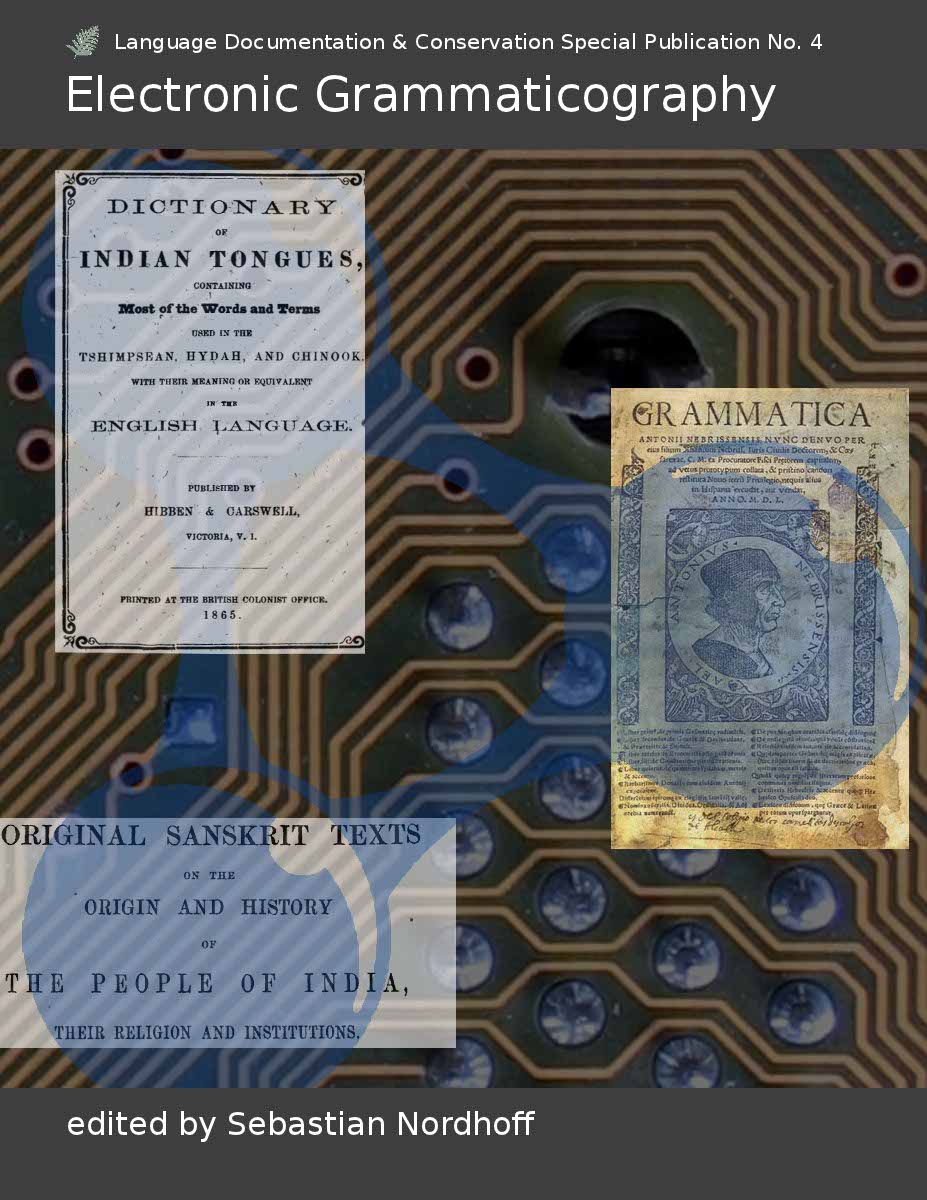
\includegraphics[width=\paperwidth,height=\paperheight,
 keepaspectratio]{hawaiititle.jpg}%
\vfill
}}}


\ohead{\rm\fontsize{9bp}{19.8bp}\selectfont\thepage} % bei den Fontsizes nimmt man erst den Font, die zweite Zahl ist der Font x 1.2
\ihead[
  \parbox{1.5cm}{
  \rm\fontsize{59bp}{70.8bp}\selectfont\thechapter\small
  }
  \parbox{11cm}{
  \begin{flushright}  
	{\thischapteruuheader}
  \end{flushright}
  }
]{\fontsize{9bp}{10.8bp}\selectfont\chapname}

\ihead[\rm\fontsize{59bp}{70.8bp}\selectfont\thechapter]{\fontsize{9bp}{10.8bp}\selectfont\chapname}
\ofoot{\fontsize{9bp}{10.8bp}\selectfont \textsc{Electronic Grammaticography}}
\ifoot[\rm\fontsize{6bp}{7.2bp}\selectfont Licensed under Creative Commons  Attribution License]{Electronic Grammaticography}


\newcommand{\shortauthor}{noauthor}
\newcommand{\longauthor}{noauthor}
\newcommand{\longchapname}{nochapname}
\newcommand{\mytoc}{\stepcounter{chapter}%
% 		    \renewcommand{\chapname}{\longchapname}%
		    \addcontentsline{toc}{chapter}{\longchapname \\ %
						  {\it \shortauthor}%
		    }%
		   }




\pagestyle{scrheadings}
\clearscrheadings % löscht erstmal alles
\clearscrheadfoot
\clearscrplain
\begin{document}  
\AddToShipoutPicture*{\BackgroundPic} 
~
\newpage
\clearscrheadings

\frontmatter\ohead{\rm\fontsize{9bp}{19.8bp}\selectfont\thepage} % bei den Fontsizes nimmt man erst den Font, die zweite Zahl ist der Font x 1.2

\renewcommand{\thischapteruuheader}{\uhheader{xx-xx}{4551}}
 
% \ihead[
%   \parbox{1.5cm}{
%   \rm\fontsize{59bp}{70.8bp}\selectfont{~}\small
%   }
%   \parbox{11cm}{
%   \begin{flushright}  
% 	{\thischapteruuheader}
%   \end{flushright}	
%   }]{}
\chapter*{~}
\noindent

\begin{flushleft} 
{\small
Published as a Special Publication of Language Documentation \& Conservation\\
Department of Linguistics, UHM\\
Moore Hall 569\\
1890 East-West Road\\
Honolulu, Hawai'i 96822\\
USA\\
http://nflrc.hawaii.edu/ldc\\
University of Hawai‘i Press\\
2840 Kolowalu Street\\
Honolulu, Hawai‘i\\
96822-1888\\
USA\\
{\textcopyright} All texts and images are copyright to the respective authors. 2012\\
All chapters are licensed under Creative Commons Licenses\\
Cover design by Sebastian Nordhoff\\
Cover photograph {\em labyrinthine circuit board lines} by Karl-Ludwig G. Poggemann (http://www.flickr.com/photos/hinkelstone/2435823037/) licensed as  CC-BY 2.0 (http://creativecommons.org/licenses/by/2.0/deed.en)\\
Library of Congress Cataloging in Publication data\\
ISBN: 978-0-9856211-1-7\\
http://hdl.handle.net/10125/4547\\
} 
\end{flushleft}
\newpage 
% \renewcommand{\thischapteruuheader}{\uhheader{xx-xx}{4548}}
\renewcommand{\thischapteruuheader}{}
\tableofcontents 
% % \input{intro/intro.tex}
% % \input{intro/intro.bbl}

% \renewcommand{\thischapteruuheader}{\uhheader{xx-xx}{4549}}
\renewcommand\chapname{Contributors}	
\renewcommand\longchapname{Contributors}
\renewcommand\shortauthor{}
\renewcommand\longauthor{}
\chapter*{\longchapname} 
\mytoc{}  

\textbf{Tim Baldwin} completed a BSc(CS/Maths) and BA(Linguistics/Japanese)
at the University of Melbourne in 1995, and an MEng(CS) and PhD(CS) at
the Tokyo Institute of Technology in 1998 and 2001, respectively. He is
currently an Associate Professor and Deputy Head of the Department of
Computing and Information Systems, The University of Melbourne, and a
contributed research staff member of the NICTA Victoria Research
Laboratories. His research interests cover topics including deep linguistic
processing, multiword expressions, text mining of social media, computer-
assisted language learning, information extraction and web mining, with
a particular interest in the interface between computational and theoretical
linguistics.

\textbf{Anne-Marie Baraby} has been working on Innu language for the past thirty years, after having completed her studies in linguistics in the fields of Native American language description and of grammaticography of minority languages. Also working as instructor in linguistics among Innu language teachers, she is presently a part-time teacher in French grammar in the Département de linguistique at the Université du Québec à Montréal 

\textbf{Emily M. Bender} received her PhD in Linguistics from Stanford
University in 2001 and is presently an Associate Professor in the
Department of Linguistics at the University of Washington.  Her
primary research interests lie in grammar engineering.  She is the PI of
the Grammar Matrix project.

\textbf{Cheryl} and \textbf{ H. Andrew Black} are linguistic consultants with SIL Mexico (http://www.sil.org/mexico/00i-index.htm). They previously served with SIL in Peru.  They are adjunct faculty with the Summer Institute of Linguistics at the University of North Dakota (http://arts-sciences.und.edu/summer-institute-of-linguistics/). Andrew earned his PhD in Linguistics from the University of California, Santa Cruz in 1993 and Cheryl earned hers in Linguistics from the University of California, Santa Cruz in 1994.

\textbf{Peter Bouda} finished his M.A. in 2007 at the Institute of General Linguistics
and Language Typology at the Ludwig-Maximilian-University in Munich. He
then worked as a software developer for Linguatec GmbH in Munich and 
later as a freelancer in software development for mobile phones. He is now a
researcher within the project "Quantitative Historical Linguistics" at the University of Munich and is 
responsible for the development of the web application and the database 
design. His research focus is the design and usability of software used 
in linguistic research. He develops Python modules and applications that
 allow linguists to annotate and analyze their data


\textbf{Rebecca Dridan} received her PhD in Computational Linguistics from
Saarland University, Germany in 2009. She is currently employed as a
Postdoctoral Fellow in the Language Technology group at the University
of Oslo, where she is part of the WeSearch project. Her primary
research focus is on combining statistical and linguistic information
to extract meaning from text.


\textbf{Sebastian Drude} is the Scientific Coordinator of The Language Archive (TLA) at the Max-Planck-Institute for Psycholinguistics. He is a documentary / anthropological linguist interested in language technology and infrastructure.  Since 1998, he has conducted fieldwork among the Awetí indigenous group in Central Brazil, participating in the DOBES (Documentation of Endangered Languages) research program from 2000 on.  From 2008 on he was a Dilthey fellow at University Frankfurt, before in November 2011 he went to the MPI Nijmegen joining the leading group of TLA, which hosts the central DOBES language archive and develops tools and infrastructure for linguistics and the digital humanities.

\textbf{Sumukh Ghodke} is pursuing his PhD in the Language Technology Group,
University of Melbourne and is being advised by Assoc. Prof. Steven Bird.
His primary research interest is in database systems for managing large
collections of semi-structured data.
 
 

\textbf{Jeff Good} is Assistant Professor of Linguistics at the University at Buffalo. His research areas include examining the impact of new digital technologies on the practice of linguistics, documentation of languages of Northwest Cameroon, comparative Benue-Congo linguistics, and morphosyntactic typology.



\textbf{Johannes Helmbrecht} studied General and Comparative Linguistics, Philosophy,
and Psychology at the University of Bonn and the University of Cologne. He
received his PhD from the University of Bonn in 1994 with a thesis on the
concept of semantic roles. Areas of research later on were the morphosyntax of
East Caucasian languages, in particular Lak, and personal pronouns and person
marking in general and in North American Indian languages. He finished the
``Habilitation'' with a
thesis on the typology of personal pronouns at the University of Erfurt. He
conducted extensive fieldwork in Daghestan (Russia) and on Hocank, a North
American Indian language of the Siouan family in Wisconsin. He was principal
investigator together with Christian Lehmann of the DOBES project on the
documentation of the Hocank language. Since 2006, he  holds a chair in General
and Comparative Linguistics at the University of Regensburg.


\textbf{Mike Maxwell} is a researcher in grammar description and other computational
resources for low density languages, at the Center for Advanced Study of
Language at the University of Maryland. He has also worked on endangered
languages of Ecuador and Colombia, with the Summer Institute of
Linguistics, and on low density languages with the Linguistic Data
Consortium (LDC) of the University of Pennsylvania.


\textbf{Ulrike Mosel} is professor emerita of General Linguistics at the University of Kiel. After gaining her PhD in Semitic languages at the University of Munich (1974), she started researching South Pacific languages and became an expert in collaborative fieldwork. Her books include /Tolai Syntax /(1984), /Samoan Reference Grammar /(1992, with Even Hovdhaugen), /Say it in Samoan /(1997, with Ainslie So'o). Currently she is working on the documentation of the Teop language of Bougainville, Papua New Guinea. Together with Christian Lehmann, Hans-Jürgen Sasse and Jan Wirrer she initiated the DoBeS language documentation programme funded by the Volkswagen Foundation since 2000.
 


\textbf{Simon Musgrave} is a lecturer in the School of Languages, Cultures and
Linguistics at Monash University. He completed his doctorate at the
University of Melbourne in 2002, and was then a post-doctoral researcher at
Leiden University and an Australian Research Council post-doctoral fellow
at Monash.  His research interests include Austronesian languages, language
documentation and language endangerment, African languages in Australia,
communication in medical interactions, and the use of technology in
linguistic research. Major publications include the edited volumes *Voice
and Grammatical Relations in Austronesian* (2008) and *The Use of Databases
in Cross-linguistic Research *(2009). Simon has also been closely involved
in the Australian National Corpus project from an early stage, serving on
the steering committee for the first stage of the project as well as being
the treasurer of Australian National Corpus Inc.

\textbf{Sebastian Nordhoff}  is a postdoctoral researcher at the Max Planck Institute for Evolutionary Anthropology in Leipzig. He specializes in language contact and language change and the interface of language description and documentation on the one hand and electronic publication on the other. He is a member of the working group on Open Data in Linguistics of the Open Knowledge Foundation, where he works on integrating typological data into the Linguistic Linked Open Data Cloud. 


\textbf{Nicholas Thieberger} wrote a grammar of South Efate, a language from
central Vanuatu and is project manager for the digital archive
PARADISEC. He is interested in developments in e-humanities methods
and their potential to improve research practice and he is now
developing methods for creation of reusable data sets from fieldwork
on previously unrecorded languages. He is an Australian Research
Council QEII Fellow at the University of Melbourne.



% \renewcommand{\thischapteruuheader}{\uhheader{xx-xx}{4550}}
\renewcommand\chapname{Acknowledgments}	
\renewcommand\longchapname{Acknowledgments}
\renewcommand\shortauthor{}
\renewcommand\longauthor{}
\chapter*{\longchapname}   
\mytoc{}
This book is the result of the workshop on Electronic Grammaticography held in conjunction with the 2nd International Conference on Language Description and Conservation at the University of Hawai'i in February 2011. I would like to thank the organizers of the ICLDC conference for accepting this workshop and for taking care of the local organization. I would furthermore like to express my gratitude towards the Max Planck Institute for Evolutionary Linguistics, whose funding and flexibility made it possible for this workshop to be held in conjuction with ICLDC.
\mainmatter

\clearscrheadings % löscht erstmal alles
\clearscrheadfoot
\clearscrplain 
\part{Theory} 

\setcounter{chapter}{0}

\glossSTDmode
\setcounter{exx}{0}\setcounter{footnote}{0}
\renewcommand{\imgpath}{./Good} 

\ohead{\rm\fontsize{9bp}{19.8bp}\selectfont\thepage} % bei den Fontsizes nimmt man erst den Font, die zweite Zahl ist der Font x 1.2
\ihead[
  \parbox{1.5cm}{
  \rm\fontsize{59bp}{70.8bp}\selectfont\thechapter\small
  }
  \parbox{11cm}{
  \begin{flushright}  
	{\thischapteruuheader}
  \end{flushright}
  }
]{\fontsize{9bp}{10.8bp}\selectfont\chapname}
\ifoot[\rm\fontsize{6bp}{7.2bp}\selectfont Licensed under Creative Commons  Attribution License]{Electronic Grammaticography}

\renewcommand{\thischapteruuheader}{\uhheader{2-32}{4528}}
 
\renewcommand\chapname{Deconstructing descriptive grammars}	
\renewcommand\longchapname{Deconstructing descriptive grammars}
\renewcommand\shortauthor{Jeff Good}
\renewcommand\longauthor{Jeff Good

 University of Buffalo}
\chapter*{\longchapname}
\chapterauthor{\longauthor}
\mytoc{}

 


% \parbox{5in}{\small \noindent
% \section{Abstract}
\begin{abstract}
Much work within digital linguistics has focused on the problem of developing
concrete methods and general principles for encoding data structures designed
for non-digital media into digital formats. This work has been successful enough
that the field is now in a position to move past ``retrofitting'' digital
solutions onto analog structures and to consider how new technologies should
actually change linguistic practice. The domain of grammaticography is looked at
from this perspective, and a traditional descriptive grammar is reconceptualized
as a database of linked data, in principle curated from distinct sources. Among
the consequences of such a reconceptualization is the potential loss of two
valued features of traditional descriptive grammars, here termed \emph{coverage}
and \emph{coherence}. The nature of these features is examined in order to
determine how they can be integrated into a linked data model of digital
descriptive grammars, thereby allowing us to benefit from new technology without
losing important features intrinsic to the structure of the traditional version
of the resource.
\end{abstract}
% 
% \bigskip

%%%%%%%%%%%%%%%%%%%%%%%%%%%%%%%%%%%%%%%%%%%%%%%%%%%%%%%%%%%%%%%%%%%%%%%%%%%%%%%%
\section{From recoding to reconceptualizing\label{Intro}}
%%%%%%%%%%%%%%%%%%%%%%%%%%%%%%%%%%%%%%%%%%%%%%%%%%%%%%%%%%%%%%%%%%%%%%%%%%%%%%%%

The field of linguistics is now well aware of the need to use new digital
technologies to encode linguistic data with care in order to ensure its
portability across user communities, computational environments, and even time
\citep{Bir:Sim:03}.\footnote{I
 would like to thank audience members at the Colloquium on Electronic Grammaticography,
 held at the Second International Conference on Language Documentation and Conservation
 at the University of Hawai`i at M\=anoa, February 11--13, 2011, as well an anonymous
 reviewer, for their comments on the work leading to this paper.
 Many of the ideas developed here have been influenced by informal discussions
 with a number of individuals during the last several years,
 in particular Michael Cysouw and Sebastian Nordhoff.}
This has resulted in a
range of work examining the best means through which traditional linguistic
resources can be re-encoded in digital form. Proposals have been made, for
instance, that offer conceptual models and accompanying digital implementations
for lexical resources \citep{BellBird:2000,PoornimaGood:2010}, interlinear
glossed text \citep{BBB:2003,SchroeterThieberger:2006,PalmerErk:2007},
grammatical paradigms \citep{PentonEtAl:2004}, and descriptive grammars
\citep{Good:2004Metadatabase} (see also \citet{Drudetv} and \citet{Thiebergertv}). Other work has gone beyond this to codify general
principles for conducting this kind of research, as seen, for instance, in
\quotecite{Nordhoff:2009} examination of possible ideal requirements for
electronic grammars and in the ``meta-model'' approach to lexical encoding
embodied by Lexical Markup Framework, developed in the context of work on
natural language processing \citep{Francopoulo:2009} (see also
\namecite{WittenburgEtAl:2002} and \namecite{Trippel:2006,Trippel:2009}).

This work has produced important results, and, in particular, has made clear
that, even if important kinds of linguistic data may still await proper study,
the challenges of encoding them linguistically are presumably solvable using
existing technologies, in particular generalized markup systems like XML (see
\namecite[225--227]{Good:CUPHEL} for discussion of XML in the context of
language documentation). Furthermore, it is even possible to extract from this
body of research an informal general procedure for devising new encoding
schemes: (i)~survey existing practice for presenting data in a given domain,
(ii)~devise a conceptual model of the data that can be understood as providing
an underlying form for the surveyed presentation (or ``surface'') forms,
(iii)~relate the various components of that model to linguistic practice,
focusing, in particular, on how they can be derived from more general principles
regarding what constitutes appropriate  methodology for linguistic analysis, and
(iv)~propose a concrete way of encoding that model using archival markup formats
that is as consistent with those general methodological principles as possible.
While I am not aware of any one publication that incorporates the totality of
these procedures, the combination of \namecite{Good:2004Metadatabase} and
\namecite{Nordhoff:2009} can be understood as an illustration of this approach
in the domain of descriptive grammars (see also \citet{Nordhofftv}).

At the same time, the sensible reliance of such work on \emph{existing} practice
makes it ill-suited for considering the ways in which new technologies should
prompt more fundamental reconceptualizations of the kinds of products that the
field of linguistics should produce as a result of technological changes. This
is illustrated, for instance, by \quotecite{PalmerErk:2007} revision to
\quotecite{BBB:2003} proposals for encoding interlinear glossed text. The
latter is sufficient for dealing with interlinear glossed text's traditional
function of providing a succinct analysis of the lexical and grammatical content
of a given stretch of phrasal data. However, it is not well-suited for an
additional function that is clearly desirable (though non-traditional):
automated (or semi-automated) annotation.

The main goal of this paper is to consider how new models for data
encoding---developed independently from the field of linguistics---might prompt
us to consider revisions to our models for producing traditional grammatical
descriptions. In particular, detailed consideration will be given regarding how
the work required to describe a language's grammar on the basis of documentary
products might be done in a highly distributed fashion by making use of emerging
Web technologies (sections \ref{Context} and \ref{Facets}). However, as we will
see, there is a danger when considering such a possibility: The introduction of
a new conceptualization of a linguistic resource, with clear positive features,
may inadvertently lead to the loss of valued features embedded within
traditional models. This requires the development of means to reintegrate what
has been ``lost'' into the new conceptualization, which can be done by
augmenting received technologies with solutions more specific to linguistics
(sections \ref{Coverage} and \ref{Coherence}). However, the solutions discussed
here only allow us to retain part of what would be lost, underscoring that the
transition from traditional products to digital ones must be led by linguists'
needs rather than the non-linguistic agendas that drive the development of most
new technologies (\sref{Conclusion}).

This paper is primarily conceptual in nature, rather than reporting on the
results of a specific technological implementation. Accordingly, at times, it
will be somewhat speculative, though an attempt will be made, whenever possible,
to ground any speculation in relevant existing technological efforts, often from
within linguistics itself. The intended audience for this paper are so-called
ordinary working linguists, rather than those more directly engaged in applying
emerging technologies to linguistic work. At the same time, I hope that some of
its key ideas will be of interest to both groups. Those familiar with work on
the technologies to be discussed will be aware of the fact that some of the
points made here are relatively well-known outside of linguistics. Therefore, in
some places, the aim of the discussion will not be to outline the significance
of these new technologies generally but, rather, to present them in a way that
makes their utility clearer to a documentary and descriptive linguistic
audience---that is, to linguists who are now, or may in the future, be creating
new grammatical descriptions.



%%%%%%%%%%%%%%%%%%%%%%%%%%%%%%%%%%%%%%%%%%%%%%%%%%%%%%%%%%%%%%%%%%%%%%%%%%%%%%%%
\section{The technological context\label{Context}}
%%%%%%%%%%%%%%%%%%%%%%%%%%%%%%%%%%%%%%%%%%%%%%%%%%%%%%%%%%%%%%%%%%%%%%%%%%%%%%%%

While some data encoding technologies (e.g., XML) have become so ubiquitous in
work on language documentation and description as to require little
introduction, the technological context which inspires the present work---that
of the so-called Semantic Web---has not yet been particularly widely employed
within linguistics. The leading idea behind the development of the Semantic Web
is to extend the document-centered World Wide Web to all kinds of data, adding,
in effect, an explicit layer of meaning to a network architecture that was
originally designed to simply link together pages intended to be interpreted by
humans.{\footnote{The Semantic Web Frequently Asked Questions page
({http://www.w3.org/2001/sw/SW-FAQ}) produced by the World Wide Web Consortium
serves as useful introduction to the Semantic Web. See also
\namecite[2--5]{ChiarcosEtAlIntro:2012} and \namecite[129--131]{Moran:2012}
for additional introductory discussions in a linguistic context.}}

Rather than consisting of a monolithic piece of technology, the Semantic Web is
better understood as resulting from the interactions of a set of
logically-independent technological pieces. Some of these are relatively simple
in and of themselves but, nevertheless, provide crucial elements of the
infrastructure needed to augment the World Wide Web with semantic information.
Moreover, since the Semantic Web is intended to build on the World Wide Web,
many of its core technologies are the same as those of the World Wide Web
itself, as seen, for example, in its use of Unicode for character encoding (see,
e.g., \namecite{Anderson:EMELD:2003} and \namecite[345--351]{Gippert:2006} for
discussion of Unicode in a linguistic context). At the same time, in order to
extend the World Wide Web, there are also technologies that underlie the
Semantic Web that are not part of the World Wide Web. The most prominent of
these within work on language documentation and description is almost certainly
Web Ontology Language (OWL), which has been used to express the linguistic
information encoded in the General Ontology for Linguistic Description (GOLD)
\citep{FarrarLangendoen:2003,FarrarLewis:2007,FarrarLangendoen:2009}.{\footnote{The
latest version of GOLD can be viewed at http://linguistics-ontology.org/.}}
GOLD will be returned to shortly below.

The Semantic Web technologies that will play a significant role in the
discussion here are given in \tref{SWTech}. (The first of these, the URI, is
also a World Wide Web technology and likely to be familiar to many readers.) A
brief summary of the relevant function that each takes on is included in the
table, though this description should not be understood to be exhaustive in a
general Semantic Web context. Both in the table, and elsewhere, the presentation
of the Semantic Web and relevant component technologies is simplified somewhat
for the purposes of exposition.

\begin{table}[ht]
\centering
\begin{tabular}{@{}lll@{}}
\Hline
{\sc acronym}	&	{\sc technology}				&	{\sc function}		\\
\Hline
URI				&	Uniform Resource Identifier		&	Unique identification of entities	\\
RDF				&	Resource Description Framework	&	Description of entities				\\
OWL				&	Web Ontology Language 			&	Encoding of general facts 			\\
\Hline
\end{tabular}
\caption{Some Semantic Web Technologies \label{SWTech}} 
\end{table}

Taken together the three technologies listed in \tref{SWTech} allow for (i)~the
unique reference to anything in the real or mental world (e.g., a language, an
utterance, or a phoneme) in the form of URIs, (ii)~the specification of
``facts'' about those entities (e.g., \emph{English is a language} or \emph{this
sentence makes use of a passive construction}) in the form of RDF expressions,
and (iii) the specification of the overall properties of the conceptual model
that the entities and facts are embedded within (e.g., \emph{sentences have
grammatical properties} or \emph{lexical items are comprised of a combination of
sound, meaning, and grammatical properties}) in the form of OWL statements.
While the ability to specify such information falls short of the rich content of
a traditional descriptive grammar, it should be clear
that even this relatively minimal apparatus could allow for the production of a
significant amount of description of a given language's grammar. In particular,
it would permit many of the ``low-level'' facts that are part of any complete
grammatical description to be encoded in a machine-readable form on the Web.

It would be inappropriate to cover the full technical details of URIs, RDF, or
OWL here. However, it will be useful if something can be said about what these
technologies ``look like'' in concrete terms, especially since none of them is a
prototypical instance of a ``technology''. In Semantic Web applications, URIs
look more or less like the familiar Uniform Resource Locators (URLs) associated
with web pages, taking on a form like \texttt{http://example.org/English}. URLs can, in
fact, be understood as a type of URI that both identifies a given entity (e.g.,
a web page or a file) and also specifies how the entity can be found on the
World Wide Web. While Semantic Web URIs look like URLs, and may even behave like
URLs in resolving to a web page when accessed on a browser, strictly speaking
they need not be URLs. In concrete terms, this would mean that if a URI, which
was not also a URL, were entered into a browser, it would not resolve to any web
page (and produce, for example, an error page).

The idea that a URI may look like URL, but not act like one, is potentially
counterintuitive to those accustomed to working with the World Wide Web rather
than the Semantic Web. However, it is a reasonable consequence of attempting to
build an online repository of information on top of the existing Web rather than
in a completely new environment. In this case, the standard Web mechanism for
uniquely referring to a given web page is simply extended for uniquely referring
to \emph{anything}, whether or not it happens to be associated with a web page.
Of course, alternatives are possible. For instance, the Handle System provides
another mechanism for creating unique identifiers (see
\namecite{BroederEtAl:2006} for discussion of the use of the Handle System in
developing linguistic infrastructure).{\footnote{The Handle System is used by
this journal as a means of persistent identification for published papers. For
example, the handle for \namecite{Newman:2007} is 10125/1724. This handle can be
resolved, using an appropriate online service, to a web page where a copy of the
paper can be found. One way to do this is to simply append the handle to
http://hdl.handle.net/, producing the URL http://hdl.handle.net/10125/1724.}}

An important feature of URIs is that they are not merely unique within some
local system, as might be the case, for instance, for identification numbers of
the sort commonly associated with records in a database. Rather, they are
universally unique in the context of the Web, at least when used as intended.
That is, in Semantic Web terms, anything that needs to be referred to gets a
completely unique identifier. The vast proliferation of identifiers that this
entails may, at first, sound problematic. However, one must bear in mind
that the World Wide Web has grown vastly since its first inception without
breaking down, illustrating the durability of URIs as a mechanism for
providing globally unique references.

Turning now to the second technology listed in \tref{SWTech}, Resource
Description Framework (RDF) is a means for making machine-readable three-part
statements, or \emph{triples}, of the form {\sc {subject~predicate~object}}.
The subject is a URI for some entity, the predicate is a URI for a possible
relationship between a subject and an object, and the object consists of either
of a URI or a limited class other objects, such as a text string. Figure
\ref{RDFExample} gives an example of a representation of two RDF triples. The
first (Triple 1) is intended to relate a subject URI referring to the English
language to an object URI referring to the phoneme \emph{p} via a predicate that
states that that phoneme is found in English (i.e., ``English has the phoneme
\emph{p}''). The second (Triple 2) relates the phoneme \emph{p}, now serving as
a subject of a triple, to its standard transcription, the text string ``p'',
serving as the object of the triple (i.e, ``The phoneme \emph{p} has the
transcription `p''').



\begin{figure}[ht]
\centering
\scalebox{.5}{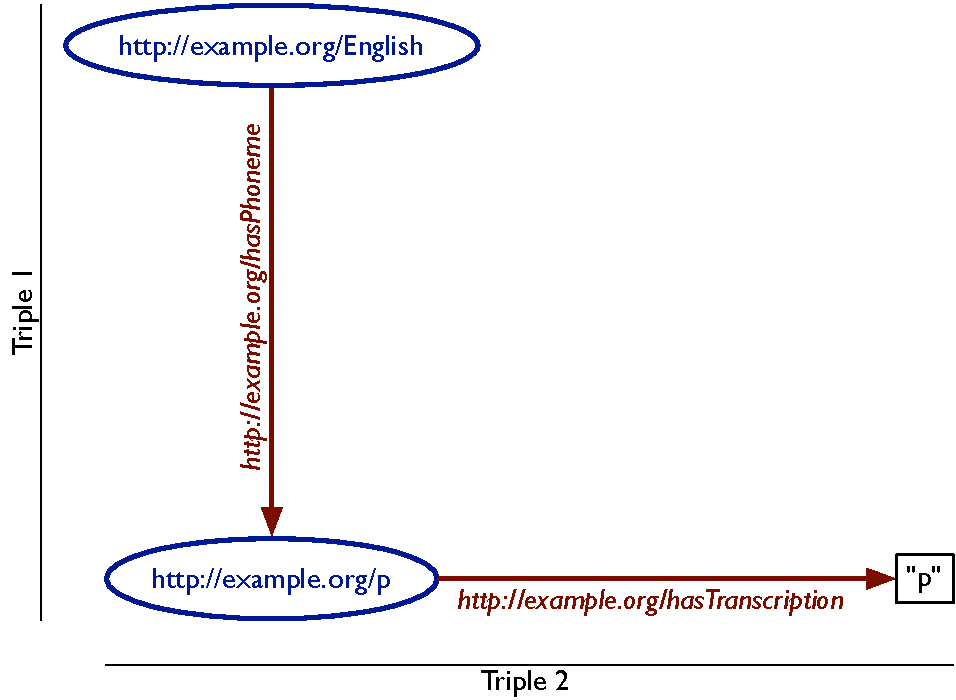
\includegraphics{\imgpath/RDFTriples.pdf}}
\caption{Two RDF triples }
\label{RDFExample}
\end{figure}

RDF has not yet been widely deployed for describing traditional linguistic data,
though there have been some attempts, both as exemplary cases \citep{Simons:2005}
and in working systems \citep{GoodParker:2006} (see also
\namecite[63--65]{Cysouw:2007:Social}).{\footnote{The websites for the World
Atlas of Language Structures (WALS) \citep{WALS:2011}, the World Loanword
Database \citep{WOLD}, and Glottolog/Langdoc \citep{Nordhoff:2012} all allow
data to be exported in RDF format,
though in the case of WALS, this is limited to bibliographical data.}} It has
also seen attention in research in computational linguistics (see, e.g.,
\namecite{IdeEtAl:2003}).

The information encoding model of RDF is, in principle, expressible in a variety
of formats, including a standardized XML format, which facilitates exchange of
data described in RDF. More generally, RDF can be understood as a means for
encoding data that can usefully be modeled in the form of a graph consisting of
nodes connected by labeled arcs, as is seen in \fref{RDFExample}.{\footnote{The
fact that the connections between nodes in RDF representations can be labeled or
``typed'' makes them richer than the connections found in typical hypertext
which merely links documents (or parts of documents) without specifying the
semantic nature of those links. Therefore, while ``hypertext grammars''
\citep[29]{EvansDench:2006} would clearly represent an advance over traditional
grammars, they would fall short of the possibilities afforded by the Semantic
Web.}} Of course, RDF is not the only way of describing data in graph form,
though it is the focus here because of its role as a key means of expressing
``atomic'' statements about entities in the context of the Semantic
Web.{\footnote{Another common way of expressing graphs with labeled arcs in
linguistic work is through the use of feature structures as found, for example,
in Head-driven Phrase Structure Grammar \citep[50--51]{SWB:2003}.}}

An important feature of graphs (whether or not they are expressed in RDF) is
that, as discussed by \namecite{IdeSuderman:2007}, they facilitate the merging
of information from distinct sources. As long as two related sets of data
expressed in graph form use the same identifiers for nodes referring to the same
entities, the two graphs can simply be joined wherever nodes are shared. If we
consider \fref{SWTech}, for instance, one data source could state that English
makes use of the phoneme \emph{p}, while another could associate \emph{p} with a
transcription, with the two being joined by their common node,
http://example.org/p. While this is a relatively trivial example, graph merger
of this kind can become quite powerful when the merged graphs each contain rich
and largely complementary information (see \sref{Disentangling}).

URIs and RDF, when brought together, are key pieces to the idea of creating
significant amounts of \emph{Linked Data}, which is seen as a crucial step
towards the broader vision of the Semantic Web \citep[15]{BizerEtAl:2009}
and provides a useful metaphor for understanding the goals of the Semantic
Web more generally.{\footnote{A workshop on Linked Data in Linguistics was
held on March 7-9, 2012, in Frankfurt, Germany (see http://ldl2012.lod2.eu/)
and resulted in an edited volume \citep{LDL:2012}.}}

The final technology listed in \tref{SWTech} is Web Ontology Language (OWL),
which allows for the expression of \emph{ontologies}. In this context an
ontology can be understood as a means for expressing general knowledge about a
given domain in a form that can be understood by machines. This might include
statements like, \emph{a past tense is a kind of tense} or \emph{a phoneme
inventory is comprised of phonemes}. Basic statements like these could, in fact,
be stated using RDF which is flexible enough to encode both very specific
statements as well as general ones. OWL, however, provides a means for
expressing certain kinds of generalizations that are not standardly expressible
in RDF. In fact, OWL can itself be viewed as an augmentation of RDF in much the
same way as the Semantic Web augments the World Wide Web. To pick one example,
OWL provides a standard way of stating that one property is the ``inverse'' of
another property. This would allow, for instance, a machine to infer that, if
\emph{the phoneme \emph{p} has the transcription `p'}, then \emph{the symbol
`{p}' is a possible transcription of the phoneme \emph{p}}. As discussed above,
there has already been significant work on an OWL-based ontology in the context
of descriptive linguistics in the form of the GOLD project
\citep{FarrarLangendoen:2003,FarrarLewis:2007,FarrarLangendoen:2009}, and there
has also been work using OWL to support the mobilization of descriptive language
materials \citep{BeckEtAl:2007}.

Before moving on, it is important to bear in mind that URIs, RDF, and OWL are
merely specific technical solutions to more general problems. Their significance
in the present context is the way that they are integrated into the larger
vision of the Semantic Web. Of course, the Semantic Web, too, is a specific
technical solution to the broad problem of how information can be shared and
exchanged efficiently. Its relevance for the field of linguistics is twofold.
First, it offers a model for a new way of managing research results in an
increasingly internet-driven data management world. Second, it is a specific
instantiation of such a model with considerable support outside of linguistics,
allowing linguists to take advantage of technological infrastructure that has
already been developed elsewhere.

The next section of this paper will consider how an initiative like the Semantic
Web might prompt us to reconsider what it means to create a descriptive grammar
of a language.




%%%%%%%%%%%%%%%%%%%%%%%%%%%%%%%%%%%%%%%%%%%%%%%%%%%%%%%%%%%%%%%%%%%%%%%%%%%%%%%%
\section{Multiple facets of grammars\label{Facets}}
%%%%%%%%%%%%%%%%%%%%%%%%%%%%%%%%%%%%%%%%%%%%%%%%%%%%%%%%%%%%%%%%%%%%%%%%%%%%%%%%

%%%%%%%%%%%%%%%%%%%%%%%%%%%%%%%%%%%%%%%%%%%%%%%%%%%%%%%%%%%%%
\subsection{Disentangling publication\label{Disentangling}}
%%%%%%%%%%%%%%%%%%%%%%%%%%%%%%%%%%%%%%%%%%%%%%%%%%%%%%%%%%%%%

In this section, I will largely abstract away from the technical details
delineated in \sref{Context} and, instead, focus on how the model embodied by
the conjunction of the technologies in \tref{SWTech} could be exploited to
create new methods for producing grammatical descriptions. In principle, a
number of the ideas developed here could have been put forth decades ago. After
all, many of the key concepts embodied by the Semantic Web (e.g., unique
identification) are hardly new. However, in practice, before the rise of the
World Wide Web, work along such lines would have been largely impossible to
apply concretely to documentary and descriptive research. We have now reached a
point, by contrast, where the development of models that, at one point, would
have been merely speculative or ``futuristic'' can actually be implemented in
specific tools, at least in prototype form. This makes it important for the
field to begin to consider the relevant issues proactively in order to avoid
accidentally adopting technological solutions that might, at first, appear to be
appropriate but which may actually be built on assumptions that will prove
problematic in the long run. (See \namecite[134--138]{BoyntonEtAl:2010} for
relevant discussion in a language documentation context.)

A striking feature of the model that the Semantic Web
offers is the extent to which it leads to a view of scholarly work in
general, and grammaticography more specifically, wherein a number of elements
that were previously intertwined due to the restrictions of paper
publication can now be decoupled from one another. Based on ideas found in
\namecite{Neylon:2010}, we can break down the functions of traditional
``monolithic'' scholarly publications along the lines of what is described
in the following list.


\begin{enumerate}
\label{Publishing}

	\item{{\bf Registering:} Scholarly publishing allows an individual or
	set of individuals to officially establish that they should be associated
	with a given set of ideas or research results. \label{Registering}}
	
	\item{{\bf Filtering:} Scholarly publishing provides mechanisms through
	which a given user can locate the information they are interested in
	both by providing a means through which the quality of a given piece of
	research can be quickly
	assessed and by providing tools for discovery (e.g., through the use of
	keywords).}

	\item{{\bf Curation:} Scholarly publishing works with carefully aggregated
	sets of data that are brought together to tell a specific ``story''.
	\label{Curation}}
	
	\item{{\bf Archiving:} Scholarly publishing produces resources designed to
	be usable in the long-term.}
	
	\item{{\bf Reusing:} Scholarly publishing is associated with standardized
	mechanisms through which research results can be reused in a manner deemed
	acceptable by the research community (e.g., by providing a stable
	citation for a given resource).}

\end{enumerate}
	

Of the five functions of publishing given above, the one of
greatest interest here---and the one which would would seem to be most
profoundly impacted by the technologies discussed in \sref{Context}---is almost
certainly the curatorial function. The traditional model of a
descriptive grammar as a kind of monograph encourages us to see the thousands of
tiny observations that form a complete description as part
of a single research ``outcome''. The graph-based model of the Semantic Web, by
contrast, explicitly makes each of these observations visible as distinctive
connections among discrete objects. This was already schematized in
\fref{RDFExample}, with a relatively simplistic example. Figure \ref{Analysis}
offers something comparable with a more complex example that abstracts away from
some of the more technical aspects of RDF.

\begin{figure}[ht]
\centering
\scalebox{.5}{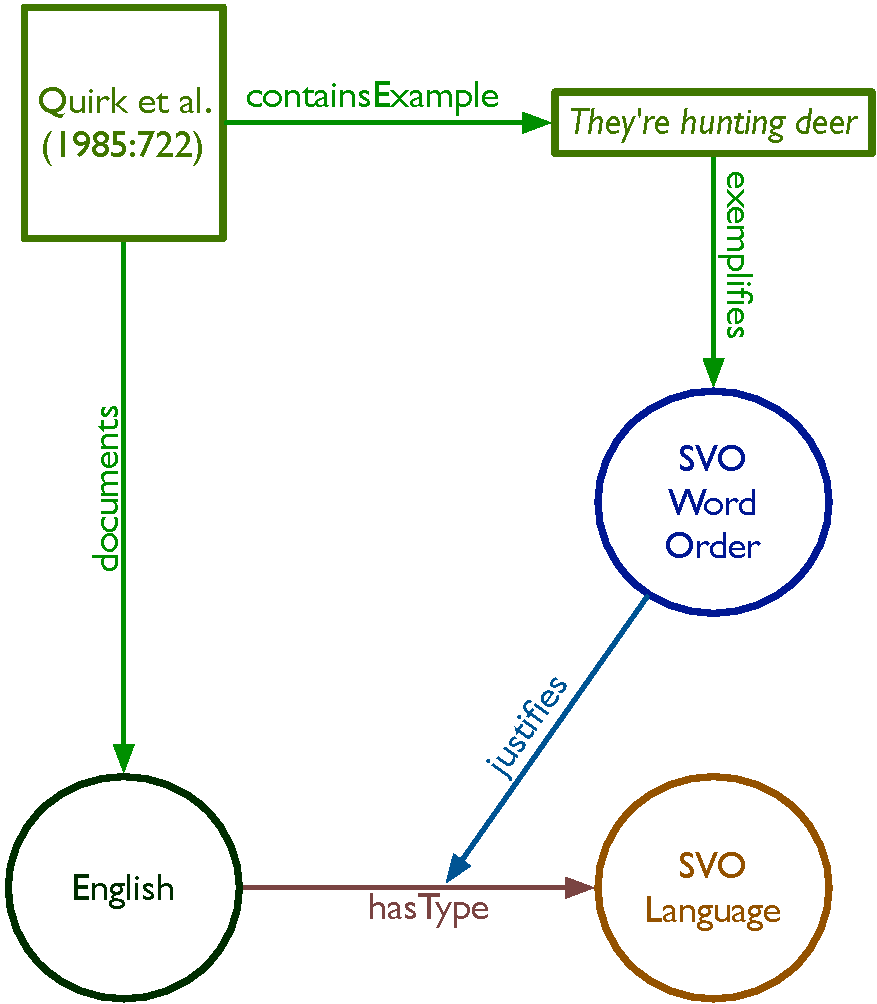
\includegraphics{\imgpath/Analysis.pdf}}
\caption{A fragment of a descriptive grammar in graph form \label{Analysis}}
\end{figure}

\nocite{QuirkEtAl:1985}

Figure \ref{Analysis} represents a set of low-level statements which, when
combined, allow one to make a claim like \emph{English is an SVO language}. At
the top of the figure, an example is indicated as being extracted from a source
that documents the English language. This example is observed to show SVO word
order, which, in turn, justifies the general classification of English as an SVO
language. In RDF terms, this would mean breaking down the classification of
English as SVO into five distinct statements (or triples). There are obvious
elements of simplification involved in the figure, though it should be
sufficient for purposes of exemplification.

By way of further illustration, figure \ref{Genealogy} represents further
information about one of the nodes in \fref{Analysis}, the one representing the
English language. This figure gives reference information for English,
specifically a language code and its genealogical parent. It can be understood
here as representing information about the same entity as described in
\fref{Analysis}, but coming from a different source.

\begin{figure}[ht]
\centering
\scalebox{.5}{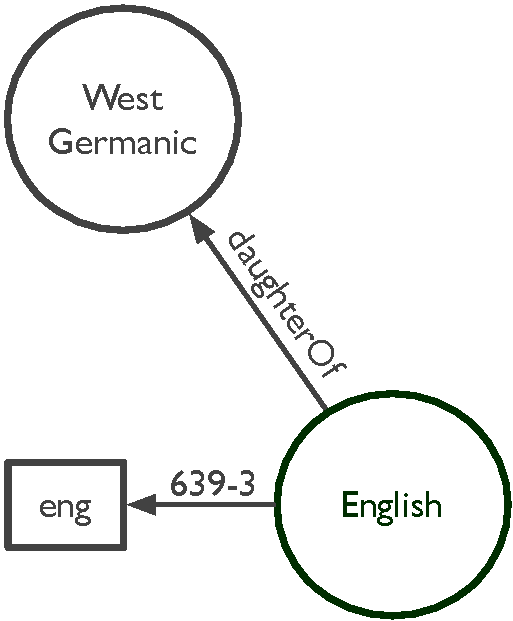
\includegraphics{\imgpath/Genealogy.pdf}}
\caption{Classificatory information for English in graph form \label{Genealogy}}
\end{figure}

Figure \ref{Merger} illustrates one of the positive features of graph-based
representations of information (see also \sref{Context}): The fact that they
allow information from different sources to be straightforwardly merged as
long as common node identifiers are employed. In \fref{Merger}, the content
of figures \ref{Analysis} and \ref{Genealogy} are brought together into a single
graph.

\begin{figure}[ht]
\centering
\scalebox{.42}{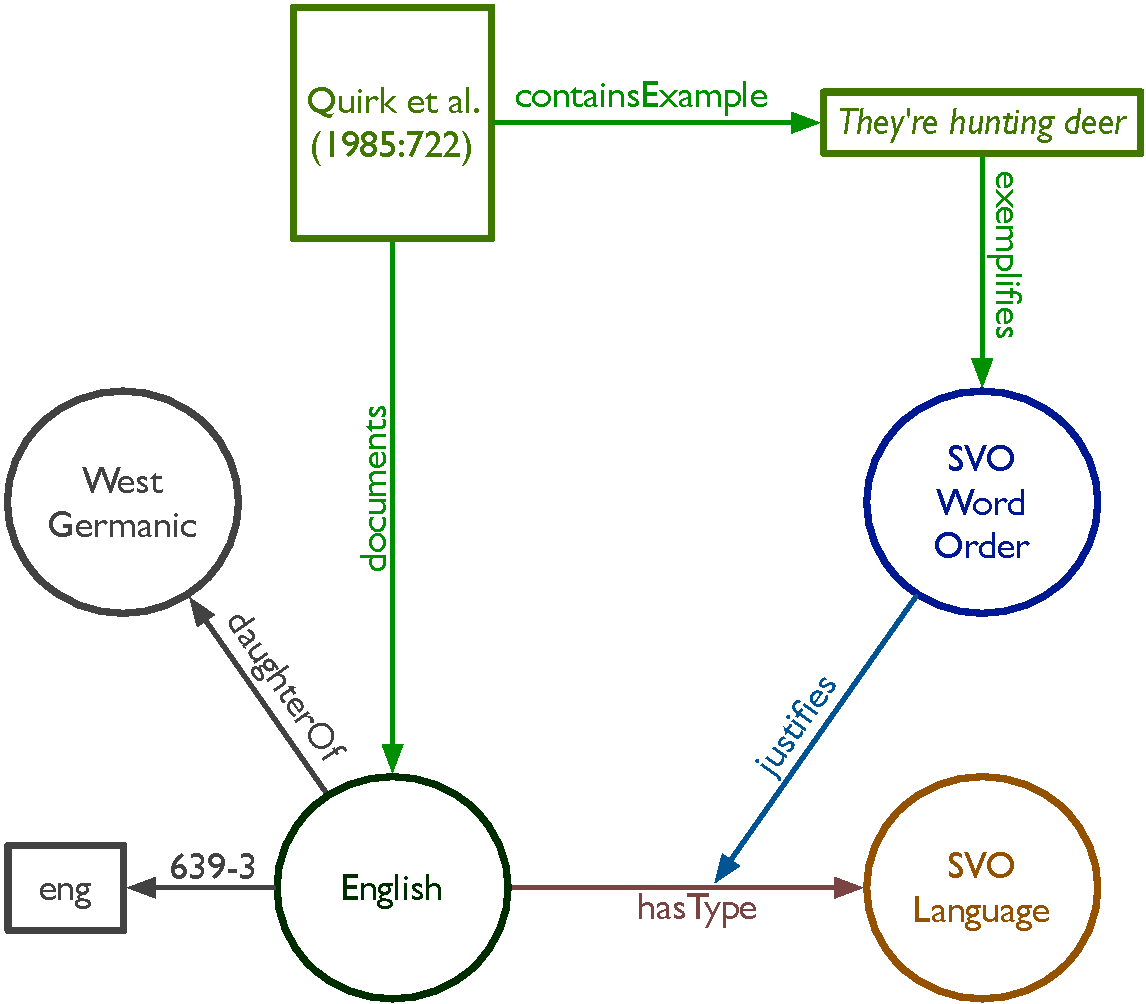
\includegraphics{\imgpath/Merger.pdf}}
\caption{Merging two graphs \label{Merger}}
\end{figure}

Of course, there is nothing particularly innovative about combining related
pieces of information from distinct sources. The power of graph-based
representations like the one seen in \fref{Merger} is the way in which they
allow this process to be, at least partly, automated and the way in which they
make visible the nature of the connections between data sources in a more
precise way than is possible with standard academic citations.

This latter point is of interest here when we consider the inherently
``distributed'' task of writing a descriptive grammar---even if it is only
written by a single author. They are typically the distillation of a number of
years, or even decades, of work on a language and untold numbers of small
observations, preliminary analyses, reanalyses, etc. (see
\namecite[417--418]{Weber:2006} for relevant discussion). Moreover, the
distributed nature of the work involved in grammar writing has become
significantly more pronounced in recent years with the rise of the documentary
paradigm. This has stressed methodological and theoretical separation between
research outputs that can be classified as ``documentary'' from those that are
``descriptive'' (\citeboth{Himmelmann:1998};
\citeboth[168--169]{Woodbury:2011}). The next section will consider then what a
``graph-based'' approach to data might mean for grammar writing, especially in
the context of the newly placed emphasis on documentation. A more concrete way
of looking at this issue would be to ask: How would grammar creation be
different if crafting each of the component statements of a classification like
the one represented in \fref{Analysis} was the responsibility of different
linguists?

Before moving on, it seems worth emphasizing that many of the issues to be
addressed below---for example, ensuring that a grammar has adequate coverage or
that its analyses are coherent---existed long before the development of digital
approaches to research. What has changed is that, now that research can, in
principle, be done in a much more distributed fashion, the utility of general
solutions to problems like these has become more apparent. In the creation of
single-authored grammars, the main control on coherence, for example, has been
the authors themselves. But clearly this concern must be approached differently
if one wants to make use of the time and the skills of ten, or even a hundred,
contributors working on the description of a single language. Moreover, as we
will see in the next section, there has been impetus for grammatical
descriptions to be developed in a more distributed fashion that has arisen
completely independently from the growth of the Semantic Web itself.


%%%%%%%%%%%%%%%%%%%%%%%%%%%%%%%%%%%%%%%%%%%%%%%%%%%%%%%%%%%%%
\subsection{Towards distributed grammar authoring\label{Authoring}}
%%%%%%%%%%%%%%%%%%%%%%%%%%%%%%%%%%%%%%%%%%%%%%%%%%%%%%%%%%%%%

The extent to which the activities comprising documentation and description
should be viewed as easily severable has been questioned (see, e.g,
\namecite[346--348]{Evans:2008}). Nevertheless, it seems uncontroversial that
the possibilities that new technologies offer for creating documentary products
should have a significant impact on the creation of grammatical descriptions
(\citet[24--25]{EvansDench:2006}, see also \citet[120--122]{Good:LDPV}).
Moreover, the documentary paradigm has emphasized the need for a more
collaborative approach to the collection and analysis of language data,
integrating members of speaker communities, as well as experts from allied
disciplines, more directly into the linguist's research activities
(\citeboth[15--16]{Himmelmann:2006}; \citeboth[54--55]{Dwyer:2006};
\citeboth[293--399]{Grenoble:2010}; \citeboth[176--177]{Woodbury:2011}).

While not always emanating from the same fundamental concerns, both of these
ideas share a comparable impact when it comes to research which has as one of
its goals the production of a descriptive grammar. On the one hand, new data
collection and annotation technologies have led to an emphasis on ensuring that
the provenance of a descriptive claim can be straightforwardly verified by
associating it with the relevant supporting documentary materials. Ideally,
these should be in the form of fully transcribed texts as well as audio and
video records (see, e.g., \namecite[571]{Bir:Sim:03};
\namecite[299]{Nordhoff:2009}; \namecite{Thieberger:2009}). This requires tools
and methods for making the ``documentary chain'' from recording to analysis
explicit, which amounts to creating a new set of intermediate linguistic
resources comprising each of the relevant links in that chain. A prominent
example of this is time-aligned annotation, which connects a transcription
directly to the recording containing what is being transcribed. This has
resulted in the widespread use of a relatively new kind of linguistic resource
which encodes documentary and descriptive annotations (see
\namecite{SchultzeBerndt:2006} and \citet{Boudatv}) directly with an indication of start and end
times within a media file that those annotations can be associated with. This is
found, for example, in resources produced by the ELAN annotation tool (see
\namecite{Berez:2007} for a review). What we see in this case is that the task
of annotation, which formerly was disseminated primarily as embedded within
finished products, can now be associated with an ``intermediate'' resource
reflecting an important aspect of the underlying work.{\footnote{Of course,
``intermediate'' objects like this could be created without the aid of new
digital technologies and some of them can be found in archives of field notes.
However, before the rise of the internet, they were not typically made widely
available or as carefully curated.}}

On the other hand, collaborative models for collecting and analyzing linguistic
data cause us to shift perspective from an approach where a single individual is
responsible for all stages of grammatical analysis to one where the various
stages of the documentary and descriptive workflow might be the primary
responsibility of different contributors (see, e.g., \namecite{Thieberger:2004}
and \namecite[461--462]{Bowern:2011} for discussions of workflow). This adds an
additional element of ``decomposition'' to the traditional way of working. In
large part, new data management and communication technologies are a
prerequisite to the practical application of such collaborative models. However,
their ultimate motivation is largely social in nature and emanates from changes
in the conception of what constitutes ethical and appropriate research practices
(see, e.g., \namecite[124--134]{Rice:2006} and
\namecite[201--206]{DobrinBerson:2011}). They can also be understood as a
response to language endangerment, insofar as the impending loss of a language
is understood as a loss not only to linguistics, but to speaker communities and
other disciplines as well. This has, thereby, caused linguists to seriously
consider the need for approaches incorporating a diverse array of stakeholders
in the collection and analysis of language data. Here, then, we see how a set of
changes in practice, driven by social considerations, can at least be partly
supported by new technologies---in this case, technologies which facilitate work
being done in distributed fashion.

Taken together, these two trends place increasing emphasis on the individual
``pieces'' of work involved in the creation of descriptive grammars, as opposed
to treating them as a monolithic whole---the view encouraged by the traditional
publication model. Moreover, independent of developments within work on language
documentation itself, a more distributed approach to work forming the basis of
descriptive grammars, in principle, has an additional potential advantage: It
can facilitate more efficient use of research resources. An individual who is
skilled at transcription may not be adept at morphological analysis, and a
specialist in semantics may not be the ideal person to work on a language's
phonemic system---and this is not to mention the problems that may arise when a
linguist is asked to be not merely a grammarian but also an archivist,
ethnographer, a lexicographer, or even a ``linguistic social worker''
(\citet[14--17]{Newman:1998}, see also \citet[342--343]{Evans:2008}).

We arrive then, at a potential future where we move away from the
publication-centered view of a descriptive grammar as a single-authored
monograph to one where it consists of the compilation of set of ``facts'' about
a language, each associated with a distinct provenance. This view of a
``grammar'' not only has clear connections to the current documentary paradigm,
but it is also consonant with the reconceptualization of data embodied by the
Semantic Web: Research results are ``atomized'' as it were, the barriers to
registering a result (in the sense of developed in \sref{Disentangling}) are significantly
reduced, and the connections between discrete results can be made more explicit.
Of course, it is a long road from the representation of a relatively simple
observation like that seen in \fref{Analysis} to the construction of a graph
representing a ``complete'' descriptive grammar. Nevertheless, we now have a
core conceptual model of such a structure, technology that can implement that
model, and even a field-internal motivation to use such a model. This
means the creation of such an object is no longer simply something only
to be imagined.

Within this broad vision, making the results of research public no longer needs
to be delayed until it reaches the threshold of a ``publishable unit'' (see
\namecite{Broad:1981}) but can be done as soon as a useful observation is made,
even if it constitutes something as simple as the discovery of a new minimal
pair or a single unusual pattern of agreement. Of course, such
``micro-discoveries'' would not be associated with the same level of prestige as
a curated publication.{\footnote{The idea of publishing a ``micro-discovery''
can be clearly connected to the notion of micro-blogging, most prominently
associated at present with the online service Twitter (http://twitter.com),
which has been the subject of work considering how the content of micro-blogs
can be made available not just on the World Wide Web but within the Semantic Web
as well \citep{PassantEtAl:2010}. See also \namecite[64]{Cysouw:2007:Social} for
relevant discussion on the notion of a ``micro-publication'' within work on
language typology.}} What is important is that the Semantic Web, in principle,
can allow them to be associated with the elements of publishing appropriate to
them, e.g., registration, archiving, and reuse (see \sref{Disentangling}), even if
they fall short of the whole traditional publication ``package''.

There are clear potential advantages to reconceptualizing descriptive grammars
as distributed, multi-authored resources. However, it is immediately apparent
that valued features of the traditional descriptive grammar would be lost under
such an approach unless additional measures are taken. In particular, the
curatorial aspect of publishing (see \sref{Disentangling}) imposes various important
characteristics on the assembled ``facts'' which constitute descriptive
grammars, two of which I will focus on here, \emph{coverage} (\sref{Coverage})
and \emph{coherence} (\sref{Coherence}). Of course, these are only parts of what
constitutes a ``good'' grammar (see, e.g.,
\namecite{Noonan:2006,Rice:2006:Grammars}), an issue which will be briefly
returned to in \sref{Deconstructing}.




%%%%%%%%%%%%%%%%%%%%%%%%%%%%%%%%%%%%%%%%%%%%%%%%%%%%%%%%%%%%%
\section{Coverage \label{Coverage}}
%%%%%%%%%%%%%%%%%%%%%%%%%%%%%%%%%%%%%%%%%%%%%%%%%%%%%%%%%%%%%

%%%%%%%%%%%%%%%%%%%%%%%%%%%%%%%%%%%%%%%%%%%%%%%%%%%%%%%%%%%%%
\subsection{Coextensivity and completeness\label{TwoCoverages}}
%%%%%%%%%%%%%%%%%%%%%%%%%%%%%%%%%%%%%%%%%%%%%%%%%%%%%%%%%%%%%

An important aspect of good descriptive grammars is the extent to which their
discussion (i) adequately addresses phenomena represented in the available
documentation on a language and (ii) presents a reasonable overview of a
language's entire grammatical system.{\footnote{By \emph{available
documentation}, I refer to the extent of the documentary resources (e.g.,
recordings, transcribed texts, lexical material, etc.) that those working on the
description of a given language have access to when doing their work.}} I refer
to these properties under the umbrella term \emph{coverage} here, using the term
\emph{coextensivity} for the relationship between a description and available
documentation and \emph{completeness}, to refer to the extent to which a given
description addresses those issues that are taken, at the time of publication,
to be sufficiently central to basic linguistic theory (see
\namecite{Dryer:2006}) that they would be deemed necessary in a ``complete''
description of a language.

Completeness has seen more explicit attention than coextensivity, perhaps most
famously in the form of \quotecite{ComrieSmith:1977} descriptive questionnaire.
This can not only be used as a set of guidelines for ensuring that a grammar has
covered a wide range of grammatical topics deemed descriptively significant
\citep[360]{Noonan:2006} but has even formed the basis of full grammatical
descriptions (such as \namecite{HuttarHuttar:1994}). An important aspect of
completeness is that determining just what constitutes something like a
``complete'' description is within the purview of the general community of
linguists rather than those working on a particular language.

The notion of coextensivity is instead connected to the actual documentation
available in the production of a descriptive grammar (see also \citet{Moseltv}). Therefore, a grammatical
description of a language for which relatively little documentation exists may
be considered to have satisfactory coextensivity even if its level of
completeness is unambiguously inadequate. This would be the case, for instance,
if the only material on a language that was available was a vocabulary list
which might allow for the production of a phonological sketch, but little else.
As such, it is important to distinguish between what is referred as
coextensivity here and what one might call \emph{documentary coverage}. This
latter notion might be used to characterize the extent to which a documentary
corpus actually includes the information needed to create a complete grammar of
a language (see \namecite{Berge:2010} for some discussion), regardless as to
whether or not a descriptive grammar has actually been created on the basis of
that record. A key distinction between coextensivity and completeness is that
what constitutes completeness in a grammatical description can be laid out in
general terms. Adequate coextensivity, by contrast, is dependent upon the
particularities of the available documentation.

Coextensivity has seen not seem as much attention as completeness presumably
because, before the development of the current documentary paradigm, it was
difficult to evaluate due to the inaccessibility of the documentary materials on
which descriptions were based. Even if a given descriptive grammar made clear,
for instance, what percentage of available recordings or texts had been used in
creating it, an inability to examine those texts would have made it essentially
impossible for a reader to gauge the adequacy of its coextensivity. However, to
the extent that the documentary bases of descriptions are expected to become
more widely disseminated, explicit attention to adequacy in coextensivity would
seem warranted. As pointed out by \namecite[25]{EvansDench:2006}, new
technologies are unlikely to result in significantly more analyzed materials
than was previously possible. After all, the time it takes the linguist to
conduct careful analysis will not change in proportion to the amount of material
that can be made available. This means that it is likely to be the case, at
least for the foreseeable future, that grammars will only be based on a sample
of collected materials. Therefore, the extent to which the studied sample may be
representative of the language as a whole will be a significant concern.

An immediate problem with adopting a distributed approach to the production of
electronic grammars is that the model in and of itself does not allow us to
gauge the extent to which a given set of statements about a language's grammar
is adequate with respect to coextensivity and completeness. Properly addressing
such dimensions of coverage has normally been the responsibility of the single
author of a traditional descriptive grammar. Dealing with them in a distributed
context requires us to consider how we can augment Semantic Web (or similar)
technologies with data processing and analysis methods more specific to the
domain of language data. This is the topic of the next two sections, which, in
turn, discuss possible digital approaches to completeness
(\sref{ModelingExternal}) and coextensivity (\sref{ModelingInternal}).





%%%%%%%%%%%%%%%%%%%%%%%%%%%%%%%%%%%%%%%%%%%%%%%%%%%%%%%%%%%%%
\subsection{Modeling completeness\label{ModelingExternal}}
%%%%%%%%%%%%%%%%%%%%%%%%%%%%%%%%%%%%%%%%%%%%%%%%%%%%%%%%%%%%%

In understanding how to ensure adequate completeness in a descriptive grammar,
it is first important to keep clear the fact that just what constitutes a
``good'' description in terms of completeness is not a technological problem but
a scientific one, and it is driven by what is taken to constitute basic
linguistic theory \citep{Dryer:2006} at a given point in time. The key issue here
is not, therefore, deciding what phenomena need to be included in a ``complete''
description, but, rather, how to digitally represent completeness in a way that
facilitates creating grammars with a high degree of completeness and also allows
us to automatically (or semi-automatically) evaluate the level of completeness
attained by some digital descriptive grammar.

Of the problems to be discussed here, dealing with completeness is probably the
easiest since there are already reasonable models to work from, in particular in
work interested in typologically-oriented language comparison.
\namecite{Zaefferer:2006}, for example, describes a system for creating a
cross-linguistic reference grammar database which attempts to balance the need
to ensure that each language is adequately described in its own terms against
allowing comparable features across languages to be compared. In Semantic Web
terms, this approach could be generalized first by formulating a pre-determined
list of elements for cross-linguistic comparison expressed in the form of an
accessible digital object. Then, the completeness of a digital descriptive
grammar could be (at least partly) gauged by the extent to which each member of
that list of elements is or is not associated with a specific RDF statement
relating them to the other observations comprising a digital descriptive
grammar.

Some work has suggested that the relevant elements of comparison should
preferentially be drawn from the onomasiological domain rather than the
semasiological one (\citeboth[122]{Zaefferer:2006},
\citeboth[140--142]{Cristofaro:2006}). However, it seems likely that a full
consensus specification of completeness will need to include specification of of
both functional and formal features. \namecite[28]{ComrieSmith:1977}, for
example, contains a question regarding, in general terms, what kinds of
morphological elements are used to encode the syntactic or semantic functions of
nouns, regardless of the specific functions of those elements. Similarly
categories like \emph{head-marking} and \emph{dependent-marking}, though having
a functional component, primarily target formal variation, but have nevertheless
been the subject of significant typological investigation (see, e.g.,
\namecite{Nichols:1992}).

In any event, while an up-to-date specification of ideal completeness is
lacking, this does not appear to be the result of particular technological
impediments but, rather, a lack of social effort. If there were sufficient
interest, an initial proposal could probably be developed with relatively little
work by examining and selectively merging the topics of a work like
\namecite{ComrieSmith:1977} with more up-to-date surveys of specific typological
phenomena, where available. In particular, the collected grammatical domains
found in \namecite{WALS:2011} would serve as a good recent ``snapshot'' of the
typological state-of-the-art already available in electronic form (see also
\namecite[262--266]{LevinEtAl:2007}).{\footnote{There is at least one instance
of a widely disseminated language description tool, Fieldworks Language
Explorer, which incorporates a kind of grammar model in its design that can
facilitate achieving completeness (see
\namecite{ButlerVolkinburg:2007,Rogers:2010} for reviews). See also \citet{Blacktv}.}}

The specific digital form of an object expressing the components of 
completeness could straightforwardly be based on the familiar notion of a
questionnaire, where each question would be associated with a unique identifier.
These questions would be ``answered'' via an RDF triple linking the topic of the
question to supporting descriptive materials, where relevant via an intermediary
node that would specify a categorial response to the issue raised by the
question. The resulting series of ``links'' between questions and answers could
then function very much like an index in a traditional descriptive grammar,
though with the additional expressive power and utility afforded by digital
technology (see also \namecite[115]{Zaefferer:2006} and
\namecite[162]{Cristofaro:2006}). Though not dealing with the creation of
full-fledged descriptive grammars, relevant work has been done in the domain of
typological database construction. In particular, models have been proposed
which seek to clearly separate the problem of isolating language-specific data
illustrating the presence or absence of a feature from classifying a language
(or construction) on the basis of that data into one of a fixed number of
``types'' \citep{BickelNichols:2002,Cysouw:2007:Social}.

Figure \ref{MergeIndex} augments \fref{Merger} to schematize the integration
of an element associated with completeness with the analysis of a
particular language. The notion of \emph{Basic clausal word order} is treated
as an element that is part of completeness and is introduced into the overall
descriptive graph of English by being associated with the earlier treatment
of English as an SVO language.

\begin{figure}[ht]
\centering
\scalebox{.4}{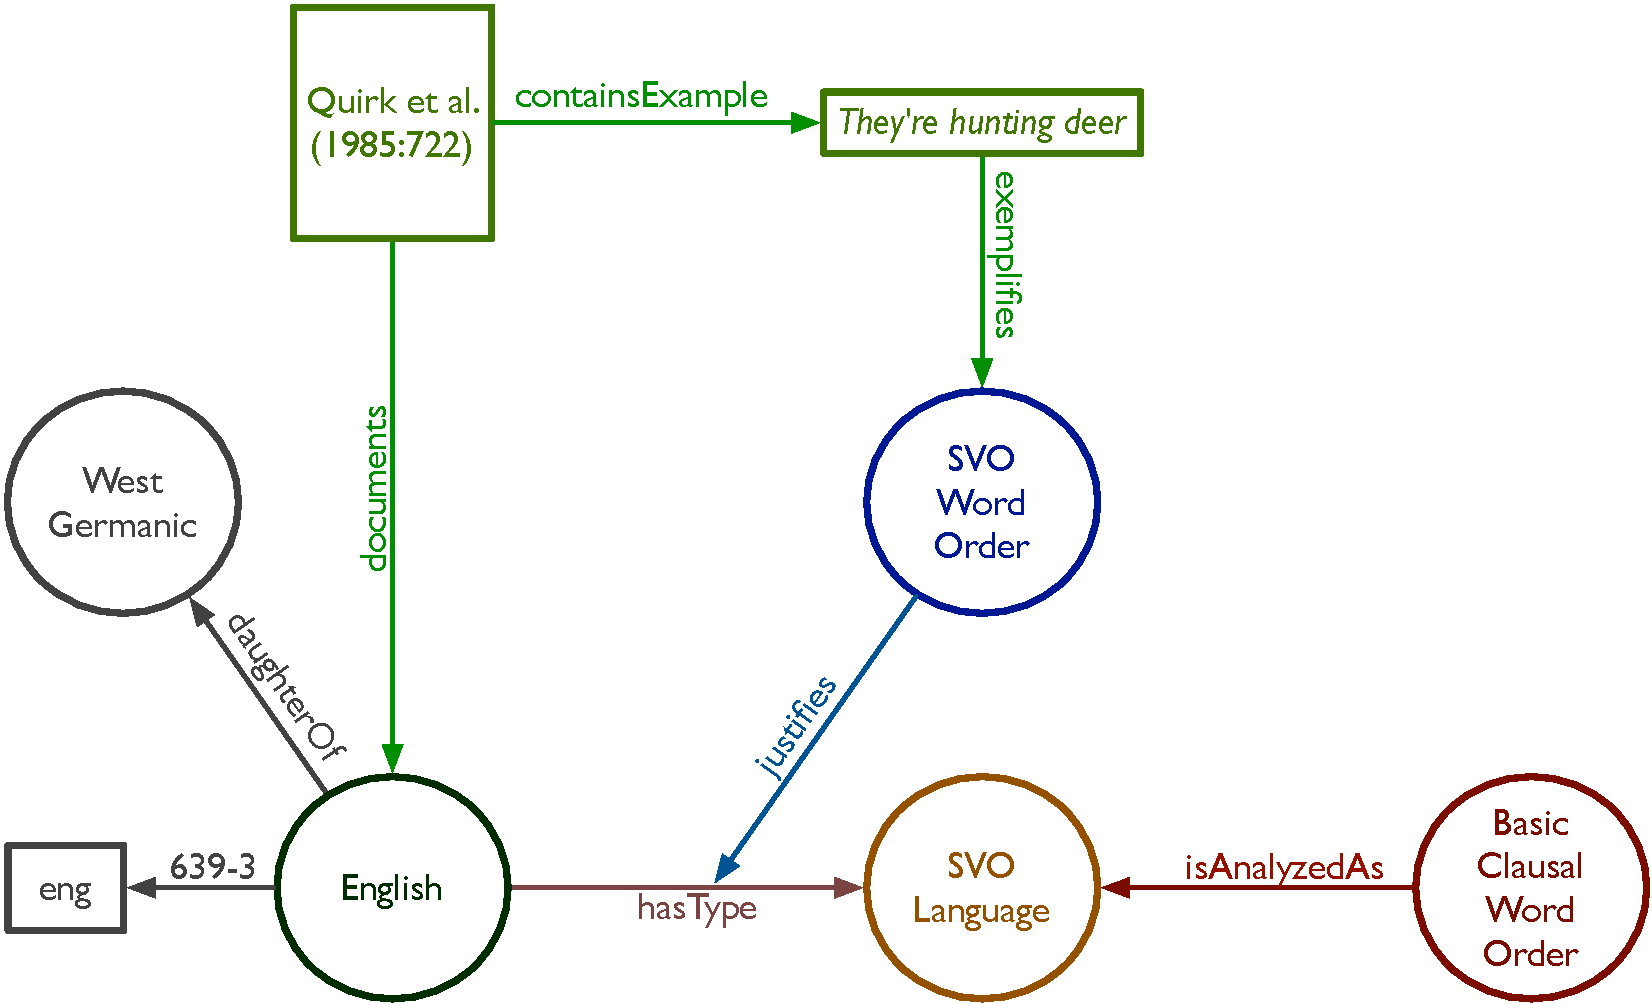
\includegraphics{\imgpath/Indexed.pdf}}
\caption{Adding completeness to a graph-based description \label{MergeIndex}}
\end{figure}

Other elements of completeness could be associated with comparable nodes to what
is seen in \fref{MergeIndex}, though the relationships between the element of
completeness and the descriptive analysis will, of course, not always be as
simple. For instance, if a language showed split word order, this would require
a more elaborate specification in the graph, just as it requires a more
elaborate description in a traditional descriptive grammar. Similarly, if an
element of completeness was associated with a phenomenon not attested in the
language being described, conventions could be adopted to explicitly indicate
its absence, comparable to what is found in the index of
\namecite{Haspelmath:1993Lezgian} (see
\namecite[{\S}2.1]{Good:2004Metadatabase}). Furthermore, just as in a work like
\namecite{ComrieSmith:1977}, where grammatical questions are arranged in a
hierarchy, a full scheme for completeness need not be composed simply of a
``bag'' of questions, but could be specified with additional structure and
information---either using RDF or some other means.

Ultimately, the problem of understanding completeness can be understood as a
kind of data modeling, and better completeness would amount to ``filling out''
more of the elements of an accepted model. For this particular aspect of
descriptive grammars, consensus on the shape of the model itself---whether
digitally encoded or not---appears to be the most difficult issue, with the
technical problems being relatively attenuated.



%%%%%%%%%%%%%%%%%%%%%%%%%%%%%%%%%%%%%%%%%%%%%%%%%%%%%%%%%%%%%
\subsection{Modeling coextensivity\label{ModelingInternal}}
%%%%%%%%%%%%%%%%%%%%%%%%%%%%%%%%%%%%%%%%%%%%%%%%%%%%%%%%%%%%%

Unlike completeness, which must clearly be connected to some community-wide
consensus of what a description should include, coextensivity is
particularized to the documentary record of a language. If the available
documentary information is quite limited, then it might be expected that a
description will be based (more or less) on all of the available data. However,
for languages subject to even a moderate level of investigation, this will often
simply not be possible. Rather, the general goal of the description is not that
it be based on a detailed examination of all of the data. Instead, it
should be based on a sample of the data that results in a description that is
representative of all of the collected data.{\footnote{As will be discussed in
\sref{Coherence}, there are clear connections between coextensivity and
aspects of coherence in descriptive grammars.}}

As mentioned above, there does not appear to have been significant work on how
to measure adequacy of coextensivity. \namecite{Nichols:2005}, however,
considers how much material is needed to produce adequate descriptions
characterized in terms of numbers of words, clauses, and hours, and this would
serve as a good starting point for work on this topic. Ultimately, these
recommendations are probably best considered to be connected to adequacy in
documentation rather than coverage. However, they might serve as proxies for
coextensivity: For instance, her calculation that about 100,000 running
words will allow for ``basic documentation'' suggests that a descriptive grammar
based on a 100,000-word sampling of a much larger corpus is likely to be
sufficient to allow for a reasonable level of analysis of the remaining part of
the corpus by a future investigator, though there will probably still be
significant gaps.

\namecite{Bird:2010} (see also \namecite{Reiman:2010}) describes a documentation
model aimed at under-resourced languages involving the collection of oral texts,
accompanied by oral annotation of a fraction of those texts, and a further
written annotation for a fraction of the orally-annotated texts. While the clear
intention of this process is to provide sufficient annotation (in oral and
written form) of a language to allow the unanalyzed portions to be analyzed in
the future \citep[7]{Bird:2010}, without further research, it seems impossible to
know whether any description creatable on the basis of such a degree of
annotated documentation would actually be sufficient for analyzing the entirety
of the collected materials without the aid of a native speaker. In any event,
the question of what kind of sample of documentary materials can be considered
representative enough to form the basis of a description that would also cover
the remaining materials appears to be an interesting one, and work in this area
would be quite useful for developing general methods for assessing adequacy in
coextensivity.

For transcribed documentary materials, there is at least the possibility of
using a more direct means to assess coextensivity of a description. If a
description can be expressed in a machine-readable form, automated methods could
be employed to apply that description to the entire available dataset (see also
\sref{ConsonanceSec} for related discussion).{\footnote{In principle, these
methods could be applied to untranscribed materials as well if they could
somehow be associated with a reasonable, automatically-derived transcription
using techniques from work on speech recognition. But, of course, that adds a
significant, additional element of complexity.}} The coextensivity of the
machine-readable description could then be considered to be adequate if it can
provide appropriate parses for unanalyzed material. Of course, while some
analytical domains, such as morphological parsing, have seen significant work in
terms of relating traditional documentation to machine-readable parsers (see,
e.g., \namecite{BlackSimons:2008}), most domains of grammar are not yet well
covered. Moreover, while there is at least some relevant work in the domain of
syntax (see \sref{CompatibilitySec}), there seems to be little to no work along
these lines in the domain of phonology (e.g., allowing a user to define a
phoneme inventory and phonotactic constraints and checking to see if
transcriptions are consistent with them).{\footnote{There are, however, tools
that allow one to discover things like phonotactic constraints on the basis of
existing transcriptions, for example Phonology Assistant (see
\namecite{Dingemanse:2008} for a review). Furthermore, the work described
in \namecite{Moran:2012}, though oriented towards typological investigation
rather than description of individual languages, is clearly relevant here.}}

While completeness appears to be representable via data modeling, as discussed
in \sref{ModelingExternal}, this solution does not appear to be applicable to
coextensivity. In particular, the fact that coextensivity is defined in terms of
whatever documentation happens to be available means that it is not amenable to
a treatment involving any kind of general data model. Rather, a more appropriate
approach for modeling coextensivity would appear to be one based on notions from
natural language processing involving the extent to which a parser that has been
``trained'' on a subset of available data can assign correct analyses to data it
has not been trained on (see \namecite{ResnikLin:2010} for overview discussion).\footnote{\namecite{AbneyBird:2010,Bird:2011} offer parallel proposals in
suggesting that one metric for determining whether available documentation is
adequate for capturing the properties of a language is that it is sufficient for
training a machine translation system. } Implementing this kind of approach
generally for digital descriptive grammars is
likely to be quite difficult, however. Creating the relevant kinds of
computational systems, even for well-described languages, is, at this point,
still quite time-consuming and requires resources well-beyond those usually
available to those engaged in language description. Moreover, existing methods are
often heavily reliant on the availability of large quantities of
textual materials, which are simply unavailable for most languages (see also
\namecite{Bird:2011}).




%%%%%%%%%%%%%%%%%%%%%%%%%%%%%%%%%%%%%%%%%%%%%%%%%%%%%%%%%%%%%
\section{Coherence\label{Coherence}}
%%%%%%%%%%%%%%%%%%%%%%%%%%%%%%%%%%%%%%%%%%%%%%%%%%%%%%%%%%%%%

%%%%%%%%%%%%%%%%%%%%%%%%%%%%%%%%%%%%%%%%%%%%%%%%%%%%%%%%%%%%%
\subsection{The components of coherence\label{CoherenceComponents}}
%%%%%%%%%%%%%%%%%%%%%%%%%%%%%%%%%%%%%%%%%%%%%%%%%%%%%%%%%%%%%

A second clear problem with the possibility of taking a distributed approach to
the development of descriptive grammars is that, without specific attention,
they run the risk of becoming incoherent due to distinct conventions and
analyses adopted by different researchers working on pieces of the documentation
or description. Maintaining coherence is, of course, a problem
for all kinds of research, and my goal here will not be to develop the notion
generally, but, rather, to try to specifically model the components of coherence
in descriptive grammars. While the components to be discussed
may not exhaust all of what is required for coherence in
descriptive grammars, those given below appear to represent at least four prominent ones.


\begin{enumerate}%\label{CoherenceList}

	\item{{\bf Consistency in terminology for language-specific categories}: The use
	of terms for language-specific categories is ideally consistently applied
	throughout.}

	\item{{\bf Clarity in terminology for the general audience:} The
	relationships between language-specific categories and comparative concepts
	\citep[in the sense of][]{Haspelmath:Comparative} are ideally made explicit. \label{ClarityP}}
	
	\item{{\bf Consonance of analyses with documentation:} The descriptive
	analyses should ideally be in agreement with what is found in the
	entire documentary record. \label{Consonance}}

	\item{{\bf Compatibility of analyses with each other:} The analyses of
	specific grammatical patterns are ideally compatible with each other
	throughout the description. \label{Compatibility}}

\end{enumerate}

As indicated, the components above represent ideals, and even
single-authored grammars will fail to adhere to them fully. Nevertheless, they
suggest points to pay special attention to if grammatical analysis is to be
distributed since coherence is likely to be an especially problematic area in
this regard.

There are clear connections between certain aspects of coverage and certain
aspects of coherence, at least when these two concepts are understood
informally. This is most clearly seen in relation to coextensivity (see
\sref{TwoCoverages}) and the components of coherence termed \emph{consonance}
and \emph{compatibility} above. Whether or not the coextensivity of a
description would be considered adequate clearly hinges on the extent to which
it is consonant with the documentation and the extent to which all of its
analyses can be brought together into a non-contradictory whole. At the same
time, it seems reasonable to separate these notions. Coextensivity is
intended to reflect the link between available documentation and what
level of description is possible given that documentation, while the
components of coherence are more general than this.
Nevertheless, practically speaking, an important consequence of
the connection between coextensivity and those two components of coherence is
that they may require overlapping technological support.

In the next section, I will discuss how the components of coherence mentioned above could be modeled digitally and discuss existing
technologies that would be relevant for the implementation of those models,
thereby complementing the discussion in \sref{Coverage} and suggesting
additional ways in which the Semantic Web vision might be augmented to
facilitate the creation of digital descriptive grammars in a distributed
fashion. Many of the points to be discussed below should resonate even for those
working on traditional grammatical monographs, but, again, the idea that the
work might be done by many individuals, rather than just one, brings the
relevant issues to the fore. Under such an approach, it will no longer be
obvious who is in charge of the ``quality control'' needed to achieve
coherence, which necessarily prompts us to consider how we might develop means
of ensuring that it is maintained that do not depend on the presence of a
central ``author''.



%%%%%%%%%%%%%%%%%%%%%%%%%%%%%%%%%%%%%%%%%%%%%%%%%%%%%%%%%%%%%
\subsection{Modeling coherence\label{ModelingCoherence}}
%%%%%%%%%%%%%%%%%%%%%%%%%%%%%%%%%%%%%%%%%%%%%%%%%%%%%%%%%%%%%

%%%%%%%%%%%%%%%%%%%%%%%%%%%%%%%%%%%
\subsubsection{Consistency\label{ConsistencySec}}
%%%%%%%%%%%%%%%%%%%%%%%%%%%%%%%%%%%

In discussing \emph{consistency} for the terminology used in a grammatical
description, I refer only to consistency for the terms used to describe the
categories found in the language in question. This dimension of coherence,
therefore, is not intended to apply to the use of terms for general linguistic
concepts, of the sort contained within the GOLD ontology, which I treat as
relevant, instead, to the notion of \emph{clarity}.
The distinction between language-specific categories and general linguistic ones
is not always well-maintained within descriptive grammars, though it is found,
for instance, in \namecite[11]{Haspelmath:1993Lezgian} (on the basis of a
practice employed in \namecite[13]{Comrie:1976}). In that grammar, capitalized
terms are used for language-specific categories and lower-case terms for general
linguistic notions (see \namecite[\S 2.1]{Good:2004Metadatabase}).

Ultimately, the issue of maintaining consistency in a description can, in large
part, be understood as a problem of terminology management (or
\emph{terminography}), which is a distinctive area of research in its own right
(see, e.g., \namecite[1--3]{WrightBudin:1997} and
\namecite[115--159]{Cabre:1999}). Terminology management has some overlap with
lexicography. However, it is primarily oriented with relating concepts to forms,
rather than forms to concepts, as is typical of lexicography
\citep[7--8]{Cabre:1999} (thus making it more comparable to the onomasiological
rather than the semasiological approach to descriptive grammars).

Descriptive linguistics generally already involves a fair amount of informal
terminology management (as evidenced, for instance, by ubiquitous glossing
abbreviation lists and efforts like \namecite{LGR:2008}). Therefore, even if we
did not adopt a distributed approach to the writing of descriptive grammars, the
field could clearly benefit from more robust (and ideally partially automated)
techniques for managing the terms used to describe a given language.
Furthermore, once one considers the possibilities for more distributed
authorship, such techniques would seem to become a necessity in order to
facilitate harmonization of terms across content contributors, whether these are
in Semantic Web form from the start or partial Semantic Web annotation is
attempted for legacy resources. Work of the latter sort could specifically build
on existing research in the area of (semi-)automated term extraction (see
\namecite{AhmadRogers:2001}).

On the whole, technological support for the consistent use of terminology within
a grammatical description appears to be largely underdeveloped. However, it
seems like a potentially profitable area in which to focus efforts in the near
term. This is due to the possibility to make use of existing work on terminology
management in general, as well as on terminological support for the component of
descriptive coherence termed \emph{clarity} here. This latter
area of research will be discussed in the next section, and it can likely serve
as a useful model for the development of tools facilitating consistency in the
use of language-specific terminology, as will be briefly discussed below.



%%%%%%%%%%%%%%%%%%%%%%%%%%%%%%%%%%%
\subsubsection{Clarity\label{Clarity}}
%%%%%%%%%%%%%%%%%%%%%%%%%%%%%%%%%%%

A well-known problem of linguistic description is the use of the same word to
refer to different grammatical concepts or the use of different words to refer
to the same concept across descriptions (see, e.g.,
\namecite[{\S}1]{CysouwEtAl:2005} and \namecite[114]{Zaefferer:2006}). In either
case the potential for confusion is clear, and the issues are especially acute
for work attempting to automate, or partly automate, language comparison on the
basis of digital materials.

This has been one of the key motivations behind the development of the
GOLD ontology
\citep{FarrarLangendoen:2003,FarrarLewis:2007,FarrarLangendoen:2009}, already
discussed in \sref{Context}, which represents the longest-running effort for the
exploitation of Semantic Web technologies for use in descriptive linguistics.
GOLD provides a set of standardized concepts relevant to grammatical description
that can be used to formally define a term used in a language description in
general linguistic terms. For instance, it would allow for the specification
that the English Past Tense verb form expresses a meaning that can be reasonably
related to the general notion of \emph{past tense} specified in GOLD. Of course,
in this case, the terminology is not particularly problematic. However, when
dealing with a form like the Latin Perfect, which would be generally
characterizable as a combination of \emph{perfective} and \emph{past}, rather
than a \emph{perfect} \citep[13]{Comrie:1976}, being able to relate a
language-specific term to more general categories with readily-accessible
definitions, as GOLD allows for, is clearly valuable.

GOLD both provides a standardized termset (with associated URIs for each term)
and structures the members of the termset into an ontology (consisting of a
taxonomy plus some additional information) in order to facilitate automated
processing of linguistic data. Such an ontology is not a strict requirement to
achieve clarity in use of terminology, and a somewhat simpler model is provided
by ISOcat
\citep{KempsSnijdersEtAl:2008:LREC,KempsSnijdersEtAl:2008:ehum}.{\footnote{http://www.isocat.org/}}
ISOcat provides an open registry for data categories relevant
to linguistic resources, allowing an individual linguist or groups of linguists
to publicly register the terms they use and associate them with basic
descriptions of the meaning of the terms. It also provides a unique identifier
for each term which can be used in a Semantic Web context.{\footnote{While
ISOcat's structure does not allow for the specification of an ontology for its
categories, there has been work attempting to develop a degree of ontological
structure around the ISOcat categories in a parallel resource
\citep{WrightEtAl:2010,WindhouwerWright:2012}.}}

ISOcat has a somewhat more ``open'' model than GOLD, insofar as it allows
different groups to register their own categories. By contrast, the addition of
new categories to GOLD is more centrally managed. At the same time, GOLD's
community model explicitly allows for different subcommunities of linguists to
extend the ontology to suit their specific needs (see
\namecite[53--55]{FarrarLewis:2007}). Taken together, an open registration
system like ISOcat in conjunction with tools making it straightforward to
associate an ISOcat category with the appropriate GOLD concepts could provide a
significant degree of support for some of the issues relating to consistency in
the use of terminology discussed above.

There does not yet appear to be significant use of resources like GOLD or ISOcat
to enhance traditional descriptive work. However, due to the efforts that have
been expended on their development, terminological clarity can probably be
considered, at present, the best supported component of coherence discussed
here.




%%%%%%%%%%%%%%%%%%%%%%%%%%%%%%%%%%%
\subsubsection{Consonance\label{ConsonanceSec}}
%%%%%%%%%%%%%%%%%%%%%%%%%%%%%%%%%%%

The development of the documentary paradigm has altered expectations regarding
the extent to which the data on which a description is based should be
accessible. This brings to the fore an issue with respect to coherence which was
always present but was often of little practical significance: To what extent is
a given description, which will often be based on a detailed examination of only
a subset of documentary materials, in agreement with the entire body of
available documentation for a language? Section \ref{ModelingInternal} discussed
related issues from the point of view of ensuring adequate coextensivity.

Because the documentary expectations that have made this problem a practical
concern are relatively new, this issue does not appear to have received
significant attention. The focus, up to the present, has instead been on
developing methods through which a given descriptive claim can be verified on
the basis of supporting documentation in a relatively richly annotated corpus
(see, e.g., \namecite{Thieberger:2009}). But, in the long run, it would also be
ideal if it were possible for sparsely annotated documentation to be
automatically processed on the basis of existing connections between
documentation and description in order to locate possible cases of discord
between the documentation and the description. This processing could involve
such things as, for example, the detection of phonological processes that fail
to apply as expected, the discovery of members of a morphological paradigm which have not been accounted for, or flagging uses of a discourse marker that do not match
its description.

These are, of course, difficult tasks to the extent that they require the
development of sophisticated parsers based on machine-readable grammars---the
descriptive grammatical equivalent of debugging software (see also
\sref{ModelingInternal}). One potentially promising relevant line of work in
this regard involves automated processing techniques that make use of manual
annotation of a fragment of a corpus combined with \emph{active learning} in
which the user provides feedback to an automated system to help improve its
performance. This has been applied to the domain of interlinear glossed text
\citep{BaldridgePalmer:2009,PalmerEtAl:2009,Palmer:2009,PalmerEtAl:2010} and
could, in principle, be applied to other domains as well, reducing the effort
required to create useful parsing tools for a given language. However, the path
from experimenting with these methods to providing robust tools for checking the
complicated relationships involved in consonance between documentary products
(e.g., transcribed texts) and descriptive ones (e.g., a complete grammar based
on those texts) is likely to be a relatively long one. (A different line of
research involving machine-readable grammars, more relevant to the notion of
compatibility, but with potential applications to consonance as well, will be
discussed below.)

An open question in research along these lines is where the most effective
``balancing point'' might be for manual versus automatic annotation and whether
or not even relatively simple types of annotation might facilitate the use of
automated methods in ways that make more effective use of an expert's time. For
instance, it will often be the case that documentary recordings will contain
stretches of different languages, most typically a language of wider
communication and a language being documented. Annotating which stretch is in
which language may be able to be done by someone without special linguistic
expertise on a subset of the recordings to train a machine to do the work across
the whole documentary corpus. This would give an expert linguist a head-start on
more complex kinds of annotation by making it easier for them to locate the most
important stretches of recorded data. The maintenance of consonance in the
relationship between documentary products and derivative descriptive ones would,
thereby, be facilitated. Such a scenario suggests the possibility that taking
full advantage of a more distributed approach to grammatical description may
require us to consider crafting non-prototypical documentary products---in this
case a very sparse kind of linguistic annotation.{\footnote{This scenario also
recalls recent work, such as \namecite{SnowEtAl:2008}, which suggests that
internet marketplaces where workers can be recruited to perform relatively
simple annotation tasks at much lower rates than individuals with linguistic
training may be useful for language research. However, see
\namecite{FortEtAl:2011} for discussion of ethical complications potentially
associated with using such marketplaces, related to the limited rights and wages
typically granted to workers.}}




%%%%%%%%%%%%%%%%%%%%%%%%%%%%%%%%%%%
\subsubsection{Compatibility\label{CompatibilitySec}}
%%%%%%%%%%%%%%%%%%%%%%%%%%%%%%%%%%%

The final dimension of coherence to be discussed here, compatibility, has
already seen some attention in the computational linguistics literature in the
area of grammar engineering, which seeks to create machine-readable versions of
formal grammars (see, e.g., \namecite{Bender:2008}). Among other things, these
grammars allow linguists to automatically test the extent to which their
analysis of a given phenomenon interacts with other analyses as expected,
something which is more or less impossible to do by hand.{\footnote{Grammar
engineering can also play a role in maintaining consonance, insofar as it can help locate instances of data that
cannot be analyzed at all by a given formal grammar, suggesting gaps in a
description.}} Moreover, there have been efforts to ensure that grammar
engineering work done for better-resourced languages can be used to facilitate
the development of machine-readable grammars for lesser-resourced languages
\citep{BenderEtAl:2010}, addressing an issue raised at the end of
\sref{ModelingInternal} in the discussion of coextensivity. Such tools can even
potentially play a role in helping linguists choose among competing descriptive
hypotheses \citep{Bender:2010}.

\namecite{Bender:2008:Wambaya} reports the results of work which made use of a
general grammar engineering system to create a machine-readable grammar for a
language typologically quite distinct from those languages that have informed
most computational research. Strikingly, it was possible to create a reasonable
new machine-readable grammar for this language in a timeframe of about six
weeks. This is, of course, only a small fraction of the time it takes to write a
traditional descriptive grammar. It suggests that work in grammar engineering
has reached a point where relatively limited collaborations between linguists
specializing in this area and those working on underdescribed languages may
yield worthwhile results for language description with respect to ensuring
compatibility among analyses. More generally, this work provides a model for how
to move forward in the development of computational techniques to facilitate the
creation of digital descriptive grammars: Lessons learned from the development
of computational tools for better-resourced languages, often at great cost, can
ultimately be applied to lesser-resourced languages at much lower cost (see also
\citet{Bendertv}).

The work described above is primarily focused on syntactic phenomena. Comparable
tools exist for some aspects of morphophonological analysis (see, e.g.,
\citet{BlackSimons:2008} and \citet{Maxwelltv}), though there has not yet been much work on
integrating tools from each of these domains (though see
\namecite{BenderGood:2008} for some discussion of possibilities). Furthermore,
other domains of grammar do not appear to be well-supported yet at all, with
phonology standing out as an area where the lack of obvious tools does not seem
to present major technical problems but, rather, results from a lack of
dedicated effort (though see \namecite{Moran:2012}). For example, a tool allowing a linguist to specify phonotactic
constraints and ensure their overall compatibility would appear to be much more
straightforward to develop than the already existing tools supporting syntactic
analysis mentioned above. Nevertheless, to the best of my knowledge no such tool
exists. (See also \sref{ModelingInternal}.) In other domains, like semantics and
pragmatics, the tool gap is less surprising given the difficulties of conducting
even informal descriptive work in these areas.

While the discussion here has been primarily in terms of issues regarding
parsing language data, some computational systems are designed to be
bidirectional, both parsing and generating language data (see
\namecite[6]{BenderLangendoen:2010} for discussion relevant in the present
context). While I am not aware of specific proposals in this regard, the ability
of such systems to generate data has potential applications for testing
compatibility (as well as consonance) of grammatical analyses adopting
onomasiological approaches. This would require a machine-readable means to
describe the relevant ``functions'' which would serve as an input for the
generation of predicted forms in a given language. The generated forms could be
compared against attested forms to gauge the extent to which they match each
other.



%%%%%%%%%%%%%%%%%%%%%%%%%%%%%%%%%%%%%%%%%%%%%%%%%%%%%%%%%%%%%%%%%%%%%%%%%%%%%%%%
\section{Conclusion\label{Conclusion}}
%%%%%%%%%%%%%%%%%%%%%%%%%%%%%%%%%%%%%%%%%%%%%%%%%%%%%%%%%%%%%%%%%%%%%%%%%%%%%%%%

%%%%%%%%%%%%%%%%%%%%%%%%%%%%%%%%%%%%%%%%%%%%%%%%%%%%%%%%%%%%%
\subsection{Building on existing infrastructure}
%%%%%%%%%%%%%%%%%%%%%%%%%%%%%%%%%%%%%%%%%%%%%%%%%%%%%%%%%%%%%

Overall, we have seen above that, if we take the distributed model of research
implied by Semantic Web technologies seriously, we are presented with the
problem of losing desirable characteristics of traditional resources not
embedded within the design of the Semantic Web itself. However, with appropriate
conceptual models of key components of a traditional resource, we can devise
explicit characterizations of what we have lost which allow us to see how we can
augment the Semantic Web (or any comparable endeavor) in ways that reincorporate
the ``missing'' features into our new kinds of resources.

In focusing on coverage and coherence, the overall vision that emanates from
this discussion is one where Semantic Web technologies would form a basic
infrastructure to express statements in ways that make them straightforwardly
registrable and reusable, but where the set of statements comprising a
grammatical description would be subject to additional data processing and
validation. This would involve techniques ranging from the development of formal
data models (to help verify completeness), to the deployment of tools for
terminology management (to help ensure consistency), to the use of
machine-readable formal grammars (to help test for compatibility).

At the same time, significant areas have been identified where tool support or
appropriate models of practice are lacking, though a path to developing those
tools or models can be outlined. This was seen, for instance, in the domain of
coextensivity, where there has been relatively little research on determining
what an appropriate documentary ``sample'' might look like. It was also seen in
the domain of consonance where tools for verifying that nowhere in the
documentation is a description contradicted have not received serious attention on
either the conceptual or implementation side. In both cases, methods from
natural language processing were put forth as presenting possible solutions to
these problems.

Nevertheless, a significant result, I believe, of this survey is the extent to
which many existing technologies provide models (if not necessarily
``off-the-shelf'' tools) for how we might go about developing a tool ``ecology''
(see \namecite{Good:ToolEcology}) for distributed grammatical description with
less effort than might appear to be needed at first. Importantly, even if a
given tool type requires re-implementation to be usable in a documentary and
descriptive context, modeling a new tool on an existing one is likely to save
considerable time and resources, when set against developing it completely anew.



%%%%%%%%%%%%%%%%%%%%%%%%%%%%%%%%%%%%%%%%%%%%%%%%%%%%%%%%%%%%%%%%%%%%%%%%%%%%%%%%
\subsection{Deconstructing \emph{our} problems\label{Deconstructing}}
%%%%%%%%%%%%%%%%%%%%%%%%%%%%%%%%%%%%%%%%%%%%%%%%%%%%%%%%%%%%%%%%%%%%%%%%%%%%%%%%

To conclude, this has paper has been intended to be an exercise in what one
might call ``theoretical'' electronic grammaticography (though grounding the
discussion in specific relevant technologies). While its starting point (see
\sref{Context}) was a technical discussion of the Semantic Web, ultimately its
specific technical details were of less importance than the model that it
provided for a more distributed approach to data dissemination and curation,
which has clear potential applications for many areas of scholarship, but
especially descriptive grammars. This is due to their complexity in terms of the
relationship of descriptive claims to documentation, the breadth of their
subject matter, and the interconnectedness of the elements of description.

While the discussion here has been framed as one where the distribution of the
work of describing a language is dispersed across multiple contributors, the
long-term nature of most descriptive work also means that it is distributed
across time, even if there is only a single main creator. Because of this, many
of the models and techniques described here would certainly also be of value in
cases where effort is expended primarily by one person, but over a long enough
period that they may find it difficult to keep track of their own progress.

Two particular issues were the focus here, coverage and coherence. These are
undoubtedly important aspects of traditional descriptive grammars. However, it
should be emphasized that they are far from the whole story. For instance, one
of the criteria listed by \namecite[396]{Rice:2006:Grammars} as an aspect to
writing an effective grammar is ``richness of illustration'', a clearly
important concern not considered here at all.

Moreover, the framework introduced here does not allow for the expression, in
any straightforward way, of the idea that languages have a basic ``plan'' or
structural ``genius'', to borrow from the famous formulation of
\citep[127]{Sapir:1921}. This idea has been reflected in the intuitions of both
formal and descriptive linguists (see, e.g., \namecite[6--9]{Baker:1996} and
\namecite[3--4]{EvansDench:2006}). However, it is difficult to imagine how it
could be expressed in the deliberately reductionist framework of the Semantic
Web, making it clear that we should not understand a reconceptualization process
like the one offered here as a means of replacing our traditional understanding
of what makes a descriptive grammar ``good''. Rather, it should be seen as an
exercise in understanding how we can use technology to enhance what we already
know to be good (see also \namecite[42--43]{DobrinEtAl:2009}).

Ultimately, the goal of a study like this one is not to set our agenda on the
basis of what a given technology offers but, rather, to clarify which existing
technologies can fulfill our needs and to map out plans for the creation of new
technologies. The Semantic Web may have prompted consideration of many of the
ideas discussed here, but it cannot serve as a substitute for crafting a vision
for the future of linguistic resources with our own values serving as its
foundation.



% \psmall
% 
% \hfill Jeff Good
% 
% \hfill jcgood@buffalo.edu

\documentclass{article}
\usepackage[utf8]{inputenc} % please use UTF8 encoding
\usepackage[T1]{fontenc} 
\usepackage{gb4e}

\begin{document} 
% This file was converted to LaTeX by Writer2LaTeX ver. 1.0.2
% see http://writer2latex.sourceforge.net for more info
\documentclass[letterpaper]{article}
\usepackage[ascii]{inputenc}
\usepackage[T3,T1]{fontenc}
\usepackage[english]{babel}
\usepackage[noenc]{tipa}
\usepackage{tipx}
\usepackage{amsmath}
\usepackage{amssymb,amsfonts,textcomp}
\usepackage[top=0.4917in,bottom=0.7874in,left=0.9839in,right=0.9839in,includehead,head=0.4925in,headsep=0.4528in,nofoot]{geometry}
\usepackage{array} 
\usepackage{hhline}
\usepackage{hyperref}
\hypersetup{colorlinks=true, linkcolor=blue, citecolor=blue, filecolor=blue, urlcolor=blue}
\usepackage{graphicx}
\begin{document}
\clearpage\setcounter{page}{1}\pagestyle{Standard}

\end{document}


\end{document}



\glossSTDmode
\setcounter{exx}{0}\setcounter{footnote}{0}
\renewcommand{\imgpath}{./Nordhoff}
\renewcommand{\thischapteruuheader}{\uhheader{33-62}{4529}}

\renewcommand\chapname{Grammars as form-meaning-pairs}	
\renewcommand\longchapname{The grammatical description as a collection of form-meaning-pairs}
\renewcommand\shortauthor{Sebastian Nordhoff}
\renewcommand\longauthor{Sebastian Nordhoff\\ Max Planck Institute for Evolutionary Anthropology}
\chapter*{\longchapname}
\chapterauthor{\longauthor}
\mytoc{} 
 
\begin{abstract}
This paper analyzes the structure of books containing grammatical descriptions and builds up on work by \citet{Good2004}. It argues that the discussion of morphology, syntax, semantics, and intonation found in grammatical descriptions can be seen as a collection of interdependent form-meaning-pairs. These form-meaning-pairs form part of the larger structure of frontmatter, mainmatter and backmatter \citep{Mosel2006craft} and have themselves an internal structure which includes, among other things, linguistic examples as formalized by \citet{BowEtAl2003}.
\end{abstract} 

\section{Introduction}
In this paper I will be concerned with the structure of a certain genre of texts, namely grammatical descriptions.\footnote{I would like to thank Jeff Good, Nick Thieberger, and Michael Cysouw for comments on earlier versions of this paper.} These texts have as an aim to store knowledge about the grammatical structure of a language, which may have a long literary tradition like French, or about which little may be known, as for Vedda, a small language in Sri Lanka. One thing which is important in the context of this paper is that I am dealing with \em texts \em and not with abstract entities like computational grammars which generate sentences \citep{Maxwelltv}. Neither do I deal with the mental representations of grammatical knowledge. While I acknowledge the relevance of the latter two concepts, which form an interesting topic for formalization in themselves, in this paper I will concentrate on texts which are used to communicate grammatical information about a language from a knowledgeable person (the describer) to a person wishing to know more about the language (the reader). This is to say, I treat the  ``grammatical description as a communicative act'' \citep{Payne2006}.



% The text genre of descriptive grammar has evolved over time. One can distinguish at least the following `models' of grammar writing: missionary, Indo-Europeanist, American structuralist, tagmemics, and functional-typological.\footnote{As stated above, I will exclude more theoretical approaches to grammar. An example for such approaches is for instance the description of Kikuyu in the framework of Transformational Grammar by \citet{Overton1972}.}
% As for diversity within the kind of publication, one can distinguish full grammars, sketch grammars and short discussions of a certain topic. See \citet{Hammarstroem2007} for an overview.


\section{Content-based and form-based structures}
In an ideal world, all grammatical descriptions would conform to the same schema. Once this schema is established and applied to all grammars, the reader will be able to navigate a new description very easily. An approach pursuing the unification of the description of grammatical knowledge is for example the Crosslinguistic Reference Grammar project \citep{Peterson2002,Zaefferer2006,Blacktv}. This approach presents a more or less elaborate apparatus for filling in  grammatical information in predefined fields. The value of these approaches is heavily  dependent on the quality of the underlying apparatus. In case the language in question does not exhibit a required phenomenon,\footnote{For 
 a non-technical overview of how little we can assume about language structure, see \citet{EvansEtAl2009BBS}.
} 
or it shows phenomena which were not known at the time when the apparatus was designed, the description cannot be implemented. Keeping track with theoretical developments (Upward-compatibility) seems to be a reasonable expectation for a formalization of grammatical description,\footnote{See 
 \citet{Mosel2006craft} for the necessity to update theoretical analyses.
} 
but it is unclear how this can be done with a rigid formalization of `what grammar is like' at the foundation of the apparatus.  Furthermore, an apparatus based on the predefined categories necessarily relies on the cross-linguistic applicability of these categories, but it is still subject to debate whether it is even possible to formulate crosslinguistically valid categories at all \citep{Haspelmath2007LT}. Moreover, language describers who do field work in remote places often have a strong personality with a disliking for being told how to describe `their' language. The feeling that `their' language is unique and cannot be pressed into a one-size-fits-all approach is widespread \citep{Weber2006grow}. Even without the fundamental problems alluded to above, it is unclear whether a `universal schema' is actually in line with the wishes of the describers. Finally, a universal schema is difficult to retrofit on already existing descriptions, which might be desirable if one wants to broaden the domain of semantic searches.

The `universalist' or content-based schemas mentioned above have as an implicit aim to structure what grammar is like, with `grammar' being used in its sense of `mental representation'. Following \citet{Good2004} and \citet{Nordhoff2008jldc}, I take a slightly different approach in structuring what \em grammatical descriptions \em are like. This approach can be called `form-based'. In the content-based approach, the elements of the structure are phonemes, words,  suffixes etc, while the form-based approach has paragraphs, examples,  and glosses as its elements. No claim is made about the universal applicability of the grammatical terms in the descriptions. Every author can describe the language how they see fit. However, the hypothesis is that grammar authors will make use of a number of typical textual elements like `linguistic examples', `paradigm tables',  `word-gloss-pairs' etc \citep{Good2004}. \citet{Good2004} surveys a sample of grammars and lists recurring structural elements, which are nested in a certain way. The highest structural element he recognizes is the `annotation', which can contain `exemplars', `prose', `references' and `links to ontologies', and further annotations in a recursive fashion. He formalizes this nested structure in a DTD. The linguistic example itself is at a lower level in the structure. Theoretical discussions of its structure can be found in \citet{Drude2002},   formalizations are given in \citet{Peterson2002} or \citet{BowEtAl2003}. In this paper, I want to concentrate on the higher elements in the structure, i.e. chapters and sections, while also refining Good's analysis of the `annotation'. I use lower level elements occasionally where necessary, but often omit them to keep the presentation visually appealing and free of clutter. My basic approach has as an aim to be compatible with \citet{BowEtAl2003} on the low level and \citet{Good2004} on the mid-level.

\section{The sample}


I will exemplify my claims in this paper by a sample of descriptive grammars which includes all traditions and publication forms and covers different areas of the globe. The sample consists of

\begin{itemize}
 \item \citet{Bloomfield1962}, a grammar of the North American language Menomini
 \item \citet{Seiler1985}, a grammar of the North American language Cahuilla *
 \item \citet{LiEtAl1981}, a grammar of Mandarin Chinese
 \item \citet{Epps2008}, a grammar of the Amazonian language Hup
 \item \citet{Buechel1939}, a grammar of the North American language Lakota *
 \item \citet{Haspelmath1993}, a grammar of the Caucasian language Lezgian * 
 \item \citet{Frohnmeyer1889}, a grammar of the Indian language Malayalam
 \item \citet{Newman2000}, a grammar of the Subsaharan language Hausa *
\end{itemize}

While all books were consulted, a general discussion will take up too much space, which is why the general findings are discussed based only on the starred items in the list above. In the remainder of this paper, I will follow \citet{Good2004} in  claiming that grammatical descriptions are semi-structured texts. When they are annotated for structure, semantic searches become possible, which is a useful resource for typologists. Figure \ref{fig:lezgian} from \citet{Haspelmath1993} illustrates a typical layout of a descriptive grammar.


\begin{figure}
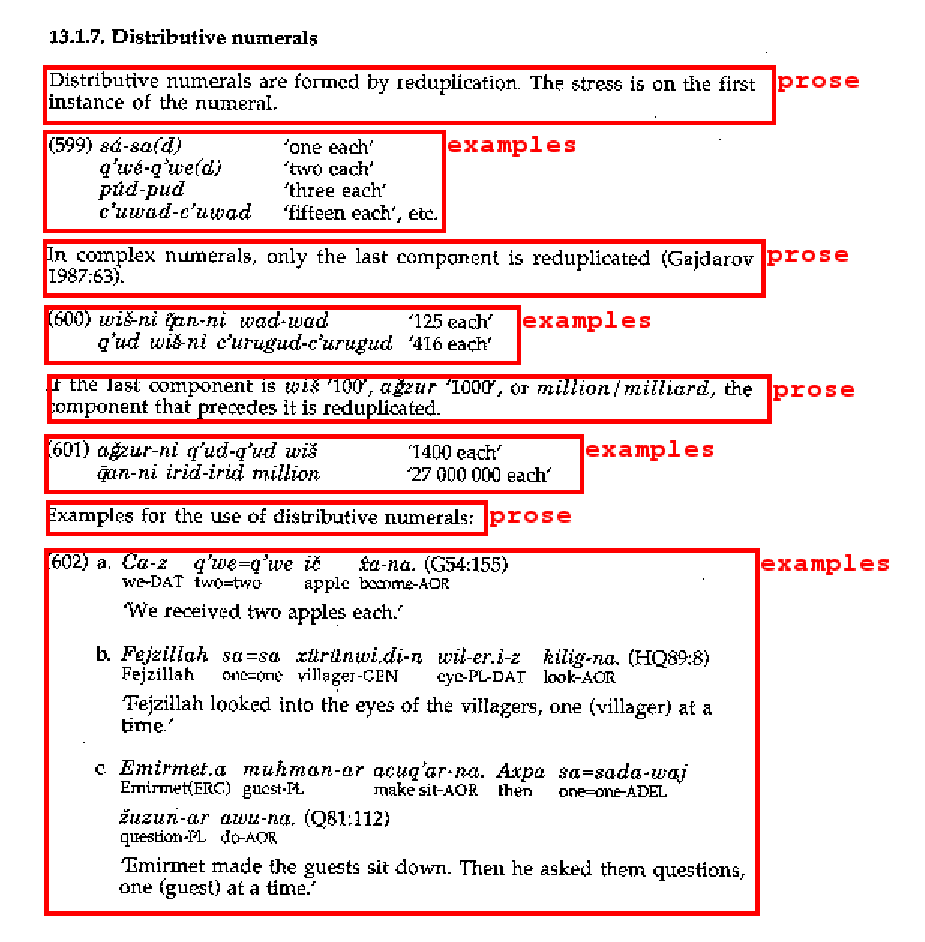
\includegraphics[width=\textwidth]{\imgpath/lezgian} 
\caption{The discussion of the distributive numerals in \citet{Haspelmath1993}}
\label{fig:lezgian}
\end{figure}


In Figure \ref{fig:lezgian}, the discussion is made up of prose, which is found before and after examples in a particular format which are use to illustrate the topic at hand, distributive numerals in this case. As a first step in structuring the text, we can separate the examples from the prose which discusses them \citep[cf.][]{Good2004}. The internal structure of the examples can then be worked out, as done for instance in \citet{BowEtAl2003}. The prose part has received less attention overall, which is why I will focus on this aspect here, next to the whole overarching structure of the book.

% In order to appreciate the internal diversity of the genre, a short historical overview is needed.
% The first major current of grammatical description of lesser known languages was missionary linguistics. In order to preach to the heathens, one had to know their language. So practical grammars of these languages were produced by missionaries to be handed over to new missionaries. The academic interest in the study of foreign language rose with American Structuralism in the beginning of the 20th century. Boas, Sapir and Bloomfield took on the task to describe the native American languages. It was in this period that the idea of describing a language in its own terms gained popularity. This contrasts with the missionary grammars, which often followed a model based on Latin or Greek grammar.


\section{The structure of grammatical descriptions: an overview}
Taking a look at the table of contents of the books in the sample, we find a certain recurrent ordering in the topics discussed. I take these findings to be uncontroversial, so I give an abbreviated XML-notation right away.\footnote{The 
 actual ordering of the chapters in the mainmatter may differ \citep{Mosel2006craft}, but what it is important here is that they are discussed as part of the mainmatter; the actual internal ordering is less relevant, as will be discussed below.
}

\ea\label{xml:book:intro}
\begin{verbatim}
<book>
  <frontmatter>
    <tableofcontents/ >
    <listoftables/ >
    <listoffigures/ >
    <listofabbreviations/ >
    <acknowledgments> ...  </acknowledgments>
 </frontmatter>
  <mainmatter>
    <background> ... </background>
    <phonology> ... </phonology>
    <morphology> ... </morphology>
    <syntax> ... </syntax>
    <semantics> ... </semantics>
 </mainmatter>
 <backmatter>
  <references/>
  <wordlist/>
  <texts>
    <text id="story1"> ... </text>
    <text id="recipe3"> ... </text>
  </texts>
 </backmatter>
</book>
\end{verbatim}
\z

The nature, relevance and functions of front- and backmatter are similar to what we find in other kinds of scientific books \citep{Mosel2006craft} so that the need to discuss these parts in this paper is less urgent. I will focus on the parts of the mainmatter then.
% Sperberg-McQueen and Bernard 2002 on TEI of dictionary

\section{The structure of the mainnmatter}
\subsection{Background}
Grammatical descriptions typically contain a chapter on the sociohistorical background of the language \citep{Lehmann2002}. In that chapter, the history and current sociological and political situation of the speech community is discussed. Topics covered are genealogical affiliation, geographical and political distribution, demographic factors such as ethnicity, religion, occupation and institutional representation. This part of the mainmatter does not seem to exhibit particular strong recurring structure and it does not seem wise to impose too tight a skeleton on it, so that I will treat it as unstructured data here.

\subsection{Morphosyntax: form-meaning-pairs ordered according to form}
Departing from the order normally found of books, I will now first discuss morphosyntax before coming back to phonology -- which is normally the first thing to be discussed -- in a minute. Depending on the language at hand, the division between morphology and syntax can be clear or rather subtle. While in Latin, the distinction is easy in most cases, other languages, like Tamil for instance, present challenges to the analyzer when they have to decide whether a given item is a suffix, an enclitic or an independent particle. There are ongoing theoretical discussions in particular languages about whether there is a division between morphology and syntax, and where it would be located (See \citet{CulicoverEtAl2005} for an overview for the English facts, \citet{Lehmann2002} for the consequences for language description). In light of these facts, it does not seem wise to impose a division in the schema until the differences are sorted out. What morphological and syntactical analyses have in common is that there is a certain form X which is said to have a certain function F. Whether X is treated as belonging to the morphological domain or to the syntactic domain is not substantial here. As an example, we can take the English possessive marker \em 's\em. No matter the analysis, we can say that \em 's \em is used to encode possession, widely construed. This is to say we are dealing with a \em form-meaning-pair\em.  The form \em 's \em of the English language is paired with the meaning \em possession\em. In this paper,  I propose that most of the morphosyntax of a language can be treated as discussion of form-meaning-pairs (henceforth abbreviated as `fomp').\footnote{A 
 `fomp' is a subset of the `Annotation' element proposed by \citet{Good2004}. `Annotations' are broader and could be used for other domains as well. It is a topic for further research to determine the relations between the general superordinate `annotation' type and the subset of form-meaning-pairs on the one hand and other types of description used in grammars (e.g. phonology)  on the other hand.
} 
Form-meaning-pairs consist of a topic of the discussion, which is at the same time the lemma (the name if you want) of the discussion. This topic is discussed with the help of illustrative examples\footnote{It
 seems sensible to have a container to contain a collection of individual examples illustrating aspects of the same phenomenon each. \citet{Good2004} calls this container \texttt{$<$exSet$>$}. In line with the general use of full words in markup in this paper, I use \texttt{$<$examples$>$}, but the two terms can be subsituted for each other.
} 
and surrounding prose.\footnote{The
 prose has an internal structure as well, consisting of running text interspersed with some special elements like references, \trs{word}{gloss}-pairs, technical terms and references. Specialized markup for these elements and links to ontologies enhance the computational usability of the grammatical description \citep{FarrarEtAl2003,Good2004}. For reasons of space and in order not to clutter the examples with tags, I omit the markup around the mentioned elements.
} 
We can illustrate this with the following fragment:

\ea
\label{xml:fofomp:intro}
\begin{verbatim}
<fomp type="form-to-function" lemma="'s">
  <prose>
    The phrasal affix <form> 's" </form>  is used to
    code <meaning> possession </meaning>.
  </prose>
  <examples>
    <example> My friend's car </example>
  </examples>
   <prose>
     As we see in the example above, the affix
     attaches to the right edge of an NP, in this
     case <objectlanguage> My friend </objectlanguage>.
   </prose>
</fomp>
\end{verbatim}
\z
 

As a consequence of the bipartite nature of the form-meaning-pair, discussion of the sign can focus on the form part (signifiant) or on the meaning part (signifié) \citep{Lehmann2004funkt}. Figure \ref{fig:cahuilla} from \citet{Seiler1985} shows a neat separation between the discussion of formal properties and the discussion of functional uses. In the formal part on top, marked in red, allomorphs, a purely formal phenomenon, are discussed, while in the functional part on the bottom, marked in blue, the communicative situations where this morpheme can be used are explicated, in this case \textsc{wishes}.

\begin{figure}
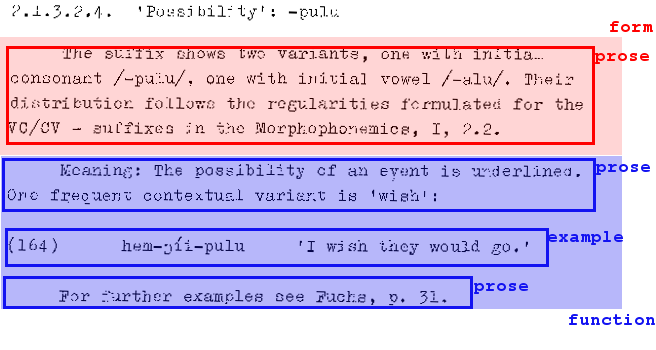
\includegraphics[width=\textwidth]{\imgpath/cahuilla} 
\caption{The discussion of the morpheme \em pulu- \em in \citet{Seiler1985}}
\label{fig:cahuilla}
\end{figure}


The division in a discussion of formal properties and functional properties can be squared with the alternation between prose and examples. Figure \ref{fig:hausa:ma} shows such a more complex configuration.

\begin{figure}
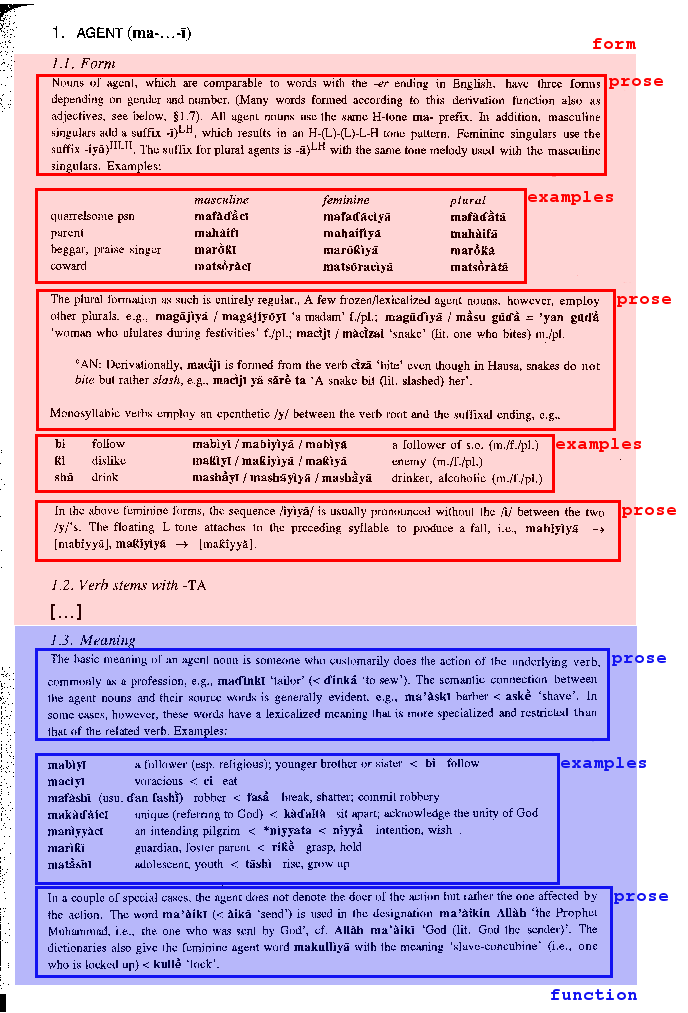
\includegraphics[height=\textheight]{\imgpath/hausa-agentma}
% hausa-agentma.png: 0x0 pixel, 0dpi, 0.00x0.00 cm, bb=
\caption{The discussion of the agentive morpheme \em ma- \em in \citet{Newman2000} shows a division of formal and functional properties, and a further subdivision in
\\
 prose parts and example parts.}
\label{fig:hausa:ma}
\end{figure}

This structure of the text can be represented in semantic markup \xref{xml:fofomp:functionalformal}.

\ea\label{xml:fofomp:functionalformal}
\begin{verbatim}
<fomp>
  <formaldescription>
    <prose>
      <form> XYX </form> has the following properties
    </prose>
    <examples>
      <example> ...</example>
    </examples>
  </formaldescription
  <functionaldescription>
    <prose>
      <form> XYX </form> is used for <meaning> Function
      FGH </meaning>
    </prose>
    <examples>
      <example> ...</example>
    </examples>
  </functionaldescription>
</fomp>
\end{verbatim}
\z


The kind of discussions we find in morphology have similarities to what we find in lexicography \citep{SchultzeBerndt1998,Mosel2006craft,Weber2006grow}. First the forms are enumerated, then the possible meanings are given; additional information about domain, register or etymology may also be provided. In light of the similarity to the lexicon, I will follow a suggestion by \citet{LehmannEtAl2004} and call the space where these things are discussed \em Morphemicon\em.

\subsection{Collections of fomps}
In grammtical descriptions, as in other books, related phenomena are often grouped together. Sentences which cover related ideas are grouped into a paragraph, related paragraphs into sections, and related sections into chapters, with possibly some intervening levels \citep{Good2004}. The conceptual unity of a discussion within a grammatical description is typically reflected in typography by white space. Tight coherence is mirrored by little space (e.g. between sentences), while more loose coherence is expressed by blank lines between paragraphs or blank pages between chapters. These organizational blocks thus reflect the semantic structure of the grammatical description. In a book, they are necessarily ordered linearly. However, when discussing the members of a set of morphemes, there is no inherent order. To take the French question words
\trs{qui}{who},
\trs{quand}{when},
\trs{quoi}{what},
\trs{comment}{how},
\trs{où}{where},
\trs{pourquoi}{why}, no clear order of discussion suggests itself. The discussion of \em qui \em is pretty much independent of the discussion of \em quand\em, and both are independent of the discussion of \em où\em. The gist of the description does not change if you discuss \em qui \em before \em quoi \em or the other way round. The fact that in grammatical descriptions they are found in the sections numbered X.1, X.2, X.3 etc is simply a reflex of the requirement of the linear structure for printing. These numberings correctly indicate the subordination of these concepts to a higher complex of `question words' (X in the example above), but they incorrectly suggest an inherent  order among these items.\footnote{\citet{Good2004} 
 concurs with the non-linear structure but remarks that the logical independence of these sections may be forfeited for a gain in didactic usefulness. To remain within the French example, the discussion of \em quoi \em should probably take place before \em pourquoi \em because the former is a component of the latter.
} 
When creating the semantic markup for grammatical descriptions, we should not be fooled by incidental side effects of printing. However, the hierarchical structure of grammatical descriptions must be recognized. Some phenomena need to be discussed at an abstract level.

To take an analogy from classical zoologic taxonomy, in the family of \em Felinae \em  we find the genera \em Lynx, Leopardus, Puma, \em and \em Felis\em, among others. There is surely no inherent order in discussing these genera, but some characteristics are shared among all members, e.g quadripedal, carnivore diet or moustaches. It would be redundant to state these facts at every individual level. They can better be discussed at the superordinate level of \em genus proximum\em. The same is true of linguistics. A semantic markup of grammatical description must provide for the possibility to state generalizations and sub/superordination. This is not a trivial problem. Here I would like to propose that this can be done by a general description followed by an enumeration of the members of the class with links to more detailed descriptions of the particular members. The XML-structure would be as follows:\footnote{For 
 reasons of simplicity, I omit the representation of `illustrative examples/paradigms' which are sometimes used in overview sections \citep{Good2004}.
}

\ea\label{xml:formlist}
\begin{verbatim}
<fomp type="formlist" name="Question words">
  <overview>
      <prose>
          Question normally start with the string "Wh".
          An exception is <form> how </form>. They are
          used to express <meaning> requests for
          information </meaning>. Question words normally
          trigger <form> do-support </form>.
      </prose>
  </overview>
  <ul>
    <li><form> Who </form></li>
    <li><form> What </form></li>
    <li><form> When </form></li>
    <li><form> Why </form></li>
    <li><form> Where </form></li>
    <li><form> How </form></li>
  </ul>
</fomp>
\end{verbatim}
\z

This list structure can be recursive \citep{Good2004}, so that deeper levels of subordination can be represented (free words$>$Nouns$>$Common Nouns$>$Count Nouns). Furthermore, multiple inheritance would also be possible.

As far as the treatment of formal (or semasiological) aspects is concerned, we thus have to distinguish two types of \textit{fomps}: a kind of  terminal node of the type ``form-to-function'' and a superordinate node of the type ``formlist''. The latter can include links to instances of the former.

The structure of the morphemicon can then be represented as in \xref{xml:morphemicon}. Note that the linear order of the elements is a coincidence here. The morphemicon is an \em un\em ordered list, as discussed above.\footnote{As
  an illustration of the unordered nature of fomps, we can take \citet{Newman2000}, who lists them in alphabetical order, the following is an excerpt from the table of contents:
  \begin{itemize}
  \item Prepositions
  \item Pro-Verb \em yi\em
  \item Pronouns
  \item Questions
  \item Reason and Purpose
  \item Reduplication
  \end{itemize}
}	

\ea\label{xml:morphemicon}
\begin{verbatim}
<morphemicon>
  <fomp type="formlist" name="Question words">
  ...
  </fomp>
  <fomp type="form-to-function" name="who">
  ...
  </fomp>
  <fomp type="form-to-function" name="what">
  ...
  </fomp>
  <fomp type="form-to-function" name="where">
  ...
  </fomp>
  <fomp type="form-to-function" name="why">
  ...
  </fomp>
  ...
  ...
  <fomp type="formlist" name="Demonstratives">
  ...
  </fomp>
  <fomp type="form-to-function" name="this">
  ...
  </fomp>
  <fomp type="form-to-function" name="that">
  ...
  </fomp>
</morphemicon>
\end{verbatim}
\z


\subsection{The treatment of examples: Bow, Hughes and Bird}

Besides the structure of the higher level elements and descriptive prose, the linguistic example is obviously central to the discussion of semantic markup. This area has received a seizable amount of research \citep{Drude2002,Peterson2002,BowEtAl2003}, which cannot be fully reviewed here. For the purposes of this paper, I adopt the XML-schema proposed by \citet{BowEtAl2003}, given for reference below.

\ea\label{xml:bbh}
\begin{verbatim}
<interlinear-text>
  <item type="title"> The Title</item>
  <phrases>
    <phrase>
      <item type="gls"> A phrasal translation</item>
      <words>
        <word>
          <item type="txt"> Word</item>
          <morphemes>
            <morph>
              <item type="txt"> Morph</item>
              <item type="gls"> Gloss</item>
            </morph>
            <morph>
              <item type="txt"> Morph</item>
              <item type="gls"> Gloss</item>
            </morph>
          </morphemes>
        </word>
      </words>
    <phrase>
  </phrases>
</interlinear-text>
\end{verbatim}
\z

This `raw' example can be further enhanced by information on meta-data (source, links to media files) and additional didactic annotations \citep[constituency, highlighting of important aspects][]{Good2004}.


\subsection{Extending formal description: beyond the morpheme}
In the paragraphs above I have discussed how morphemes can be linked to functions. However, morphemes are not the only meaning-bearing units in language. There are also constructions like \em VERB the TIME away \em e.g. \em dance/waltz/chat the night/evening away \em or more concrete \em kick the bucket \em \citep{CulicoverEtAl2005}. The particular meaning of these constructions is more than what is present in their morphemic parts, so that we must assume some meaning stemming from the construction itself \citep{FillmoreEtAl1993CxG,Goldberg1995CxG,Croft2001rcg}. Another example is the difference between \em John has come \em and \em Has John come?\em. In this case, the relative order of auxiliary and subject indicates whether we are dealing with an assertion or a question. The meaning-bearing units of a language are thus not exclusively atomic, but they can be complex as well \citep{Lehmann1993}. Furthermore, they are not always concrete as in the case of morphemes or idioms but they can also be schematic as in the case of the inversion questions. All this warrants the creation of a space where to discuss the meanings carried by these constructions. Following \citet{Goldberg1995CxG} I call this space \em constructicon\em.

The morphemicon deals with atomic and concrete elements, while the constructicon deals with schematic elements, which may be abstract or concrete. Both have in common that they deal with segmental material. Yet another complex bearing meaning in language is intonation, which is suprasegmental. The change of falling to rising intonation in the pair \em Jim's mother has come. \em vs. \em Jim's mother has come? \em has a predictable 	correspondence on the meaning side, the change of an assertion into a question. It seems best to treat intonation separated both from morphemes and constructions in a \em contouricon \em although there are of course some relations (WH-words trigger question intonation etc). The final structure of the morphosyntactic part is then

\ea\label{xml:semasiology}
\begin{verbatim} 
<forms>
 <morphemicon>
  <fomp type="morpheme" lemma="XX"> ... </fomp>
  <fomp type="morpheme"  lemma="YY"> ... </fomp>
  ...
 </morphemicon>
 <constructicon>
  <fomp type="construction" lemma="A B-C"> ... </fomp>
  <fomp type="construction" lemma="DE=F H G"> ... </fomp>
  ...
 </constructicon>
 <contouricon>
  <fomp type="intonation" lemma="HHL"> ... </fomp>
  <fomp type="intonation" lemma="HLH"> ... </fomp>
  ...
 </contouricon>
</forms>
\end{verbatim} 
\z

\subsection{Phonology}
The phonological part of grammatical description is normally structured as follows.

\ea\label{xml:phonology}
\begin{verbatim} 
<phonology>
  <segments>
    <phonemechart/ >
    <vowels> ... </vowels>
    <consonants> ... </consonants>
  </segments>
  <phonotactics> ... </phonotactics>
  <stress> ... </stress>
  <!-- <intonation> ... </intonation> -->
\end{verbatim}
\z

As discussed above, I propose to treat intonation as something which does not merely distinguish meaning (like phonemes) but which carries a meaning of its own, more like morphemes \citep[cf.][]{Mosel2006craft}.  Therefore, it can be meaningfully treated in the context of form-meaning-pairs, and there is no need to repeat the information in the phonological parts (although there should obviously be links between the two). This is why this element is commented out in \xref{xml:phonology}.

The remaining content in the phonological domain belongs to the domain of `distinguishing meaning'. This cannot be discussed in the context of form-meaning-pairs. The schmematization of this part will be left as a topic for future research.
 
\subsection{Semantics: form-meaning-pairs ordered according to function}
Above, I have discussed the structures we find in form-meaning-pairs based on morphemes and other forms.  This approach is called the form-to-function or semasiological approach. Let's call this perspective form-based form-meaning-pairs, or \em fo-fomps \em for short. It is possible to take the converse approach, i.e. function-to-form or onomasiological \citep{Gabelentz1891,Jespersen1924}. This approach is the one which is generally relevant in typological work, although it is less prevalent in extant grammatical descriptions \citep{Lehmann1980,
Comrie1998,
Lehmann1998,Lehmann2004funkt,
SchultzeBerndt1998,
Cristofaro2006,
Mosel2006craft,
Payne2006,
Zaefferer2006}, a notable example being \citep{Willett1991}. Figure \ref{fig:Willett} shows the table of contents of Willet's description of Southeastern Tepehuan

\begin{figure}

\begin{tabular}{ll}
  \begin{tabular}{ll}
  1 & Introduction\\
  2 & Phonology \\
  3 & Clause structure\\
  4 & Situations\\
  \hspace{.2cm}4.1 &Static situations \\
  \hspace{.2cm}4.2.& Dynamic situations \\
  5 & Entities\\
  6 & Settings\\
  \hspace{.2cm}6.1. & Location and direction\\
  \hspace{.2cm}6.2. & Time\\
  \hspace{.2cm}6.3. & Manner \\
  7 & Tense\\
\\
\\
\\
  \end{tabular}
  &
  \begin{tabular}{ll}
  8 & Aspect\\
  \hspace{.2cm}8.1 & Inception, termination and realization\\
  \hspace{.2cm}8.2 & Distinctiveness and simplicity \\
  \hspace{.2cm}8.3 & Resultative\\
  \hspace{.2cm}8.4 & Distribution, repetition and extent\\
  \hspace{.2cm}8.5 & Temporary and durative\\
  \hspace{.2cm}8.6 & Motion and transfer\\
  9 & Modality\\
  10 & Valence\\
  11 & Deixis\\
  12 & Specification\\
  13 & Coordination\\
  14 & Subordination\\
  15 & Continuity\\
  16 & Conclusion\\
  \end{tabular}
\end{tabular}
\caption{Excerpt from the table of contents of \citet{Willett1991}. For reasons of space, only selected subsections are shown.}
\label{fig:Willett}
\end{figure}


This is in many ways the mirror image of the former approach. Instead of taking a form and looking at the meanings it can express or the functions it can fulfill, we take a function and look at the forms it can be instantiated by. Let's call this perspective function-based form-meaning-pairs or \em fu-fomp\em. The division in prose parts and lists of examples is the same as above.

An illustrative example of the structure of a fu-fomp is given below in \xref{xml:fufomp:intro}. Note the similarity to example \xref{xml:fofomp:intro} above.

\ea\label{xml:fufomp:intro}
\begin{verbatim}
<fomp type="function-to-form" lemma="Comparison">
  <prose>
    The <function> comparative degree </function> of
    adjectives can be expressed by the suffix <form>
    -er </form> or by the particle <form> more </more>
  </prose>
  <examples>
    <example> Mary is taller than John </example>
    <example> Mary is more intelligent than
    John </example>
  </examples>
  <prose>
    As we see in the example above, short adjectives
    form the comparative with <objectlanguage>
    -er </objectlanguage> while longer adjectives take
    the particle <objectlanguage> more </objectlanguage>.
  </prose>
</fomp>
\end{verbatim}
\z




A more real-life example is given in Figure \ref{fig:lakota}, which shows the discussion of the function of comparison of adjectives in Lakota. This function can be instantiated by three different constructions. After an initial overview of what this section is about, three different constructions which can be used to convey this meaning are discussed. These are a) an adverb meaning `more', b) several other types of words with a rough meaning of `surpass' and finally c) a contrastive juxtaposition of the type `X is good and Y is bad'.

\begin{figure}
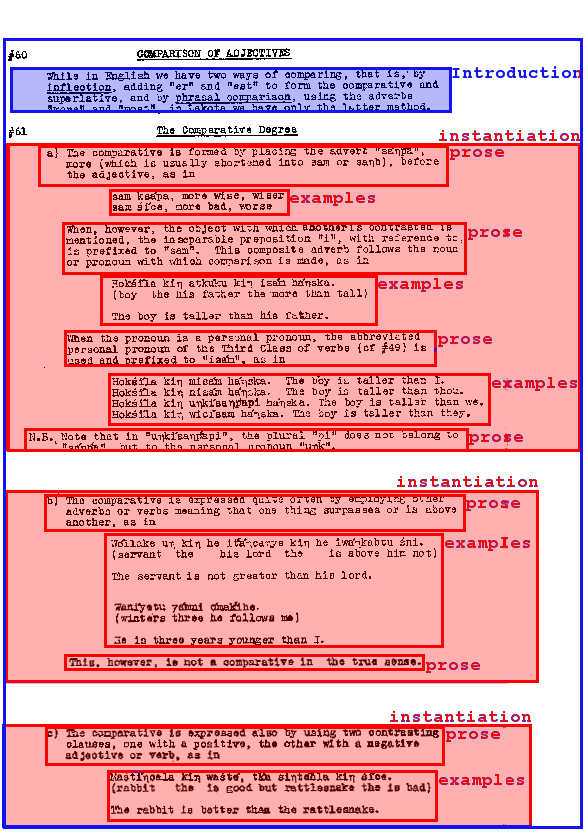
\includegraphics[height=\textheight]{\imgpath/lakota}
% lakota.png: 1179666x1179666 pixel, 0dpi, infxinf cm, bb=
\caption{The discussion of the function `Comparison of Adjectives' in Lakota in \citet{Buechel1939}, with three forms instantiating this function.}
\label{fig:lakota}
\end{figure}

Given that the readers of grammatical descriptions are normally expected to have a basic knowledge of the world, the introductory portions of fu-fomps tend to be short. There is no need to belabour the intended meaning of the function called `comparative degree' or `temporal reference prior to speech act' as this is pretty much self-evident from the naming. In some more involved domains involving less familiar concepts like e.g. the paucal, the introduction can be longer and illustrate the functional domain at hand in more detail. This is especially true for semantic distinctions presumed unfamiliar to the average reader, like alienability, evidentials, or the paucal mentioned above.

In a function-to-form approach, additional contrastive information can be provided about shades of meaning, frequency or register. This information is less commonly found in form-to-function approaches. Figure \ref{fig:tepehuan} from \citet{Willett1991} shows the description of a function and two formal instantiations thereof. Crucially, the two formal strategies come from different domains: the first one is a prefix (morphology) while the second one is a particle (syntax). In a form-to-function approach, the functional relatedness of these forms would have been difficult to convey. Furthermore, the two strategies can now be compared as to their felicity in different contexts, and their overall frequency. Without the functional \em tertium comparationis \em of `Intention' spelled out, this information would have been very difficult to find in the grammar.

\begin{sidewaysfigure}
 \centering
 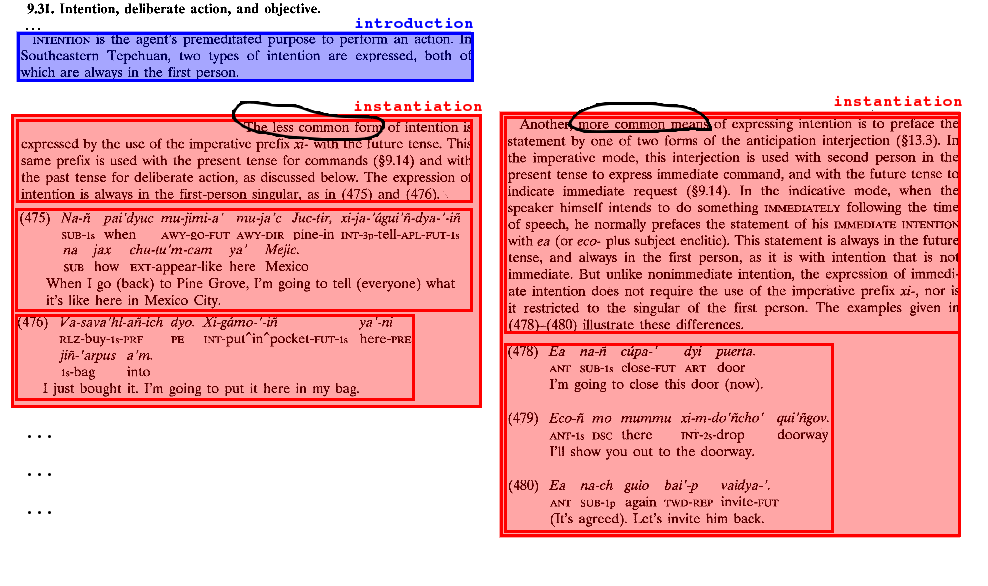
\includegraphics[width=\textwidth]{\imgpath/tepehuan.png} 
 \caption{A function-to-form description of `Intention' in Tepehuan \citep{Willett1991}.}
 \label{fig:tepehuan}
\end{sidewaysfigure}



\subsection{Extending functional description}
I have shown above that different types of fo-fomps exist, namely those which belong to the morphemicon, the constructicon, and the contouricon. In what concerns fu-fomps, a similar division exists. We can distinguish meaning components which are purely semantic and relate to the communicated content. Examples are participants, events, space, and time as in \em John ate a cake at the party at midnight\em. These meaning components can be grouped in a \em semanticon\em. This purely semantic information is different from meaning components like topic and focus, which do not belong to the propositional content. An example would be the difference between \em John came \em and \em It was John who came\em. These sentences communicate the same semantic content and are truth-equivalent. Yet, there is a difference in information structure in that in the second sentence, the hearer is already expected to know that an act of coming occurred, which is not the case in the first sentence. These components of meaning which belong to information structure or discourse pragmatics can be discussed in a \em discoursicon\em. Speech acts are yet another type of function which is outside of both semantics proper and discourse. An example would be a request like \em Please do come, John\em. I will collect this interpersonal type of information in a \em pragmaticon\em. This division mirrors the layered structure of the clause as found in a number of contemporary grammatical theories like Role \& Reference Grammar  \citep{FoleyEtAl1984,VanValinEtAl1997rrg} or Functional Grammar \citep{Hengeveld1989,HengeveldEtAl2008fdg}. We can add this structure to the general outline of grammatical descriptions \xref{xml:fufofomp}.
\ea\label{xml:fufofomp}
\begin{verbatim} 
<forms>
 <morphemicon>
  <fomp type="morpheme" lemma="ab"> ... </fomp>
  <fomp type="morpheme"  lemma="def"> ... </fomp>
 </morphemicon>
 <constructicon>
  <fomp type="construction" lemma="A B-C"> ... </fomp>
  <fomp type="construction" lemma="DE=F H G"> ... </fomp>
 </constructicon>
 <contouricon>
  <fomp type="intonation" lemma="HHL"> ... </fomp>
  <fomp type="intonation" lemma="HLH"> ... </fomp>
 </contouricon>
</forms>
<functions>
 <semanticon>
  <fomp type="semantics" lemma="space"> ... </fomp>
  <fomp type="semantics"  lemma="kin"> ... </fomp>
 </semanticon>
 <discoursicon>
  <fomp type="discourse" lemma="argument focus"> ... </fomp>
  <fomp type="discourse" lemma="new topic"> ... </fomp>
 </discoursicon>
 <pragmaticon>
  <fomp type="pragmatics" lemma="requests"> ... </fomp>
  <fomp type="pragmatics" lemma="insults"> ... </fomp>
 </contouricon>
<pragmaticon>
\end{verbatim} 
\z

A more extensive subdivision into 13 subcategories of meaning can be found in \citet{Lehmann2004docu}.\footnote{Apprehension 
 and nomination, concept modification, quantification, reference, possession, space construction, predication, design of situations, temporal orientation, illocution and modality, contrasting, nexion, articulation of discourse
}  
These subcategories can be partitioned among the semanticon, discoursicon and pragmaticon, which will not be formalized here.


\subsection{Collections of fu-fomps}
Like fo-fomps in \xref{xml:formlist}, fu-fomps can also be arranged hierarchically, for instance the hierarchy

\ea Expressing time $>$ Expressing internal temporal structure $>$ Expressing imperfective aspect. \z

One can state general observations at the higher levels of the hierarchy ("Tense and aspect are nearly always expressed by prefixes") and more particular observations lower down in the hierarchy ("Progressive aspect can be expressed by \em papu- \em or by \em pipo-\em")

\ea\label{xml:funclist}
\begin{verbatim}
<fomp type="funclist" name="Expressing time">
  <overview>
      <prose>
          Expressions of time cover lexical solutions
          like <objectlanguage> aujourd'hui </objectlanguage>
          <gloss> today </gloss> or <objectlanguage>
          hier </objectlanguage> <gloss> yesterday </gloss>.
          When time is expressed by bound morphemes, these
          are normally <form> suffixes<form>. This is true
          for both tense and aspect.
      </prose>
  </overview>
  <ul>
    <li><meaning> Expressing tense  </meaning></li>
    <li><meaning> Expressing aspect </meaning></li>
  </ul>
</fomp>
\end{verbatim}
\z

What has been said above about collections of fo-fomps applies \em mutatis mutandis \em to collections of fu-fomps as well.


\subsection{Interaction of fo-fomp and fu-fomp}
\citet{Mosel2006craft} notes that an ideal grammatical description could actually be required to state everything twice: once from a formal perspective and again from a functional perspective. A recent grammar which does precisely that is \citet{Nordhoff2009phd}. The table of contents for the formal and the functional part are given in figure \ref{fig:nordhoff}.

\begin{figure}
\parbox[t]{6cm}{
 Verbs\\
 Nouns\\
 Adjectives\\
 Adverbs\\
 Copula\\
 Personal pronouns\\
 Interrogative pronouns\\
 Deictics\\
 Quantifiers\\
 Numerals\\
 Interjections\\
 Modal particles\\
 Negative particles\\
 Other particles\\
 Conjunctions\\
 Classifiers\\ 
 Affixes\\
 Simple clitics\\
 Bound words\\
 Nominal and verbal morphology\\
 Verbal predicates\\
 Existential predicate\\
 Modal predicate\\
 Nominal predicates\\
 Circumstantial predicate\\
 Adjectival predicate \\
 Noun phrases\\  
 Postpositional phrases\\
 Main clauses\\
 Relative clause\\
 Conjunctive participle clause\\
 Purposive clauses\\
 Subordinate interrogative clauses\\
 Supraordination\\
 The position of adjuncts\\
 Reported speech\\
 Agreement\\
}
\parbox[t]{6cm}{
Particpants\\
Participants of different entity orders \\
.\hspace{.5cm}Participant roles \\
% Mismatches between number of semantic roles and number of syntactic arguments \\
.\hspace{.5cm}Unknown participants \\
.\hspace{.5cm}Modifying participants \\
Predication\\
.\hspace{.5cm}States \\
.\hspace{.5cm}Events \\
.\hspace{.5cm}Causation \\
% Giving extra information beyond the nuclear predication\\
Modification\\
Space\\
.\hspace{.5cm}Figure-ground relations \\
.\hspace{.5cm}Indicating   spatial orientation  \\
Time\\
.\hspace{.5cm}Figure and ground \\
.\hspace{.5cm}Phasal information \\
.\hspace{.5cm}Aspectual structure \\
Quantification\\
% Quantification of referents \\
% Event quantification \\
% Temporal frequency \\
Modality\\
Conditionals\\
Gradation\\
% Equation \\
% Similarity \\
% Superiority \\
% Inferiority \\
% Superlative \\
% Elative \\
% Abundantive \\
% Caritive \\
% Correlative \\
Comparison\\
Possession\\
.\hspace{.5cm}Assertion of the possessee \\
.\hspace{.5cm}Possession of abstract concepts \\
.\hspace{.5cm}Assertion of the possessor \\
% Presupposition of the possessor and the possessee \\
Negation\\
Kin\\
Referents and reference\\
Topic\\
Presupposition and assertion\\
Canceling implicatures\\
Parsing\\
Speech acts\\
Blending in the social tissue\\
}
\caption{The formal (left) and functional (right) table of contents of Nordhoff's grammar of Upcountry Sri Lanka Malay.}
\label{fig:nordhoff}
\end{figure}
 
The diligent reader will have noticed that the fo-fomp in example \xref{xml:fofomp:intro} and the fu-fomp in example \xref{xml:fufomp:intro} contain some additional markup. This markup can be used to link the form-to-function (semasiological) description with the function-to-form (onomasiological) description, a common desideratum for electronic grammars \citep{Comrie1998,Lehmann1998,Zaefferer1998,Mosel2006craft,Nordhoff2008jldc}. I will illustrate this with a fragment of the grammar of French, namely question formation.

In French, there exist three principal ways to request information from the hearer:  rising intonation contour, a question formative \em est-ce que\em,\footnote{For 
 the ease of discussion, I essentially treat \em est-ce que \em as unanalyzable here. It is true that this introducer can be segmented into \trs{est}{is}, \trs{ce}{this} and \trs{que}{that}, but the construction has grammaticalized to such an extent that there is little awareness of the internal constituency. This can also be seen from the fact that an authortitative reference grammar of French \citep{GrevisseEtAl1995} treats this construction as basically monomorphemic. The term `introducer' (`introducteur') is also taken from this work.
} 
and inversion. These three patterns are illustrated in \xref{ex:frenchquestions}. \xref{ex:frenchquestions:assertion} gives the declarative sentence for comparison.

\ea\label{ex:frenchquestions:assertion}
\gll Elle danse.\\
     She dances\\
    `She dances/is dancing'
\z
 
\ea\label{ex:frenchquestions}
\ea $\widetilde{\rm Elle}$ $\stackrel{\_\diagup\hspace{.7cm}}{\rm danse}$?
% \ea Elle $\widetilde{\rm danse}$?
\ex Est-ce qu'elle danse?
\ex Danse-t-elle?\\
 `Does she dance/Is she dancing?'
\z
\z

We see that there is a many-to-one relation form form to function, and a one-to many relation from form to function. We can illustrate this as in Figure \ref{fig:fufofomp:intro}.

\begin{figure}[h]
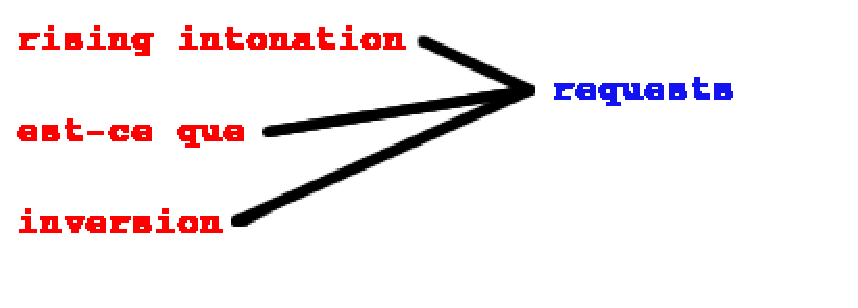
\includegraphics[width=.6\textwidth]{\imgpath/fufofomp0}
\caption{Many-to-one relations of form-meaning pairs}
\label{fig:fufofomp:intro} 
\end{figure}

At closer scrutiny, we find that inversion is used for other functions as well, for example with coordination as in \xref{ex:french:coordination}.

\ea\label{ex:french:coordination}
\gll ..., aussi chante-t-elle bien.\\
     {} also sing-link-she well\\
     `..., and also does she sing.'
\z

There is thus a many-to-many relation between form and function in language \citep{Noonan2006} as shown in Figure \ref{fig:fufofomp:outro}.
 

\begin{figure}[h]
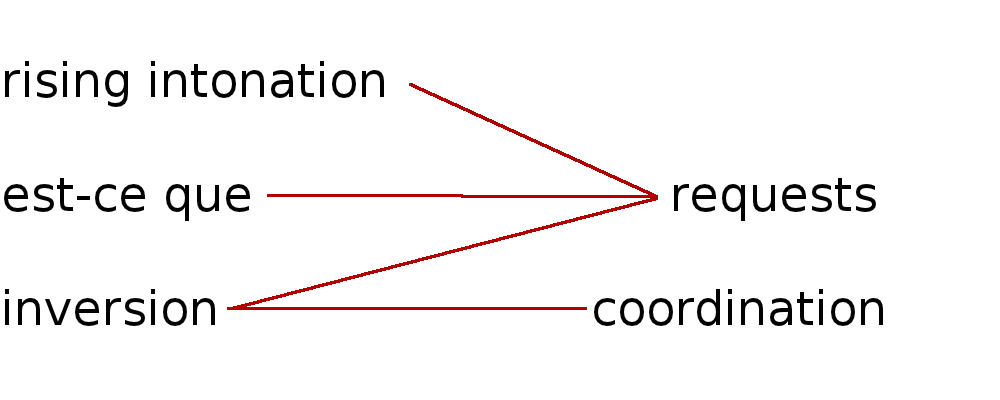
\includegraphics[width=.6\textwidth]{\imgpath/fufofomp}
\caption{Many-to-one relations of form-meaning pairs}
\label{fig:fufofomp:outro} 
\end{figure}

This relation can be expressed by a set of fo-fomps and fu-fomps as follows.\footnote{In 
 order to not complicate the example further, I dispense with the difference between universal conceptual categories like `question' and cross-linguistically common instantiations thereof, i.e. `interrogative sentence' \citep[but see][]{Lehmann1993}. This distinction is important and should be reflected in markup used for grammatical descriptions. However, in the context of this paper, it would incur too much theoretical overhead and would obscure the main line of argumentation. Future publications will explicate the relation in more detail than what can be covered here.
}

\ea\label{xml:french}
\begin{verbatim}
<fomp type="morpheme" lemma="est-ce que">
  <formaldescription>
    <prose>
      The introducer <form> est-ce que </form>  with
      the literal meaning <gloss> Is it so
      that ... ? </gloss>. In front of a following
      vowel, the form is <objectlanguage> est-ce
      qu'</objectlanguage>. Both forms are shown in
      the following examples.
    </prose>
    <examples>
      <example> [example with est-ce que]</example>
      <example> [example with est-ce qu']</example>
    </examples>
  </formaldescription>
  <functionaldescription>
    <form> Est-ce que </form> is used for <meaning>
    questions </meaning>
  </functionaldescription>
</fomp>

<fomp type="contour" lemma="H%">
  <formaldescription>
    <prose>
      The rising contour has a high tone target on the
      last syllable. 
    </prose>
    <examples>
      <example> [example with high tone target]</example>
    </examples>
  </formaldescription>
  <functionaldescription>
    This contour is used for <meaning> question
    formation </meaning>.
  </functionaldescription>
</fomp>

<fomp type="construction" lemma="Inversion">
  <formaldescription>
    <prose>
      In the <form> Inversion Construction</form>, the
      subject is repeated after the verb. Nominal subjects
      remain in front of the verb but pronominal subjects
      are deleted.
    </prose>
    <examples>
      <example> Marie danse-t-elle?</example>
      <example> (*Elle) Danse-t-elle?</example>
    </examples>
  </formaldescription>  
  <functionaldescription>  
    <prose>
      The <form> Inversion Construction</form> is used
      for <meaning> question formation </meaning> and
      for <meaning> coordination </meaning>.
    </prose>
    <examples>
      <example> Chante-t-elle? </example>
      <example> Aussi chante-t-elle bien </example>
    </examples>
  </functionaldescription>
</fomp>

<fomp type="Speechacts" lemma="Requests">
  <overview>
    <prose>
      A <meaning> request </meaning> is used to elicit
      information from the addressee.
    </prose>
  </overview>
  <instantiations>
    <prose>
      Three strategies
      can be used to form requests. These are <form>
      rising intonation </form>, <form> preposing the
      introducer <objectlanguage> est-ce
      que </objectlanguage></form>, and <form>
      inversion</form>.
    </prose>
    <examples>
      <example>  Elle danse?</example>
      <example>  Est-ce qu'elle danse danse?</example>
      <example>  Danse-t-elle?  </example>
    </examples>
    <prose>
      The first example is the least formal, the middle
      one is quite neutral, while the third one is decidedly
      formal and pertains to the written language.
    </prose>
  </instantiations>
</fomp>
\end{verbatim}
\z

This example models the many-to-many relations between form and function in a transparent way. The most relevant parts in the context of this discussion are \tag{form} \tag{/form} and \tag{meaning} \tag{/meaning}, which can be made to point to the page where the relevant formal or functional phenomenon is discussed in more detail. The reader might have noticed that the text between the tags varies and is not drawn from a restricted vocabulary. While there might be a possibility to avoid this arbitrariness in future descriptions, this is not possible when retrofitting the schema on extant descriptions. Therefore, the precise target of the form-links and the meaning-links has to be specified. So instead of

\ea \begin{verbatim}<form> preposing the introducer <objectlanguage> est-ce
que </objectlanguage></form>\end{verbatim} \z

we should have something like

\ea \begin{verbatim}<form target="est-ce que"> preposing the introducer
<objectlanguage> est-ce que </objectlanguage></form>\end{verbatim} \z

Note that the target {\tt "est-ce que"} matches the lemma tag of \texttt{<fomp type="morpheme" lemma="est-ce que">}.

In the same vein, we can rewrite 

\ea \begin{verbatim}A <meaning> request </meaning> is used to elicit
 information from the addressee.\end{verbatim}\z

as
  
\ea \begin{verbatim}A <meaning target="Requests"> request </meaning> is used
to elicit information from the addressee.\end{verbatim}\z

These targets are ideally linked to an ontology to make the references clear and consistent and facilitate cross-linguistic searches \citep{FarrarEtAl2003}. This will not be pursued here for reasons of space, but see \citet{Good2004,Goodtv} for ideas how this can be done.

\section{Interaction with the user}
As \citet{Weber2006grow} remarks, grammatical descriptions are never finished. New insights are continuously gained.\footnote{See
 \citet{Comrie1998,Cristofaro2006,Mosel2006craft,Payne2006,Rice2006} and \citet{Zaefferer2006} for similar observations.
} 
When a grammatical description is made available electronically, the findings can be updated.   \citet{Nordhoff2008jldc} discusses the  advantages of  and requirements for electronic grammar writing. An aspect not discussed in \citet{Nordhoff2008jldc} is the possibility for users to add tags to pages of an electronic description. These tags can be either arbitrary like \texttt{Compound}, \texttt{Important}, \texttt{SimilarToWarlpiri}, \texttt{Grammaticalization} or \texttt{V-Movement}. This kind of tag would have to be distinguished from a set of tags drawn from a closed restricted vocabulary. One possibility would be to rely on established schemas like the LDS questionnaire, so that tags like  \texttt{LDS\_2.3.4}  would have a clear and defined meaning. Another obvious provider for a restricted and controlled set of vocabulary would be the GOLD ontology \citep{FarrarEtAl2003}. If grammatical descriptions manage to draw a critical mass of tagging users, tag clouds can give a quick overview of the aspects of a certain page which the majority of the users find particularly relevant \citep[cf][]{BoudaEtAl2012ldl}.

\begin{figure}
 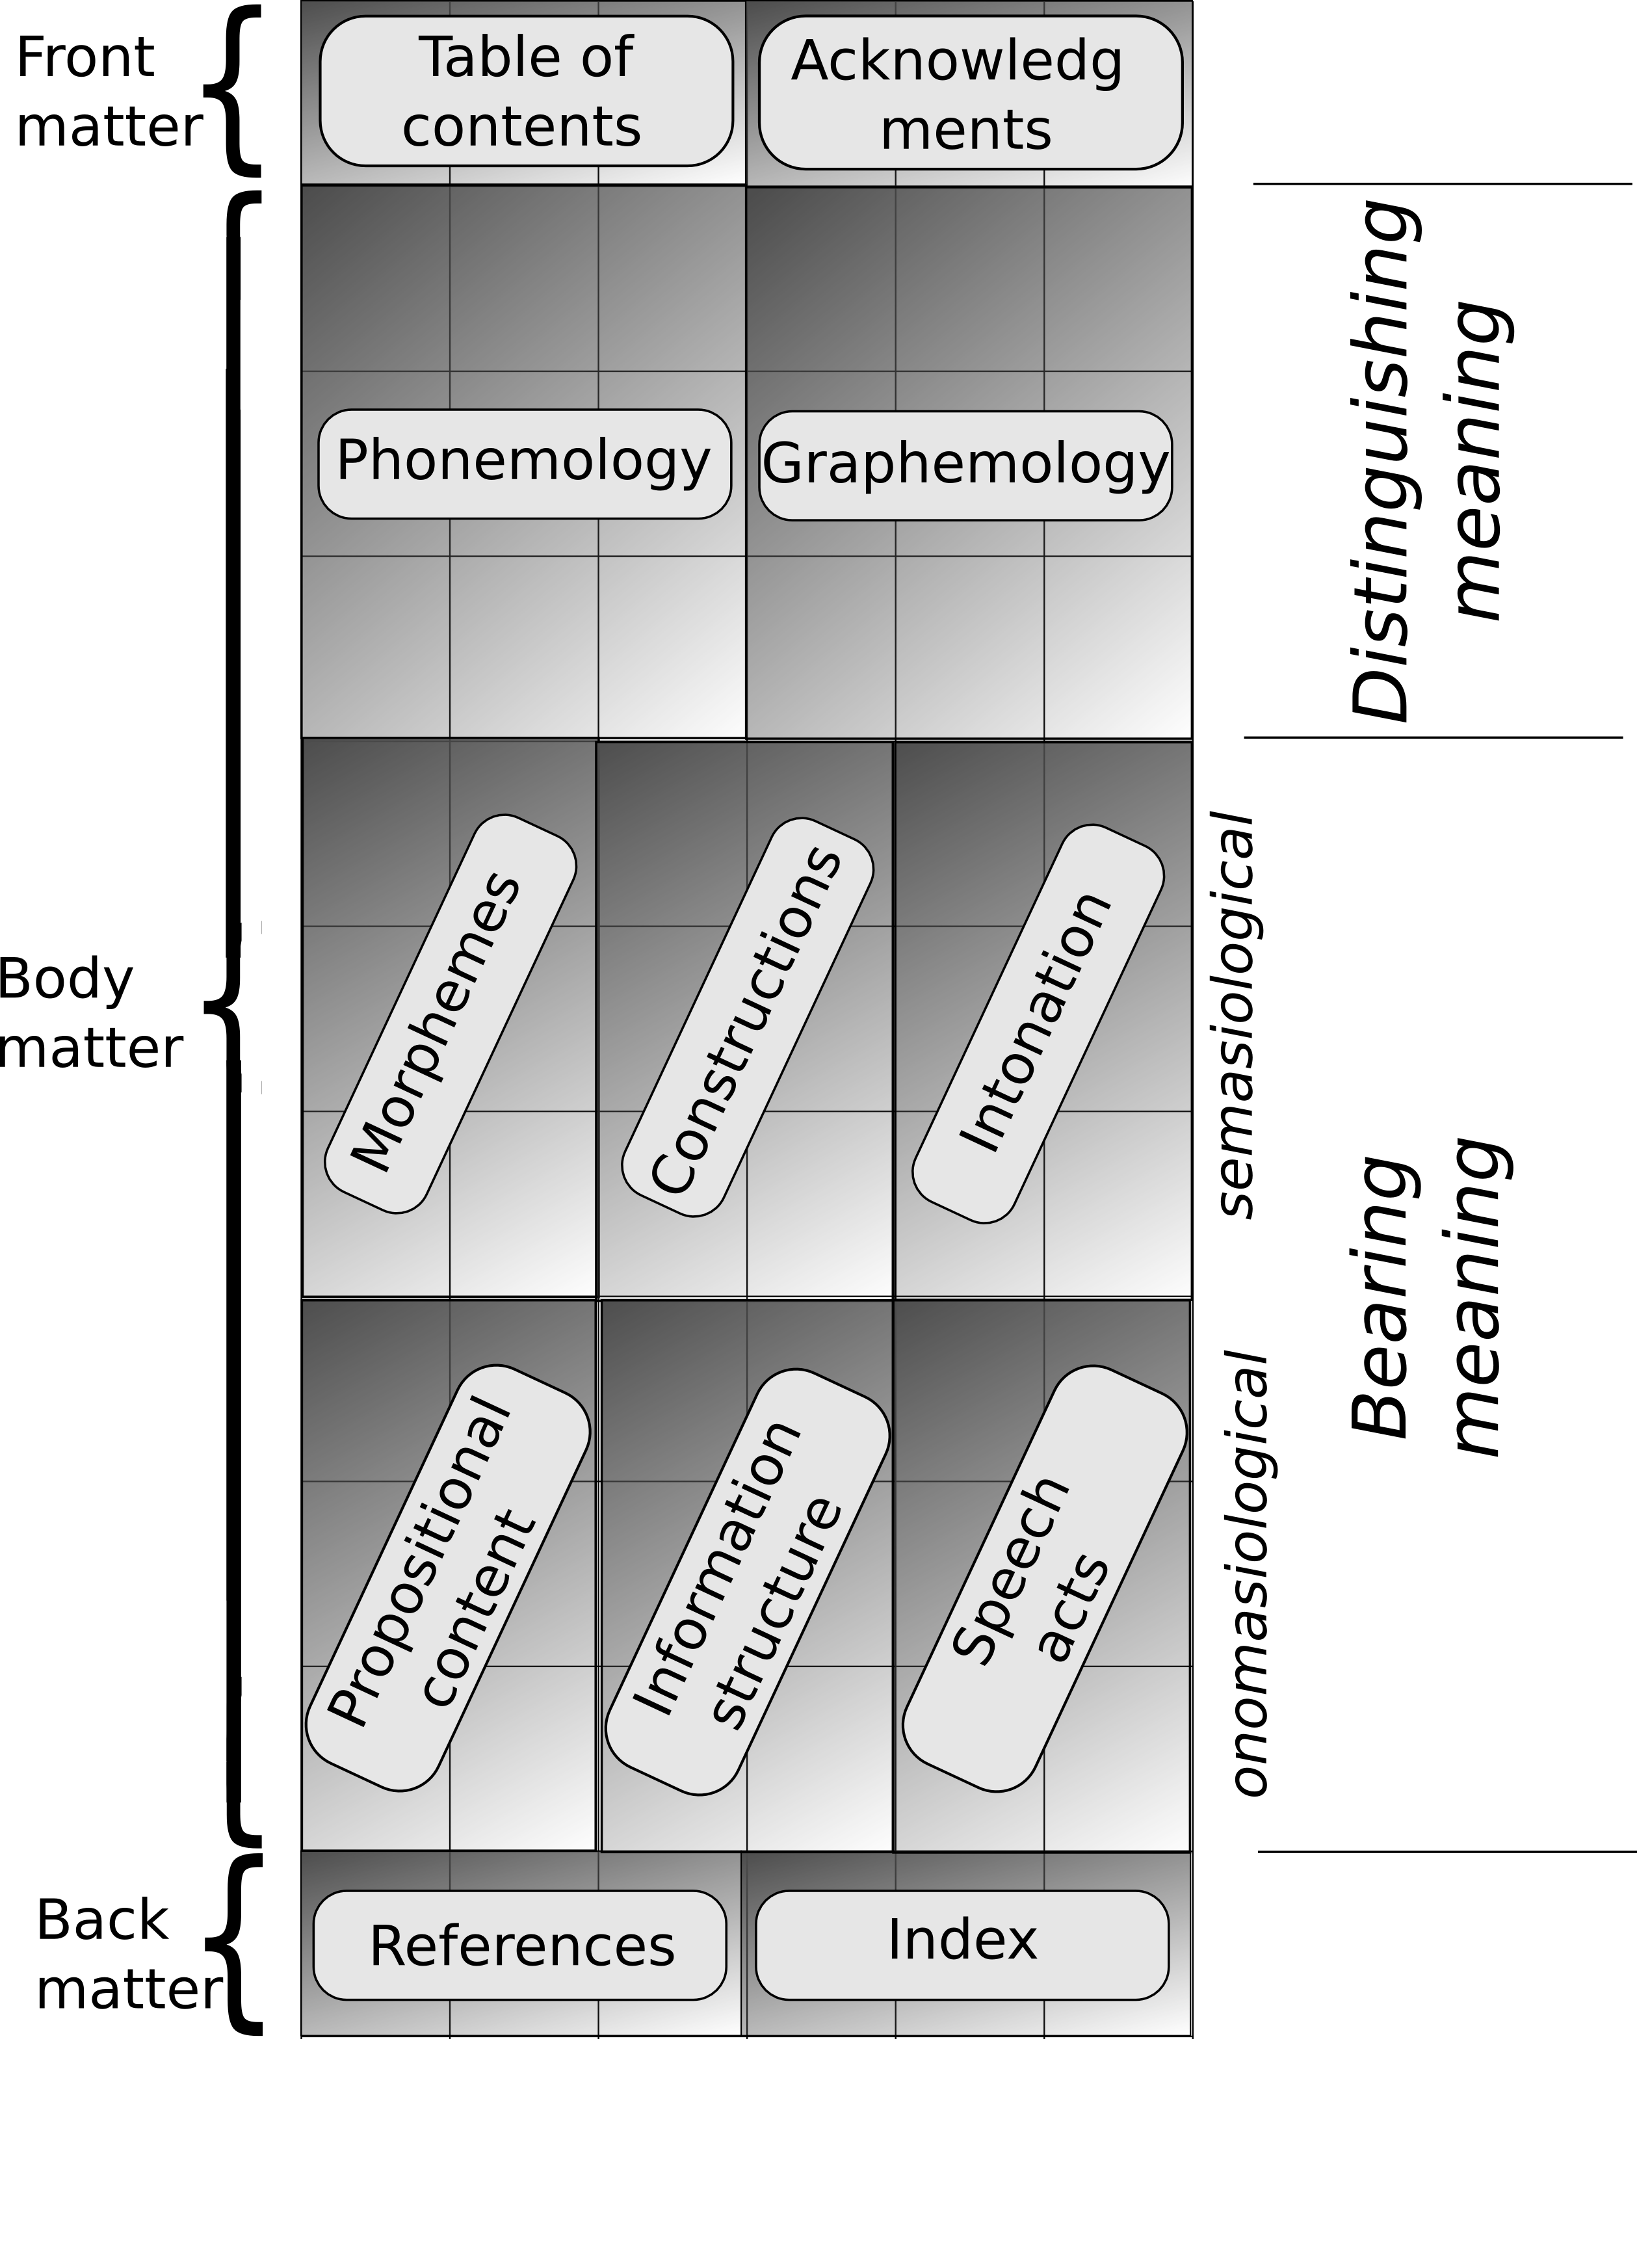
\includegraphics[width=\textwidth]{\imgpath/boxchart.png}
\caption{Visual illustration of the schema of grammatical descriptions.}
\label{fig:boxchart}
\end{figure}

\section{Schematization}
I have discussed the overall structure of a grammatical description above, including frontmatter, mainmatter and backmatter. The mainmatter was analyzed as consisting of a background part, a part for segmental phonology and two interdependent collections of form-meaning-pairs (`fomps'). The first one is based on the form-to-function or semasiological approach to grammatical analysis, while the second takes the converse onomasiological approach, function-to-form. The form-based and function-based fomps show similar structure. Both consist of alternating parts of prose and examples (Figure \ref{fig:boxchart}). These findings can be described in the RelaxNG schema given below (parts irrelevant in the context of this paper are treated as unstructured "texts" to keep the size of the schema within bounds).
\newpage
\footnotesize
\ea
\begin{verbatim}
GD =  element gd { Frontmatter,Mainmatter,Backmatter }
Frontmatter = element frontmatter { TOC, LOF, LOT, LOA, Acknowledgments }
Backmatter = element backmatter { References,Index }
Mainmatter = element mainmatter { Phonemology, Semasiology, Onomasiology }

Phonemology = element phonemology { Phonemicon }
Semasiology = element semasiology { Contouricon, Morphemicon, Constructicon }
Onomasiology = element onomasiology { Semanticon, Discoursicon, Pragmaticon }   

Phonemicon = element phonemicon  { text }
Contouricon = element contouricon  { Fo-Part }
Morphemicon = element morphemicon  { Fo-Part }
Constructicon = element constructicon  { Fo-Part }        

Semanticon = element semanticon  { Fu-Part } 
Discoursicon = element discoursicon { Fu-Part } 
Pragmaticon = element pragmaticon { Fu-Part }

Fo-Part = element fo-collection { (Fo-Collection|Fo-Fomp)* }
Fo-Collection = element fo-list { Tags,  Prose, Examples, Formlinklist }

Fu-Part = element fu-collection { (Fu-Collection|Fu-Fomp)* }
Fu-Collection = element fu-list { Tags,  Prose, Examples, Funclinklist }

Examples = element examples { Example+ }
 
Fo-Fomp = element fo-fomp { Tags,  Overview, Formaldescription, Functionaldescription }
Formaldescription = element formaldescription { (Prose|Example)* }
Functionaldescription = element functionaldescription { (Prose|Example)* }

Fu-Fomp = element fu-fomp { Tags,  Overview, Instantiations }
Instantiations = element instantiations { (Prose|Example)* }

Overview = element overview { text }
Prose = element prose { text }

Example = element example { Tags,  Bowhughesbird }
Bowhughesbird = element bowhughesbird { text }

Formlinklist = element formlinklist  { Formlink+ }
Funclinklist = element funclinklist  { Funclink+ }

Formlink = Link
Funclink = Link

Link = element link { attribute name { text }, attribute target { text } }
Tags = element tag { attribute name { text } }*

TOT = element tableofcontents { text }
LOF = element listoffigures { text }
LOT = element listoftables { text }
LOA = element listofabbreviations { text }
Acknowledgments = element acknowledgments { text }
References = element references { text }
Index = element index { text }

\end{verbatim}
\z
\normalsize

\section{Conclusion and outlook}
This paper has analyzed the semantic structure of grammatical descriptions and shown that in the domain of form-meaning pairs,  the interaction between the  semasiological and the onomasiological approach  can be formalized in a RelaxNG schema. Grammars structured along this schema have a number of advantages. First, the schema encourages encapsulation of the descriptive content. The descriptive content in each fomp should be independent of the surrounding fomps. If the schema is adhered to, the constraint of linearity disappears. The elements are self-contained, which allows for addition and modification of elements without affecting the overall structure (terminological consistency remains an issue of course). This means that grammars can be written and published in an incremental heap-like way, making new insights available to the general public as they are gained \citep[cf.][]{Weber2006grow,Goodtv}. Furthermore, the basic advantages of structured text obtain, e.g. semantic searches, extraction, modification, differential presentation \citep{Maxwelltv}.

The schema proposed here is designed to be compatible with recent structuring proposals in other domains of grammar, namely \citet{BowEtAl2003} and \citet{Good2004}. Further work in analyzing the structure of grammatical descriptions needs to be done. Issues for further theoretical work are: the structure of phonological descriptions, the nature of tags and links, and the implementation of a controlled vocabulary for certain fields through an ontology. As far as practical applications are concerned, the schema will have to be measured against the actual requirements of future and past grammars. Is it possible to use this schema when writing a grammar, and is it possible to retrofit this schema on an existing grammar? As for the former question, first results are positive. \citet{Nordhoff2009phd} is a descriptive grammar of a previously undescribed language, Sri Lanka Malay. While this grammar is not in XML-format yet, it was designed with the application of the above schema in mind. As such it contains a formal part and a functional part, which are roughly structured as outlined above. Furthermore, the individual sections in the two parts are parallel to fo-fomps and fu-fomps. The conversion process of the manuscript to XML is currently under way and looks promising. Retrofitting the schema on legacy descriptions is a more difficult task. The book has to be split into independent fomps. Depending on whether the author adhered to a strict separation of formal and functional discussion \citep[e.g.][]{Seiler1985}, the task is more or less easy. Resolving interparagraph dependencies (\em as demonstrated in the last paragraph, as shown below, contrary to what was said in the preceding section \em etc) will probably be a problematic issue in splitting the grammatical description into independent chunks on which the schema can be applied. In a first step, retrofitting will be done manually, but in a second step, semi-automatic analysis of the structure of grammatical descriptions remains a goal. Extraction tools like \citet{Lewis2006} are probably a worthwhile domain to investigate for these prospects.

The ultimate goal would be to have an online repository of all existing grammatical descriptions which are converted to XML. These could be queried in a semantic fashion. The query would yield all the descriptive content of the selected grammars about a particular domain, a very useful feature for large sample typology. While there is still a very long way to go, the GALOES platform \citep{Nordhoff2007alt,Nordhoff2007dobes,Nordhoff2007mpi} is aimed at supporting language describers in writing XML-based grammars. Descriptive departments in several European countries have expressed interest in collaboration. In the long run, this should assure that future grammatical descriptions comply with the schema. As for legacy descriptions, the next step will be an analysis of the 10,000 electronic grammars collected by Harald Hammarstöm to see how far automatic extraction procedures can get us. This topic will be treated in future papers.  

% 
% \bibliographystyle{natuva}
% \bibliography{asw,grammaticography,grammars,nordhoff}
% 
% \section{Appendix}
% \footnotesize
% \begin{verbatim}<?xml version="1.0" encoding="UTF-8"?>
% <xs:schema xmlns:xs="http://www.w3.org/2001/XMLSchema" elementFormDefault="qualified">
%   <xs:element name="gd">
%     <xs:complexType>
%       <xs:sequence>
%         <xs:element ref="frontmatter"/>
%         <xs:element ref="mainmatter"/>
%         <xs:element ref="backmatter"/>
%       </xs:sequence>
%     </xs:complexType>
%   </xs:element>
%   <xs:element name="frontmatter">
%     <xs:complexType>
%       <xs:sequence>
%         <xs:element ref="tableofcontents"/>
%         <xs:element ref="listoffigures"/>
%         <xs:element ref="listoftables"/>
%         <xs:element ref="listofabbreviations"/>
%         <xs:element ref="acknowledgments"/>
%       </xs:sequence>
%     </xs:complexType>
%   </xs:element>
%   <xs:element name="backmatter">
%     <xs:complexType>
%       <xs:sequence>
%         <xs:element ref="references"/>
%         <xs:element ref="index"/>
%       </xs:sequence>
%     </xs:complexType>
%   </xs:element>
%   <xs:element name="mainmatter">
%     <xs:complexType>
%       <xs:sequence>
%         <xs:element ref="phonemology"/>
%         <xs:element ref="semasiology"/>
%         <xs:element ref="onomasiology"/>
%       </xs:sequence>
%     </xs:complexType>
%   </xs:element>
%   <xs:element name="phonemology" type="Phonemicon"/>
%   <xs:element name="semasiology">
%     <xs:complexType>
%       <xs:sequence>
%         <xs:element ref="contouricon"/>
%         <xs:element ref="morphemicon"/>
%         <xs:element ref="constructicon"/>
%       </xs:sequence>
%     </xs:complexType>
%   </xs:element>
%   <xs:element name="onomasiology">
%     <xs:complexType>
%       <xs:sequence>
%         <xs:element ref="semanticon"/>
%         <xs:element ref="discoursicon"/>
%         <xs:element ref="pragmaticon"/>
%       </xs:sequence>
%     </xs:complexType>
%   </xs:element>
%   <xs:complexType name="Phonemicon">
%     <xs:sequence>
%       <xs:element ref="phonemicon"/>
%     </xs:sequence>
%   </xs:complexType>
%   <xs:element name="phonemicon" type="xs:string"/>
%   <xs:element name="contouricon" type="Fo-Part"/>
%   <xs:element name="morphemicon" type="Fo-Part"/>
%   <xs:element name="constructicon" type="Fo-Part"/>
%   <xs:element name="semanticon" type="Fu-Part"/>
%   <xs:element name="discoursicon" type="Fu-Part"/>
%   <xs:element name="pragmaticon" type="Fu-Part"/>
%   <xs:complexType name="Fo-Part">
%     <xs:sequence>
%       <xs:element ref="fo-collection"/>
%     </xs:sequence>
%   </xs:complexType>
%   <xs:element name="fo-collection">
%     <xs:complexType>
%       <xs:choice minOccurs="0" maxOccurs="unbounded">
%         <xs:element ref="fo-list"/>
%         <xs:element ref="fo-fomp"/>
%       </xs:choice>
%     </xs:complexType>
%   </xs:element>
%   <xs:element name="fo-list">
%     <xs:complexType>
%       <xs:sequence>
%         <xs:group ref="Tags"/>
%         <xs:element ref="prose"/>
%         <xs:element ref="examples"/>
%         <xs:element ref="formlinklist"/>
%       </xs:sequence>
%     </xs:complexType>
%   </xs:element>
%   <xs:complexType name="Fu-Part">
%     <xs:sequence>
%       <xs:element ref="fu-collection"/>
%     </xs:sequence>
%   </xs:complexType>
%   <xs:element name="fu-collection">
%     <xs:complexType>
%       <xs:choice minOccurs="0" maxOccurs="unbounded">
%         <xs:element ref="fu-list"/>
%         <xs:element ref="fu-fomp"/>
%       </xs:choice>
%     </xs:complexType>
%   </xs:element>
%   <xs:element name="fu-list">
%     <xs:complexType>
%       <xs:sequence>
%         <xs:group ref="Tags"/>
%         <xs:element ref="prose"/>
%         <xs:element ref="examples"/>
%         <xs:element ref="funclinklist"/>
%       </xs:sequence>
%     </xs:complexType>
%   </xs:element>
%   <xs:element name="examples">
%     <xs:complexType>
%       <xs:sequence>
%         <xs:element maxOccurs="unbounded" ref="example"/>
%       </xs:sequence>
%     </xs:complexType>
%   </xs:element>
%   <xs:element name="fo-fomp">
%     <xs:complexType>
%       <xs:sequence>
%         <xs:group ref="Tags"/>
%         <xs:element ref="overview"/>
%         <xs:element ref="formaldescription"/>
%         <xs:element ref="functionaldescription"/>
%       </xs:sequence>
%     </xs:complexType>
%   </xs:element>
%   <xs:element name="formaldescription">
%     <xs:complexType>
%       <xs:choice minOccurs="0" maxOccurs="unbounded">
%         <xs:element ref="prose"/>
%         <xs:element ref="example"/>
%       </xs:choice>
%     </xs:complexType>
%   </xs:element>
%   <xs:element name="functionaldescription">
%     <xs:complexType>
%       <xs:choice minOccurs="0" maxOccurs="unbounded">
%         <xs:element ref="prose"/>
%         <xs:element ref="example"/>
%       </xs:choice>
%     </xs:complexType>
%   </xs:element>
%   <xs:element name="fu-fomp">
%     <xs:complexType>
%       <xs:sequence>
%         <xs:group ref="Tags"/>
%         <xs:element ref="overview"/>
%         <xs:element ref="instantiations"/>
%       </xs:sequence>
%     </xs:complexType>
%   </xs:element>
%   <xs:element name="instantiations">
%     <xs:complexType>
%       <xs:choice minOccurs="0" maxOccurs="unbounded">
%         <xs:element ref="prose"/>
%         <xs:element ref="example"/>
%       </xs:choice>
%     </xs:complexType>
%   </xs:element>
%   <xs:element name="overview" type="xs:string"/>
%   <xs:element name="prose" type="xs:string"/>
%   <xs:element name="example">
%     <xs:complexType>
%       <xs:sequence>
%         <xs:group ref="Tags"/>
%         <xs:element ref="bowhughesbird"/>
%       </xs:sequence>
%     </xs:complexType>
%   </xs:element>
%   <xs:element name="bowhughesbird" type="xs:string"/>
%   <xs:element name="formlinklist">
%     <xs:complexType>
%       <xs:group maxOccurs="unbounded" ref="Formlink"/>
%     </xs:complexType>
%   </xs:element>
%   <xs:element name="funclinklist">
%     <xs:complexType>
%       <xs:group maxOccurs="unbounded" ref="Funclink"/>
%     </xs:complexType>
%   </xs:element>
%   <xs:group name="Formlink">
%     <xs:sequence>
%       <xs:element ref="link"/>
%     </xs:sequence>
%   </xs:group>
%   <xs:group name="Funclink">
%     <xs:sequence>
%       <xs:element ref="link"/>
%     </xs:sequence>
%   </xs:group>
%   <xs:element name="link">
%     <xs:complexType>
%       <xs:attribute name="name" use="required"/>
%       <xs:attribute name="target" use="required"/>
%     </xs:complexType>
%   </xs:element>
%   <xs:group name="Tags">
%     <xs:sequence>
%       <xs:element minOccurs="0" maxOccurs="unbounded" ref="tag"/>
%     </xs:sequence>
%   </xs:group>
%   <xs:element name="tag">
%     <xs:complexType>
%       <xs:attribute name="name" use="required"/>
%     </xs:complexType>
%   </xs:element>
%   <xs:element name="tableofcontents" type="xs:string"/>
%   <xs:element name="listoffigures" type="xs:string"/>
%   <xs:element name="listoftables" type="xs:string"/>
%   <xs:element name="listofabbreviations" type="xs:string"/>
%   <xs:element name="acknowledgments" type="xs:string"/>
%   <xs:element name="references" type="xs:string"/>
%   <xs:element name="index" type="xs:string"/>
% </xs:schema>
% 
% \end{verbatim}
% 
% \normalsize
%  
\documentclass{article}
\usepackage[utf8]{inputenc} % please use UTF8 encoding
\usepackage[T1]{fontenc} 
\usepackage{gb4e}

\begin{document} 
% This file was converted to LaTeX by Writer2LaTeX ver. 1.0.2
% see http://writer2latex.sourceforge.net for more info
\documentclass[letterpaper]{article}
\usepackage[ascii]{inputenc}
\usepackage[T3,T1]{fontenc}
\usepackage[english]{babel}
\usepackage[noenc]{tipa}
\usepackage{tipx}
\usepackage{amsmath}
\usepackage{amssymb,amsfonts,textcomp}
\usepackage[top=0.4917in,bottom=0.7874in,left=0.9839in,right=0.9839in,includehead,head=0.4925in,headsep=0.4528in,nofoot]{geometry}
\usepackage{array} 
\usepackage{hhline}
\usepackage{hyperref}
\hypersetup{colorlinks=true, linkcolor=blue, citecolor=blue, filecolor=blue, urlcolor=blue}
\usepackage{graphicx}
\begin{document}
\clearpage\setcounter{page}{1}\pagestyle{Standard}

\end{document}


\end{document}


\glossSTDmode
\setcounter{exx}{0}\setcounter{footnote}{0}
\renewcommand{\imgpath}{./Thieberger}
\renewcommand{\thischapteruuheader}{\uhheader{63-77}{4530}}
\renewcommand\chapname{Hypertext for Nunggubuyu}
\renewcommand\longchapname{Language description and hypertext: Nunggubuyu as a case study}
\renewcommand\shortauthor{Simon Musgrave and  Nick Thieberger}
\renewcommand\longauthor{Simon Musgrave$^\spadesuit$ , Nick Thieberger$^\heartsuit$ \\
$^\spadesuit$Monash University, $^\heartsuit$University of Melbourne}
\chapter*{\longchapname}
\chapterauthor{\longauthor}
\mytoc{}


\begin{abstract}

Any reasonably complete description of a language is a complex object, typically composed of a grammar, a dictionary, and a text collection with internal relationships that can be represented as hyperlinks. The information would be fully searchable, links between text and media could be implemented, and the presentation would be based on a well-defined data structure with advantages for archiving and reusability. 

We present a small fragment from Heath's Nunggubuyu text collection with links to parts of the other elements of the description to demonstrate the benefit which this approach can bring. This initial step involves a certain amount of hand-coding but establishes a basis for the necessary data structure which will then be used in a second phase where we develop techniques for the automatic processing of scanned versions of Heath's work. 

Grammatical descriptions written with the kinds of structure we are developing, or capable of being converted to that structure (while being `born digital') are likely to be in short supply. Presentations of old materials in new formats will inform new electronic grammars, and help gain the acceptance of the linguistic community for preferred formats.

\end{abstract}


\section{Introduction}\label{thie:sec:1}
Any reasonably complete description of a language is a complex object. Traditionally, such works are divided into various components: a grammar, a dictionary and a text collection, the so-called Boasian trilogy. But of course these are really highly inter-related. For example, a single entry in the dictionary is of little value without the general information about words of that class which can be found in the grammar, and any point made in the grammar may be hard to grasp without extensive exemplification from texts. Boas himself was well aware of this fact:

\begin{quote}
  We have vocabularies; but, excepting the old missionary grammars, there is very little systematic work. Even where we have grammars, we have no bodies of aboriginal texts {\dots}. [I]t has become more and more evident that large masses of text are needed to elucidate the structure of the languages \citep[1]{Boas1917}
\end{quote}

As \citet[163]{Woodbury2011} comments on this passage: ``All three were interrelated parts of a documentary whole, treating, in different ways, overlapping empirical domains''.

The interrelatedness of the various components discussed above immediately suggests that hypertext would be a better means of presentation and additional benefits could come from making the grammatical description a multimedia object, rather than a text object. Examples could be heard in the original sound recorded by the researcher, or even seen as video clips where such presentation would aid the consumer (for example, where gesture added an important element of meaning to the utterance). In addition to the improved accessibility of the descriptive information, such presentation would bring the consumer much closer to the primary data, actual language in use, and therefore multimedia language description would increase substantially the standard of accountability in linguistics. However, the standard paper and ink presentation of grammatical description has an established linear format which is not suitable for the new medium. 

Most grammatical descriptions published in book format follow more or less closely a standard format. The presentation begins with background information on the language and its speakers, the relationship of the language to other languages, and a survey of previous research. The description proper then follows, moving through phonetics and phonology (the sounds of the language and how they are organized into a system), morphology (word-formation processes), and clausal syntax. Some discussion of syntax above the level of the individual clause and of textual organization may follow. If example texts are included in the volume, as is common, they will come after this, with word lists after them \citep{Nordhofftv}. The organization of a grammar in this style is linear, that is, one sort of information is presented before another. And the linearity is to a large extent well-motivated. It is generally not easy to understand the morphological processes of a language before one understands the phonology; it is hard to understand syntax (combinations of words) before one understands morphology (word-formation). Linearity of presentation is also a consequence of the medium. Paper and ink objects are read normally in sequence; even if one reads only a short section of a larger work, one starts at a particular place and reads on in sequence for as long as necessary. Hypertext, on the other hand, is a non-linear medium and the metaphor of a web is entirely appropriate for such presentation. As already mentioned, hypertext has clear benefits for the presentation of grammatical description, but it is desirable that at least some of the linear logic of the paper and ink model should be accessible in the new medium.

We wish to explore the possibilities of presenting grammatical description in an electronic form while maintaining a strong link with the traditional mode of presentation (cf Drude this volume). In order to do this, the ideal material to work with is a description presented in book format which nevertheless makes extensive use already of the interrelatedness of its various components. Jeffrey Heath's description of Nunngubuyu fits these criteria. The following section briefly describes this work and illustrates its value as an exemplar for developing richly interlinked language description for electronic presentation. Section~3 of this paper discusses our approach to encoding the source texts to make them accessible for online presentation and section~4 outlines our plans for further development of this project. Finally, in section~5, we turn to some design issues in electronic grammaticography as we view them in light of our work on Nunggubuyu. 

\section{Heath's Description of Nunggubuyu}
Nunggubuyu (ISO639-3: \texttt{nuy}, also known as Wubuy) is a non-Pama Nyungan language spoken in Arnhem Land, Australia (see Figure \ref{thi:fig:map1}).

\begin{figure} 
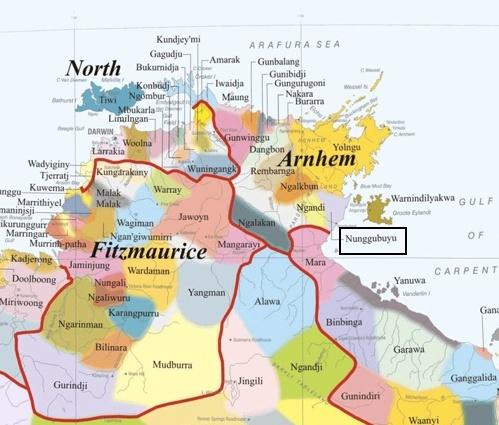
\includegraphics[width=\textwidth]{\imgpath/Thieberger2-img1.jpg}
\caption{Arnhem Land, showing the location of Nunggubuyu} 
\label{thi:fig:map1}
\end{figure}

Heath's description of the language was published in three volumes: texts \citep{Heath1980}, dictionary \citep{Heath1982} and grammar \citep{Heath1984}. The three volumes are very explicitly interlinked: the grammar volume does not include examples sentences, but a list of references to the text volume is given with each grammatical point and a similar procedure is followed in the dictionary (see Figure 1). The dictionary entry which is given in Figure \ref{thi:fig:fig1}\ref{thi:fig:fig1a} refers to Text 43, section 4, line 1 as an example of the lexeme in question. This section of text is given in Figure \ref{thi:fig:fig1}\ref{thi:fig:fig1b}, and the relevant word form can be seen in the first line. Figure \ref{thi:fig:fig1}\ref{thi:fig:fig1c} shows an excerpt from the grammar volume. From the fourth line of the excerpt, a list of text references which illustrate the point described is given; the fourth of these references (at the start of line 5) refers to the text fragment in \ref{thi:fig:fig1}\ref{thi:fig:fig1b} (43.4.3) and the relevant words can be seen in the third line of text.

\begin{figure}  
\subfigure[Dictionary entry from \citet{Heath1982}]{
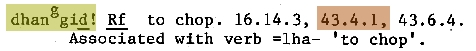
\includegraphics[width=\textwidth]{\imgpath/Thieberger2-img2.jpg}
\label{thi:fig:fig1a}
}
\subfigure[Excerpt from \citet{Heath1980}]{
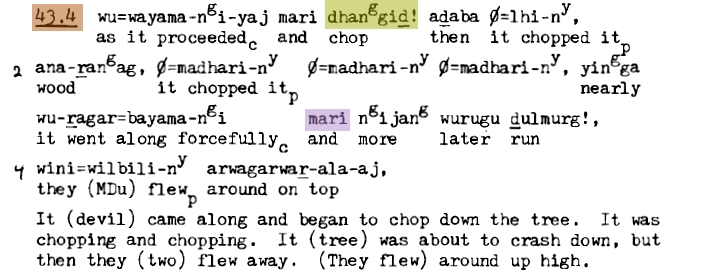
\includegraphics[width=\textwidth]{\imgpath/Thieberger2-img3.jpg}
\label{thi:fig:fig1b}
} 
\subfigure[Excerpt from \citet{Heath1984}]{
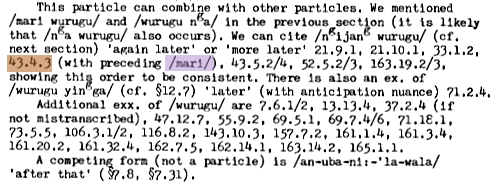
\includegraphics[width=\textwidth]{\imgpath/Thieberger2-img4.jpg}
\label{thi:fig:fig1c}
} 
\caption{Examples of linking between Heath's volumes} 
\label{thi:fig:fig1}
\end{figure}

The reader should bear in mind that we have carefully extracted these relevant sections from three separate books; in order to follow Heath's description to this level of detail requires manipulating and navigating three discrete physical objects.

Heath was very clear in his intention in following this practice. He emphasised in the introduction to the grammar volume that he was concerned with documentation: 

\begin{quote}
 These textual citations serve several purposes. When attached to a fully cited Nunggubuyu ex[ample], they have basically a documentary value -- the reader is assured that the ex[ample] is from a real text, and a reader wanting to know more or having doubts about the analysis can find it and analyse it.  [{\dots}] In this way, we take maximal advantage of the published texts (especially NMET*) achieving a far higher level of documentation than is observable in other reference grammars.'' \citep[4]{Heath1984} (*NMET = Heath 1980)
\end{quote}

And with accountability (see also Maxwell, this volume):

\begin{quote} 
 My concern with documentation reflects my own sad experiences as a reader of other linguists' grammars, which have almost never provided me with the information I wanted to undertake my own (re-) analysis of the language in question. It also reflects my experience that most published grammars are based on material obtained in unreliable direct-elicitation (sentence-translation) sessions [{\dots}] I have no confidence whatever in such data, since my own early `data' of this type often turn out to be seriously wrong. \citep[5]{Heath1984}
\end{quote}

However, these aims came at a price in terms of useability. In the course of otherwise extremely positive comments, two reviewers drew attention to the complexity of the work:
\begin{quote}
 ``Unfortunately, F[unctional] G[rammar of] N[unggubuyu] is a very demanding work, both because of the inherent complexity of the language and because it requires the reader to make constant reference to the text volume.'' \citep[310]{Blake1985} 
\end{quote}

\begin{quote}
 ``the work is particularly difficult to read. H[eath] makes no pedagogical concessions to the reader. One must look up the attestations for every major grammatical point in another volume.'' \citep[654-655]{Haiman1986}
\end{quote}

The linking structure which Heath included as an essential element of his description of Nunggubuyu lends itself naturally to treatment as hypertext links between documents,\footnote{The 
 fact that Heath's original recordings from his fieldwork are archived accessibly at the Australian Institute of Aboriginal and Torres Strait Islander Studies is an additional factor in our decision to work with this description.
} 
and we suggest it can serve as a first model for the structure of grammatical description in this format. For this model to be usable with new language data, it is necessary to establish encodings which, on the one hand, can be easily transformed into presentation formats while, on the other hand, still being formats with which linguists can work.

\section{Encoding issues}\label{thie:sec:3}
\subsection{Orthography }\label{thie:sec:3-1}
Heath uses a practical orthography to represent Nunngubuyu. This includes digraphs \graphem{n\textsuperscript{y}} and \graphem{n\textsuperscript{g}} to represent palatal and velar nasals respectively, and underlining of \graphem{t,d,r} to represent retroflex consonants. This system differs slightly from the system favoured by the speaker community today.
Our aim is to preserve Heath's orthography and to use transformations
to produce output in the current orthography where this is required.
As Unicode does not treat underlined characters as unique glyphs, in
basic formats we treat retroflex consonants as sequences of an
underscore followed by the relevant character (which can be rendered
by U+0331, the 'combining macron below' when necessary).


\subsection{Interlinear Glossed Text (IGT)}\label{thie:sec:3-2}
IGT is a common and extremely useful representation of bilingual text, capturing the complexity of the structural elements in the focus language in a morphemic level of annotation and providing a sentence-by-sentence translation at the free gloss level. Despite its ubiquity in linguistic description and despite theoretical modelling of various kinds\footnote{including 
  \citet{BowEtAl2003}, 
  \citet{HughesEtAl2003},
  \citet{HellmuthEtAl2006},
  \citet{Schmidt2003},
  \citet{Jacobson2006}, 
  \citet{JacobsonEtAl2001}, and \citet{PalmerEtAl2007}.
}
there is still no standard format for IGT that we could adopt in this model of linked Nunggubuyu data. The most common tool for creating IGT is probably \textit{Toolbox} with the benefit of lookup functions that allow parts of a corpus to be linked to the lexicon, to concordances and to specific wordlists \citep[see e.g.,][]{Hirzel2001}. The successor to Toolbox, \textit{FieldWorks,} addresses issues of interlinking by use of an underlying database, with the possibility of export to XML which may capture the relationships, but, if so, it is not clear to us what the schema is that allows these relationships to be encoded in the text.

Typecraft\footnote{\url{http://typecraft.org}} 
is a system for presenting interlinear text online served from an underlying database and uses Mediawiki, as does  Nordhoff's 2008 GALOES\footnote{ \url{http://www.galoes.org/}} which constructs an interlinked grammatical description. While these are ways of representing IGT using XML, there is no standard schema that provides a means for creating and linking between instances of IGT. Thus, for example, the online database of interlinear text (ODIN\footnote{ \url{http://odin.linguistlist.org/}}) which searches the web for likely examples of IGT, has to infer what IGT may look like from the alignment of text over several lines. Inevitably, such an inferencing approach results in many false positives and the data needs to be manually screened before it can be deemed to be a true sample of IGT. With the adoption of a standard IGT format such examples could be identified by web services and permit the retrieval of all and only IGT examples. 

In the Heath example under discussion, we opted to use EOPAS\footnote{ \url{http://www.eopas.org/}} \citep{SchroeterEtAl2006} both because it is a proposed standard and because it is built to work with primary media (as discussed in the next section). EOPAS is designed to take files in formats commonly created in the course of analysis, for example Toolbox IGT with timecodes linking the text back to the primary media, which it then transcodes to its schema. It also transcodes the media to formats playable using HTML 5 and highlights the textual chunks as their timecode is reached. As each utterance in EOPAS is citable to the level of the morpheme we are able to link from external objects, in this case the grammar and dictionary, to and from the morphemic level of an EOPAS file, as can be seen in the online example.\footnote{\url{http://users.monash.edu.au/~smusgrav/Nunggubuyu/17.HTML}}

\subsection{Media}
In what could be considered an additional or fourth member of the `Boasian trilogy' the audio or video recordings resulting from most fieldwork provide the basis for transcriptions and subsequent analysis. Maintaining the connection between the media and the derived or secondary materials (using Himmelmann's 2012 terms), \nocite{Himmelmann2012} as discussed earlier for the other outputs of language documentation, is now easily achieved and is slowly being taken up by linguists. A primary requirement of the citation of such media is that it have persistent identification which is provided by lodging the data in a suitable repository. Some repositories allow the media to be played directly from the archival location, while others allow for derived versions of archival material to be housed in accessible locations. EOPAS, discussed above, displays synchronised IGT and media and can either play from existing media files or from files uploaded to the EOPAS server. We included the media for a single text in our current project and encoded the IGT in a format suitable to allow for an EOPAS representation.

\subsection{Lexicon}\label{thie:sec:3-4}
There are a number of encoding formats for lexica which have been proposed or are in use \citep[for a slightly dated summary, see][]{Maxwell2008}. We have considered three\footnote{We 
 preferred these three options over the TEI dictionary format (\url{http://www.tei-c.org/release/doc/tei-p5-doc/en/HTML/DI.HTML}) mainly due to their being more targeted on small bilingual dictionaries.
} of these in developing this project: the Lexical Markup Framework (LMF\footnote{ \url{http://www.lexicalmarkupframework.org/}}), the Open Language Interchange Format (OLIF\footnote{ \url{http://www.olif.net/}}) and the Lexical Interchange Format (LIFT\footnote{ \url{http://code.google.com/p/lift-standard/}}).

Both LMF and OLIF have emerged from the environment of natural language processing and computational linguistics, and as a result both have rather Eurocentric models of the categories relevant to lexical data. In the case of LMF, this is perhaps less problematic as the data categories are kept separate from the specification of the format \citep[16]{Maxwell2008}. However, neither of these formats intuitively maps to the models of the lexicon used by descriptive linguists. Therefore we have preferred to use the Lexicon Interchange Format (LIFT) developed by SIL as our encoding scheme for the lexicon \citep{Hosken2006}. This format is intended to provide a well-structured XMLversion of the type of lexicon commonly used by linguists working with the Toolbox software and its successor FLEX. These software tools are popular with descriptive linguists, and using an encoding which is close to their file formats has obvious advantages.\footnote{Heath's 
 work on Nunngubuyu predates the availability of Shoebox (the precursor of Toolbox). The Nunngubuyu dictionary does exist in electronic form, as a Filemaker database.
} 
LIFT is also explicitly an \textit{interchange} format and we expect that scripts will become available shortly to move lexical data between this format and other popular and well-supported formats, including LMF and OLIF.

Figure \ref{thi:fig:fig2} shows an example of a LIFT encoded lexicon entry. Note that the  \tag{example} elements in this entry consist only of a reference to a source. This follows exactly Heath's practice in his dictionary. For our purposes, what is important is that the source information stored as an attribute in that element can be accessed and parsed to create a hyperlink to the relevant section of text when the lexicon entry is transformed into an HTML page. The `source' attribute is given here as a reference that can later be converted into a persistent identifier or URI, depending on the context in which the documents are delivered.

\begin{figure}
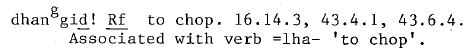
\includegraphics[width=\textwidth]{\imgpath/Thieberger2-img5.png}

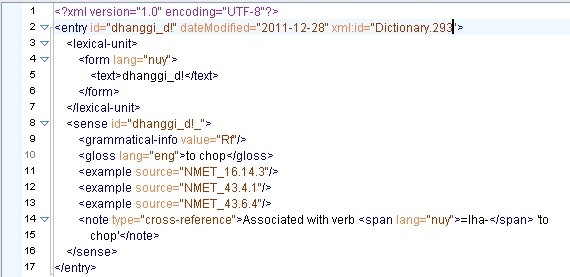
\includegraphics[width=\textwidth]{\imgpath/Thieberger2-img6.jpg}
\caption{Entry from \citet{Heath1982} with corresponding LIFT record} %
%This seems to be slightly inconsistent with the description and encoding below for the grammar: one would expect attributes like `source=``Text.16.14.3''~'.
%But indeed, given the possibility of interlinking arbitrary online resources, the ``source'' (and ``ref'') attributes should probably contain a more complete reference, ideally a PID (combined with an internal indication of the paragraph / entry / line etc.).
%
%NT {}-- I think these are fine and can be rendered as required by the next iteration of the program, as URIs or whatever. I've added a note to that effect above
\label{thi:fig:fig2}
\end{figure}

This entry also includes an identifier attribute in the  \tag{entry} element which is not a part of the LIFT format (\texttt{@xml:id}). This attribute is used for tracking references between the dictionary and other parts of the description; fuller discussion is presented in the following section. The numeric code is derived from the existing electronic version of the dictionary.

\subsection{Grammar}
We have already mentioned in section~1 that descriptive grammars have a more or less standard format. However, this format is a normative set of expectations about the order and means of presentation (see papers in \citet{EvansEtAl2006}, and in \citet{PayneEtAl2006}), rather than an accepted template, and it is therefore not surprising that no encoding for this document type exists. There are various kinds of encodings for grammars, including computationally tractable grammars (see also \citet[376]{Thieberger2009} on steps toward embedding a grammar in data), but we are here concerned with a marked-up textual encoding that permits interlinking. Our strategy in this example is to base our encoding on the Text Encoding Initiative Guidelines (TEI Consortium, no date) with additional elements as required.

The overall structure of the project requires that references from within the grammar to other parts of the description should be consistent in form and easily transformed to URLs which will point to relevant pages for online presentation. Heath's text already includes references to examples in the volume of texts and internal cross-references to other sections of the grammar. Although Heath does not include explicit links between the grammar and the dictionary, we wish to allow for such links in our version of the description. Such links are certainly implicit where Heath discusses specific lexical items within the grammar, and making the linking explicit is of great value as the language has considerable morphophonemic complexity which can make tracing lexical forms difficult. 

We encode all references with the TEI \tag{ref} element. This allows for the text representing the reference to appear in the document, thereby preserving the appearance of the original source. The location of the endpoint of a link is stored in the @target attribute of the  \tag{ref} element and takes the form of a pointer to the part of the description which is the target (Grammar, Dictionary or Text) followed by a numerical code. In the case of the grammar proper, the code matches the division shown in the table of contents and sub-heads; for example, chapter 7 sub-section 20 is coded as  \tag{ref target="Grammar.7.20"}. References to texts follow Heath's practice and specify the text identifier, a section number and a line number; for example a reference to line 2 of the third section of text 157 is encoded:  \tag{ref target="Text.157.3.2"}. The line numbering is an artefact of the original document; we have not yet encoded a large enough sample of the text collection to know whether this information will actually be useable in the web presentation or whether the interlinear presentation described in Section \ref{thie:sec:3-2} will rewrap texts in a way which makes this level of detail redundant. Retaining information from the source is of course best practice in this situation. References to the dictionary are to numerical codes which are an artefact of the existing electronic version of the material (FileMakerPro database); for example a reference to the lexical item \textit{i:-jung} is encoded:  \tag{ref target="Dictionary.4720"}. 

In all cases, the target material has to be coded with an identifier which exactly matches the originating pointer. This is done with an \texttt{@xml:id} attribute included in the relevant element of the different types of material. This coding has already been illustrated with the lexical entry example in Figure \ref{thi:fig:fig2}; similar attributes are attached to the  \tag{div} element which contains each section of the grammar and to the element  \tag{phrase} which holds each section of each text (and this can focus down to the level of  \tag{morpheme}). Figure \ref{thi:fig:fig3} is a section of grammar text with all three types of reference illustrated: line 57 includes a reference to the dictionary (created in our encoding), line 61 includes internal references to other parts of the grammar, and lines 78ff include references to text examples. 

\begin{sidewaysfigure} 
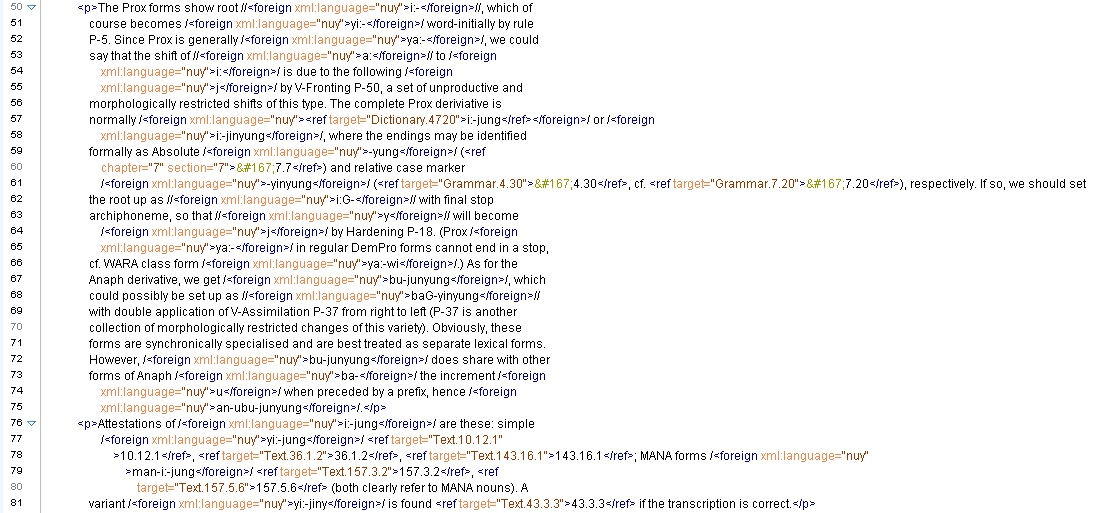
\includegraphics[width=\textwidth]{\imgpath/Thieberger2-img7.jpg}
\caption{Section of encoded grammar (from Heath 1984, section 7.25)}
\label{thi:fig:fig3}
\end{sidewaysfigure}


One additional type of reference occurs in the grammar, that is, citations of other works. The online presentation has a bibliography page, and citations are therefore encoded as pointers to items on that page. For example, a reference to Hore (1978) [1979]\footnote{Heath 
 1984 lists this work as Hore 1979; however the date of issue for volume 17 of \textit{Oceanic Linguistics} is 1978. Our internal reference retains Heath's error, but the Bibliography page includes a correction and clarification.
} \nocite{Hore1978}
is encoded as  \tag{ref target=``Bibliography.Hore.1979''}.

Figure \ref{thi:fig:fig3} also shows that we make extensive use of the TEI  \tag{foreign} element to encode words and phrases which are not English. In fact, all the examples of this element in figure \ref{thi:fig:fig3} enclose Nunggubuyu material, but in other places Heath includes cognate forms from other languages and the use of the \texttt{@xml:language} attribute is not redundant. 
 
\section{Further Development}
A small segment of the description of Nunggubuyu is available online at \url{http://users.monash.edu.au/~smusgrav/Nunggubuyu}. The XMLsource of these pages was hand-coded and HTML was then generated using search-and-replace in a text editor. Obviously, these procedures are time-consuming and, having established reasonably stable principles for encoding the material, our next priority is to automate the process as much as possible.

A first step in this endeavour will be to attempt to produce electronic versions of the original texts using optical character recognition software (OCR). As discussed in Section \ref{thie:sec:3-1}, Heath's texts use an idiosyncratic orthography with superscript characters which are important. The original text also uses subscript characters in gloss lines to indicate various grammatical properties. All of these characters will need to be captured by OCR if the process is to be useful. Even if OCR is successful at that level, it will still be necessary to use scripts to insert some appropriate encoding of the non-standard characters. It seems quite likely that the post-editing which will be needed to make an OCR version of the material useable may be so extensive as to render the whole process too slow. The alternative then would be to have the source materials retyped directly to our preferred encodings%
%See Michael Cysouw's dictionary project: he sends all his scanned material to (south)east Asia for re{}-typing and is content with both prices and results.
%
%Right, and we would potentially do that too, but it is not necessary to state it here.
; this would also be time-consuming (and expensive), but may be a more efficient alternative. If OCR turns out to be a viable means of generating a complete electronic version of the material, we would still need to develop scripts to add encoding to the basic text. This is still not a particularly attractive option as such scripts will be specific to the source with which we are working. If in the future we wished to import another pre-existing description to our format, we would almost certainly need to at least considerably modify the scripts used to add mark-up.

Various issues concerning the internal linking of the materials will arise when we are able to work with the entire description. As noted in Section \ref{thie:sec:3-4}, we believe that it will be useful to include  links explicitly which Heath left as implicit%
%Another case are the constant cross{}-references to RULES (such as P{}-5, P{}-50 etc. in Fig.~3), which should also correspond to  \tag{ref} elements.
, such as those pointing at rules (such as P-5, P-50 etc. in Figure \ref{thi:fig:fig3}) or between lexical forms in the grammar and corresponding dictionary entries and those between dictionary entries which are cross-referenced. Three questions will have to be addressed in generating such links. First, to what extent is it useful to make the implicit structure explicit? There are cases where doing so is clearly advantageous; in the following paragraph we discuss an instance where we have included a reverse link (from text to grammar) to complement the link Heath made between grammar and textual instance. But we can imagine that in some cases fully explicit linking might be counterproductive: will the user always want to have access to every textual instance of a common morpheme? It will be desirable to allow the possibility that a user can search for every instance, but listing every one with an explicit link would probably be unnecessary (See Good's (this volume, section 8.1) distinction between examples and exemplars{}---the latter being carefully selected to illustrate a point, while the former are more or less the harvested results of a search). %
%See Jeff Goods distinction between examples and exemplars {}-- the latter being selected by hand.
Second, how can this process be done automatically? This is only a problem for dictionary entries as references to texts and to sections of the grammar will always be in a form (numerical code) which can be parsed automatically. For the dictionary, however, we believe that it will be necessary to create a look-up table against which the texts and grammar can be compared to identify forms which should be linked to dictionary entries. The third question to be considered is whether the resulting structure should be implemented as simple hypertext links, or whether it will be more stable and efficient to use a link table (that is, a simple database) to store the links. Doing so will mean using some scripting language to actually implement the links, and this is not desirable; in principle, we would prefer to keep the whole implementation in HTML only. However, there are additional considerations, to which we now turn, which suggest that such an HTML only implementation will not be practical.

Even in the very small sample which we have produced so far, we have encountered a problem in realising the complexity of the links which allow the user to move from one part of the description to another. In the text sample online, we have linked some forms to their dictionary entries; this has been implemented at the morphemic level of the text. But there is one case (\textit{da:n} in line 1 of the text) where we have also implemented a link from this morpheme to a section of the grammar. This is a link which is only implied by Heath: the grammar refers to the text as a relevant example, but there is no annotation in the text to indicate the relevance of the grammar section. There are thus two targets linked from a single source morpheme at this point. We have dealt with this by instantiating the link to the dictionary on the morphemic analysis line and the link to the grammar on the text line, and this is an adequate solution in this case. However, we are aware that there will certainly be cases where a single form in a text will need to be linked to more than two targets. For example, a motion verb form might be linked to a description of the class of verbs to which it belongs, to an analysis of the morphophonemic changes which the form undergoes as well as to a discussion of how directionality is treated in the language. With a link to the dictionary as well, this will require four links to be instantiated from only two source forms, which is not possible using HTML only. We suspect that we will want to use a technique such as menus which pop-up when the cursor is over a form in order to handle this sort of complexity. We also suspect that, when the full complex structure of links is created, the actual appearance of texts on the screen will be problematic. Every form, or almost every form, will be the source of a link. 
If these links are simple HTML links, then (almost) every form will
be a link, making it difficult to visually distinguish links from
non-links in the text. This is  problem that we expect to be able to
deal with using style-sheets in the delivery version. If we need to use some programming resources to handle multiple links from a single source, then it will probably be worth also using such resources to implement links to the dictionary with keystrokes. For example, selecting a form on the morphemic tier and using the keys \texttt{Alt+D} would take the user to the relevant dictionary entry in every case. We also anticipate that there will be problems to solve for links to grammar sections which discuss constructions rather than individual forms. It is not immediately clear whether the source of such links should be individual words or morphemes, or the entire span of text which is relevant. 

The various questions just raised will become relevant when we have all of the description encoded and potentially available as hypertext. At that point, we expect to have to make decisions about how to deal with the problems and this will most likely mean making a decision about a programming or scripting language to use to develop the online environment which we want. 

A further and critical matter to be confronted in the creation of any data is the longevity of the material created. As stated earlier, one motivation for encoding a grammatical description is explicitly to allow the rich set of links implicit in a grammar to be stated and stored as text, a preferred archival format. Persistence of the primary media and any secondary analysis would, as a matter of course, be provided by an appropriate repository and the links between objects described here would resolve to these archival forms or derived versions (as HTML, or streaming media for example) in suitable locations. Although we have introduced the possibility that delivery in a browser will require resources beyond those offered by (current versions of) HTML, our approach ensures that the linking structure is explicitly encoded in archival data sources. Optimal presentation may depend on particular implementations, but presentation is independent of the basic data. We note that in the case where the data is not derived from printed material, this means that a rendering as a printed object will also be easily achieved.

\section{Designing Electronic Grammaticography}
Electronic grammaticography is the topic of all chapters in the present volume, and also of \citet{Good2004}, \citet{Nordhoff2008}, and \citet{BenderEtAl2004}. Our project is offered as an example both of retrofitting an existing grammatical description and of setting out what requirements more elaborated grammar-template projects could include. We have described here the preliminary stages of a project which aims to make a classic grammatical description available as an electronic resource. We have discussed a number of problems which arise in transferring such material from its original form as printed text to a new format which makes new and richer possibilities available, and the reader might be tempted to ask whether there is any point to grappling with such problems; might it not be simpler to work with newly-produced materials which are already available in electronic formats? Obviously, we believe that the effort is worthwhile, and we would like to close by offering some of our reasons for this view and showing how they relate to basic issues in the development of electronic grammaticography.

First, most of the problems we have discussed in Section \ref{thie:sec:3} are about choosing suitable formats and encodings for source material. Most of these problems would still need to be faced in working with recent materials. Many linguists work with texts and lexicon in Toolbox, but this practice is not universal, and even those who do structure their files differently. Even for material originating in Toolbox, decisions would need to be made about a common encoding to be used as an interchange on the way to online presentation, and such an encoding would also have to be used for materials from other source software. Although the practical problems of transferring material from one format to another would be simpler for description born digital, the conceptual issues would be the same. And for actual grammatical description, the range of formats used by different scholars would be considerable; again the conceptual issues are the same as those we have discussed. (If we are able to present grammatical description online in a useful and attractive way, we would hope that other scholars might then adopt our encoding practices, but we are not aiming to impose a standard on our colleagues, only to find a pragmatic solution.)

Second, we believe that it is important to be able to handle grammatical description which already exists as legacy materials. The advantages which we see for the mode of presentation discussed in Section \ref{thie:sec:1} are considerable. Assuming that we can achieve the aims which we have set out here, we believe that it will be very desirable to make as broad a range of grammatical materials as possible available in this way. 

Third, and following from this previous point, we believe that the design of electronic grammaticography should incorporate the best practice of traditional grammaticography and then extend it. Heath's work is an ideal starting point for this endeavour. As we discussed, Heath had a carefully considered view of how the parts of his description should interact for the user. The format which was available to him made this very difficult in practice but we can now attempt to implement that interactivity in a more congenial format. Even replicating what Heath included in his work means addressing fundamental questions about how electronic grammaticography can work. Going beyond Heath and making the web of interconnections more complete and more explicit poses additional problems. We suggest that adequate solutions to these problems will provide a sound basis for one version of electronic grammaticography. 


\documentclass{article}
\usepackage[utf8]{inputenc} % please use UTF8 encoding
\usepackage[T1]{fontenc} 
\usepackage{gb4e}

\begin{document} 
% This file was converted to LaTeX by Writer2LaTeX ver. 1.0.2
% see http://writer2latex.sourceforge.net for more info
\documentclass[letterpaper]{article}
\usepackage[ascii]{inputenc}
\usepackage[T3,T1]{fontenc}
\usepackage[english]{babel}
\usepackage[noenc]{tipa}
\usepackage{tipx}
\usepackage{amsmath}
\usepackage{amssymb,amsfonts,textcomp}
\usepackage[top=0.4917in,bottom=0.7874in,left=0.9839in,right=0.9839in,includehead,head=0.4925in,headsep=0.4528in,nofoot]{geometry}
\usepackage{array} 
\usepackage{hhline}
\usepackage{hyperref}
\hypersetup{colorlinks=true, linkcolor=blue, citecolor=blue, filecolor=blue, urlcolor=blue}
\usepackage{graphicx}
\begin{document}
\clearpage\setcounter{page}{1}\pagestyle{Standard}

\end{document}


\end{document}



\glossSTDmode
\setcounter{exx}{0}\setcounter{footnote}{0}
\renewcommand{\imgpath}{./Baraby}
\renewcommand{\thischapteruuheader}{\uhheader{78-101}{4531}}
 
\renewcommand\chapname{Grammars for speakers}	
\renewcommand\longchapname{Reference grammars for speakers of minority languages}
\renewcommand\shortauthor{Anne-Marie Baraby}
\renewcommand\longauthor{Anne-Marie Baraby\\ Université du Québec à Montréal}
\chapter*{\longchapname}
\chapterauthor{\longauthor}
\mytoc{}
 
\begin{abstract}  
Most of the work done in grammaticography focuses on the writing of grammars for an audience of linguists, and more specifically, typologists. In this paper, we present a grammaticographic model designed mainly to take into account the needs of minority language speakers, because they play a central role in the preservation of their language. However, since in minority language situations it is not possible to generate as many grammars as there are different potential end users, we propose a multilevel grammar, based on our experience as grammarian of Innu, a First Nation language spoken in Quebec (Canada). In this type of grammatical description, the first (main) level is addressed to non-specialist users, the speakers of the language being described, whereas grammatical material aimed at other users (such as linguists) is presented in secondary levels and is limited to core information. Our grammaticographic model was initially conceived for paper (printed) grammars, but we believe that electronic publication offers interesting solutions for multilevel grammars, while paper (printed) grammatical descriptions have greater limitations.
\end{abstract}

\section{Introduction}
Grammaticography as a new branch of linguistics was developed almost at the same time as documentary linguistics \citep{GippertEtAlEd2006}.\footnote{Thanks 
 to Sebastian Nordhoff and to an anonymous reviewer for their comments on an earlier version of this paper, and thanks to Robert Papen not only for his comments, but especially for the revision of the English text.
}  The development of these new domains of linguistics in the recent past is not a coincidence. In fact, there is a link between both domains, since the development of a grammar is theoretically part of a documentation program for endangered languages. Furthermore, these fields of research were proposed as solutions, among others, in preventing language extinction. But, without denying merit to those who drew up the basics of grammaticography, we believe it maintains an important weakness: most of the work done in grammaticography, i.e. the business of writing grammars, aims the grammatical descriptions primarily at linguists, usually ignoring the minority language speakers, who have their own specific needs. However, we believe that the speakers of an endangered language play a central role in documenting their language, even though they are not specialized in linguistics. Therefore, in our PhD thesis  \citep{Baraby2011a}, we propose a model of grammaticography which takes into account speakers' needs. More precisely, from our experience as a grammarian of Innu, an indigenous language spoken in northern Quebec, we have developed a set of principles which may help in constructing a model of a reference grammar intended particularly for Innu speakers.

Developing a reference grammar for a minority language, often under-documented, usually unwritten, and probably endangered, is quite different from writing a grammar for languages of wider communication such as the main Indo-European languages. In the latter case, it is possible to generate as many grammars as there are different theoretical approaches, different end users, and different objectives. This situation is highly unlikely for most minority languages, where it is generally impossible to develop such a multiplicity of different grammars. In short, writing a grammar for a minority language raises the following question: is it possible to develop a reference grammar aimed at both types of audiences, linguists and non-specialized users?

Actually, writing grammars for non-specialized speakers brings its own challenging issues, which are different, in many regards, from grammaticography conceived for linguists. In the following sections, we will deal mostly with the question of the end users of a particular grammar and the solutions we propose in achieving the task of documenting a language mainly for the speakers of that language, but also for any other interested public, such as linguists who want to learn something about the inner workings of the language. Among the means we propose for such a grammar, based on our experience in the Innu language grammar project, is a multilevel grammar, which we believe can be achieved both in printed and electronic versions. Would an electronic grammar be a better medium for the model of grammar we are proposing? At first glance, it may seem so. However, we do not see the two media types as being opposed, but as complementary options. In our view, developing a grammar on Internet may pose specific challenges, but it also shares problems with writing a grammar for a printed book version.

\section{The problem} Developing a grammaticography for users without specialized training in linguistics raises a number of issues, including the selection of the eventual end users and specific objectives.\footnote{In
 our thesis, we also discuss the following issues: possible types of grammar, language register, compari\-son with other languages (related or not), language variation and linguistic norms, description of an oral and/or written language, use of the orthography (if there is one), use of parts of speech, presentation of examples.
}
Among others, these issues concern different choices regarding the theoretical approach, the language used in writing the grammar itself, including the grammatical terminology and metalanguage, and the depth of the grammatical description envisaged. Furthermore, there are questions referring to the content itself, for instance which phenomena to describe, the scope of the description, the organization of the content, etc. And finally, the issue of the type of grammar planned is also often raised as to whether it is to be a pedagogical grammar or a reference grammar. 
Since we believe that the choice of who the eventual end users are to be determines all the other choices made by the grammarian, the following discussion mainly concentrates on this particular issue. 

In our grammatical model, we place the speakers of the language being described in the foreground. But making this basic choice is not as easy as it appears because, as previously stated, in the case of minority languages, the possibility of being able to produce more than one reference grammar is very low to non-existent. Therefore, even if we choose to produce a grammar mainly for speakers who are not specialized in linguistics, we are aware that it is also important to document the language for other users, including linguists, but only as secondary end users. However, such a decision, which takes into account the needs of different types of users for the same product, raises a big problem: \textit{Is it possible to write a reference grammar for different users having different expectations}? This is a complex issue in a grammaticography mainly developed with the objective of documenting minority languages. Indeed, aiming at heterogeneous users could bring about dissatisfaction with the content of the grammar on the part of all users.

As a solution to this problem, we propose a multilevel grammar, where most of the content is addressed to a non-specialized audience, speakers of the described language (it constitutes the \textit{first} or \textit{main level}), but with some additional grammatical information (the \textit{secondary level}) aimed at specialists, such as linguists. More details about this type of reference grammar are given in Section~4.

Once the end users and the objectives of the reference grammar have been established, the grammarian must decide if the grammatical product is to be a printed book or an electronic document. Both media have advantages and inconveniences. In our thesis, we primarily discuss solutions to produce a good grammar for Innu speakers, with secondary attention paid to a specialized audience.\footnote{As
 specialised audience, we think of linguists working in typology, Algonquian linguistics, historical linguistics, anthropological linguistics, etc. } Here, we also intend to look at possibilities of electronic grammars, especially for the kind of multilevel grammar we are proposing for non-specialist end users. Is an electronic edition a better choice for such a grammar? It certainly offers good resources to produce the kind of multilevel grammar we are envisaging. However, since electronic tools are not available everywhere, and also because some users are not yet ready to use these tools, we believe that printed grammars will be maintained, according to users' needs or wishes. And even where electronic tools are available, both grammars can be seen as complementary ways to reach the main objective: documenting an under-described language, and giving speakers a tool to develop a good formal knowledge of their language.

\section{The Innu People and their language}
Before discussing our grammaticographic model further, below we give a short description of Innu\footnote{The
 Innu were previously called Montagnais by French speakers. They always called themselves Innu (`human being', now `Amerindian' and `Innu First Nation') and it is this term that is now officially used not only by the Innu organizations, but also by federal (Canadian) and provincial governments, and in the media.
} 
communities and their language, because we think their linguistic situation may be comparable to many other minority linguistic groups, and above all, because it is their linguistic situation that convinced us to work on a reference grammar of their language. Even if we are well aware that all sociolinguistic situations are not identical, we believe that the grammaticographic principles and solutions we are proposing may be useful elsewhere. 

\subsection{The linguistic, geographic, and demographic situation of the Innu communities} 
Innu is part of the Algonquian language family and is spoken in Quebec and Labrador. It is closely related to Eastern Cree, also spoken in Quebec, and to Naskapi, spoken in Labrador. The Innu live in ten isolated villages spread out over the immense northern territory of Quebec and Labrador, Canada. Some of these communities still cannot be reached by road. Around 10,000 people use Innu as a first and every-day language. The rate of retention of the language varies from one community to another: extinct in one, spoken by one third of the population in another, majority language of nearly 75~\% to 95~\% of the population elsewhere. The Innu language therefore is still very vigorous in a majority of Innu communities, where it is the first language learned by children and is used at home and in the community at large. Except for two communities (Mashteuiatsh and Essipit), Innu is also used in religious ceremonies, local administration, community radio, and, with the intervention of interpreters, in health, social and legal services.

Nevertheless, pressures from the dominant language are very strong, since virtually all Innu are bilingual today, with French as their second language in most Quebec communities, and English in the Labrador community (and partly in Pakuashipu, Quebec). If Innu is not considered endangered enough to disappear in the short term, its survival is not guaranteed in the long term, because of the relatively low number of speakers. 

The Innu language constitutes a continuum of dialects, geographically spread out from the most western one, Mashteuiatsh (Lac Saint-Jean), the ``central'' dialects, with Pessamit, Uashat-Maliotenam on the upper north shore of the Saint Lawrence and Matimekush (Schefferville, Northern Quebec), and Mamit (on the lower north shore of the Saint Lawrence), as well as Ekuantshit, Natashquan, Unamen-Shipu, Pakua-shipu; the dialect of Sheshatshiu (Labrador) is somewhere between the central and Mamit dialects. These dialects are quite different, morphologically or phonologically speaking, but speakers of different dialects still readily understand each other. 

Much as for most Amerindian languages, Innu was until lately an oral tradition language, but a standardized writing system has been developed, except for Mashteuiatsh (Lac Saint-Jean, Quebec).\footnote{Because
 the Mashteuiatsh dialect is different from other dialects (it is more conservative) and it is learned by children as a second language, the community did not adopt the standardized orthography. We are now working with the community to develop their standard writing.
}
However, this standard orthography is not necessarily mastered by all speakers, who more often turn to French (or English) for their written communications. In fact, oral and writing habits are diglossic: Innu for oral communication within the community, French elsewhere.\footnote{To
 know more about the development of a standard orthography and the role of writing in Innu communities, see \citet{Baraby2000,Baraby2002,Baraby2011b}.
}

\subsection{The Innu language in schools}
Locally, Band councils run all Innu schools, from kindergarten to high school. More and more Innu teachers are teaching in these schools, however most of these certified teachers are not involved in Innu language teaching: they teach the various subject matters determined by the regular provincial programs, using French or English in the classroom. In fact, these teachers prefer to teach these subjects since they are properly supported with well designed curricula and pedagogical material.

If Innu is indeed part of the school curriculum, usually taught once or twice a week (1 or 2 hours/week), the working languages of the school, including the languages in which academic subjects are taught, are French in Quebec and English in Labrador. Also, except for help from the \textit{Institut }\textit{Tshakapesh} (see below), Innu language teachers, all competent speakers, but without adequate training in linguistics, Innu grammar, or even language teaching pedagogy, are often left quite isolated in their specific teaching tasks. In fact, teaching Innu is not perceived as being as attractive as teaching regular subject matters. Nevertheless, in spite of all these difficulties, the Innu language teachers are highly motivated in transmitting their language, and in learning more about it.
 
Fortunately, a university program for the teaching of Innu has recently been developed. Also, tailor-made courses in linguistics for Innu teachers are now offered two or three times a year,\footnote{The
 Université du Québec à Chicoutimi is providing two undergraduate certificates (10 courses each) specially designed for First Nations~: \textit{Technolinguistique autochtone}, \textit{Transmission d'une langue autochtone}.
}
as well as workshops on language teaching. The \textit{Institut Tshakapesh}\footnote{\url{http://www.icem.ca/icem/}} (a cultural and educational institute for the Innu people, based in Sept-Îles, Quebec) has taken leadership to promote Innu language preservation and development. The institute supports Innu teachers in different ways, including the organization of meetings, workshops and courses, funding the production of curricula, pedagogical materials, reference materials, hiring specialists in linguistics or in language pedagogy, etc.
Except for the two communities mentioned above,\footnote{In
 these two communities (Mashteuiatsh and Essipit), Innu is taught as a second language.
}
where the language is not spoken by children, Innu is taught as a first language to students who are already fluent in it. The students are expected to improve their oral skills and acquire literacy in Innu. Since the traditional way of life has changed a lot, language transmission has also changed. Parts of traditional vocabulary are being lost, and the language of the youth now includes more and more loanwords, systematic code switching and code mixing (with French and more rarely English). At this point in time, we do not know if pressures from the linguistic environment have already altered certain grammatical structures of Innu, but it is quite possible. Thus, Innu language courses in the school curriculum have an important role to play in preventing language erosion or loss, as do the families and communities themselves. 

\subsection{Documentation of Innu} 
Innu is probably one of the most documented languages of all of the native languages of Canada, but except for dictionaries published since the 70s, the majority of linguistic descriptions was intended for linguists and published in academic journals.
At present, there exists no comprehensive reference grammar for Innu, but we are now working on such a grammar, specifically aimed at Innu speakers (Baraby \& Drapeau, forthcoming). A conjugational guide  \citep{Baraby2004} is however available, and some electronic learning material is also presently being developed.\footnote{Marie-Odile
 Junker, a linguist from Carleton University (Ottawa) and specialist of Eastern Cree, has developed electronic material for the Cree in Quebec (url{http://www.eastcree.org/}{textstyleInternetlink{www.eastcree.org}}), and she is now collaborating with the Institut Tshakapesh to elaborate similar kinds of material for Innu, mostly for pedagogical use.
}

The completion of a reference grammar will answer a pressing request which comes from the Innu themselves, particularly from Innu language teachers. This reference work is necessary to help Innu speakers develop metalinguistic knowledge about their language. As well, it will be a good tool in supporting the development of pedagogical material and literacy.

In sum, producing a good Innu reference grammar, accessible to non-specialists, will give a good opportunity for linguists to transmit to non-specialized speakers the grammatical knowledge they have acquired over time. We believe it is an interesting way of assuring that specialized knowledge does not remain ensconced in academia, but returns to the most prominent actors in the maintenance of an endangered language, the speakers themselves.

We sometimes hear linguists say that minority languages speakers are not really interested in having a (written) grammar of their language. We understand that this is not a priority everywhere. However, the facts from the Innu language situation demonstrate quite the opposite: many Innu speakers are highly motivated to learn more about the grammar of their language, as long as they are given a reasonably easy access to it. 

\section[Grammaticography for minority language speakers]{A grammaticography intended for minority language speakers}
Our work on Innu grammar has raised a number of issues that led us to develop a grammaticographic model, conceived for non-specialists, i.e. the speakers of the language being described. Besides the targeted end users which we discuss in the next section (\ref{baraby:sec:4.1}), the main characteristics of this model are the following:
\begin{itemize}
\item The grammar is a \textit{reference grammar} rather than a \textit{pedagogical} grammar. This follows from the fact that the main objective is to document the language in a comprehensive way.\footnote{Pedagogical
 grammars are usually less comprehensive than reference grammars. The former usually have as objective the learning of a language as a foreign or second language, or the learning of writing rules based on grammatical structures. The organization (or progression) is also different in both types of grammar. Pedagogical grammars usually include exercises, while reference grammars do not. But the boundaries between both types are sometimes loose, since both types may have pedagogical purposes. In fact, the different types of grammatical descriptions are on a continuum, and a reference grammar for non-specialists is closer to pedagogical grammars than is a grammatical description specifically intended for linguists (see \citet[46-56]{GermainEtAl1995}, \citet[1-2]{Dirven1990}, \citet[210-236]{Baraby2011a} for further details).}
\item French is used to write the grammar as well as for the metalanguage and grammatical terminology, because the Innu are familiar with French from their schooling. Actually, they are more used to read in French than in Innu. Moreover, writing the grammar in a relatively well-known language such as French allows most users who are not speakers of Innu to read the grammar, including linguists or other interested users (see Section \ref{baraby:sec:4.3}). 
\item The writing style is rather formal, but with a simple and precise vocabulary.
\item Comparisons with French, English and other Algonquian languages are made, whenever they help users transfer their metalinguistic knowledge from one language to the other, for instance, from school knowledge (French grammar) to mother tongue. It is also interesting for Innu speakers to see the links between their language and other related languages such as Cree, Naskapi or other Algonquian languages.
\item Whenever possible, the grammatical terminology used to describe the language is the one used in traditional French grammars, because it is already familiar to most Innu speakers. However, terminology may also be innovative, in order to fill terminological gaps in traditional French grammar. Even if some typical Algonquian linguistic terminology is used, it is sometimes abandoned in light of the current knowledge of the language and in order to meet the particular needs of non-specialist users.\footnote{For
 pedagogical reasons, we may decide to abandon terms whose meanings are opaque to laymen. For instance, in Innu there is a mode with a counterfactual meaning, but the term `\textit{contrefactuel}' (counterfactual) is not well understood by Innu speakers. Also, other terms create confusion, for instance, \textit{subjonctif} (subjunctive) and \textit{subjectif} (subjective); in this case, we replace the latter with another term, \textit{percepti}\textit{f }(perceptive).
}
\item Innu is an oral tradition language, so the grammatical description focuses on this aspect, but it also takes into account standard orthography. For instance, examples are given in this orthography, instead of being transcribed in a phonetic alphabet. Phonetic transcriptions are minimally used, mostly in sections specifically addressed to lin\-guists.
\item Dialect variation is considered, but only to a certain point. The use of a standard\-ized orthography is a good solution in giving a more synthetic description that is accepted by all speakers.\footnote{The
 Innu orthography is not based on one particular dialect, but on principles such as the following : the Eastern (Mamit) dialect serves as a reference for grammatical spelling, while, when variations are more phonological, the Western dialect become the reference. In sum, speakers from all communities have had to compromise in arriving at an agreement on a common spelling system \citep{Baraby2000, Baraby2004}.} 
\item Even if the language spoken by elders is generally seen as the norm, i.e. ``good Innu language'', the speech patterns of all generations are considered in the grammatical description.
\item The general organization of the content is ``bottom up'', starting with the simpler notions, for instance the word before the sentence, the noun before the verb, etc. It goes from structures to functions or from functions to structures.
\item The theoretical approach is a ``traditional'' one, close to traditional French grammar, with additions to reflect particularities of Innu grammar; the latter being based on recent research by Lynn Drapeau, co-author of the grammar and specialist of Innu linguistics. In fact, this comes close to what   \citet{Dixon1997,Dixon2010} proposes in his \textit{Basic linguistic theory}: to describe languages in the perspective of language documentation.
\end{itemize}
Obviously, each of these characteristics could be discussed in more detail, but we will now focus on the issue of multiple end users for a grammatical description and the solution we propose to achieve this objective, a multilevel grammar.

\subsection{Targeted end users for a minority language reference grammar} \label{baraby:sec:4.1}
The status of the main readership of a grammar, i.e. the targeted end users, needs clarification, because each type of grammar user is in fact not homogeneous, some being laymen, other being linguists. Basically, we distinguish two main target groups: non-specialists, for instance language teachers (the primary group); and specialists, for instance linguists (the secondary group). Each of these two broad groups may be heterogeneous.

\subsubsection{Principal end user : language teachers} 
As  \citet[282]{Mithun2006} points out, non-specialized users are not all the same, depending on specific linguistic situations. Actually, a layman readership may include anyone interested in knowing more about the described language: speakers or non-speakers, teachers or students, advanced learners or beginners, first or second language learners, having basic, intermediate or advanced knowledge in the grammar or even none at all, literate in the language or not, etc. For Mithun, it is also important to think about the future needs of the members a language community: those who are not interested in or able to use the grammar at present could become users later on, for instance, after some training. 

For the grammar of Innu, we propose, as \textit{main}\textit{ end user}, those speakers who have some basics in grammar, if not in Innu grammar, at least in school grammar, that is in French grammar,\footnote{The
 complexity of written French grammar makes possible some transfer of grammatical knowledge from French to Innu; for instance, agreement rules or the complexity of verbal inflections. Since most Innu speakers learn French grammar in school, we want to take advantage of this fact. Of course, this advantage does not hold for those who have been schooled in English, as English grammar (at least morphologically speaking) is not as complex as French grammar.
}
for Quebec Innu speakers. More precisely, we choose Innu language teachers as targeted end users, for various reasons. First, because they are competent speakers of the language. Secondly, because they have had some grammatical basics in their language of schooling (French) and they also have a university degree in teaching, or they have had some training in pedagogy or in Innu grammar.\footnote{The
 older Innu teachers may not have a university degree, but they have taken a certain amount of tailor-made courses over the years. We hope that younger teachers will graduate in education, since the expectations from school administrators are getting higher for their teachers.
}
Finally and above all, because they are very motivated to learn more about the language they have to transmit to their students. Some of them, but not all, have had some basic training in Innu linguistics.\footnote{University
 Certificate programs in Amerindian language teaching and in ``technolinguistics'' (\textit{technolinguistique}), designed by the University of Québec at Chicoutimi, are now available. Innu teachers may enrol in these programs, and one or two courses are available every year. 
} 
As main end users, we would also add any other professionals involved in different areas related to the Innu language: language curriculum designers and developers of pedagogical material, translators, authors and writers.

In our grammaticographic model, we claim that minority languages require reference grammars rather than pedagogical grammars, in order for them to be well documented, and in a comprehensive way, and such a grammar is probably not for beginners, users without any skill in formal grammar. In other words, in the reference grammar model we propose, the level of difficulty is \textit{intermediate}, which means that main users are not specialists, such as linguists, but they have basic grammatical knowledge, if not in their first language, then in their second language. Of course, as mentioned above, this intermediate level may include other users than teachers such as language professionals, and, even advanced learners or any other person with basic grammatical competence.

\subsubsection{Secondary end users}
Linguists will also get something out of the kind of grammar we are proposing; either a starting point to their curiosity about the language, or an overall view of it, which could be completed with more specialized publications. For instance, Innu has been the subject of many academic publications in linguistics, but even specialists may find it useful to get all the information in a single place, instead of having to search for information scattered in different journals and books. Therefore, obtaining grammatical knowledge about a minority language in one single document, that is in a reference grammar for non-specialized speakers, is a good way of documenting a language, as much for linguists as for non-specialist speakers.

We now raise an important issue: Is the objective of documenting a language -- meaning that the grammar has to be as comprehensive or complete as possible -- compatible with the aim of producing a user-friendly grammatical description? On the one hand, comprehensiveness implies adding more complex information (usually addressed to linguists), such as information that may be necessary for better comprehension of the structure of the language and to the eventual development of linguistic typology. On the other hand, integrating this kind of material may be confusing to non-specialized users, especially if it is inserted in the main part of the description, that is, if it is included in the main grammatical text.

Considering the needs of different potential users in one single reference grammar may seem conflicting, especially with end users as different as non-specialized speakers and linguists. To achieve our objective of an accessible grammar, designed as much to document a language than to train and inform native speakers of it, we propose a document having more than one level (or layer) of reading, the main (first-level) text being user-friendly, with more specialized or complex information intended for linguists being presented at another level. In the next section, we will outline what we mean by a multilevel grammar. 

\subsection{A multilevel reference grammar}
 Is it possible to write a reference grammar for different users, with divergent expectations? For under-described languages, the choice is limited, since it would be utopian to expect different kinds of grammatical descriptions for each potential audience. As a solution to this issue, we propose our multilevel (or multilayered grammar), that is with each level being aimed at a specific audience.

\subsubsection{First level: main level} 
The first level, intended for specific users, speakers of the language but without specialized training in linguistics or in grammar, is the main level. This means that these end users have priority over all others, and that most of the grammatical content (explanations and descriptions) is found at this level. For that matter, this level is mostly visually unmarked, and this is possible in printed as well as in electronic grammars. It includes the essentials of the language structures and functions, in other words, what the speaker needs to know about his or her language. Besides descriptions and explanations, there must be lots of examples. These have two purposes: to support the description given and to document the language. Also, tables, diagrams and figures are useful. Moreover, it is very important to give good, clear definitions of grammatical notions and of the terminology used to describe the language. Since describing a language implies the use of some metalanguage, readers of the grammar must become familiar with it. However this also means the metalanguage must be well defined and described. Again, the Innu experience has shown us that speakers can deal with grammatical metalinguistic terms, once they understand what they refer to in their own language. 

Another point to stress is the question of the layout of a grammar for a non-specialized audience. Even if the visual aspect of the grammar may not be as important as the text itself, it is central to this kind of work since it is aimed at users who are not necessarily familiar with grammatical descriptions. In this case, the grammatical product must be attractive, using different typographical means such as different colors, fonts, the use of framed texts, etc. In a way, a reference grammar intended for laymen may resemble a pedagogical grammar in its presentation, the objective being to help the user to easily find what he or she is looking for, providing the reader with certain types of information such as indexes, tables, etc.\footnote{Indexes,
 tables of content and cross referencing are some of the tools to help find information in a grammar, but this is true for any kind of grammar, aimed at specialists or not.
} 
Even in a printed grammar, it is possible to provide second-level information, clearly distinct from the first-level text, in using typographical treatment, such as different fonts or font sizes, frames, screens, etc. Otherwise, the non-specialist user may feel overwhelmed and be discouraged in going on. In fact, without being a pedagogical grammar, a minority language reference grammar has pedagogical aims, and this is true even for majority language grammars.\footnote{In
 a recent meeting with colleagues about choosing a good reference grammar for French courses at the university level, an excellent French reference grammar was rejected, because its presentation was not judged user-friendly enough.
}{}

In the introduction to his grammar of Ojibwa (\textit{nishnaabemwin}), Valentine (2001: xxxi) mentions: ``One reviewer pointed out that this grammar is actually a compound work, consisting of an introduction to linguistics as well as a grammar''. Valentine explains his choice: ``This I have done, again, to accommodate \textit{my intended primary audience}, \textit{those interested in teaching the language}, who typically lack extensive linguistic training''. But the problem with Valentine's grammar is that all information is given in the same way, i.e. put on the same layer or level, the result being very dense text. This may very well discourage non-specialized users.  \citet{Valentine2001} is a good grammar, but it is not very user-friendly. Valentine probably wanted to document Ojibwa in a comprehensive way, and that is a legitimate objective we share; however comprehensiveness sometimes goes against the readability of the whole. To prevent this pitfall, we propose separating grammatical information on distinct levels \citep{Drudetv}. On the one hand, we propose different levels intended for different users, as discussed above. On the other hand, we suggest another type of hierarchical organization, even at the first level. For instance, we present definitions or important remarks, often fundamental information, in box frames instead of in plain text, as in example (1).\footnote{Layouts
 of the examples we present here are not definitive, but indicative. Later on, we would like to work with a book designer, to find the best ways to format the book. In the meantime, we use simple word processing, to prioritize the grammatical information, the levels and the sublevels. The final product will have a better appearance than what we show here, and the distinction between each kind of rubric will be more salient.
} 

\newpage
\ea Examples of definitions of linguistic notions in Innu grammar, at \textit{Level 1}
\barabyboxonedef{
  \textbf{\textsc{MODALIT\'ES}}: Ensemble de faits linguistiques qui traduisent l'attitude du locuteur par rapport à ce qu'il dit; les modalités peuvent prendre la forme de modes (conjugaisons), de types de phrases (phrases affirmatives, interrogatives, de commandements), d'adverbes ou d'autres auxiliaires modaux, selon les langues. En Innu, on a surtout recours aux modes (suffixes modaux), mais également aux préverbes modaux et aux adverbes. 

  En Innu, les informations véhiculées par les modalités portent, entre autres, sur le degré de certitude, de fiabilité ou de subjectivité de ce qui est énoncé ou encore sur la possibilité ou non de réalisation de l'événement dont il est question\footnotemark
}

(source:  Baraby et Drapeau, forthcoming, chapter on modes and modalities \nocite{BarabyEtAlfc})
\z
\footnotetext{Translation:
    \textit{Modality : Linguistic facts that express the attitude of the speaker towards what he is saying; modalities may take the form of modes (conjugations), clause types (affirmative, interrogative, imperative), adverbs or other modal auxiliaries, according to the specific language. In Innu, recourse is typically to modals (modal suffixes), but also to modal preverbs and to adverbs}.
  }

The definition in (1) may seem somewhat complex, especially for non-linguists, but it occurs after a number of ``easier'' chapters. For instance, Chapter 2 presents elementary concepts. (2) is an example of this kind of basic definitions and (3) is an example of basic remarks that may accompany plain text or definitions:

\ea   Examples of definitions of linguistic notions or remarks in Innu grammar, \textit{Level 1}

\barabyboxonedef{
Le VERBE constitue généralement le c{\oe}ur de la phrase. C'est un mot qui sert à exprimer une \textit{action} accomplie ou subie par le \textit{sujet}; ou encore qui sert à décrire un sujet, un état ou un événement.

Le \textit{verbe} Innu varie en \textit{genre}, en \textit{nombre}, en \textit{personne }et en \textit{obviation}, comme le \textit{nom.} Plus particulière\-ment, il varie aussi en \textit{temps}, en \textit{mode} et en \textit{ordre}, formant ainsi des \textit{conjugaisons}.{\footnotemark}
}

(source:  Baraby et Drapeau, forthcoming, chapter on basic notions, section \textit{Les verbes})

\z
\footnotetext{Translation:
 \textit{The VERB generally constitutes the very heart of the sentence (or clause). It is a word used to express an action accomplished by the subject, or which serves to describe a subject, a state or an event.}\par \textit{The verb in Innu varies in gender, number, person and in obviation, as does the noun. More specifically, it also varies in tense, mode and in order, thus creating conjugations.}
}
\ea Examples of fundamental remarks in Innu grammar, \textit{Level 1}


\barabyboxonerem{
\textsc{remarque} 

Du point de vue de la syntaxe, le verbe s'\textbf{accorde} habituellement \textbf{avec un} \textbf{sujet}, et parfois également \textbf{avec un complément}. Cet accord en \textit{genre}, en \textit{nombre}, en \textit{personne} et en \textit{obviation} est indiqué par des marques grammaticales ajoutées au verbe. De plus, le verbe peut varier de fa\c{c}on à indiquer le \textit{temps} de l'action ou de l'événement décrit, ainsi que la \textit{modalité} (jugement que le locuteur porte sur son énoncé). {\footnotemark} }

\z

\footnotetext{Translation:
  \textit{From a syntactic point of view, the verb usually agrees with its subject and sometimes with its object. This agreement in gender, number, person and obviation is indicated by grammatical material added to the verb. Moreover, the verb may vary in order to indicate the tense of the action or even being described, as well as the modality (judgement that the speaker makes concerning
  what is being said}
  }

Furthermore, we recently decided to include in Level 1 information that is not essential for all non-specialist users, but that may interest some of them. This information is titled \textit{Grammaire avancée} (advanced grammar),\footnote{We
 got the idea of introducing more complex grammatical information aimed at non-specialist users from our experience in teaching French grammar to native speakers and teaching basic course in linguistics to Innu teachers. In both cases, there were always a number of students who wanted to go beyond the course matter. These kinds of remarks belong at Level 1, because they deal with grammatical information usually readily known by linguists.
}  
as in (4), also from the chapter on elementary notions; it is in the section entitled \textit{Les classes de mots} (parts of speech), and it comes after more basic explanations about kinds of word in Innu:

\ea Examples of more advanced information, at \textit{Level 1}

\barabybox{
\textsc{grammaire avancée}: On parle aussi, pour les \textit{classes de mots}, de \textit{catégories majeures} et de \textit{catégories mineures}. Les catégories majeures sont celles qui regroupent les verbes, les noms et les prépositions; les catégories mineures regroupent les autres classes de mots. Les catégories majeures servent à exprimer le message du locuteur et elles ont un contenu lexical; les catégories mineures ont un contenu d'abord grammatical.

On parle également de \textit{classes ouvertes} pour les verbes, les noms et les adverbes, parce qu'on peut leur ajouter de nouveaux mots. Les autres classes sont \textit{fermées}, parce qu'on peut plus difficilement leur ajouter de nouveaux mots.{\footnotemark}
}

(source : Baraby et Drapeau, forthcoming, chapter on basic notions)
\z
\footnotetext{Translation:
 \textit{Advanced grammar: Word classes can be divided into major categories and minor categories. Major categories include verbs, nouns and prepositions; minor categories include all other word classes. Major categories are used to express the message of the speaker and they contain lexical material; minor categories have mainly grammatical content.}\par \textit{Verbs, nouns and adverbs are considered to be open classes since one can add new words to them while all other word classes are considered closed because it is much more difficult to add new words to them}\textit{.}}

In these cases, the remarks are clearly identified, giving the user the choice of reading it or not.

At Level 1, there are also comparisons with other languages, when we judge it can help users to understand explanations about a given concept. It is of two types: comparison with languages like French and English, or comparison with other Algonquian languages. Another kind of ``special'' information that belongs at Level 1 concerns orthographical remarks.

The different kinds of special information at Level 1 are all presented in box frames, with different layouts or settings, depending on each rubric. Actually, in a printed grammar, we have to employ this kind of typography, because all information is given on the same plane. This is a situation where an electronic version has considerable advantages over a printed version, since it can present more than one plane or versions. However, despite difficulties inherent in a book version, we think it is possible to have a printed multilevel grammar, but it means using a great number of formatting tools and techniques. In the Innu grammar, we have designed a sort of key corresponding to different types of information or rubrics, which we systematically use.

As for the rest of the grammatical description, aimed at the non-specialist user, it is given in plain text, without any special formatting, and it is written using a higher size of font.

As for most printed grammars, the content of Innu grammar is organized in chapters, sections, sub-sections, etc. Nevertheless, there is another question linked to the issue of the organization of grammatical content that may arise; it concerns both the organization of the grammar and the theoretical approach. Traditional grammars, and most grammars generally, are \textit{structural}, meaning that descriptions are based on structures or forms, and not on functions. A grammar organized on the basis of parts of speech is a good example of a structural organization, just as is a description of verbs based on paradigms and inflections. On the other hand, a grammar that gives more importance to functions, to what one does with structures, how one constructs meanings in a language is a \textit{functional grammar}; for instance: concept identification, message building, making up a message,\footnote{These
 first two examples come from \textit{Collins Cobuild English}  \citep{Sinclair2004}, which is a professed functional grammar: ``A grammar which puts together the patterns of the language and the things you can do with them is called a functional grammar. This is a functional grammar ({\dots})'' (Sinclair, 2004: v).
} 
marking time, concepts of space and location, command strategies, etc. These two types of grammars are often seen as opposite theoretical approaches in describing language grammars. In our grammaticographic model, it is more a matter of perspectives according to which the grammatical content is organized, than a matter of opposing theoretical approaches. Furthermore, structural and functional approaches (or perspectives) may be quite complementary. Thus, for Innu grammar, we conceive of a mixed perspective, structural and functional, according to descriptive needs. Actually, our Innu grammar starts with chapters based on parts of speech, but other chapters are more functional (for example, a chapter about the meaning of modes and modalities). Some chapters may be more structural (noun and verb morphology), others more functional (semantics of modalities), still others both structural and functional at the same time. We refuse to be confined to one given theoretical approach, and we prefer to make use of what seems to be the best way to describe or explain what is going on in the language. After all, the main objective of a grammar written for speakers is the description of the language, not the defense of a particular linguistic or grammatical theory. In our Innu grammar, we adopt a more or less traditional approach, because it is what Innu speakers are familiar with, since they were schooled in French and were taught French grammar. It is supplemented with information coming from research carried out in Algonquian linguistics and adapted to a non-specialized audience. This point of view is not Eurocentric, but pragmatic: it is a question of building on what speakers already know and which is comparable in French (or English) and in Innu, before introducing new material, more features of Innu language structures. Since most Innu speakers, even Innu language teachers, have never been trained in the grammar of their language, they only have intuitive but no metalinguistic knowledge of it, which is why they have to ``learn'' about the functioning of their own language, to acquire how to think about it and how to talk about it.

Writing a grammar for non-specialists does not mean to oversimplify. Actually, it consists in vulgarizing specialized matter, to give access to it to those who are not familiar with descriptions aimed at linguists, and doing this is no easy task. It is often easier to use precise terminology, designed for specialists. Example (5) is an extract of Innu grammar introducing fundamentals of morphology:
 

\ea Extract of Innu grammar, chapter on elementary concepts, section on word formation


\barabybox{
Les langues du monde ne forment pas toutes leurs mots de la même fa\c{c}on. On appelle \em morphologie \em l'analyse de la formation des mots. Comme toutes les langues algonquiennes, et contrairement au fran\c{c}ais, l'innu a une morphologie très complexe.

Par l'analyse de la formation des mots, ou l'\em analyse morphologique\em, on parvient à isoler les différentes parties d'un mot, chacune ayant une signification propre. On nomme \em morphème \em chaque  partie indécomposable de mot dont on peut identifier le sens. Le morphème est ainsi dit la \em plus petite unité \em (ou \em unité minimale\em) porteuse de sens. Cette notion de \em sens \em rattachée au morphème est très importante : un mot peut en effet être découpé en parties, c'est-à-dire en morphèmes, en autant que chacune de ces parties signifie quelque chose. La signification d'un morphème peut aussi n'être que grammaticale : par exemple, dans \textit{ashamat} `les raquettes' et dans \textit{atusseuat} `ils travaillent', \textit{-at} marque le pluriel alors que dans \textbf{atussepan} `il travaillait', \textit{-pan} marque le passé; les morphèmes \textit{asham} et \textit{atusse-} portent respectivement les sens de `raquette' et `travailler'.
}

(source : Baraby et Drapeau, forthcoming, chapter on basic notions)
\z


In this type of reference grammar, we have to define notions such as \textit{word}, \textit{noun}, \textit{verb}, \textit{prefix}, \textit{suffix}, etc. More challenging is the definition of other notions such as \textit{transitivity}, important for the classification of verbs in Innu since in Algonquian languages, there are four classes of verbs based on animacy and transitivity. Of course, when addressing linguists, it is not necessary to explain what a transitive verb is, but the concept is not easily explained to non-specialists.\footnote{We
 know this from our own experience in teaching French and Innu grammar, and from what others have told us about their endeavours to teach this concept to Innu speakers.
}

Describing for laymen necessitates adaptation in matters of terminology, concepts, and also definitions. Thus, writing for speakers of a minority language implies taking them at a starting point, and in bringing them as far as they want to go, giving them some theoretical tools to better understand their language structures, so they can transfer this knowledge in their teaching. For minority languages, vulgarizing also means helping speakers develop metalinguistic knowledge they did not have the opportunity to learn while at school. Our experience with Innu teachers has shown that they are quite motivated to learn more about their language, as long as we take the time to explain what they need to learn in order to move forward. A good grammar aimed at speakers has to be written in a simple, clear and precise style, but simplifying does not mean less rigor in the description. 

\subsubsection{Secondary levels}
All other levels of the grammar, matter mostly intended for specialists or any users other than primary users, are less substantial, and are clearly identified by different kinds of formatting, such as letter-press, fonts, frames, colors, font size and indentation, headers, etc. In so doing, secondary level will be kept in the background, in such a way that non-specialized reader will be able to skip non-essential material and focus on the main content. At the same time, those really interested in finding out more about specialized information will know where to find it. 

To illustrate the kind of information aimed at linguists, we give in (6) and (7) extracts from our Innu grammar (chapter on modes and modalities). In (6), the information is intended to justify the use of a different term for a mode than what was traditionally used in Algonquian linguistics.

\ea Example of information pertaining to Level 2, addressed to linguists

\barabyboxtwo{
  \textsc{linguistique :} Dans un système de modalités épistémiques, la terminologie des modes doit pouvoir tenir compte des contextes précis d'utilisation de ces modes. Palmer (2001, p.~24-25) rejette le terme `dubitatif' dans le cas d'une affirmation qui s'appuie sur l'observation. Pour des formes qui, comme celles de l'innu en \textit{-tshe } et \textit{-kupan}, n'indiquent pas un doute formel, il propose plutôt le terme {\guillemotleft}~\textit{deductive~}{\guillemotright}. Ainsi, dans l'exemple anglais \textit{John must be in his office }`John doit être à son bureau', Palmer souligne que le locuteur porte un jugement ferme découlant d'une preuve \textbf{observable} : par exemple, \textit{parce que les lumières du bureau sont allumées, parce que John n'est pas chez lui, etc}. Ce jugement basé sur la déduction est différent de celui qui implique l'emploi de \textit{may} (`peut, peut-être') \textit{John may be in his office} `John est peut-être dans son bureau' (spéculation) ou encore, l'emploi de \textit{will} (conclusion raisonnable basée sur une connaissance partagée) \textit{John'll be in his office} `Jean est s\^urement dans son bureau' (\textit{parce qu'il commence toujours à huit heures, parce qu'il est un travailleur acharné, etc.}) (Palmer 2001, p.~25). Dans une analyse logique des modalités, le mode \textsc{déductif} de l'innu correspond à la \textit{nécessité} épistémique, qui est basée sur la déduction.


(source : Baraby et Drapeau, forthcoming, chapter on modes and modalities)

}

\z


In (7), the information is given to keep track of historical data for a special form of imperative in Innu that is not well known in Algonquian linguistics.

\ea Example of information pertaining to Level 2, addressed to linguists

\barabyboxtwo{
\textsc{historique :} L'impératif en \textit{--me} est rapporté par \citet[90]{Goddard1979} pour l'ancien Unami et dans \citet[15ff,cité dans Goddard]{Lemoine1901} pour l'innu. Goddard l'interprète comme un impératif futur et il croit que l'impératif en \textit{--me} est plus ancien que celui en \textit{--hk}. En 1988, Goddard mentionne la présence de l'impératif en --\textit{me} dans la grammaire de l'algonquin du \textsc{xvii}\textsuperscript{e} siècle du père Nicolas \citep[47-50]{Pentland1988}.
}

(source : Baraby et Drapeau, forthcoming, chapter on modes and modalities)

\z

Most of the information addressed to linguists has the same format, except for subtitles.

In sum, each type of information must have the same layout over the whole grammar, in order for the reader to be able to recognize it easily and decide if he or she needs to read it or not.

\subsection{Language used for description and metalanguage}\label{baraby:sec:4.3}
 There is one point that is not often discussed in grammaticography. It concerns the language in which the grammar is written, as well as the language used for grammatical terminology or for metalanguage, what  \citet[134]{Lehmann1989} prefers to call ``background language''. For grammars intended for linguists, it may not be an issue; since the language to be described is not mastered by most potential users, a grammarian generally prefers to use a more widespread language such as English. The problem is posed differently in case of grammars mainly written for non-specialized speakers of a language. Should the grammarian use the language that is the object of the description as background language or should he or she use a widespread language such as English or French? Both solutions are acceptable, depending on the specific context. If the minority language is used, speakers will need to learn a specialized grammatical lexicon in the language, and this may prove to be a daunting task. Moreover, writing a minority language grammar using the minority language as background language limits the accessibility of the description to speakers -- in fact to readers -- of the language.

For our grammar of Innu, the background language used is French, because speakers are bilingual (mostly in Innu and French); they are schooled in French, where they learn formal French grammar. As for grammatical terminology, we utilize traditional French grammatical terminology, in so far as it corresponds adequately to Innu grammar. Traditional French grammatical terminology is useful for quasi-universal linguistic or grammatical concepts, but it is insufficient in a number of cases, since Algonquian languages are quite distant from European languages, genetically and typologically. To solve this issue, we tend to search for more suitable terminology in either Algonquian linguistics or in linguistic typology. But since most of the linguistic documents are published in English, once we have found a suitable term, we have to find a good French equivalent. In fact, finding an adequate terminology, especially in French, to describe a language for non-specialist speakers is quite challenging.

\section{A printed or an electronic grammar?}
In the preceding sections, we presented the main characteristics or our grammaticographic model, that is, who the end users of the type of grammar we are developing are going to be -- speakers of minority languages, as well as linguists -- and how it is possible to meet such different users' needs, our key proposition being to produce a multilevel grammar, with the first and basic level aimed at non-specialist speakers, other levels aiming other users, including linguists. Originally, we started developing our grammaticographic model within the scope of the Innu grammar project, whose primary objective was to produce a reference grammar book, and we therefore came up primarily with solutions for printed grammars. In the meantime, we started contemplating what electronic media could bring to minority language grammar projects, inspired by a project of an online grammar that is being elaborated for Eastern Cree, a related language to Innu.\footnote{Eastern 
 Cree is spoken in Quebec, on James Bay and inland; it is part of the Cree-Innu-Naskapi continuum, and is very close to Innu; speakers of both language living in contiguous territories are able to understand each other. For more information about the online grammar project of Cree language, see \url{http://www.eastcree.org/}
}  
Indeed, we still believe both kinds of project -- printed and electronic grammars -- are worthwhile for minority language speakers, having positive and negative aspects, according to each situation or to the objective of the grammatical description. Because we believed the needs in this matter were important, we pursued our initial project, developing a grammaticography for printed grammars. We know, in fact, from the specific Innu situation, as well as from other contexts with which we are familiar, that many minority language members prefer to have access to grammar books, rather than online grammars. But in this process, we have always kept in mind the possibility of applying to electronic grammars some of the grammaticographic principles and solutions we were developing for printed grammars.

In the following sections, we first examine both positive and negative aspects which we have raised for both types of grammars, in particular in the situation of minority languages. In fact, we ask the following question: are these two products really opposed or are they in fact complementary? As well, we consider how electronic (or online) grammatical media might be interesting for a multilevel model of grammar.

\subsection{Positive and negative aspects of printed and electronic grammars}
In a grammaticograhy aimed at linguists, the advantages of electronic grammars may be obvious, though not without problems. We do not intend to repeat here what has already been discussed elsewhere, except for the context of minority language grammars for non-specialists. In this particular case, criteria in deciding to develop an electronic grammar are not exactly the same as developing one aimed squarely at linguists.

\subsubsection{Evaluation of electronic grammars in general}
To summarize the positive and negative aspects of the online publication of reference grammars, we will take as a starting point some of Noonan's (2006) arguments, who evaluates this possibility, but with a linguistic audience in mind: 

\begin{quote}
 [{\dots}] online publication of grammars and dictionaries has a number of advantages over paper publication: online grammars and dictionaries can easily be updated and revised [{\dots}]. They can also be made available to a wider audience (especially if access is free) than is possible with paper publication. And lastly, online, or at least electronic, publication can facilitate the addition of audio and visual materials to the written text of the grammar. 

 There are two problems with online publication. The first is that, in many cases, it is not evaluated as highly as paper publication for purposes of hiring, tenure, and promotion. [{\dots}] The second problem relates to the relative impermanence of electronic and online publication media \citep[364]{Noonan2006}.
\end{quote}

\subsubsection{Negative aspects of electronic grammar for non-specialist users} 
It turns out that the advantages discussed by \citet{Noonan2006} are also relevant for grammars intended for speakers, but before considering these, we wish to examine a number of problems with online grammars for the principal audience we have in mind, starting with those identified in  \citet{Noonan2006}, as well as a few of our own.

The first issue brought up by  \citet{Noonan2006} is the potential hesitancy of some linguists to publish online grammatical descriptions, because this kind of work is less valued (for hiring, tenure, promotions, etc.) than printed publication. We should add to this the fact that publications addressed to non-linguist, printed or online, are also much less valued than are more specialized works. Minority language grammarians usually have to go beyond these considerations; otherwise, no under-described language would ever be documented or described. 

As for the second of  \citet{Noonan2006} disadvantages, we think specialists of electronic grammaticography are well aware of the issue and are working to develop more enduring formats. Here, we must take into account the fact that not all linguists have the technical training and skills to elaborate electronic grammatical tools, as  \citet[459]{Weber2006grow} admits. As he points out: ``Grammar writers need hospitable authoring environments, with tools that are powerful and flexible, yet reasonably easy to learn and use. Until these are available we labor under the limitations of ink-on-paper.'' Actually, in the particular context of minority languages, where financial resources may be limited -- even for printed grammars -- an online grammar, with the complex infrastructure it requires, is a big challenge, as much for grammarians as for the speakers of these languages.

More specifically, we believe developing electronic grammars for minority languages poses a number of specific problems and difficulties that do not necessarily occur for grammars aimed at linguists, or for grammars of widely spoken languages. 

First of all, producing electronic grammars is not within every linguistic community's means, since it requires human and material (or financial) resources that are not available everywhere. As a matter of fact, members of these communities may not be familiar with new technologies, so they prefer something more traditional, such as grammar books.\footnote{Here,
 we are not talking of \textit{producing }such a book, but of \textit{using} or \textit{reading} the document once it is published. However, we are well aware that perception about electronic products is evolving rapidly, mostly among young generations, and that present reservations may change faster than what was first thought.
} 
Moreover, experts in technology may be lacking in these communities. As well, new technologies or access to the Internet may be inadequate (for example, there may be no access to high-speed transmission lines). These deficiencies might be temporary, being only a question of time or of one generation. For instance, Innu language professionals are still more familiar with printed material than with electronic material, but Innu youngsters are good users of all new technologies, including Internet: they like chat rooms, e-mails, etc. So, we expect they will be quite interested in reference material using Internet or other electronic technologies, in a more or less near future.\footnote{As
 a matter of fact, the Institut Tshakapesh is now collaborating with Marie-Odile Junker (Carleton University) and \url{http://www.eastcree.org/}
 to develop different kinds of electronic grammatical tools for Innu: short grammatical explanations (\textit{capsules grammaticales}), a grammatical blog, grammatical exercises, use of Facebook, etc. We will also participate in this project. It will be a good example of complementariness between printed and electronic material to describe the grammar of a language.
}


Electronic grammars do not necessarily alleviate the grammarian's task; on the contrary, it probably increases it, since in electronic grammars, there are no page limits, and because it is tempting to add information in various ways. There is therefore the danger of going too far, and in never completing the grammar. A good solution to avoid this pitfall is to make accessible an alpha version of the grammar, as work in progress, even if the description is not completed. Or to plan publications of parts of the grammar, before completion of the whole, as discussed in  \citet{Nordhoff2008}.

As a matter of fact, it should be kept in mind that any good grammatical description, whether a printed or an electronic one, is based on same prerequisites: clear choices concerning end users and objectives, good access to linguistic data and examples, accuracy and soundness of the description and analysis of the language.

In spite of these inconveniences, we foresee that electronic grammars will become more important in grammaticography, even for grammars addressed to non-specialized speakers, at least where computers and Internet are available. And thanks to the joint efforts of many specialists in the domain of threatened languages, these tools will become accessible in a larger number of contexts.

\subsubsection{Positives aspect of electronic media for non-specialist grammar users}
Proponents of electronic tools for grammatical description especially underline the flexibility and the accessibility provided by these tools, and these points are certainly of great importance, for all types of grammars, intended as much for linguists as for non-specialists. Flexibility will be the main advantage of such a technology for our multilevel grammar, which we will explain in greater detail below. But first, we focus on flexibility and accessibility, in a more general way.

\paragraph{Flexibility of electronic grammars for speakers}
With electronic reference grammars, flexibility might be seen from two points of view, that of the authors, and that of the users


From the grammarian's perspective, electronic publishing gives better opportunities of revising and updating the grammatical document, as new information or knowledge about the language is made available, and this is quite important for the purpose of language documentation. As an interesting conse\-quence, there is the possibility of making available the grammar before it is completed. In doing so, the grammarian is able to validate his work: first, with the speakers, allowing him to verify the appropriateness of his description or analysis, or the relevance of the examples or linguistic data used; secondly, with the aimed-at users, to verify the readability of the grammatical text itself. 

Besides the possibility of up-dating a grammatical description, online grammars offer much more: a whole range of potential interactions between authors and users. These interactions can take different forms, such as the social media of Web 2.0;\footnote{Supervising
 the project of the Cree on-line grammar, but also collaborating with Innu speakers, Marie-Odile Junker, is now working with social media and devising this kind of interactive on-line grammatical material aimed at non-specialists. 
} 
it can be integrated in the interface of an online grammar, or linked to it \citep{Goodtv,Drudetv}. Of course, interactions between grammarians and grammar users will depend on each linguis\-tic situation, and it must be well organized and supervised, to avoid any loss of control over the grammatical content.

Printed grammars are linear, meaning that each document is organized in a single way, as each author has decided to present his work, for instance, from chapters to chapters, sections to sections, etc. The possibilities in elaborating the organization of electronic grammars are more varied, since they can provide different perspectives or different ways of navigating through the text.

From the user's point of view, online grammars might offer a flexible way to get to the required grammatical information; in other words, the user can adapt the grammar to his or her own needs, without getting lost in a profusion of grammatical information. The possibility of easily navigating through an electronic grammar is also an advantage over traditional printed grammars; this has to do with the next point, accessibility of the grammatical description.

\paragraph{Accessibility of electronic grammars for speakers}
The fact that electronic grammars, especially online grammars, are more easily accessible than printed grammars seems evident. But this aspect may also be looked at from different vantage points.

First, we must take into account the fact that young people in minority language communities are quite attracted by the new media. Therefore, even if persons who are now working on a language -- teaching or describing it -- are not at ease with these new media, they will eventually have to take a stand on the matter. They will have to think not only about the future of their language, but also about the future of the young generations to whom they have to transmit it. Those who are not familiar with new technologies might not see their importance in youngsters' lives but staking on new technologies in a language preservation program is a good investment, since it could meet young speakers' interests.

Secondly, as mentioned previously, electronic grammars give an easy access to grammatical content; more precisely, it permits easy navigation through the grammatical text. In traditional printed grammars, one needs good tables of content, indices, cross-references, etc. In electronic grammars, such means are easier to use. As well, other kinds of links may be added; for example, to more examples, to texts illustrating the description, to a lexicon or a dictionary, or to a conjugation guide, to name but a few. 

\subsection{A multilevel grammar for Innu speakers}
We will now explain how we see this type of grammar for the grammaticographic model we propose, based on our experience with Innu.

In the case of Innu, when we started to work on the grammar intended for the speakers, we did not even think of the possibility of an electronic or online grammar since the only possibility at the time was a printed grammar. We now have to also consider new technologies, if only to take into account the needs and interests of younger speakers. 

\subsubsection{A printed or an on-line Innu grammar?}
Developing a grammar for a language that is under-described is a long-term task: often one starts from scratch, and, as the description progresses, it becomes ``larger and larger as time goes on, as it is a task for which there is no logical endpoint'' \citep[400]{Rice2006}. For this reason, the grammar of Innu is not yet completed. And because the project was, from the beginning, to produce a printed grammar, we will achieve this objective, at least partly, to meet actual users' expectations. In fact, our principal end users, Innu language teachers, are currently more at ease with traditional grammatical tools, i.e. books. But, we are also thinking about future users, who might be more familiar with new technologies, and probably would prefer such media. Therefore, we are contemplating a compromise, which consists in publishing, as soon as possible, a first volume of the Innu grammar, which would be mostly a description of basic structures, basic parts of speech (nouns, pronouns, verbs), as well as a description of inflections, since inflectional morphology is quite complex. And subsequently, we would pursue the grammatical description online.

Therefore, we see printed and online projects as complementary, rather than opposed. This way may constitute a good transition between both kinds of production. Besides writing an online grammar to complement a printed volume, we may think about other ways to see future grammatical products, for instance, interactive tools, or grammatical sketches.

Building up an electronic infrastructure for Innu grammar is possible because the resources are available: Innu speakers have access to computers, at home or in schools; Innu language specialists are working closely with those who are developing a Website for the Cree language, which includes a dictionary and a grammar, and that makes it possible to benefit from what was developed for Cree, which is close to Innu.

\subsubsection{An electronic grammar of Innu language}
Even if we are not an expert in new technologies, particularly in the conception of electronic grammatical infrastructures, we are well aware that these technologies provide a very interesting option for our model of multilevel grammar. We will not discuss here which technologies could be used to make this kind of project achievable, but we will try to illustrate the possibilities we envisage with examples of Innu grammar.

\paragraph{An electronic multilevel or multilayer grammar}
The main characteris\-tics of our grammaticographic model follow from the objective which consists in meeting as much as possible the needs of non-specialized users while adequately documenting the grammar of their language. To achieve this objective, we have proposed a grammar with different levels of reading or use, for different types of audience. Applying such a model to printed grammars means employing various typographical processes to differentiate each level. In fact, there are not many ways to reflect in a printed grammar the layered organization we wish for, since printed documents are basically linear. Furthermore, the various techniques that we can imagine are expensive, for example the use of colors, or the fact of requiring specialists such as book designers.

Organizing a multilayered grammar is much easier with electronic media, once the infrastructure for a grammar is available, since each level (or layer) of information can be provided on different pages, with links between each level. In this way, the main text is not encumbered with unneeded information. In fact, all information aimed at other users than the principal end user -- advanced learner or speaker, linguist, second language learner, etc. -- is found in other layers, accessible by simply clicking on special tabs. In this way, first level users will not be diverted or confused with a profusion of information. Moreover, it becomes possible for the user to ``follow his or her own path to explore'' the grammatical description \citep[315]{Nordhoff2008}. As for specialists, an electronic document may provide links to other publications, such as academic articles, on particular linguistic structures described in the grammar.

For Innu, for example, there exists a large lexical database as well as a conjugational guide, with links between both. We imagine that associating a grammar with the above tools is undoubtedly feasible.

\paragraph{Accessible and flexible use of an online grammar}
Besides allowing navigating in the grammar from one level to another, electronic grammars are easier to use even with a single level, permitting accessible cross-referencing, links to a glossary of terminological terms, to a lexicon or to verb paradigms, etc. 

Moreover, the presentation of the content of the grammar following both structural and functional perspectives is facilitated in an electronic grammar, with the possibility of links between both perspectives. To give a concrete example, in Innu, 80 \% of words are verbs. As well, the verbal system is quite complex, with a rich derivational and inflectional morphology. Each verb has many conjugations, belonging to one of four verb classes, three orders of conjugations, many modes and tenses. For example, our \textit{Guide des conjugaisons}, which we have developed, provides only verb paradigms, without any grammatical explanations, and yet is about 80 pages long. Also, to describe the verbs, we cannot simply present the morphology, but we must also describe the context of use of some features of the verbal system: orders refer to the syntax, the semantics and the pragmatics; modes and modalities refer to semantics, and so on. Making choices about the organization of the grammar, the ordering of the chapters, etc., is not easy, since there are different options.  \citet[2]{Weber2000} observed:

\begin{quote}
 The linear organization of grammars in no way reflects the structure of language itself. Language is an \textit{organic} whole, a complex of subsystems so tightly interwoven that change in one part generally has consequences in many other parts. Forcing a grammar into an outline is, in itself, a misrepresentation of its structure (one that I suspect has led to considerable frustration for most grammar writers).
\end{quote}

In the specific case of Innu verbs, an electronic grammar could be more flexible than a printed grammar. We know that Innu teachers are not at ease with the \textit{Guide des conjugaisons}, as it exists now. So we have to find a better way to present conjugations.

Another point to consider is the examples that illustrate the description or help in understanding the explanations. In a grammar addressed to non-specialists, it is essential to provide a good set of examples. And this is even more important for under-described or under-documented languages. The number of examples and the way they are presented are problematic in printed grammars. For instance, in a grammar written for a large audience, one would not find linguistic annotations such as are usually found in descriptions aimed primarily at linguists. In electronic grammars, there is more latitude in the matter, and there is the opportunity to link examples or explanations to other corpora or texts.

As another option, in the Innu grammar, we envisage adding links to grammatical exercises, and perhaps different kinds of interaction between the grammarians and the users, such as blogs, and on-line discussion groups.

\paragraph{Some final remarks}
At present, Innu speakers are expecting a printed grammar of their language, mostly because they are more used to this type of work. Therefore, we want to meet their needs in producing, as soon as possible, a first volume of the Innu grammar. But we know that it would require more time and work to achieve a more complete description of the grammar. Thus we are now contemplating the idea of publishing other parts of the grammar using electronic media, probably on Internet. As we have said previously, printed and electronic grammars should be seen as complementary rather than opposing tools. In some linguistic contexts, it is more realistic to start with a printed grammar book before having the resources to develop a grammar using new technologies. 

If developing an electronic grammar provides a number of solutions to various issues of grammar publication, it is also a real challenge. It will not make the writing of descriptions less burdensome. Moreover, it requires various resources, building the infrastructure with the new media (electronic or online), in other words, people with good technical skills, as well as software to manage the elaboration of the grammar. And for non-linguists as eventual readership it is important to have a well-designed format, with attractive presentations, as we have proposed for a printed version, and this may require other kinds of expertise.

\section{Conclusion}
Minority language situations are not all the same. Therefore we do not propose solutions for grammar writing that suit every under-described language. But we think it is vitally important to take into account the role of speakers in grammaticography, because they are the main actors in language maintenance and transmission. From our experience as a grammarian of Innu, we have elaborated a model of a multilevel grammar, which places the speakers of the language in the foreground, as well as considering other users, including linguists. Even if our grammaticographic model was first conceived for printed grammars, we have considered the possibility of applying it to electronic or online grammars; in other words, to apply electronic solutions to this model.

Is an electronic grammar a better medium for a multilevel grammar than a printed grammar? There is no simple answer to this question. Developing a grammar on the web may pose specific challenges, but it also shares problems with writing a printed grammar book. Instead of seeing both as being opposed, we believe they are complementary. In some linguistic communities, even printing a grammar book is a complex task, whereas others are already on the way of producing online grammars. The most important is to keep in mind the objective of giving the speakers a good grammatical description, on paper or online.

We believe that an online grammar could be a good solution to carry out a multilevel (or multilayered) model of grammar. But it involves resources, i.e. experts, software and hardware, etc., that are not necessarily within the reach of all grammarians or minority language communities.

Looking to the future, and taking in consideration the rapid progression of technological tools, we can anticipate that various new technologies will become more and more accessible. Also, in view of the interest of younger generations in new technologies, we think online grammars aimed at non-specialists will have a bright future.

In our view, writing a high-quality reference grammar, whether electronic or printed, may be a good opportunity to transmit grammatical knowledge from linguists to speakers, a way to make sure that such knowledge will not remain ensconced in academia.

\documentclass{article}
\usepackage[utf8]{inputenc} % please use UTF8 encoding
\usepackage[T1]{fontenc} 
\usepackage{gb4e}

\begin{document} 
% This file was converted to LaTeX by Writer2LaTeX ver. 1.0.2
% see http://writer2latex.sourceforge.net for more info
\documentclass[letterpaper]{article}
\usepackage[ascii]{inputenc}
\usepackage[T3,T1]{fontenc}
\usepackage[english]{babel}
\usepackage[noenc]{tipa}
\usepackage{tipx}
\usepackage{amsmath}
\usepackage{amssymb,amsfonts,textcomp}
\usepackage[top=0.4917in,bottom=0.7874in,left=0.9839in,right=0.9839in,includehead,head=0.4925in,headsep=0.4528in,nofoot]{geometry}
\usepackage{array} 
\usepackage{hhline}
\usepackage{hyperref}
\hypersetup{colorlinks=true, linkcolor=blue, citecolor=blue, filecolor=blue, urlcolor=blue}
\usepackage{graphicx}
\begin{document}
\clearpage\setcounter{page}{1}\pagestyle{Standard}

\end{document}


\end{document}



\clearscrheadings % löscht erstmal alles
\clearscrheadfoot
\clearscrplain 
\part{Applications}

\clearscrheadings % löscht erstmal alles
\clearscrheadfoot
\clearscrplain 
\newpage
\ohead{\rm\fontsize{9bp}{19.8bp}\selectfont\thepage} % bei den Fontsizes nimmt man erst den Font, die zweite Zahl ist der Font x 1.2
\ihead[
  \parbox{1.5cm}{
  \rm\fontsize{59bp}{70.8bp}\selectfont\thechapter\small
  }
  \parbox{11cm}{
  \begin{flushright}  
	{\thischapteruuheader}
  \end{flushright}
  }
]{\fontsize{9bp}{10.8bp}\selectfont\chapname}
\ifoot[\rm\fontsize{6bp}{7.2bp}\selectfont Licensed under Creative Commons Attribution License]{Electronic Grammaticography}

\glossSTDmode
\setcounter{exx}{0}\setcounter{footnote}{0}
\renewcommand{\imgpath}{./Black}
\renewcommand{\thischapteruuheader}{\uhheader{103-128}{4532}}
 
\renewcommand\chapname{Grammars via PAWS and XLingPaper}	
\renewcommand\longchapname{Grammars for the people, by the people, made easier using  PAWS  and  XLingPaper}
\renewcommand\shortauthor{Cheryl A. Black and H. Andrew Black}
\renewcommand\longauthor{Cheryl A. Black and H. Andrew Black \\SIL International and University of North Dakota}
\chapter*{\longchapname}
\chapterauthor{\longauthor}
\mytoc{}
 

\begin{abstract}


The task of documenting the minority languages of the world, many of them endangered, is daunting. Further, it is most likely impossible to expect that linguists can go to every language and write a reference grammar for it. At the same time, the indigenous people are becoming more educated and more interested in working on their own languages. This paper describes a computational tool that teaches native speakers about various linguistic constructions, has them enter data from their language and answer simple questions about it, and then produces a draft of a practical grammar of the language. This grammar can be edited for publishing electronically and/or on paper and is useful for the people themselves as well as by linguists.

The underlying XML technology  allows much of the complexity to be hidden from the user, while providing multiple views and outputs possible from the same data. The marked-up XML files are archivable and usable by many XML editors. Localization and customization are also possible. 

\end{abstract}

\section{Introduction}\label{sIntro}
Linguists are scrambling to try to meet the need of documenting and describing the endangered languages of the world, as well as many of the other minority languages. Further, it is fair to assume it would be impossible for linguists to go to every language and write a reference grammar for it. The task simply takes too much time and there are not enough trained linguists available. Even if the linguists could accomplish the task of language documentation and description, current methods would not be productive enough, since documents written in English for linguists do little to help preserve a language.

At the same time, the indigenous people want to be involved as they are becoming more educated and more interested in working on their own languages. A different type of grammar is needed: one that serves the language community, describes the language in general terms, and is also useful to linguists for extracting data for analysis. This type of grammar has the potential to revitalize the use of a language as the people realize their language is a ``real'' language worthy of use because it has a grammar and a dictionary like the national language.

This paper describes a computational tool called {PAWS} (Parser and Writer for Syntax) that can be used, especially in a workshop setting, to teach native speakers about various linguistic constructions, have them enter data from their language and answer simple questions about it, and then produce a draft of a practical grammar of the language. Currently {PAWS} only runs on Windows operating systems. It is available at \url{http://carla.sil.org/paws.htm}.

The practical grammar style is illustrated in section \ref{sPractical}. Section \ref{sInterface} details the user interface for input and how to edit the output using the XLingPaper authoring tool \citep{rXLingPaper}.\footnote{\label{nXLingPaper}
   For more on XLingPaper, see \url{http://www.xlingpaper.org/}.
} 
Section \ref{sComp} then explains how it all works computationally.

\section{Practical grammars}\label{sPractical}
Practical grammars, also known as popular grammars, are designed for use by the native speakers in the language community. As such, the grammars should be written using the national language for the explanations and glosses. The version described here includes additional material to provide some pedagogy for the reader. Moreover, numerous tables and data in interlinear format and description of the constructions make it useful to linguists and bilingual teachers as well.


\subsection{General structure}\label{sPracticalStructure}
A practical grammar consists mostly of data with some prose explanation. Information about single words or morphemes is usually presented in tables, but all longer examples are given in interlinear format. This format is a bit different than that found in most linguistic publications in order to make it most useful to and understandable by native speakers of the language. Four lines are used: the first line gives the vernacular words, without breaking them into morphemes, as morpheme breaks could be very confusing to the native speaker. The second line is the gloss of the word, with any additional words needed in the gloss language separated by periods. The third line gives the morpheme gloss with normal linguistic abbreviations and conventional symbols like hyphens separating the glosses for each morpheme. This third line is especially for linguists, but is given lower than the word gloss to make it easier for the speakers of the language and bilinguals to skip over if they so choose. The individual morphemes will usually be listed in separate tables to enable the linguists to parse the words, as exemplified in \xref{xIZPossPnDep}-\xref{xIZInflectionFeatures}. (It would also be possible for the author to add a line to the grammar output giving the vernacular morphemes between hyphens, but this should come after the word gloss line and before the morpheme gloss line if included.) Finally, a free translation is given on the fourth line of the interlinear. This four-line structure is illustrated schematically in \xref{xInterlinearEx}.


\let\eachwordtwo=\it
\let\eachwordthree=\rm

\ea  \label{xInterlinearEx}%1
\glll {\sc vernacular words} word word word\\
      {\sc literal word glosses} `gloss' `gloss' `gloss'\\
 {\sc morpheme glosses} `\textsc{pre}-root-\textsc{suf}' `\textsc{pre}-root-\textsc{suf}' `\textsc{pre}-root-\textsc{suf}'\\
 {\sc free translation}  free translation phrase or sentence\\
\z


A completed interlinear example from Isthmus Zapotec is shown in \xref{xInterlinearIZ}:

\ea  \label{xInterlinearIZ}%2
\glll Gudixe Juan chii bexu ri{\saltillo}   lu   bí{\saltillo}chibe\\
paid   John ten  peso those face his.brother\\
\textsc{compl}-pay John ten peso this to brother-\textsc{3pl}\\
 `John paid those ten pesos to his brother.'
\z

One or more tables listing the dependent pronoun forms, as illustrated in Table \ref{xIZPossPnDep} for Isthmus Zapotec, document this information in a central place and aid the linguist in parsing the words in the interlinear examples.\footnote{\label{nIZdata}
 First and second person singular forms are not listed in the table because they cause a change in the noun root. Such details need to be explained separately while editing the grammar output.
}

\glossSTDmode

\begin{table}
\begin{tabular}{lll}
{\textbf{Person}} & {\textbf{Possessor Pronouns}} & {\textbf{Gloss}}\\
{\multirow{2}{*}[1.25ex]{first}} & du & {`ours (exclusive)'}\\
 & nu & {`ours (inclusive)'}\\
{second} & tu & {`yours ({\textsc{pl})'}}\\
{\multirow{6}{*}[6.25ex]{third}} & be & {`his/hers (person)'}\\
 & me & {`his/hers (animal)'}\\
 & ni & {`its (thing)'}\\
 & cabe & {`theirs (persons)'}\\
 & came & {`theirs (animals)'}\\
 & cani & {`its (things)'}\\
\end{tabular}
\caption{Dependent pronoun forms of Isthmus Zapotec}
\label{xIZPossPnDep}%3 
\end{table}

The PAWS interface also asks the user to check off the inflection features used in their language. This is output in a table such as shown in Table \ref{xIZInflectionFeatures} for Isthmus Zapotec.

\begin{table}
\begin{tabular}{lll}
{\textbf{Type of feature}} 	& {\textbf{Feature}} & {\textbf{Form}}\\
{\multirow{7}{*}[7.5ex]{aspect}} & {completive} & {bi-/gu-}\\
				& {habitual} & {r-/ri-/ru-}\\
				& {incompletive (future)} & {za-/zi-/zi-/zu-}\\
				& {perfect} & {hua-/huay-}\\
				& {potential} & {gu-/gui-/Ø}\\
				& {progressive} & {ca-/cay-/cu-}\\
				& {stative} & {na-}\\
{\multirow{2}{*}[1.25ex]{mood}} & {imperative} & {la- }\\
				& {irrealis} & {ni-/ñ-}\\
\end{tabular}
\caption{Isthmus Zapotec inflection features}
 \label{xIZInflectionFeatures}%4
\end{table}

Note that judgments on the grammaticality of data, usually noted by * and ?, are not used in the practical grammar in order to avoid confusion for the language community. Instead, the prose description of the construction is used to make the distribution clear. The prose is meant to be a-theoretical, but complete enough to allow linguists to apply their theory to the data. A descriptive style grammar also has a longer and wider useful life since it is not limited to the applicability of any particular linguistic theory.

At the end of the grammar, we suggest the addition of several native texts from various genres. This not only allows the language community to identify with the grammar, but also provides examples of sentences in a larger discourse context for the linguist. We suggest a three part presentation of each text to best meet the needs of each audience: 
 
\begin{enumerate}
\item Present the text in the vernacular language as a whole first, so the native speakers can appreciate it. 

\item Present the interlinear form, as in the examples throughout the grammar. 

\item Give a free translation as a whole, so the non-native speaker can appreciate more about the culture. 
\end{enumerate}

The output from {PAWS} does not include any such texts, but it does have a section where the user is encouraged to add them.

\subsection{Impact on a language community}\label{sPracticalExperience}
We have mentioned the importance of completing language description for the endangered languages. Even when a language has been described in English and it is not in imminent danger, a practical grammar written for the language community can have a profound impact. This was clearly demonstrated when the first edition of the practical grammar for Isthmus Zapotec was dedicated in January, 1999 \citep{rPickettBlackMarcial1st}.

While Zapotec speakers in general do feel inferior to Spanish speakers, Isthmus Zapotec is the prestige variety of Zapotec. Further, the grammar of the language had been described quite well by Velma Pickett in her dissertation \citep{rPickettDiss} and in a number of other articles. Still, Zapotec speaker Vicente Marcial Cerqueda came to Velma and to Cheryl Black and asked for help in writing a grammar in Spanish for his people. He wanted his people to realize that they did not have to abandon their language and only teach their children Spanish. The grammar needed to be presented in a simple, clear and correct form, so that they could understand that while their mother tongue is distinct from Spanish in many ways, it has a rich and complete structure just like all the other languages of the world.

We are happy to say that Vicente's goals were substantially realized. When the practical grammar was dedicated, there was a big celebration in Juchitán, Oaxaca, Mexico. Over 100 Zapotecs in full native dress crowded into the auditorium of the Casa de la Cultura. The top mariachi band came out of retirement to play for the dedication. The whole program was videotaped and televised later in its entirety throughout the region. The people stood in a long line afterward to purchase their copy of the grammar and have it autographed by all three coauthors. The next day, there was a radio talk show about the grammar. There were speakers from four different varieties of Zapotec on the air. They would open to a particular page and discuss the construction described there, saying for example, ``It says on page 20 that Isthmus has a plural marker {\textit{ca}} before the noun. In my language we say...'' At the church service we attended on Sunday, people were happy that the grammar was presented because they could now use their Zapotec New Testaments in the public church service instead of just reading it at home. Interest and pride in their language was clearly restored.

A further encouragement came the following week when a dedication service was held at the \em Universidad Nacional Autónoma de México \em in Mexico City: One of the speakers from the university commented that this grammar, even though meant for the people, is useful for the Mexican linguists as well because the data is presented in interlinear format and the IPA charts are included. Our goal of producing a single grammar that could meet both needs was accomplished.


\section{What the user sees}\label{sInterface}
Turning now to the implementation of {PAWS}, when the practical grammar option is selected, only the teaching and questions relevant to writing the grammar are presented to the user. There is a series of fifty-seven interactive web pages for the user to complete. The output is a draft of a practical grammar for their language based on their answers and sample data, which is intended to be further edited and enhanced for publishing.


\subsection{Interactive pages}\label{sPages}
The {PAWS} program contains a series of interactive pages which teach some linguistics and then ask questions about the various constructions. The program initially assumes default answers based on the word order typology of the language, but it allows for exceptions.

On most pages, there is a brief instruction on the construction with illustrative examples, then a series of multiple-choice questions about that construction for the language the user is working on. The number of questions asked depends upon how previous questions were answered. These answers are recorded and later used to give the prose explanation about the distribution of the construction in their language. It also asks the user to enter sample data for the various constructions, and records this data for the examples in the grammar.

Figures \ref{xPossesors1}-\ref{xPossessors3} show one such page for how possessors are handled within nominal phrases. We show what the user sees when they have chosen to only produce a practical grammar output. (The {PAWS} program can also produce a PC-PATR grammar output.\footnote{\label{nPC-PATR}
 PC-PATR is an implementation of the unification-based PATR-II computational linguistic formalism \citep{rShieber1986}. In addition, it is augmented with logical constraints on feature nodes and a priority union operation. The "PC" part of the name reflects the fact that it is designed to be used on personal computers (as opposed to mainframe or other large computers common at the time it was written). It is available for MS-DOS, Microsoft Windows, Macintosh, and Unix.
}  See \citet{rMcConnel} for more on PC-PATR.)
   
\clearpage
% \ea  \label{xPossesors1}%5
% 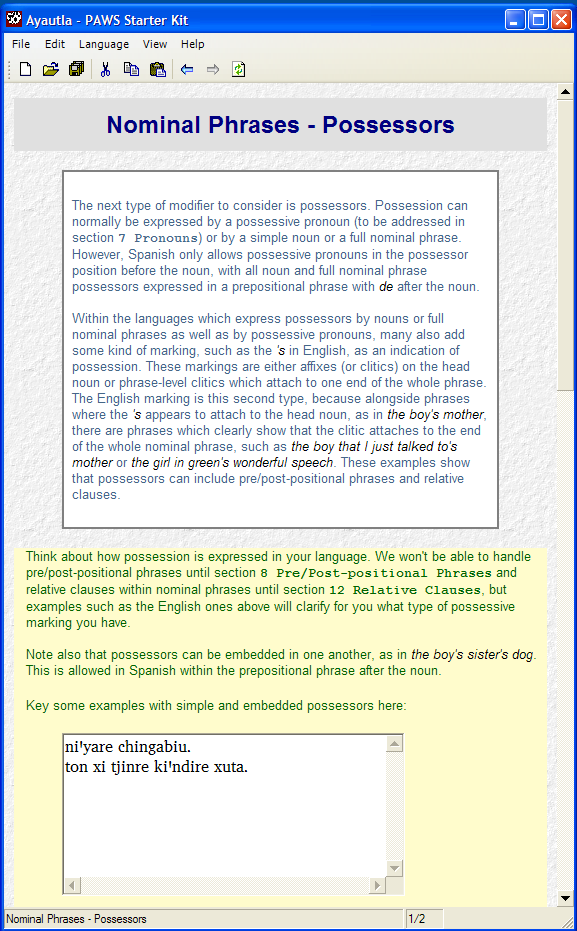
\includegraphics[width=\textwidth]{\imgpath/Possessors.png}
% \z
\begin{figure}[b]
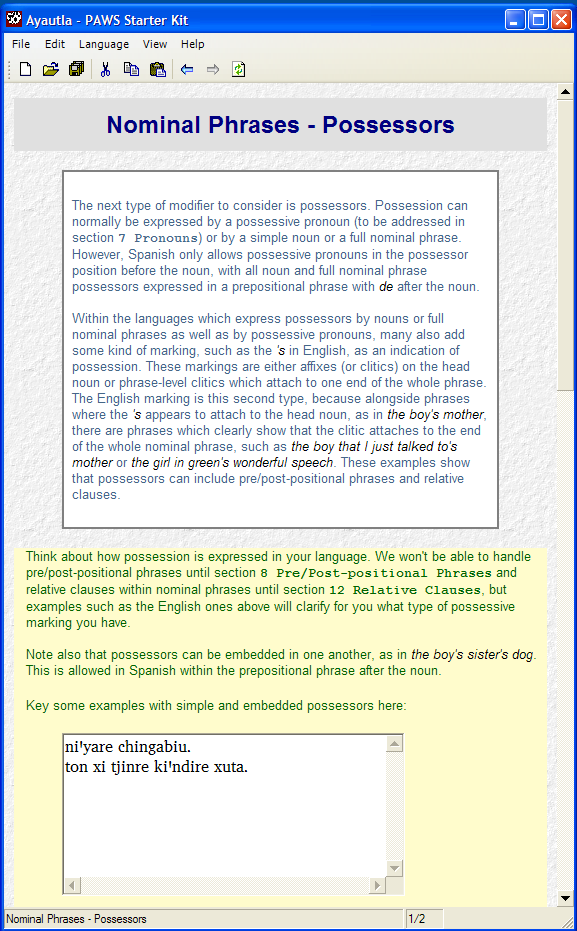
\includegraphics[height=.8\textheight]{\imgpath/Possessors.png} 
\caption{An instruction section along with a request to enter sample data}
\label{xPossesors1}%5
\end{figure}
  
\clearpage
% \newpage
% \ea  \label{xPossessor2}%6
% 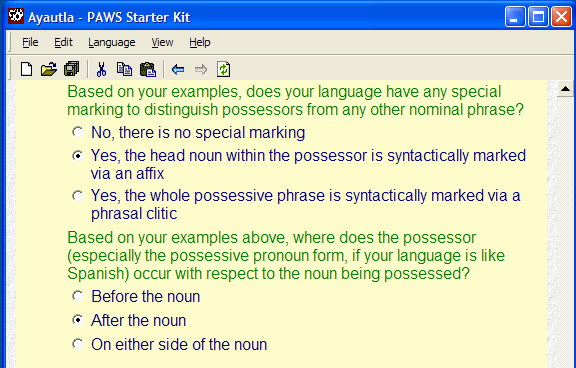
\includegraphics[width=\textwidth]{\imgpath/Possessors2a.png}
% \z
\begin{figure}[t]
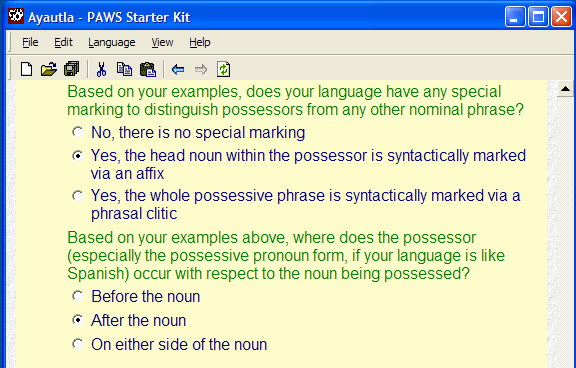
\includegraphics[width=\textwidth]{\imgpath/Possessors2a.png}
\caption{Two sets of multiple choice questions, followed by more instruction and a third multiple choice question.}
 \label{xPossessor2}%6
\end{figure}


\clearpage
% \ea  \label{xPossessor2c}%7
% 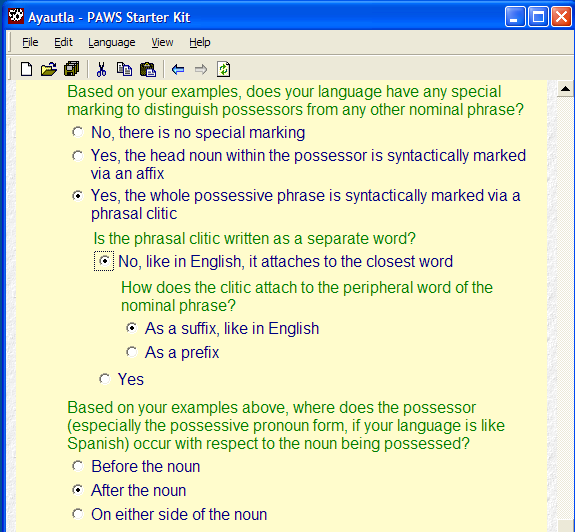
\includegraphics[width=\textwidth]{\imgpath/Possessors2c.png}
% \z
\begin{figure}[t]
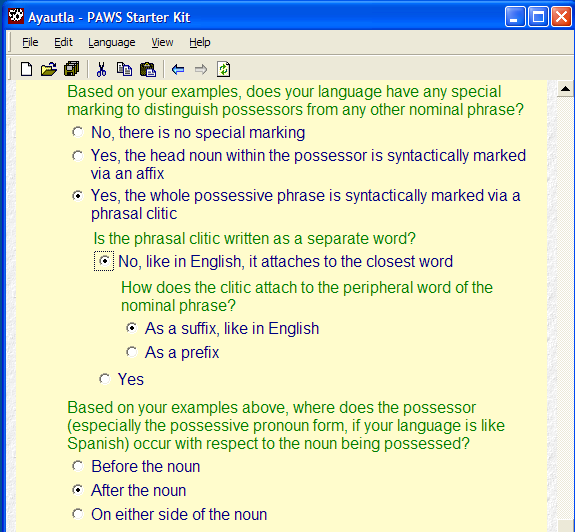
\includegraphics[width=\textwidth]{\imgpath/Possessors2c.png}
\caption{If a user clicks on the second "Yes" answer shown in Figure \ref{xPossessor2}, then more questions are asked (due to the fact that more information is needed about the nature of the phrasal clitic).}
 \label{xPossessor2c}%7
\end{figure}


\clearpage
% \ea  \label{xPossessors2b}%8
% 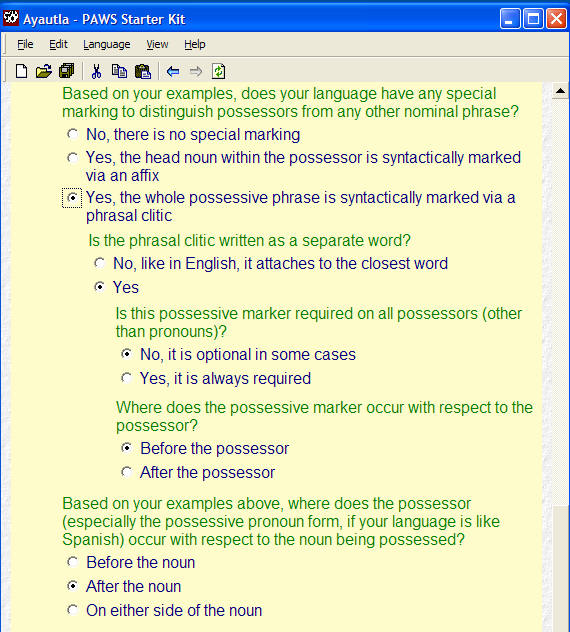
\includegraphics[width=\textwidth]{\imgpath/Possessors2b.png}
% \z
\begin{figure}[p]
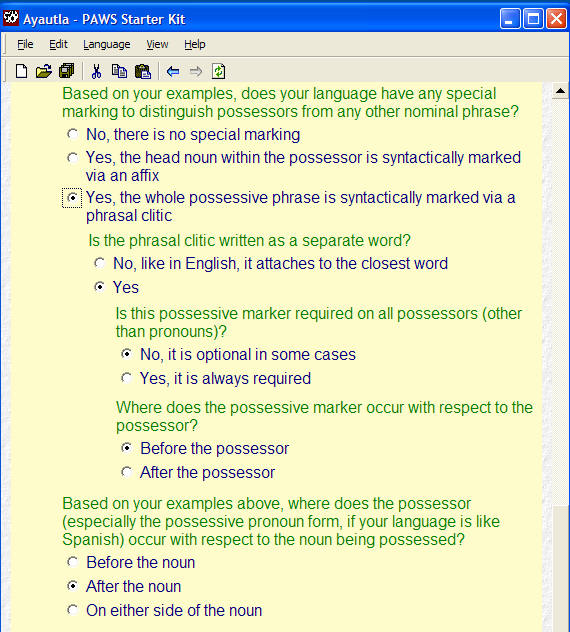
\includegraphics[width=\textwidth]{\imgpath/Possessors2b.png}
\label{xPossessors2b}%8
 \caption{If the user instead chooses the option to say that the phrasal clitic is written as a separate word, then even more questions appear.}
\end{figure} 

\clearpage
% \ea  \label{xPossessors3}%9
% 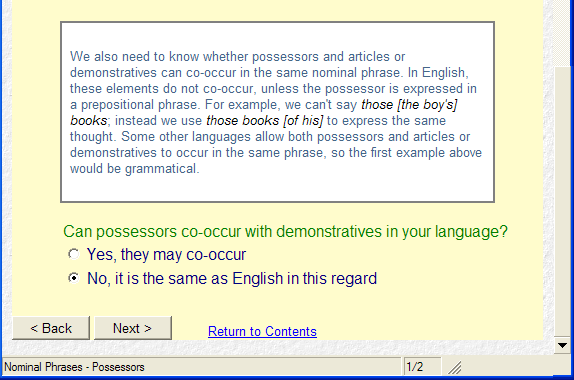
\includegraphics[width=\textwidth]{\imgpath/Possessors3aa.png}
% \z
\begin{figure}[p]
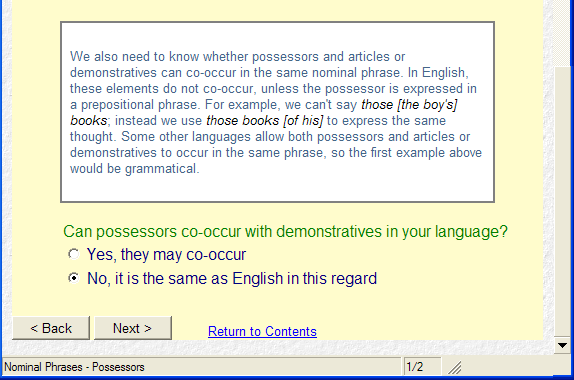
\includegraphics[width=\textwidth]{\imgpath/Possessors3aa.png}
\caption{The bottom portion of the page. It has some instruction, a question, and then two buttons, one for going back to the previous page and the other for going forward to the next page. It also has a link to jump to the main contents page.}
 \label{xPossessors3}%9
\end{figure} 
 \clearpage

\subsection{Grammar draft to edit}\label{sGrammar}
As the user works his/her way through these interactive pages, s/he can save their work and return later for another session. Whenever the work is saved, the output is produced based on the answers given so far. Naturally, we recommend that the user not look at the generated output until s/he has completed all the interactive pages.

Depending on the complexity of the language and how much data is entered, the draft of the practical grammar which is output could be about 60-90 pages if printed out. This includes the prose description and tables and interlinear data.

To illustrate the coverage of the practical grammar, the table of contents for the initial output of one grammar is shown in Figure \ref{xContents} \footnote{\label{nThirdLevelSections}
   In addition to the first and second level sections shown in \xref{xContents}, there are twenty four third level sections.
}

\begin{sidewaysfigure}
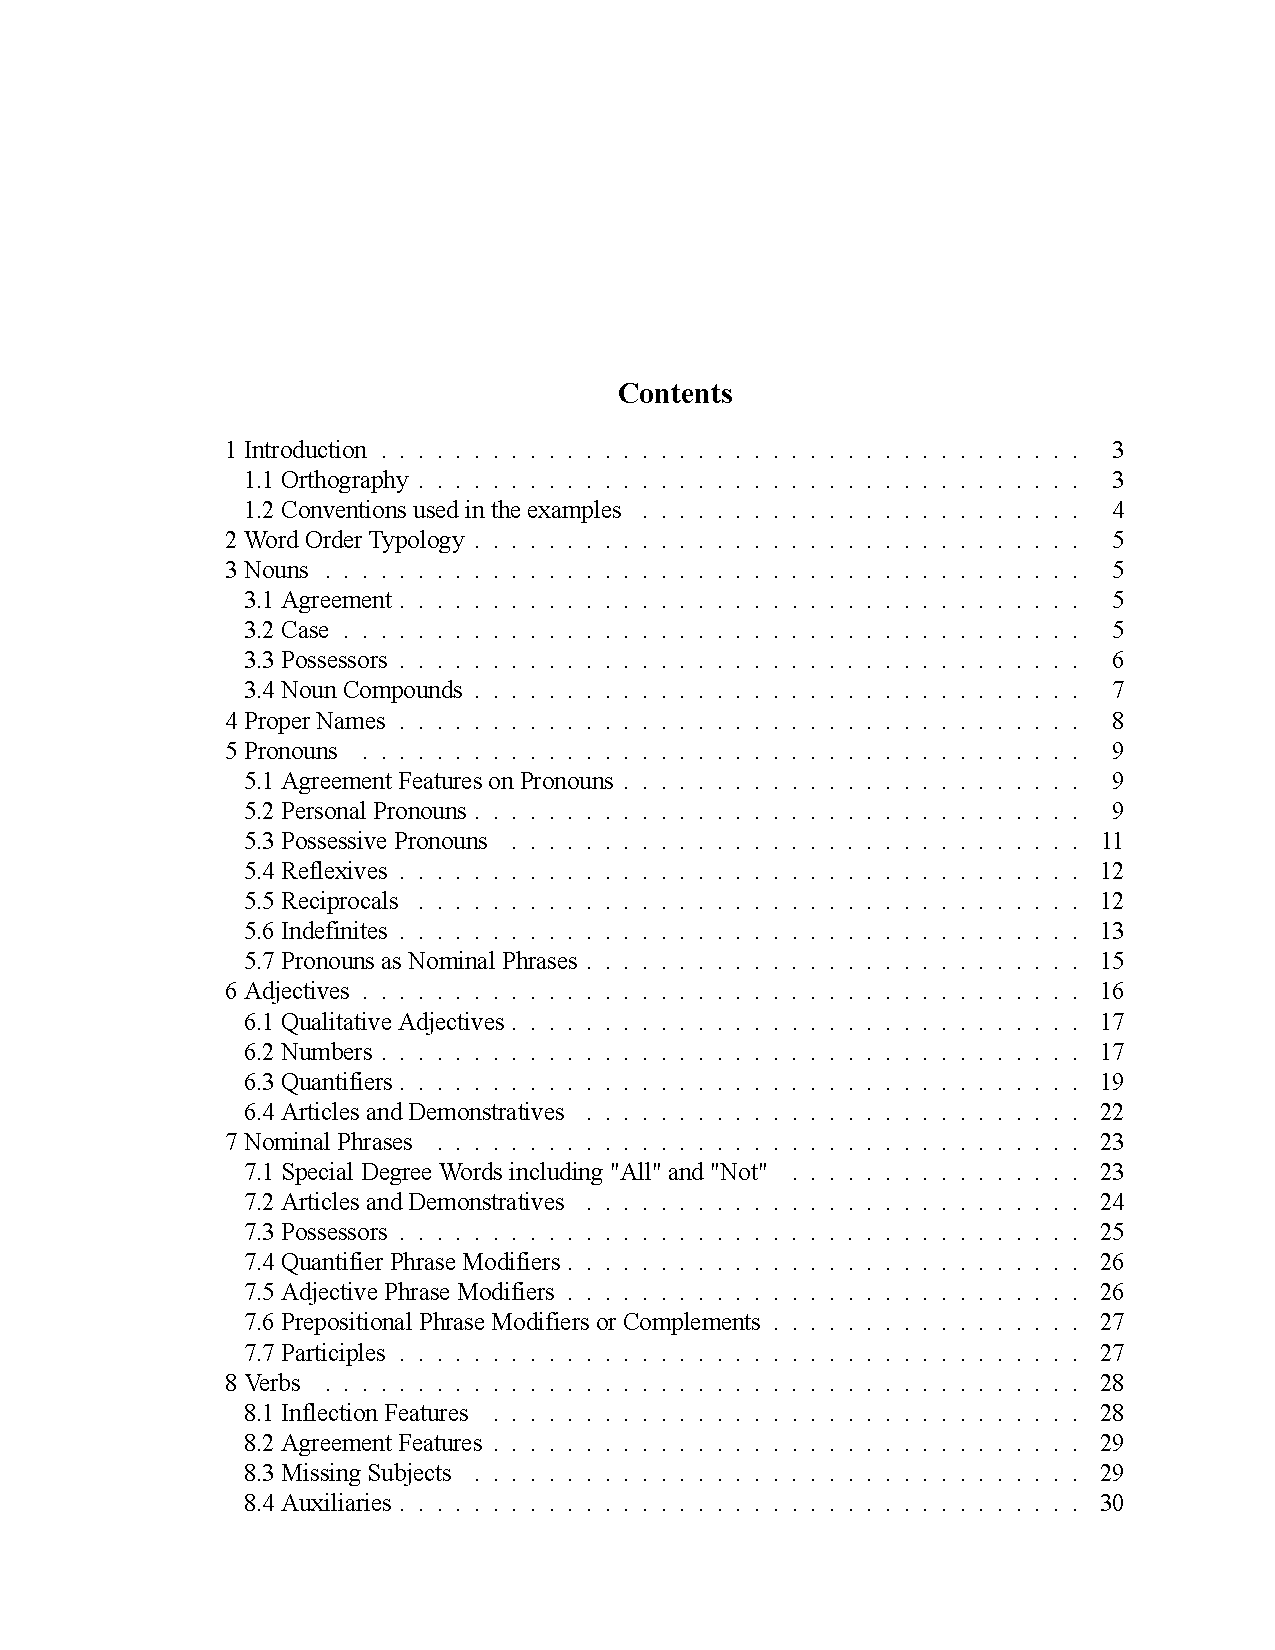
\includegraphics[width=.45\textwidth]{\imgpath/Contents1a.pdf}
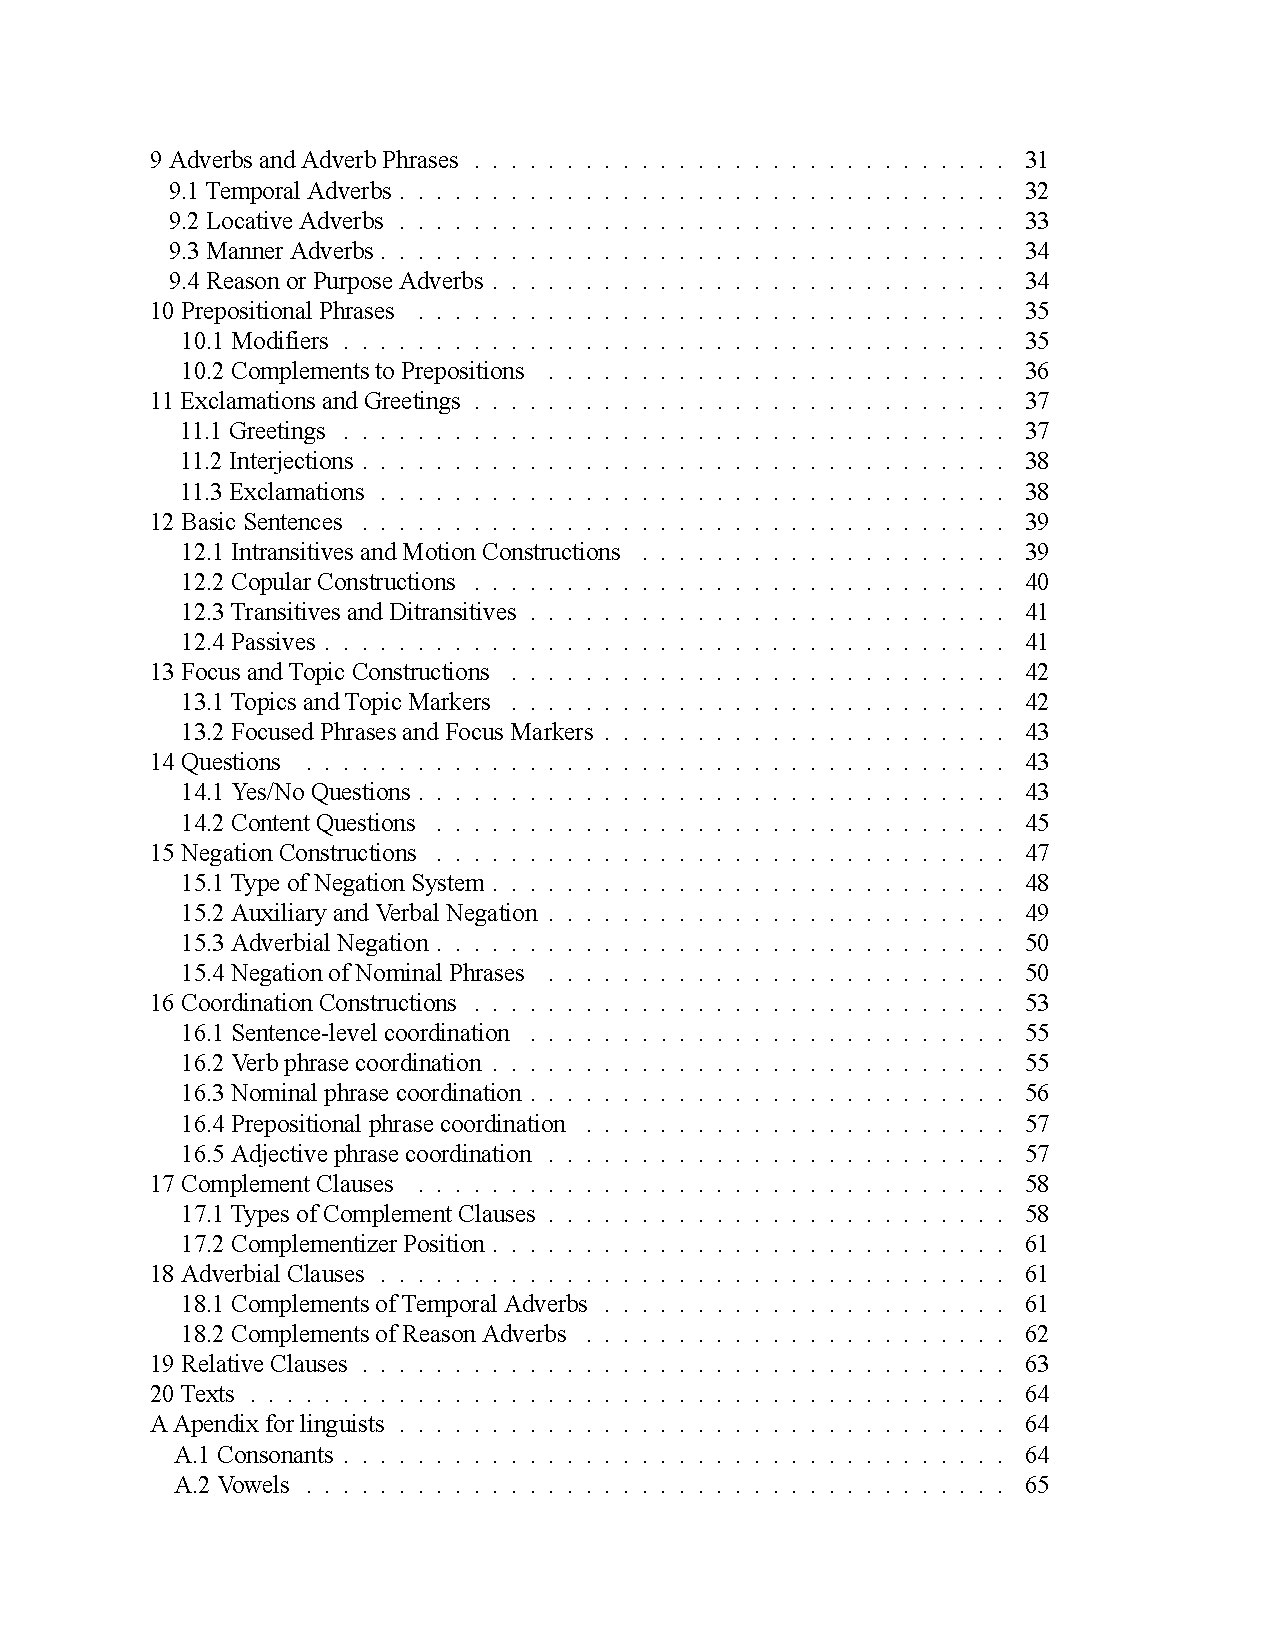
\includegraphics[width=.45\textwidth]{\imgpath/Contents2a.pdf}
\caption{Table of contents for the initial output of one grammar}
\label{xContents}%11
\end{sidewaysfigure}


\subsubsection{Use of XLingPaper}\label{sXLingPaper}
The practical grammar is output in XLingPaper format, which can then be edited as described in sections \ref{sXLingPaperOutputs}-\ref{sXMLMind}.  Before discussing this, we give a brief sketch of the advantages of XLingPaper.

Linguistic documents are by nature complex and also have many conventions. Using WYSIWYG editors like Microsoft Word and Open Officer Writer ``work'' but are not very convenient. As \citet{rSimonsAndBlackSFLF} point out, WYSIWYG editors are ``second wave'' technology. XLingPaper, on the other hand, uses ``third wave'' technology and is designed specifically for linguistic documents.

Linguists commonly face three obstacles in formatting papers. First, all examples are numbered in a paper. If during the writing process the author discovers a need to insert an example, then the numbering of all following examples and all references to those examples within the text need to be re-adjusted. This mechanical change can be both time-consuming and prone to error. Similarly, if the author decides to reorder some examples, then the numbering needs to be adjusted appropriately. XLingPaper provides an automatic way to facilitate such numbering and renumbering. 

Secondly, linguists cite the work of other researchers using a standard citation format. This format functions essentially as an abbreviation or reference to the full citation entry which appears in the references section of the paper. The burden of maintaining consistency between citation and reference typically falls totally on the author. Many a reader has been disappointed to find a citation to a paper in the body of a paper for which there is no entry in the references section. XLingPaper provides an automatic means for a writer to maintain consistency; all citations in the text must have a corresponding entry in the references. Conversely, XLingPaper will include only those entries in the references section which are cited in the text. This latter characteristic implies that one can maintain one master list of references and merely include it in any given paper. Only those references actually cited in the given paper will appear in the references section. 

Thirdly, linguists commonly use a set of abbreviations while glossing examples. They usually include either a list of the abbreviations and their definitions in a footnote, in a special front-matter page, or in a back-matter page. As for citations and references, the burden of maintaining consistency between the abbreviations used in the text and the abbreviations defined in the list typically falls totally on the author. Many a reader has been disappointed to find an abbreviation in a gloss for which there is no corresponding entry in the list of abbreviations. XLingPaper provides an automatic means for a writer to maintain consistency; the author can make it so all abbreviations in the text must have a corresponding entry in the list of abbreviations. Conversely, XLingPaper will include only those abbreviations in the list of abbreviations which are actually used in the text. This latter characteristic implies that one can maintain one master list of abbreviations\footnote{\label{nLeipzig}
   The starter master list which comes with XLingPaper is based on the Leipzig conventions given in  \url{http://www.eva.mpg.de/lingua/resources/glossing-rules.php}.
} 
and merely include it in any given paper. Only those abbreviations actually cited in the given paper will appear in the list of abbreviations. By the way, XLingPaper also creates a hyperlink between the abbreviation in the text and the abbreviation in the list of abbreviations. Thus, a reader can click on the abbreviation and see what it means.

Furthermore, XLingPaper  uses actionable data by marking-up linguistic documents in XML so one can produce multiple outputs from a single input.  As a brief example, the short section shown in Figure \ref{xSVCZSectionsXXE} is how a portion of one XLingPaper document appears in the {\XMLmindXMLEditor}.

\begin{figure}[h]
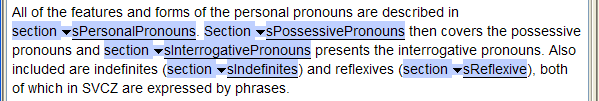
\includegraphics[width=\textwidth]{\imgpath/SVCZSectionsXXE.png}
\caption{A portion of an XLingPaper document in the {\XMLmindXMLEditor}}
  \label{xSVCZSectionsXXE}%12
\end{figure}

When this portion is formatted using the default PDF output format of XLingPaper, it looks like what is given in Figure \ref{xSVCZSectionsDefault}.
  
\begin{figure}[h]
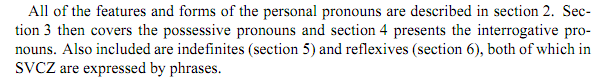
\includegraphics[width=\textwidth]{\imgpath/SVCZSectionsDefault.png}
\caption{Formatted pdf-output of the example in Figure \ref{xSVCZSectionsXXE}}
 \label{xSVCZSectionsDefault}%13
\end{figure}


When this sample document is associated with a publisher style sheet designed for submissions to the {\textit{International Journal of American Linguistics}} (see \citet{rIJALStyleSheet}), this portion will be formatted as in Figure \ref{xSVCZSectionsIJALSubmission}.  Notice that it is double-spaced and that the section numbers are in bold.

\clearpage
\begin{figure}[t]
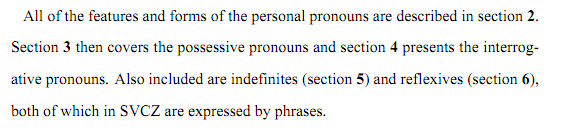
\includegraphics[width=\textwidth]{\imgpath/SVCZSectionsIJALSubmission.png}
\caption{Pdf-output of the example in Figure \ref{xSVCZSectionsXXE} formatted for \textit{IJAL}}
  \label{xSVCZSectionsIJALSubmission}%14
\end{figure}


 


When this sample document is associated with a publisher style sheet designed for the journal {\textit{Language}} (see \citet{rLanguageStyleSheet}), this portion will be formatted as in Figure \ref{xSVCZSectionsLanguage}. Notice that it is single-spaced in a smaller font size, the section numbers are in regular type face, and that rather than using the word ``section,'' it uses the section symbol §.

\begin{figure}[h]
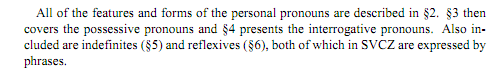
\includegraphics[width=\textwidth]{\imgpath/SVCZSectionsLanguage.png}
\caption{Pdf-output of the example in Figure \ref{xSVCZSectionsXXE} formatted for \textit{Language}}
 \label{xSVCZSectionsLanguage}%15
\end{figure}

 

The three different outputs shown in Figures \ref{xSVCZSectionsDefault}-\ref{xSVCZSectionsLanguage} are all produced without any changes to the main content of the XLingPaper document.  This shows the power of using actionable data.\footnote{\label{nXLingPaperPowerOfActionableData}
   For more on this, see the demonstration movie ``The Power of Actionable Data" on the XLingPaper web site, \url{http://www.xlingpaper.org/?page\_id=14}.
}

XLingPaper works natively on Windows, Mac OS X, and Linux operating systems.\footnote{\label{nXXEOSes}
   This is largely due to the fact that the {\XMLmindXMLEditor} runs natively on these operating systems.
}  
An XLingPaper document can be output in any of five formats:

\begin{itemize}
  \item {Web page (html)}
  \item {PDF (via XeLaTeX; see \url{http://scripts.sil.org/cms/scripts/page.php?site_id=nrsi&id=xetex})}
  \item {PDF (via RenderX; see \url{http://www.renderx.com/})}
  \item {Microsoft Word 2003}
  \item {Open Office Writer}
\end{itemize}

Those who have used XLingPaper have said things like the following quotes:

\begin{itemize}
  \item ``I'm totally hooked on this program now and am generally getting quite comfortable using it.''
  \item It ``has enabled me to be vastly more productive in writing linguistic papers and in dialoguing with linguistic consultants.''
  \item ``I really like using XLingPaper.  It's a much better working space for me than MS Word (partly because I have spent so much time not being productive, in Word, and because of the intimidation of the blank page.)''
  \item ``XLingPaper has been working great, and I've been using it to author \dots{} most of what I write.''
\end{itemize}

To see some sample papers produced via XLingPaper, see Working Papers \# 1, 3, 4, 7, 8, 9, 10, and 13 at \url{http://www.sil.org/mexico/workpapers/WPindex.htm}.

While XLingPaper is a powerful authoring tool for linguistic documents, the user of {PAWS} does not have to learn everything about XLingPaper before s/he can begin editing. This is because {PAWS} already formats the sections, interlinear examples, and tables so that the user only has to key in the glosses or other additional information requested. Further, adding additional description or interlinear examples or tables can be done by simply copying and pasting similar ones already in the document.

\subsubsection{XLingPaper outputs}\label{sXLingPaperOutputs}
As we just mentioned, the output is in XLingPaper format, which allows editing within XML editors, and produces outputs in both HTML (\citet{rW3CHTML} and PDF (\citet{rISOPDF1.4} formats. {PAWS} automatically generates the HTML output for the user's convenience.

The HTML output page corresponding to the input page from Figures \ref{xPossesors1}-\ref{xPossessors3} 
% of section \ref{sPages} 
is shown in Figure \ref{xPossessorsHtml2}.

\begin{figure}
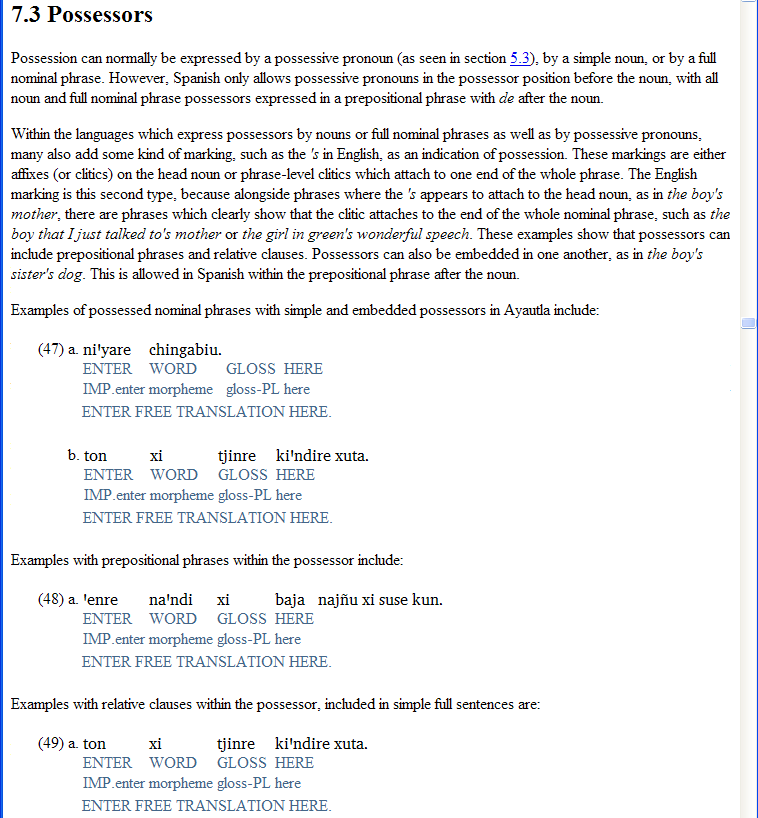
\includegraphics[width=\textwidth]{\imgpath/PossessorsHtml1.png} 
...\\[1em]
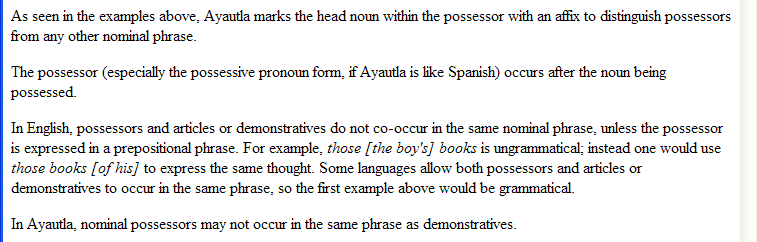
\includegraphics[width=\textwidth]{\imgpath/PossessorsHtml2.png}
\caption{HTML output of the content of Figures  \ref{xPossesors1}-\ref{xPossessors3}}
  \label{xPossessorsHtml2}%17
\end{figure}

While {PAWS} only generates the HTML output, XLingPaper allows for multiple possible PDF outputs.

\subsubsection{{\XMLmindXMLEditor}}\label{sXMLMind}
We have found that using XLingPaper with the {\XMLmindXMLEditor} is the most convenient.\footnote{\label{nXXE}
   See \url{http://www.xmlmind.com/xmleditor/} for more on this exceptional structured editor.
} 
This is because the {\XMLmindXMLEditor} hides the XML from the user. In addition, the XLingPaper configuration files for the {\XMLmindXMLEditor} provide many other capabilities that makes it convenient for the author.

What the user sees within the {\XMLmindXMLEditor} for the first part of the same page we illustrated above in Figures \ref{xPossesors1}-\ref{xPossessors3} is given in Figure \ref{xXXE1}.

\clearpage
\begin{figure}[h]
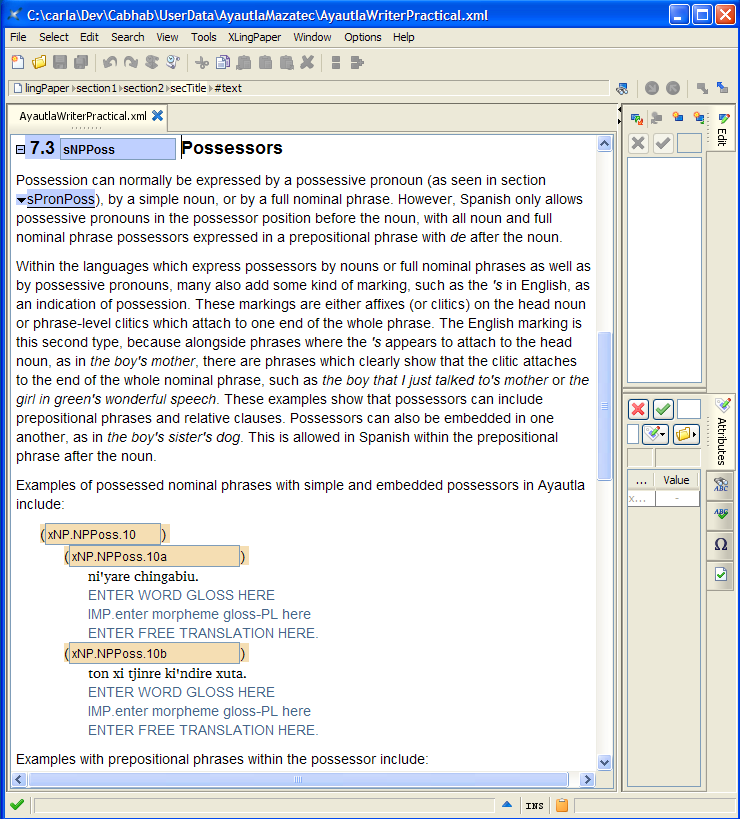
\includegraphics[width=\textwidth]{\imgpath/XXE2.png}
\caption{Screenshot of the {\XMLmindXMLEditor}}
\label{xXXE1}%18
\end{figure}
\clearpage
The section level 2 item begins the portion, followed by several paragraphs of descriptive prose. It ends with two sets of interlinear examples. These have the four lines discussed in section \ref{sPracticalStructure}. The editor allows the user to type in the information asked for in blue, as well as to add additional data and/or prose as appropriate.

\section{How it works}\label{sComp}
Having described what {PAWS} entails, we turn now to describing how it works. 


\subsection{The configuration files}\label{sConfig}
The {PAWS} program consists of a shell or host program (called \textsc{cabhab}) which has an embedded web browser and also processes a set of configuration files. These files determine the user interface such as menu items, define sets of transforms to apply to the answer file, and also determine what shows in the embedded web browser.

There are several sets of configuration files. 

\subsubsection{Controlling the shell}\label{sConfigCabhab}
There is a configuration file that controls what the {cabhab} shell shows the user and also how the answer file is transformed into various outputs.

For example, the menu items are defined as shown in \xref{xConfigMenuItems}.

\ea  \label{xConfigMenuItems}%19
\begin{verbatim}
<menubar>
   <menu id="File" label="File">
      <item command="CmdNewLanguage" defaultVisible="true"/>
      <item command="CmdOpenLanguage"/>
      <item command="CmdCloseLanguage"/>
      <item command="CmdSaveLanguageAs"/>
      <item label="-"/>
      <item command="CmdGenerateFiles"/>
      <item label="-"/>
      <item command="CmdLanguageFileLocations"/>
      <item label="-"/>
      <item command="CmdExit"/>
   </menu>
   <menu id="Edit" label="Edit">
      <item command="CmdCut"/>
      <item command="CmdCopy"/>
      <item command="CmdPaste"/>
      <include path="Extensions/*/MainConfigurationExtension.xml" 
        query="root/menuAddOn/menu[@id='Edit']/*"/>
   </menu>
   <menu id="Language" label="Language">
      <item command="CmdLanguageProperties"/>
      <item command="CmdLanguageFileLocations"/>
      <include path="Extensions/*/MainConfigurationExtension.xml" 
        query="root/menuAddOn/menu[@id='Edit']/*"/>
   </menu>
   <menu id="View" label="View">
      <item label="Show Toolbar" boolProperty="ShowToolbar" 
            command="CmdShowToolbar"/>
      <item label="Show Status Bar" boolProperty="ShowStatusBar"
            command="CmdShowStatusBar"/>
      <item label="-"/>
      <item command="CmdBack"/>
      <item command="CmdForward"/>
      <item command="CmdRefresh"/>
   </menu>
   <menu id="Help" label="Help">
      <item id="Resources" command="CmdResources"/>
      <item label="-"/>
      <item id="About" command="CmdAbout"/>
   </menu>
</menubar>
\end{verbatim}
\z

 The commands referred to by <item> elements are defined in the configuration file as given in example \xref{xConfigCommands}.

\ea  \label{xConfigCommands}%20
\begin{verbatim} 
<commands>
   <command id="CmdNewLanguage" label="Create _New 
            Language" shortcut="Ctrl+N" 
            message="NewLanguage" icon="New"/>
   <command id="CmdOpenLanguage" label="Open Language" 
            message="OpenLanguage" shortcut="Ctrl+O" 
            icon="Open"/>
   <command id="CmdCloseLanguage" label="Close Language" 
            message="CloseLanguage"/>
   <command id="CmdGenerateFiles" label="Generate Files"
            message="GenerateFiles" shortcut="Ctrl+S" 
            icon="Save"/>
   <command id="CmdSaveLanguageAs" label="Save Language 
            As" message="SaveLanguageAs"/>
   <command id="CmdExit" label="E_xit" 
            message="ExitApplication"/>
   <command id="CmdCopy" label="Copy" message="EditCopy" 
            icon="Copy" shortcut="Ctrl+C"/>
   <command id="CmdCut" label="Cu_t" message="EditCut" 
            icon="Cut" shortcut="Ctrl+X"/>
   <command id="CmdPaste" label="Paste" message="EditPaste" 
            icon="Paste" shortcut="Ctrl+V"/>
   <command id="CmdLanguageProperties" label="Properties" 
            message="LanguageProperties"/>
   <command id="CmdLanguageFileLocations" label="File _Locations" 
            message="LanguageFileLocations"/>
   <command id="CmdBack" label="Back" message="BrowserBack" 
            icon="Back" shortcut="Alt+Left"/>
   <command id="CmdForward" label="Forward" message="BrowserForward" 
            icon="Forward" shortcut="Alt+Right"/>
   <command id="CmdRefresh" label="Refresh" message="BrowserRefresh" 
            icon="Refresh" shortcut="F5"/>
   <command id="CmdAbout" label="About PAWS" message="AboutPage"/>
   <command id="CmdResources" label="Resources" 
            message="ResourcesPage"/>
   <command id="CmdShowToolbar" label="Show Toolbar" 
            message="ShowToolbar"/>
   <command id="CmdShowStatusBar" label="Show Status Bar" 
            message="ShowStatusBar"/>
</commands>
\end{verbatim}
\z


 The message attribute refers to code in the {cabhab} program which is run when that command is invoked.

 The set of transforms which are used to produce the various outputs are defined as illustrated in example \xref{xConfigAnswerFileTransforms}. Only the one for the practical grammar output (in English) is shown. The others are similar.

\ea  \label{xConfigAnswerFileTransforms}%21
\begin{verbatim}
 
<answerFileTransformSets>
   ...
   <answerFileTransformSet>
      <transform 
        file="Transforms/PAWSSKMasterWriterPracticalMapper.xsl"
        resultFileFromAnswerFile="//language/writerPracticalFile" 
        ext="xml" saveResult="true"
        applyTransformWhenXPath=
            "/paws/\@outputWriterPractical[.='True']"
        insertConfigPathInTransformDOCTYPE="true" 
        replaceDOCTYPE="&lt;!DOCTYPE 
        lingPaper PUBLIC &quot;-//XMLmind//DTD XLingPap//EN&quot; 
        &quot;XLingPap.dtd&quot;&gt;" lang="en">
         <xsltParameters>
            <param name="prmSDateTime" value="fake"/>
            <param name="prmSVersionNumber" value="fake"/>
         </xsltParameters>
      </transform>
      <transform file="Transforms/XLingPap1.xsl" 
        resultFileFromAnswerFile="//language/writerPracticalFile" 
        ext="htm"
        applyTransformWhenXPath=
            "/paws/@outputWriterPractical[.='True']"/>
   </answerFileTransformSet>
   ...
</answerFileTransformSets>
\end{verbatim}
\z

\subsubsection{Web page description}\label{sConfigWebPage}
The second set of configuration files are the web page descriptions. The development of each web page used in PAWS was done by a non-programmer linguist, who wrote XML files describing the content of the page. Example \xref{xSamplePageDescription} shows a portion of the XML description used to produce the page shown in Figures \ref{xPossesors1}-\ref{xPossessors3}.

\ea  \label{xSamplePageDescription}%22
\begin{verbatim}
<page id="NPPossessors" count="1/2">
   <title level="2">Nominal Phrases - Possessors</title>
   <introduction> 
      The next type of modifier to consider is 
      possessors. Possession can normally be expressed by a
      possessive pronoun (to be addressed in <section 
      number="7">Pronouns</section>) or by a simple noun... 
      a prepositional phrase with <example>de</example> 
      after the noun.<br/>... These examples show that 
      possessors can include pre/post-positional phrases 
      and relative clauses. 
    </introduction>
   <form section="np">
      <prompt>
        Think about how possession is expressed in your
        language. ...
      </prompt>
      <prompt> 
        Key some examples with simple and embedded 
        possessors here:
      </prompt>
      <textBox id="NPPossEmbeddedExample"
               dataItem="embeddedExample"/> 
       <radioGroup>
         <groupName dataItem="possMarked" default="no">
          RNPPossMarked
         </groupName>
         <prompt>
            Based on your examples, does your language have 
            any special marking to distinguish possessors 
            from any other nominal phrase?
         </prompt>
         <radio id="NPPossMarkedNo" dataValue="no">
            No, there is no special marking
         </radio>
         <radio id="NPPossMarkedYesAffix" dataValue="yesAffix">
            Yes, the head noun within the possessor is 
            syntactically marked via an affix
         </radio>
         <radio id="NPPossMarkedYesClitic" dataValue="yesClitic">
            Yes, the whole possessive phrase is syntactically 
            marked via a phrasal clitic
          </radio>
         ...
      </radioGroup>
   </form>
</page>

\end{verbatim}
\z

An XSLT transform then produces the web page itself on the fly while the user is running {PAWS}.

\subsubsection{Writer output description} \label{sConfigWriterOutput}
  
The next set of configuration files describes a given writer output.

The writer output was developed similarly: the linguist described the desired output in XML and then this XML was transformed into the XSLT that {PAWS} uses. For example, the portion of XML shown in \xref{xPossessorPracticalWriter} shows part of what ends up producing the kind of output given in Figure \ref{xPossessorsHtml2}.\footnote{\label{nContentElement}
   The use of the <content> element instead of plain PCDATA is a result of how the XSLT to transform this XML to XSLT was written: if one used PCDATA, the resulting XSLT would be incorrect.
}

\ea  \label{xPossessorPracticalWriter}%23
\begin{verbatim}
<section2 id="sNPPoss"> 
   <secTitle>Possessors</secTitle> 
   <p> 
      <content>
          Possession can normally be expressed by a 
          possessive pronoun (as seen in section 
      </content> 
      <sectionRef sec="sPronPoss"/> 
      <content>
          ), by a simple noun, or by a full nominal 
          phrase. However, Spanish only allows 
          possessive pronouns in the possessor 
          position before the noun, with all noun 
          and full nominal phrase possessors expressed 
          in a prepositional phrase with 
      </content>
      <langData>de</langData> 
      <content> after the noun.</content> 
   </p>
   ... 
   <p> 
      <content>
          Examples of possessed nominal phrases with 
          simple and embedded possessors in 
      </content>
      <langName/>
      <content> include:</content>
   </p> 
   <example>
      <interlinear exampleLoc="np/embeddedExample"/>
   </example> 
   ... 
   <p> 
   <content>As seen in the examples above, </content>
      <langName/>
   <content/> 
   <case element="np" attr="possMarked"> 
      <caseText value="no"> 
          does not have any special marking to 
          distinguish possessors from any other nominal 
          phrase.
      </caseText> 
      <caseText value="yesAffix"> 
          marks the head noun within the possessor with 
          an affix to distinguish possessors from any 
          other nominal phrase.
      </caseText> 
      <caseText value="yesClitic"> 
          marks the whole possessive phrase with a phrasal 
          clitic to distinguish possessors from any other 
          nominal phrase.
      </caseText>
   </case>
   <content/> 
\end{verbatim}
\z

\subsection{Process for producing writer output}\label{sProcessProducingWriterOutput}
The overall process for producing the writer output is illustrated in Figure \ref{xWriterToOutput}.

\begin{figure}
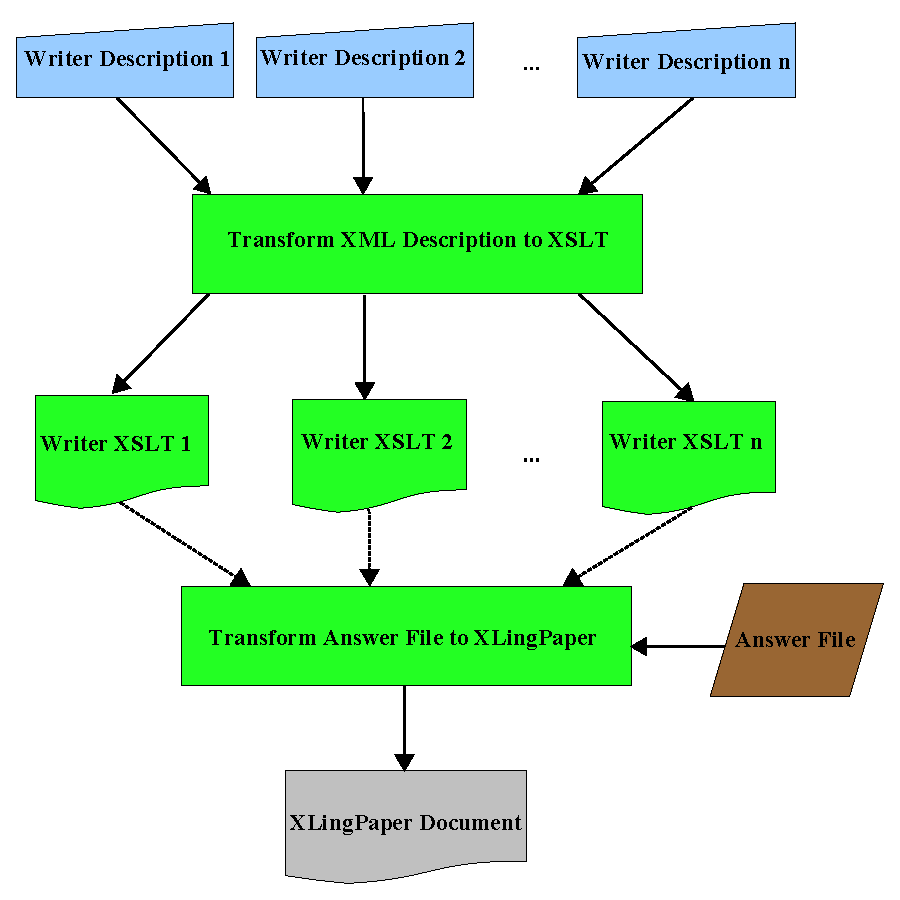
\includegraphics[width=\textwidth]{\imgpath/WriterXMLtoXSLFlow3NewText.pdf}
\caption{Process of producing XLingPaper} 
 \label{xWriterToOutput}%24
\end{figure}

The linguist writes several writer description XML files, each of which must conform to a Document Type Definition \citep[also known as a DTD; see ][]{rW3CDTD}. Each such file typically describes a section or a sub-section of the intended output. Each of these writer description files is then passed through an XSLT transform to produce the corresponding writer XSL file.\footnote{\label{nWriterToXSLDoneOnce} 
 This is done only once during the development process. The individual writer XSL files are then included in the installation package as part of {PAWS}.
} 
These are combined together in the master XSLT writer transform. The PAWS program then applies the answer file to this combined transform to produce the XLingPaper document output.

\subsection{Choice of outputs} \label{sOutputs}
As noted above in section \ref{sPages}, through the use of actionable data, a single set of answers to questions and example data that the user enters can provide either a PC-PATR grammar file and test data for syntactic parsing or a choice of two styles of a grammar write-up.

This grammar write-up is an XML file in XLingPaper format, so it is ready for electronic publishing.\footnote{\label{nMukurtu}
 One reviewer of an earlier version of this paper mentioned the Mukurtu repository system (see \url{http://www.mukurtu.org/}). One could easily put the output of the edited XLingPaper result of {PAWS} on such a site. Another reviewer noted that a wiki rather than XML would be a possible target for a language community. We acknowledge this possibility with thanks. Since XLingPaper data is actionable, it is at least conceivable that one could create an XSLT transform that would convert the XLingPaper XML document to wiki pages. One could then post these pages to a wiki site, enabling the language community to refine the result.
} 
See examples in section \ref{sXLingPaper} above.

\subsection{Localization}\label{sLocal} 
The original grammar write-up included in PAWS closely follows the order and style of the user interface pages within PAWS, so it is a descriptive, pedagogical grammar comparative to English. This has been customized with the addition of the option of producing a practical grammar style write-up. Currently, the practical grammar is available in English and in Spanish. The process of translating the practical grammar output involves making a new copy of the XML writer description files, such as the one shown in \xref{xPossessorPracticalWriter}, and translating the text.

SIL International uses such practical grammars in Mexico, written in Spanish. (See \citet{rHollenbach} as well as \citet{rPickettBlackMarcial} and \citet{rPersonsBlack} for examples.) Therefore, the practical grammar option has been translated into Spanish and the translation of the user interface is in process, to allow greater use throughout the Spanish-speaking world. Similar localization for other languages could be done in the future.

Additional customization is possible by the user (with configuration files to generate a transform), since PAWS employs XML technologies.

\section{Conclusion}\label{sConc}
This paper has shown how using XML technologies to produce an expert system allows PAWS to meet multiple needs and produce multiple outputs. While originally developed for syntactic parsing, it can also be used to produce practical grammars, with the more complex instructions hidden from the user. This practical grammar option, especially coupled with localization into the national language, allows linguistically-aware native speakers of indigenous languages to partner with linguists in the task of documenting and describing the minority languages of the world and providing useful grammars for each language community.

Workshops on grammar writing are much more productive by beginning with PAWS. In such workshops, the participants all complete PAWS and then are taught how to edit the output using XLingPaper. From then on, the workshop can move to dealing with any language-specific phenomena not covered in PAWS. The participants can be taught how to search for the needed data, how to analyze it and then how to write it up in the grammar.

Though the grammar drafts output by PAWS have a template-like quality, they are simply a big head start on writing the grammar. After editing and enhancing the grammar using XLingPaper, a unique description of the particular language can be produced.

\setcounter{secnumdepth}{3}

\documentclass{article}
\usepackage[utf8]{inputenc} % please use UTF8 encoding
\usepackage[T1]{fontenc} 
\usepackage{gb4e}

\begin{document} 
% This file was converted to LaTeX by Writer2LaTeX ver. 1.0.2
% see http://writer2latex.sourceforge.net for more info
\documentclass[letterpaper]{article}
\usepackage[ascii]{inputenc}
\usepackage[T3,T1]{fontenc}
\usepackage[english]{babel}
\usepackage[noenc]{tipa}
\usepackage{tipx}
\usepackage{amsmath}
\usepackage{amssymb,amsfonts,textcomp}
\usepackage[top=0.4917in,bottom=0.7874in,left=0.9839in,right=0.9839in,includehead,head=0.4925in,headsep=0.4528in,nofoot]{geometry}
\usepackage{array} 
\usepackage{hhline}
\usepackage{hyperref}
\hypersetup{colorlinks=true, linkcolor=blue, citecolor=blue, filecolor=blue, urlcolor=blue}
\usepackage{graphicx}
\begin{document}
\clearpage\setcounter{page}{1}\pagestyle{Standard}

\end{document}


\end{document}



\glossSTDmode
\setcounter{exx}{0}\setcounter{footnote}{0}
\renewcommand{\imgpath}{/Bouda/.}
\newpage
\renewcommand{\thischapteruuheader}{\uhheader{129-159}{4533}}
 
\renewcommand\chapname{From corpus to grammar}	
\renewcommand\longchapname{From corpus to grammar: how DOBES corpora can be exploited for descriptive linguistics}
\renewcommand\shortauthor{Peter Bouda and Johannes Helmbrecht}
\renewcommand\longauthor{Peter Bouda$^\spadesuit$ and Johannes Helmbrecht$^\heartsuit$\\
$^\spadesuit$Ludwig-Maximilians-Universität München,  $^\heartsuit$Universität Regensburg}
\chapter*{\longchapname}
\chapterauthor{\longauthor}
\mytoc{}
 
 
\begin{abstract}
The principles and techniques of language documentation developed during the last one and half decades and the sheer amount of corpora which have been compiled for endangered languages up to now will have an impact on grammar writing in particular with respect to the data base of grammars.  On the other hand, advances in computer technology allow a closer link between corpus data which are the basis for generalizations and the grammatical description itself. The future the grammatical description of a language will not only present selected illustrative examples, but will also be linked to the entire set of corpus data that are the empirical basis for it. This makes generalizations transparent to the reader and open to falsification by the scientific community.

The article critically examines the relations between the DOBES corpus, the analysis and the grammatical description itself. Special attention will be laid on the   particular the two fundamental perspectives of a semasiological and an onomasiological grammar, can be translated into the various kinds of search and concordancing routines to be executed in the corpus analysis. We present a typology of searches descriptive linguists need to apply. This typology defines requirements with regard to the functionality of specific software to be developed.
In the second part, the article presents a technical solution, a preliminary version of a database/concordancing software specifically designed to fulfill the functions and principles outlined in the preceding sections.
\end{abstract}


\section{Introduction}

Right now, there are about 50 DOBES projects documenting endangered languages around the world (cf. the DOBES map below).

\begin{figure}
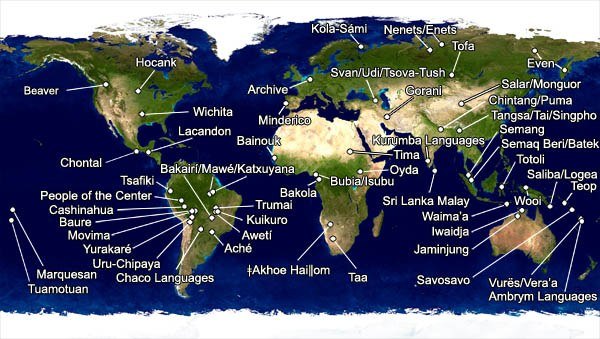
\includegraphics[width=\textwidth]{.\imgpath/Bouda-img7.jpg}
\caption{The DOBES documentation projects \url{http://www.mpi.nl/dobes}}
\end{figure}


Language documentation is a multi-purpose enterprise, but one important purpose of DOBES corpora is to serve as data bases for grammatical descriptions of these languages. Since these corpora have a different structure and different properties than the large monolingual corpora that are available for English, German and other major European languages they allow for and require different corpus linguistic methods. Or, to put it the other way round, corpus linguistic methods have to be adapted to the specific properties of DOBES corpora.

One of the great advantages of DOBES corpora over these traditional corpora is that they are always bilingual with an idiomatic translation in one of the main European languages, and in addition, that they often include a morpheme-by-morpheme glossing. This means that DOBES corpora contain much more additional information in form of these types of annotations than traditional corpora. The large monolingual corpora mostly consist of plain text only. It is the overall goal of this article to show how corpora such as DOBES corpora can be exploited by corpus linguistic means in order to extract the kind of data that are necessary for grammatical descriptions. 

What kind of data is necessary for a grammatical description can be deduced from the principles and requirements of grammaticography. One important distinction that is maintained in grammaticography is the one between a semasiological and an onomasiological approach to grammar. 

The semasiological approach takes the formal expressions of a language as starting point and tries to find out what they mean in different contexts. This approach resembles the analytic tasks hearers have to fulfill in interpreting speakers' utterances. They have to start from the uttered expression and have to assign a meaning to them which is appropriate in the given shared context of the utterance. 

The onomasiological approach, on the other hand, takes the meaning/ function as starting point and tries to find out which forms in a language may be used to express them. This approach resembles the generative task the speaker has to fulfill in order to form an utterance. The speaker has a concept of what he/she wants to communicate to the hearer and his/her task is to find the appropriate expression in a given shared context that fulfills the intended meaning best.

These different but complementary approaches to grammar have also an impact on the data searching methods to be applied to the corpus. The semasiological approach dominates in traditional computational treatments of monolingual text corpora. Specific lexical or grammatical forms in the target language are searched for in digital corpora. The goal is to collect all different contexts in which these forms appear in order to find out the conventional meanings of these forms and their variation in different contexts. 

The onomasiological approach, on the other hand, requires a semantic annotation such that all forms and constructions that express a certain semantic notion -- for instance possession -- are annotated in a way that the search for the annotation ``possession'' gives all different expressions of this notion. A semantic annotation is -- of course - the rare exception in digital corpora, since they have to be added manually, which is a quite time-consuming process. 

It is one of the main goals of this paper to show that the particular strength of DOBES corpora is that they can be exploited much more systematically than traditional monolingual corpora. They allow for searches that provide the necessary data for both the semasiological and the onomasiological approach in direct and indirect ways. The second goal of this paper is to present a linguistic database and concordancing software -- the Poio Analyzer - that allows easily - i.e. in a user friendly manner -- to conduct the text searches that are necessary to extract the kinds of data from a DOBES corpus that are required for the two different analytical approaches to grammar just mentioned. 

The structure of the paper is as follows. The main properties of DOBES corpora and their implications for the various search types will be dealt with in Section\ \ref{bouda:sec:structureandproperties}. Section\ \ref{bouda:sec:typologyofsearches} presents a general typology of possible search types within DOBES corpora. These search types are -- in principle -- independent of the two approaches to grammar and the types of data they require. It will be demonstrated that these kinds of searches exceed the possibilities that monolingual corpora allow for. In Section\ \ref{bouda:sec:structuralgrammar}, it will be exemplified how these search types can be utilized to gain data that are relevant for a semasiological description. In Section\ \ref{bouda:sec:functionalgrammar}  in turn, it will be exemplified how data may be extracted from a DOBES corpus - using these search types - that are relevant for the onomasiological description. In Section\ \ref{bouda:sec:softwarebasesearch}  and Section\ \ref{bouda:sec:poioanalyzer}, the functionality and the shortcomings of Elan with regard to concordances will be evaluated and the prototype of a linguistic database and concordancing software -- the Poio Analyzer - will be introduced that is designed specifically for the needs of a descriptive linguist.

\section{The structure and properties of DOBES corpora}%\label{bkm:Ref283033309}
\label{bouda:sec:structureandproperties}
The typical structure of an annotated text of a DOBES corpus can be seen in Figure  \ref{bouda:fig:corpussentence}. An annotated text consists minimally: a) of a text tier (abbreviated \textit{tx} in Figure \ref{bouda:fig:corpussentence}) containing the transcribed text of the audio and video recording, and b) a free idiomatic translation tier (abbreviated \textit{ft} in Figure  \ref{bouda:fig:corpussentence}). Many DOBES corpora have, in addition, a morpheme-by-morpheme glossing such that there is c) a tier with a morpheme segmentation (abbreviated \textit{mo} in Figure  \ref{bouda:fig:corpussentence}) and d) a tier with lexical and grammatical glosses corresponding to the segmented morphemes in the \textit{mo} tier (abbreviated \textit{gl} in Figure  \ref{bouda:fig:corpussentence}).

\begin{figure}
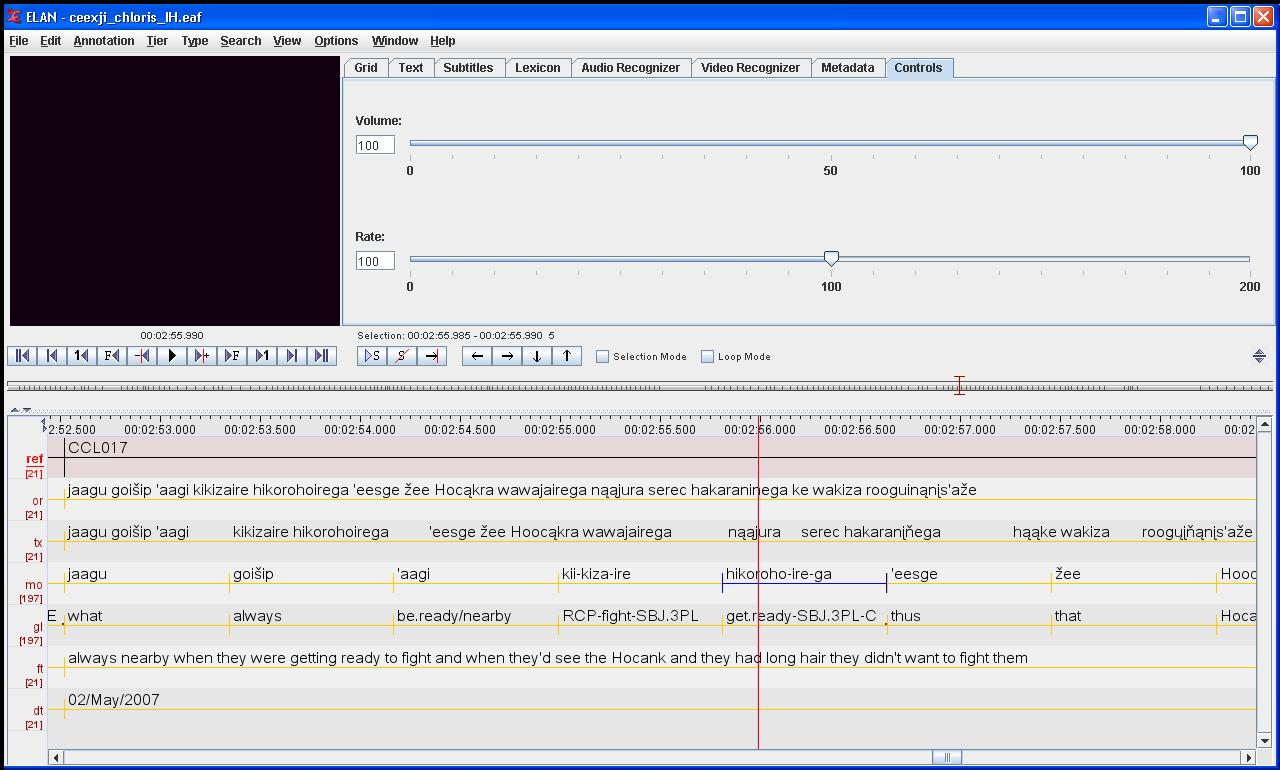
\includegraphics[width=\textwidth]{.\imgpath/Bouda-img8.jpg}
\caption{Screen shot of an annotated Hoc{\A}k (Siouan) sentence in Elan}
\label{bouda:fig:corpussentence}
\end{figure}



The tx tier contains the usually time-aligned transcription of the audio/video recording. These transcriptions are usually not based on the IPA, but on an already existing conventional orthography, or on a practical orthography developed by the documentation team. Associated with the tx tier there is a ft tier which contains the free or idiomatic translation of the target language text. The language used for the free translation is usually one of the major European languages often the one that replaces the endangered language in the community. In the example in Figure  \ref{bouda:fig:corpussentence}, this is English. Many documentation teams enriched the transcription in the tx tier and its translation in the ft tier with a second type of translation called lexical and grammatical morpheme-by-morpheme glossing. For this, a morpheme segmentation in the mo tier is matched with a gl tier that contains the lexical or grammatical glosses; cf. Figure  \ref{bouda:fig:corpussentence}.

It has to be kept in mind that these four essential parts of an annotated text involve previous and preliminary decisions on the side of the linguist that may turn out to be wrong later on in the process of the advancing documentation.

\ea
 With regard to the text tier (tx):
 \begin{enumerate}
 \item The practical orthography developed by the documentation team may be based on a wrong phonological analysis;

 \item The segmentation of the text in sentence/ utterance units may turn out to be wrong later on;

 \item The segmentation of the text into words may turn out to be wrong later on;

 \end{enumerate}
\z

\ea
 With regard to the translation tier (ft):
 \begin{enumerate}
 \item The free translation into the European language may be semantically incomplete (i.e. certain forms of the target language are not translated and are left to inference) or may contain semantic elements that are only implied in the text of the target language but are obligatory in the mediating language; 
 \end{enumerate}
\z

\ea
 With regard to the morpheme and gloss tiers (mo/gl):
 \begin{enumerate}
 \item The identification of the grammatical and lexical morphemes and their status may turn out to be wrong later on;
 \item Or, the assignment of grammatical function/ lexical meaning to a lexical or grammatical form may be wrong or incomplete;
 \end{enumerate}
\z

The main goal of the documentation of an endangered language is not the grammatical analysis of the language \textit{per se}, but the collection and processing of a representative corpus of texts in a way that a non-speaker can access it. It is hence obvious that the list of grammatical forms and lexical items has to be preliminary in the documentation process itself. However, even if there are mistakes in the transcriptions, in the translations, and in the morpheme-by-morpheme glossing, all three elements of the annotation represent an invaluable source of additional information that can be exploited in corpus linguistic searches. DOBES corpora are parallel corpora relating a morpheme-by-morpheme translation as well as a free translation to the text of the target language. This kind of additional information presupposes a preliminary phonological analysis (with regard to the transcription) as well as a preliminary grammatical analysis (with regard to the glossing). It will be shown in a moment that digital corpora of this DOBES type allow types of searches that are interesting for descriptive purposes and that go beyond the possibilities of traditional monolingual corpora. These additional search possibilities will be systematically explored in the following section.

\section{A typology of corpus linguistic searches in DOBES corpora}
% \label{bkm:Ref296525673}\label{bkm:Ref283033343}
\label{bouda:sec:typologyofsearches}

From a technical point of view the search types a descriptive linguist would like to apply to a DOBES corpus are independent of the distinction between the two basic approaches to grammar mentioned above. The most important search types are summarized in Search for a single lexical or grammatical form F1 or a single construction C1 consisting of more than one element in a single tier x1 within a linguistic context defined by the level of syntagmatic complexity/ grammatical level: and Search for the co-occurrence of two or more lexical or grammatical forms F1 and F2, or of construction C1 and C2 in one specific tier x1 or across different tiers x1-n within a linguistic context defined by the level of syntagmatic complexity/ grammatical level:.

\ea
 \begin{itemize}
\item \label{bkm:Ref283731549}Search for a single lexical or grammatical form F\tief{1} or a single construction C\tief{1} consisting of more than one element in a single tier x\tief{1} within a linguistic context defined by the level of syntagmatic complexity/ grammatical level:

 \begin{enumerate}
 \item[a)] tier x\tief{1} [...F\tief{1}...]\tief{word} [...C\tief{1}{}-C\tief{1}...]\tief{word}

 \item[b)] tier x\tief{1} [...F\tief{1}...]\tief{phrase} [...C\tief{1}{}-C\tief{1}...]\tief{phrase}

 \item[c)] tier x\tief{1} [...F\tief{1}...]\tief{clause/sentence} [...C\tief{1}{}-C\tief{1}...]\tief{clause/sentence}

 \end{enumerate}
\end{itemize}
Comments:

\begin{itemize}
\item Forms or constructions may be searched within all kinds of tiers, i.e. tier x\tief{1} = \{tx, mo, gl, ft, ...\}

\item F\tief{1} stands for a string of characters that does not exceed the word boundary, e.g. a submorpheme, a morpheme, a word, a lexical or grammatical gloss, a word of the language of translation, etc.\}

\item C\tief{1} stands for any discontinuous chain of linguistic units with a conventionalized meaning within a certain level of syntagmatic complexity, for instance circumfixes on the word level, or analytic constructions such as the \textit{will} + Verb\tief{\textsc{in}F} future construction in English;
\end{itemize}

The Search results should be presented in an interlinear version. It should be possible to store the search results/ hits as a separate data set which may be the basis for another search. It should be possible that the context size of the concordances can be determined with respect to the different levels of syntagmatic complexity (see below Table \ref{bouda:tab:gramunits}).
\z

% \ea 
Search for the co-occurrence of two or more lexical or grammatical forms F\tief{1} and F\tief{2}, or of construction C\tief{1} and C\tief{2} in one specific tier x\tief{1} or across different tiers x\tief{1-n} within a linguistic context defined by the level of syntagmatic complexity/ grammatical level:
 \begin{enumerate}
 \item[a)] tier x\tief{1} [...F\tief{1}/C\tief{1}{}-C\tief{1}...F\tief{2}/C\tief{2}{}-C\tief{2}...]\tief{word/ phrase/ clause/ sentence}

 Between the linguistic items (i.e. forms/ constructions) F\tief{1-2}/C\tief{1-2} which are searched for in this search type -- on a single tier x\tief{1} - a logical operation can be defined such F\tief{1} \{AND, OR, AND NOT etc.\} F\tief{2}, or F\tief{1} \{AND, OR, AND NOT etc.\} C\tief{1}{}-C\tief{1}, and so forth.

 \item[b)] tier x\tief{1} [...F\tief{1}/C\tief{1}{}-C\tief{1}...]\tief{ word/ phrase/ clause/ sentence} and tier x\tief{2} [...F\tief{2}/C\tief{2}{}-C\tief{2}...]\tief{ word/ phrase/ clause/ sentence}

 Between the linguistic items F\tief{1 }in tier x\tief{1} and F\tief{2} in tier x\tief{2} or C\tief{1} in tier x\tief{1} and C\tief{2} in tier x\tief{2}, and so forth, which are searched for in this search type, a logical operation can be defined such that F\tief{1} in tier \tief{1} \{AND, OR, AND NOT etc.\} F\tief{2} in tier x\tief{2}, or C\tief{1}{}-C\tief{1} in tier x\tief{1} \{AND, OR, AND NOT etc.\} C\tief{2}{}-C\tief{2} in tier x\tief{2}, and so forth.

 \end{enumerate}
% \z 


The principle types of corpus linguistic searches summarized in an abstract form in Search for a single lexical or grammatical form F1 or a single construction C1 consisting of more than one element in a single tier x1 within a linguistic context defined by the level of syntagmatic complexity/ grammatical level:{}-Search for the co-occurrence of two or more lexical or grammatical forms F1 and F2, or of construction C1 and C2 in one specific tier x1 or across different tiers x1-n within a linguistic context defined by the level of syntagmatic complexity/ grammatical level: will be applied to specific data needs of the two complementary approaches to grammar in the subsequent sections (cf. Sections\ \ref{bouda:sec:structuralgrammar} and \ref{bouda:sec:functionalgrammar}). Different questions in a semasiological approach and an onomasiological approach will be posed and it will be show how these different questions could be translated into different kinds of searches. The illustrating examples come from the Hoc{\A}k corpus \citep{HartmannEtAl2009hocank}, a DOBES corpus compiled within the DOBES project ``Documentation of the Hoc{\A}k Language'' some years ago.\footnote{Cf. 
 the website of the DOBES project ``Documentation of the Hoc{\A}k Language'' \url{http://www2.uni-erfurt.de/sprachwissenschaft/Vgl_SW/Hocank/index_frames.html} 
} 

\section{Structural grammar -- the semasiological approach}
\label{bkm:Ref283033396}
\label{bouda:sec:structuralgrammar}

The goal of a structural grammar is to identify the lexical and grammatical units (including grammatical constructions), and to find out the syntagmatic possibilities of the combinations of these units on all syntagmatic levels of complexity. There are at least four such levels of complexity: the word, the phrase, the clause (or simple sentence), and the complex sentence, cf. Table  \ref{bouda:tab:gramunits}.

\begin{table}
\begin{tabular}{p{6cm}p{6cm}}
 \textbf{grammatical units} & \textbf{levels of syntagmatic complexity}\\\hline
 submorpheme & word\\\hline
 lexical and grammatical morphemes (stems and affixes) and their combinatory possibilities & word\\\hline
 lexical and grammatical words and their combinatory possibilities & phrase\\\hline
 phrase & clause\\\hline 
 clause & (complex) sentence\\\hline
 sentence & text/ discourse\\
\end{tabular}
\caption{Grammatical units and the levels of complexity}
\label{bouda:tab:gramunits}
\end{table} 

On the word level, the descriptive linguist has to identify all lexical and grammatical morphemes of a language, their respective paradigms, and all rules of syntagmatic combinations of bound morphemes with lexical morphemes. This task implies among other things that word forms -- the primary empirical basis of this task -- have to be compared in order to find stem and affixes. This task is easier to solve if there is a preliminary analysis available in form of a morpheme-by-morpheme glossing. 

On the phrase level, the descriptive linguist has to identify all lexical and grammatical words and their possible combinations in phrases. This task is easier to solve if there is a parts-of-speech annotation which, unfortunately, is lacking systematically in DOBES corpora. 

And last but not least, on the level of the clause and complex sentence, the descriptive linguist has to determine all phrase types and their possible combinations in clauses and complex sentences. This task would be easier to solve, if there were a phrase structure annotation which is lacking in DOBES corpora as well. 

One may say that the better or richer the annotations the easier are the problems of a structural grammar to solve. Whether a text corpus comprises a morpheme-by-morpheme glossing or not makes a big difference with regard to the formulation of searches in the text corpus and the exactness and relevance of the hits one gets out of these searches. The subsequent sections illustrate some corpus linguistic methods that can be applied to DOBES corpora in order to gain data that are relevant for a structural grammar and the semasiological approach to grammar. These illustrations remain on the word level. On the higher levels of syntagmatic complexity the lack of a parts of speech and phrase structure annotation in DOBES corpora complicates the application of corpus linguistic methods. The descriptive linguist has to find indirect searches in order to identify the syntactic units a language ahs above the word level.

\subsection{Identification of lexical units}\label{bouda:sec:identificationoflexicaluntis}

Words - word forms to be more precise - can be identified in the transcription line (tx tier) by blanks at the left and the right edge. However, problematic cases arise for instance with clitics and compounds. The transcription team necessarily decided at some point in the documentation that a certain form is a clitic, or not, by using blanks. The problem is that this decision may be wrong or inconsistent throughout the corpus for various reasons (e.g. progress or changes in grammatical analysis during the transcription process, inconsistent analysis on the basis of different criteria, native speakers changing intuition etc.). Furthermore, the decision whether a combination of nouns is a coordination of phrases or a nominal compound may be difficult to draw, if there are no morphological markers that indicate this kind of relation; therefore the transcription may be inconsistent with regard to this question too. 

The identification of lexical units requires that all forms of a lexeme (including stem allomorphs) and the lexeme itself are identified together with its conventional meaning (polysemy included). Homophonous forms should be found also. There are two possibilities with regard to a DOBES corpus, either the corpus has a morpheme-by-morpheme segmentation/glossing (cf. next subsection Section\ \ref{bouda:sec:identificationoflexicaluntiswomorpheme}), or not (cf. Section\ \ref{bouda:sec:morphmebymorphemeglossing}). 

\subsubsection{Identification of lexical units: without morpheme segmentation and glossing in the corpus}
\label{bouda:sec:identificationoflexicaluntiswomorpheme}

There are three possible strategies in order to identify lexical stems: 

a) One may export all words of the target language (defined by blanks in the text corpus) and list them alphabetically. Words of the same form are simply counted; the stems of inflected or derived word forms can be found by comparison: the larger stem parts of the words are identical or at least similar. See Table  \ref{bouda:tab:hocankwordlist} for an example of this procedure from the Hoc{\A}k corpus. 

\begin{table} 
\begin{multicols}{3}
\textbf{x{\U}n{\U}}{\II}g 2

\textbf{x{\U}n{\U}}{\II}ga 1

\textbf{x{\U}n{\U}}{\II}gn{\A} 1

\textbf{x{\U}n{\k{\'u}}}{\II}gn{\A}{\A}gre 1

\textbf{x{\U}n{\U}}{\II}gn{\A}{\A}gre 2

\textbf{x{\U}n{\U}}{\II}gra 1

\textbf{x{\U}n{\U}}{\II}g\v{s}{\A}n{\A} 1

\textbf{x{\U}n{\U}}ik 1

\textbf{x{\U}n{\k{\'u}}}{\II}k 1

\textbf{x{\U}n{\U}}{\II}k 3

\textbf{X{\U}n{\k{\'u}}}{\II}ka 1

\textbf{x{\U}n{\U}}{\II}kra 2

\textbf{x{\U}{n{\k{\'u}}}{\II}kregi 1}

\textbf{x{\U}n{\U}}n{\A} 1

\textbf{x{\U}n{\k{\'u}}}n{\A}{\A}k\v{s}{\A}n{\A} 1

\textbf{x{\U}n{\U}}n{\II}{\II}sge 1

\textbf{x{\U}n{\U}}n\k{\'{i}}k 1

\textbf{xun{\U}}xj\k{\'{i}} 1

\textbf{x{\U}n{\U}}xj{\II} 1

\textbf{x{\U}n{\k{\'u}}}xj{\II}n{\II}k 1

{Xurucre 2}

{xusgajan{\A} 1}

{xuu 3}

{x{\U}{\U}n{\U} 3}

{x{\U}{\U}n{\U}{\II}g 1}

{x{\U}{\U}n{\U}{\II}gi\v{z}{\A} 1}

{x{\U}{\U}n{\U}{\II}gn{\A}{\A}ka 2}

{x{\U}{\U}n{\k{\'u}}{\II}gn{\A}ka 1}

{x{\U}{\U}n{\U}{\II}gra 1}

{x{\U}{\U}n{\U}{\II}k 3}

{x{\U}{\U}n{\U}{\II}kra 1}

{x{\U}{\U}n{\U}n\k{\v{a}} 5}

{x{\U}{\U}n{\U}n{\A}ka 1}

{X{\U}{\U}n{\U}n{\II}kga 1}

{x{\U}{\U}n{\k{\'u}}n{\II}kjeega 1}

{x{\U}{\U}n{\U}n{\II}kra 1}

{x{\U}{\U}n{\U}xj\k{\'{i}} 1}

{x{\U}{\U}nuxj{\II}gra\v{s}ge 1}

{x{\k{\'u}}{\U}n{\U}xj{\II}n{\II}kra 1}

{x{\U}{\U}n{\U}\v{z}e 1} 
\end{multicols} 
\caption{Extract from the word list of the entire Hoc{\A}k corpus: \textit{x{\U}n{\U}}  `small, little'}
\label{bouda:tab:hocankwordlist}
\end{table}


Table \ref{bouda:tab:hocankwordlist} contains a segment of all word forms of the Hoc{\A}k corpus alphabetically sorted. This wordlist was compiled and exported with Elan. The segment in Table \ref{bouda:tab:hocankwordlist} contains all word forms that resemble the lexeme \transcr{x{\U}n{\U}}{small, little} in the corpus. As can be seen in this list, there are derived forms of \transcr{x{\U}n{\U}}{small, little} with different suffixes, and there are compounds of \transcr{x{\U}n{\U}}{small, little} with other lexemes. In addition, it is obvious that there are inconsistent spellings of \transcr{x{\U}n{\U}}{small, little}, the forms in bold with short vowels, the forms in the last two columns with a long stem vowel. Nevertheless, this method allows identifying stems by means of comparison of the similar word forms and, in addition, it is possible to some degree to identify the allomorphs of the lexical morpheme. A problem arises with prefixed word forms. They appear in another segment of the alphabetical list of words, but see Figure \ref{bouda:fig:concordances} below. The list in Table \ref{bouda:tab:hocankwordlist} exhibits also a minor technical problem with Elan, the annotation software with which the word list was generated. Elan ignores the nasal /\textit{{\U}}/ vs non-nasal /u/ in the sort order, so that different words appear in the middle of the list (e.g. \transcr{xuu}{leg}), it also ignores stressed vowels which is, however, helpful in this case.

b) The second strategy may be to search for strings which are hypothetically part of the word stems in the object language (using regular expressions, if necessary); for instance, if you search for \textit{x{\U}n{\U}} 'small' in the tx tier of the corpus, you'll get 37 hits, among them also forms with prefixes as can be seen in the concordances in Figure \ref{bouda:fig:concordances} below. The advantage of this strategy is that you get prefixed and suffixes as well as compounded forms of the hypothetical stem. The disadvantage, however, is that spelling alternations and stem allomorphy is ignored.
% 
% \begin{table} 
% \begin{tabular}{p{5cm}lp{5cm}}
% ``{s'iireja} &
% {h\k{i{x{\U}n{\U}}{\II}gregi}} &
% {hi'{\U}n{\II} haara taan{\II}\v{z}u n{\A}{\A} 'eeja ruus\v{s}{\U}n{\U}regi hagijite\v{s}{\U}n{\U}}''\\\hline
%  &
% {``h\k{i{x{\U}n{\U}}\v{n}eegi}} &
% {heg{\U} haahe teegi \v{z}oo\v{z}ocra roigixrawii\v{s}un{\U}.}''\\\hline
%  &
% {``h\k{i{x{\U}n{\U}}{\II}gregi\v{s}ge}} &
% {hicooke haara\v{s}ge wa\v{z}{\A}n{\A} rooh{\A}xj{\II} h{\U}{\U}kirakra waak{\II}k{\U}n{\U}n{\II} waa'{\U}n{\A}k\v{s}{\A}n{\A}}''\\\hline
%  {``h{\A}h{\A}; x'ookera} &
% \textbf{{x{\U}n{\U}}{\II}gn{\A}{\A}gre} &
% {jaasge wagigires'agi tee tee hi\v{z}{\A} hi\v{z}{\A} wagan{\A}{\A}gre}''\\\hline
%  {``h{\A}h{\A}, jaasge} &
% {h\k{i{x{\U}n{\U}}{\II}gjeegi\v{s}{\A}n{\A}}} &
% {hahi woto\v{g}ocn{\II}sge\v{s}{\U}n{\U}}''\\\hline
%  {``horu\v{s}j{\A} hi\v{z}{\A} heg{\U} tee heg{\U} tee heg{\U} hagorei\v{z}{\A} Heen{\A}ga tee hi\v{z}{\A} Heen{\A}} &
% \textbf{{x{\U}n{\U}}n{\A}} &
% {Emmanuelga horujisra (hi??)\v{z}{\A} hagorei\v{z}{\A} heg{\U}}''\\\hline
%  {``hija 'an{\A}ga heg{\U}...} &
% {wa\v{z}{\A}su}\textbf{{x{\U}n{\U}}{\II}g} &
% {n{\II}{\II}sge jagu\v{s}ge wigairera?}''\\\hline
%  {``heg{\U}} &
% \textbf{{x{\U}n{\U}}{\II}g\v{s}{\A}n{\A}''} &
% \\\hline
%  {``gota\v{s}ge wa\v{z}{\A} hee wigan{\A}k 'eegi ceerap} &
% {h{\II}x{\U}n{\U}wiregi} &
% {ceerap wiagawi\v{s}{\U}n{\U}}''\\\hline
%  {``N{\II}kuse} &
% {(Ho)}\textbf{{x{\U}n{\U}}\v{n}{\A}} &
% {\v{z}e'e\v{s}ge that's the Wisconsin River \v{z}ee ho'{\U}{\II}\v{n}ekjanen{\A} N{\II}oxawan{\II}ra\v{s}ge ho'{\U} hikiware hikiwarairekjanera \v{z}ee 'eeja '{\U}{\II}\v{n}ekjanen{\A}}''\\\hline
%  {``P{\II}hi wes\k{\'{i}}w{\II}-gaj{\A} tew\'oiraki n{\II}\v{s}\'an{\A}k} &
% \textbf{{x{\U}n{\k{\'u}}}xj{\II}n{\II}k} &
% {.-h\'i\v{z}{\A}; hat'{\A}pji-\'an{\A}ga wa'{\U}j\'e\v{z}e.''}
% 
% \end{tabular}
% \caption{Selected concordances of a search of \textit{x{\U}n{\U}} `small'}
% \label{bouda:tab:concordances}
% \end{table} 

\begin{figure}
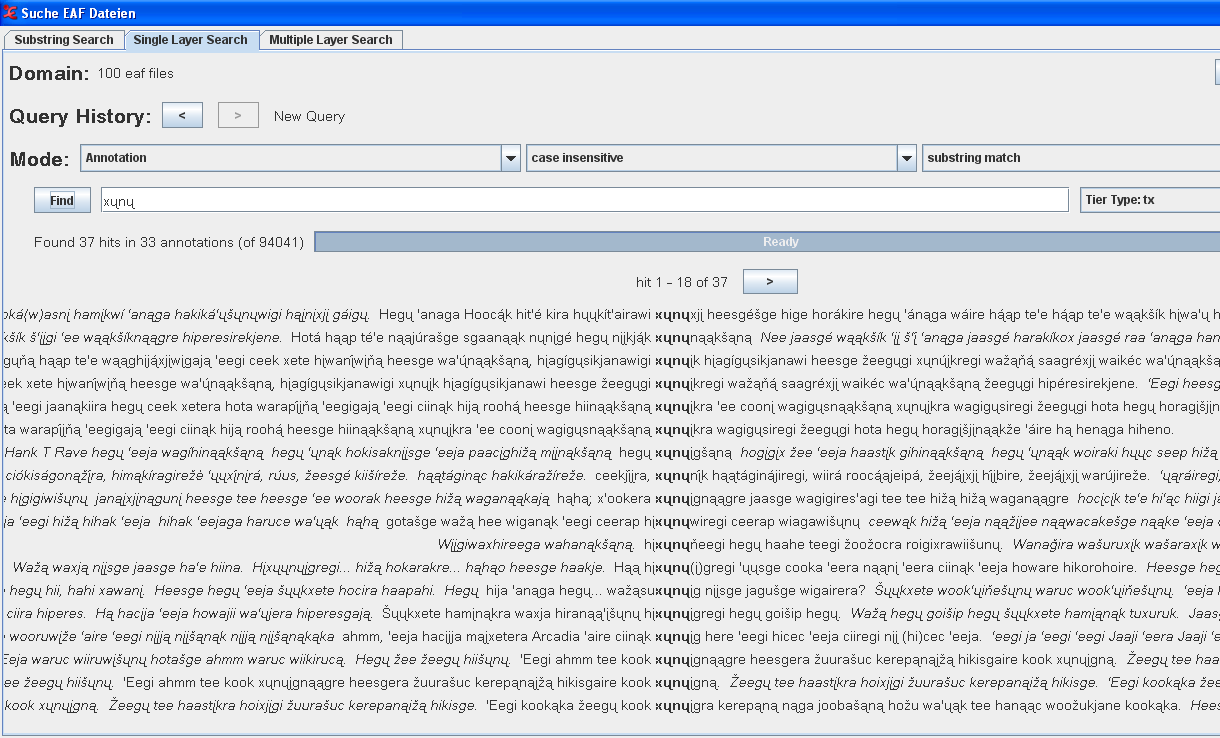
\includegraphics[width=\textwidth]{.\imgpath/BoudaKonkordanz.png}
\caption{Selected concordances of a search of \textit{x{\U}n{\U}} `small'}
\label{bouda:fig:concordances}
\end{figure}

c) The third strategy starts from the translation tier. One may search for a lexical item in the free translation ft tier assuming that there is a lexical match in the object language. For instance, if you search for \textit{small/little} in the ft tier, you indeed get lexical matches in the target language, cf. \xref{bouda:ex:ED3024}, or you get forms with a diminutive marker (glossed DIM) as can be seen in \xref{bouda:ex:CTD003}. 

\newpage
\let\eachwordthree=\rm
\ea\label{bouda:ex:ED3024}
ref ED3024
\glll 
tx cii x{\U}{\U}n{\U}{\II}k hi\v{z}{\A} '{\U}{\U}    \\
mo cii x{\U}{\U}n{\U}-{\II}k hi\v{z}{\A} '{\U}{\U}     \\
gl house be.small(\textsc{obj}.\textsc{3sg})-\textsc{dim} one do/make(\textsc{sbj}.\textsc{3sg})      \\\

\glll 
tx jaagu n{\II}{\II} hicec 'eeja \\
mo jaagu n{\II}{\II} hicec \\
gl  what water near\\

ft he made a small house by the river\\
dt 25/Oct/2004\\
\z
 
\ea\label{bouda:ex:CTD003}
ref CTD003
\glll 
tx \v{z}ee ceek hon{\U}w{\A}k 'eeja tee hoc{\II}c{\II}gi\v{z}{\A}, n{\II}{\II}kj{\A}k n{\A}{\A}gre \\
mo \v{z}ee ceek ho-n{\U}w{\A}k 'eeja tee hoc{\II}c{\II}-{\II}g-i\v{z}{\A} n{\II}{\II}kj{\A}k n{\A}{\A}gre\\
gl that first/new \textsc{appl}.\textsc{iness}-run there this \textbf{boy-\textsc{dim}-one} child these\\
ft from the start, \textbf{a little boy}, these children...ahm... \\
dt 11/May/2006\\
\z

In \xref{bouda:ex:ED3024}, the result of the search is the expected property word \textit{x{\U}{\U}n{\U}-{\II}k '}small-DIM', however, with the diminutive marker \textit{--(n){\II}k}; in \xref{bouda:ex:CTD003}, there is no lexical equivalent of the search item 'small', instead one gets a noun with a diminutive marker only. This strategy has the advantage to provide an overview of the forms in the target language that correspond a specific form of the language of translation. It is hence a search type that rather belongs to the onomasiological approach. In addition, it allows the identification of the allomorphs of a morpheme. Another advantage is that this strategy allows the finding of lexical paradigms and stem suppletivism. The disadvantage is that this strategy ignores the polysemy (manifest as variation in the translation) of a form.

\subsubsection{With morpheme-by-morpheme glossing in the corpus}
\label{bouda:sec:morphmebymorphemeglossing}
The identification of lexical stems is of course much easier, if there are morpheme breaks and a glossing of the lexical and grammatical morphemes. The morpheme-by-morpheme interlinear glossing presupposes an analysis of lexical and grammatical forms. The mo tier contains the underlying or standardized form of the grammatical and lexical morpheme, and the gl tier attributes the standard glossing (\textit{Grundbedeutung}) of the morpheme. Searches of the lexical item on the mo tier allow finding the allomorphs of a lexical morpheme by comparing the hits with the corresponding form on the tx tier. For instance, in the Hoc{\A}k corpus, there are quite a few variously abbreviated forms of \textit{an{\A}ga} 'and' such as \textit{-n{\A}ga} in the tx tier which could not be found otherwise. These forms are allomorphs of \textit{an{\A}ga}.

\subsection{Identification of grammatical units}

The Identification of grammatical units requires the establishment of the morpheme-allomorph pairings and its grammatical meanings or functions. With respect to corpus linguistic searches in DOBES corpora, there are two possibilities: either the corpus has a morpheme-by-morpheme segmentation/glossing, or not. 

\subsubsection{Identification of grammatical units: without morpheme segmentation and glossing in the corpus}
The methods to be applied here are quite similar to the ones applied for the identification of lexical units, see above Section\ \ref{bouda:sec:identificationoflexicaluntis}. The first strategy is to export all words of the target language (defined by blanks in the text corpus) and list them alphabetically. The inflected and derived word forms will show up in the list if the stems remain formally constant and have no prefixes. One has to look for systematic variations with regard to form-meaning pairings in the tx line and the ft line. If there are systematic form-meaning variations with respect to some affix-like form or with respect to some potential grammatical words, one can proceed with searching these forms in the text tx tier. For instance, in Hoc{\A}k, progressive aspect is systematically expressed by means of certain verb-auxiliary analytical constructions. Once the construction is discovered, one may search these constructions systematically on the tx tier.

Another strategy could start with prototypical nouns and verb, since grammatical variation can be expected to occur primarily with words of the open classes. These prototypical nouns and verbs have to be looked for in the translation ft tier. Under the assumption that for instance inflected verbs in the translation ft tier correspond to inflected verbs in the text tx tier, one may start with searches for prototypical verbs and nouns in the ft tier. This strategy can be applied also to grammatical meanings: grammatical meanings such as personal pronouns ('I', 'you', etc.), progressive aspects (e.g. 'V-\textit{ing}'), and so forth can be searched for in the translation ft tier. The results can be compared with what corresponds to it in the tx line of the object language. The problem with this kind of search is that one will not find complete paradigms in the text corpus. Elicitation of forms with a native speaker is much more promising here as a strategy.

The latter strategy can be exemplified with an example from the Hoc{\A}k corpus. If one want to find out, if progressive aspect (PROG) is marked grammatically in Hoc{\A}k, one may search for \textit{V-ing} constructions in the translation ft tier. Of course, the range of hits one gets is much wider than just the clear progressive uses of this form, since the \textit{--ing} form in English is not restricted to progressive aspect. So, one has to select from the results of this search the cases which seem to be good cases of a progressive meaning in English and may compare this with the forms in the text tx tier.

A variation of this kind of search is to choose a specific probably frequent verb and search for its progressive construction in the translation tier. For example, a search for ``was looking'' receives 6 hits in the Hoc{\A}k corpus with quite interesting results. First of all, one gets the standard analytic construction in Hoc{\A}k for the expression of progressive aspect (cf. the text in bold in the second line of example \xref{bouda:ex:TWI026} corresponding to the English meaning 'listening to them'); it is one possible verb auxiliary construction for progressive aspect; but one gets also an alternative expressions such as the reduplication (cf. first line in example \xref{bouda:ex:TWI026} which corresponds to 'was looking'), and more astonishing, a construction with the habitual marker (glossed \textsc{hab}) on the verb, cf. \xref{bouda:ex:HOR029}. 


\ea\label{bouda:ex:TWI026}
ref TWI026
\glll 
tx Heg{\U} heg{\U} han\'{\A}{\A}c horo\v{g}\'o\v{g}oc heg{\U}          \\
mo heg{\U} heg{\U} han{\A}{\A}c     horo$<$\v{g}o$>$\v{g}oc heg{\U}         \\
gl that.way that.way all \textbf{$<$\textsc{rdp}:\textsc{iter}$>$look.at(\textsc{sbj}.\textsc{3sg})} that.way     \\
\glll
tx wan\'{\A}xg{\U} wa'{\U}{\A}k\v{s}{\A}n{\A} heg{\U} {} \\ 
mo wa-n{\A}{\A}xg{\U} wa'{\U}-'{\A}k-\v{s}{\A}n{\A} heg{\U} \\
gl \textbf{\textsc{obj}.\textsc{3pl}-hear(\textsc{sbj}.\textsc{3sg})} \textbf{do/be-\textsc{pos}.\textsc{hor}-\textsc{decl}} that.way\\

ft It was looking all around and listening to them.\\
dt 21/Sep/2006\\
\z
 
\ea\label{bouda:ex:HOR029}
ref HOR029
\glll 
tx Hoto\v{g}ocnaga heg{\U} \v{s}{\II}{\II}cra\v{s}ge n{\A}{\A}sura...     hoip{\II}n{\II} \\
mo hoto\v{g}oc-n{\A}ga heg{\U} \v{s}{\II}{\II}c-ra-\v{s}ge n{\A}{\A}su-ra hoip{\II}n{\II}   \\
gl look.at{\textbackslash}\textsc{1e.a}-and that.way rear-\textsc{def}-also head-\textsc{def}        spin                \\
\glll
tx haakirin{\A}k heg{\U}        hakjopahi\v{s}ge              \\
mo ha$<$ha$>$kirin{\A}k heg{\U} hakja-ho-hapahi-\v{s}ge         \\
gl $<$1\textsc{e.a}$>$land.on that.way   back-\textsc{appl}.\textsc{iness}-go.toward-also    \\
\glll
tx ham{\II}{\A}n{\A}kn{\A}ga\v{s}ge, c{\A}{\A}geja g{\U}{\A}gaira horo\v{g}ocn{\II}{\II}sge\v{s}{\U}n{\U}.\\
mo ham{\II}$<$ha$>$n{\A}k-n{\A}ga-\v{s}ge c{\A}{\A}k-'eeja g{\U}{\A}gaira horo\v{g}oc-n{\II}{\II}sge-\v{s}{\U}n{\U} \\
gl  $<$1\textsc{e.a}$>$sit.on-and-also outside-there sometimes look.at-\textsc{vague}-\textsc{hab}\\

ft I got on it and spun around on it \textbf{glancing} outside once and a while, while I \textbf{was looking} over the back end.\\
dt 22/Sep/2006\\
\z



Especially the latter result is due to the polysemy of the English progressive aspect on \textit{--ing} which obviously can be used to express habitual meanings too. The latter type of search equally belongs to the onomasiological approach to grammar.

\subsubsection{With a morpheme-by-morpheme segmentation and glossing in the corpus}
If grammatical morphemes are already glossed, it is of course easy to find all its allomorphs and all its meanings. Just look for the grammatical gloss on the gloss tier. For instance, if one looks for the Hoc{\A}k future tense marker glossed \textsc{fut} one finds at least five different forms (allomorphs) for this marker --\textit{kjene} '\textsc{fut}', cf. Table \ref{bouda:tab:future}. 

\begin{table}
\begin{tabular}{lll}
 \textbf{allomorphs} &
 \textbf{grammatical meanings/functions} &
 \textbf{gloss}\\\hline
\parbox{2cm}{
  \textit{-kje }\\
  \textit{-kjane}\\
  \textit{-kjene}\\
  \textit{-kj{\A}n{\A}he}\\
  \textit{-kjenehe}
} 
&
future intentional, irrealis, desiderative, obligation &
\textsc{fut}\\
\end{tabular}
\caption{Allomorphs of the future tense marker \textit{--kjene} \textsc{fut} in the Hoc{\A}k corpus}
\label{bouda:tab:future}
\end{table}

The results of this search show that there is some allomorphy associated with this morpheme and, in addition, that this morpheme is actually polyfunctional. It marks future tense, but also different kinds of modal meanings such as 'should' and others.

\newpage
\subsection{Word internal morphological structure -- the combination of lexical and grammatical morphemes}
\label{bouda:sec:wordinternalmorphologicalstructure}

The task here is to find out the possible combinations of lexical and grammatical morphemes within the word; in case that clitics are involved the searches have to transcend the word boundary. This can be done in a DOBES corpus with an interlinear glossing simply by searching the grammatical item and analyzing the forms that appear to the left or to the right in the concordances. This search can be executed on the morpheme break mo tier or on the gloss gl tier. This kind of search can be illustrated with an example from Hoc{\A}k. 

Hoc{\A}k verbs have quite complex chains of suffixes and enclitics which are all formally identified. However, the possible syntagmatic combinations are not known. In order to find this out, all kinds of combinations of grammatical suffixes/ enclitics [stem-X- ....-Y] with all kinds of morphemes in between have to be searched. Because of the morpheme glossing in this corpus, it is easy to find all syntagmatic combinations of the relevant grammatical formatives. It suffices to search for the gloss and then analyze the chains of suffixes/ enclitics. For instance, if one searches for the gloss \textsc{fut} which is the gloss for the future tense marker --\textit{kjene} '\textsc{fut}' and its allomorphs, one gets chains of glosses like the ones given in Figure  \ref{bouda:fig:futuresearch}. As can be seen already from this selection, the variety of grammatical formatives that may follow the \textsc{fut} marker or that precede it is remarkable. In order to arrive at a kind of morphological template for the suffixes/ enclitics in Hoc{\A}k verbs, various combinations have to be searched for.

% \begin{table} 
% \begin{multicols}{2}
% ``1PI.A-\textsc{obj}.3\textsc{pl}-use-\textsc{neg}.\textsc{fin}-\textbf{\textsc{fut}}{}-\textsc{pl}-\textsc{def}]''
% 
% ``\textsc{obj}.3\textsc{pl}-$<$1\textsc{e.a}$>$use-\textsc{neg}.\textsc{fin}-\textbf{\textsc{fut}}{}-\textsc{def}]''
% 
% ``1PI.A-$<$RFL$>$tear.out-0-\textbf{\textsc{fut}}{}-\textsc{pl}]''
% 
% ``1PI.A-go.there-\textbf{\textsc{fut}}{}-\textsc{pl}-\textsc{def}]''
% 
% ``[1PI.U-AP\textsc{pl}.BEN-be.lost-\textsc{neg}.\textsc{fin}-\textbf{\textsc{fut}}{}-\textsc{pl}-\textsc{def}]]''
% 
% ``1PI.A-pick.up-\textbf{\textsc{fut}}{}-\textsc{pl}''
% 
% ``1PI.A-make/\textsc{caus}-\textsc{neg}.\textsc{fin}-\textbf{\textsc{fut}}{}-\textsc{pl}]''
% 
% ``1PI.A-attempt-\textbf{\textsc{fut}}{}-\textsc{pl}''
% 
% ``$<$1\textsc{e.u}$>$catch.up.to-\textsc{sbj}.3\textsc{pl}-\textsc{pl}-\textsc{neg}.\textsc{fin}-\textbf{\textsc{fut}}{}-\textsc{caus}AL''
% 
% ``go.forward-\textsc{sbj}.3\textsc{pl}-\textbf{\textsc{fut}}{}-\textsc{top}''
% 
% ``go.about-go.there-\textsc{sbj}.3\textsc{pl}-\textsc{neg}.\textsc{fin}-\textbf{\textsc{fut}}{}-\textsc{top}''
% 
% ``\textsc{obj}.3\textsc{pl}-1\textsc{e.a}-\textsc{pos}S.RFL-respect-0-\textbf{\textsc{fut}}{}-\textsc{pl}''
% 
% ``arrive.here(\textsc{sbj.3sg})-\textbf{\textsc{fut}}{}-\textsc{top}''
% 
% ``arrive.going-\textbf{\textsc{fut}}{}-\textsc{decl}''
% 
% ``\textbf{coll}-arrive.there-\textsc{sbj}.3\textsc{pl}-\textbf{\textsc{fut}}{}-\textsc{top}''
% 
% ``arrive.here(\textsc{sbj.3sg})-\textbf{\textsc{fut}}{}-\textsc{top}''
% 
% ``1\textsc{e.a}-do/make-\textbf{\textsc{fut}}{}-thus''
% 
% ``2.A-warhoop-0-\textbf{\textsc{fut}}{}-\textsc{top}''
% 
% ``2.A-warhoop-0-\textbf{\textsc{fut}}{}-\textsc{top}''
% 
% ``***-\textbf{\textsc{fut}}{}-\textsc{pl}-\textsc{top}''
% 
% ``be.funny(\textsc{obj}.3\textsc{sg})-DIM-\textbf{\textsc{fut}}{}-\textsc{neg}.\textsc{fin}''
% 
% ``\textsc{obj}.3\textsc{pl}-tell{\textbackslash}1\textsc{e.a}-0-\textbf{\textsc{fut}}{}-***''
% 
% ``$<$1\textsc{e.a}$>$say.to-\textsc{neg}.\textsc{fin}-\textbf{\textsc{fut}}{}-\textsc{pl}''
% 
% ``say{\textbackslash}1\textsc{e.a}-\textsc{neg}.\textsc{fin}-\textbf{\textsc{fut}}{}-\textsc{pl}''
% 
% ``$<$1\&2$>$see{\textbackslash}1\textsc{e.a}-\textbf{\textsc{fut}}{}-\textsc{pl}-SEQ''
% 
% ``1\textsc{e.u}-make/\textsc{caus}-\textbf{\textsc{fut}}{}-\textsc{pl}-\textsc{top}''
% 
% ``do/make-\textsc{sbj}.3\textsc{pl}-\textbf{\textsc{fut}}{}-\textsc{top}]''
% 
% ``make/\textsc{caus}{\textbackslash}1\textsc{e.a}-\textbf{\textsc{fut}}{}-\textsc{top}]''
% 
% ``that's.why-\textbf{\textsc{fut}}{}-\textsc{top}]''
% 
% ``know-\textsc{sbj}.3\textsc{pl}-\textbf{\textsc{fut}}{}-DUB]''
% 
% ``go.through(\textsc{sbj.3sg})-\textbf{\textsc{fut}}{}-\textsc{caus}AL''
% 
% ``2.A-do/make-\textbf{\textsc{fut}}{}-\textsc{pl}-\textsc{decl}''
% 
% ``\textsc{obj}.3\textsc{pl}-$<$1\textsc{e.a}-AP\textsc{pl}.BEN$>$forbid-\textbf{\textsc{fut}}{}-\textsc{decl}''
% \end{multicols}
% \caption{Selection of hits of a search for the gloss \textsc{fut} (future tense marker) in the gl tier}
% \label{bouda:tab:futuresearch}
% \end{table} 

\begin{figure}
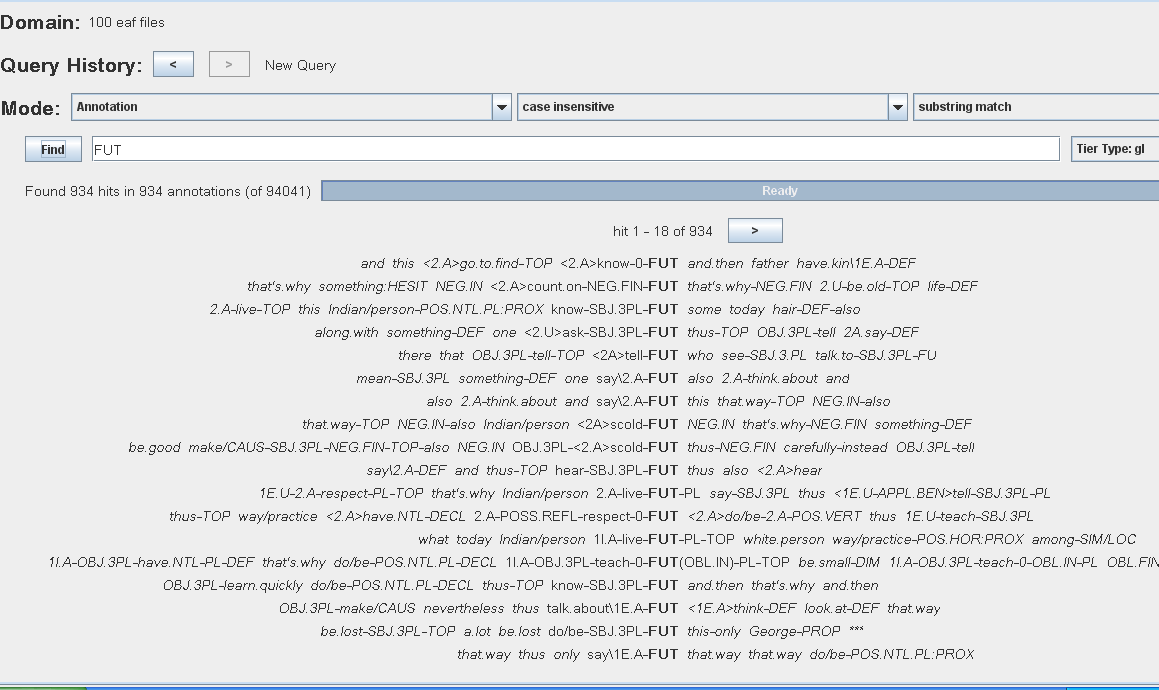
\includegraphics[width=\textwidth]{.\imgpath/BoudaSearchFUT.png}
\caption{Selection of hits of a search for the gloss \textsc{fut} (future tense marker) in the gl tier}
\label{bouda:fig:futuresearch}
\end{figure}


Another question would be: how to examine morphophonemic processes with corpus linguistic methods in DOBES corpora. Hoc{\A}k has heavy morphophonemic processes in the prefixes, i.e. the outcome of the combination of two prefixes often results in a very opaque form. See, for instance, \textit{h{\U}{\U}ro\v{g}oc} 'he was looking at me' which appears in example \ref{bouda:ex:HOR068}. The underlying form is: \textit{ho-{\II}-{\OO}-ro\v{g}oc} with a divided stem \textit{ho-ro\v{g}oc} 'look at' and the pronominal infixes 1\textsc{sg.ug}(me)-\textsc{3sg.a}(he). 
 
\ea\label{bouda:ex:HOR068}
ref HOR068
\glll 
tx Heg{\U} wogitekji        \textbf{h{\U}{\U}ro\v{g}oc}         \\
mo heg{\U} woogitek-xj{\II} \textbf{ho$<${\II}-\O-$>$ro\v{g}oc}   \\
gl that.way be.angry-\textsc{ints}   \textbf{$<$1\textsc{e.u}-\textsc{3sg.a}$>$look.at}        \\
\glll
tx wa'{\U}{\A}k\v{s}{\A}n{\A}, heg{\U} 'eeja n{\U}{\U}giw{\A}kj{\II}  \\  
mo wa'{\U}-'{\A}k-\v{s}{\A}n{\A} heg{\U} 'eeja n{\U}{\U}giw{\A}k-j{\II} \\
gl do/be(\textsc{sbj.3sg})-\textsc{pos.hor}-\textsc{decl} that.way there run-\textsc{ints}                    \\
\glll
tx kirikere haa. \\
mo kiri-kere haa \\
gl arrive.back.here-go.back.there make/\textsc{caus}{\textbackslash}1\textsc{e.a}\\

ft He was looking at me real mad and I left there running fast.\\
dt 25/Sep/2006\\
\z

What happens here is that the underlying pronominal affixes merge with the first part of the stem in quite unpredictable ways. The morphophonemic process can easily be examined by comparison of the gloss in the gl tier with the form in the text tx tier. In order to find out, whether this type of morphophonemic process happens regularly, one may search for the string \textit{h{\U}{\U}} in the text tx tier to get all instances of this process. Unfortunately, this search gives also words that are not inflected in this way such as \textit{h{\U}{\U}c} 'bear' and \textit{h{\U}{\U}k} 'chief'\textbf{\textit{.}} A solution would be to search across tiers, the form \textit{h{\U}{\U}} itself in the tx line, and the function 1\textsc{sg.ug}-\textsc{3sg.a} in the gl tier, in order to avoid to get all words that begin with \textit{h{\U}{\U}-}. 

\subsection{Beyond the word level}
\label{bouda:sec:beyondthewordlevel}

Structural units beyond the word level of complexity comprise grammatical categories that are expressed analytically, the internal structure of different phrase types such as the NP, the VP, the PP and so on, the constituent structure of the clause and the structure of complex clauses. The descriptive task of a structural grammar is to describe the internal structure and the distribution of these syntactic categories and constructions. For instance, in order to describe the NP as a syntactic category one has to find out the kinds of elements that may be combined in a NP and their possible order(s) within this constituent type. The problem for the corpus linguistic methods is that DOBES corpora do not have a syntactic annotation. Neither parts of speech nor phrases such as NPs etc. are annotated. Therefore, the descriptive linguist is forced to formulate indirect search routines in order to identify the intended phrase type, e.g. a NP. For instance, in Hoc{\A}k, most NPs end with a determiner on the right edge. Searching for these determiners (e.g. definite and indefinite articles, demonstrative pronouns) could be a way to find NPs in the text corpus. However, many subordinate clauses have a definite article on the right edge too, so they have to be filtered out by a second procedure. Another problem would arise that there are also NPs that have no determiners in this slot. Another possibility would be to search for nouns assuming that they always occur in NPs. This is not possible, since parts of speech are not annotated. In addition, there are NPs without nouns as heads. 

So, it can be concluded that the lack of a syntactic annotation hinders the corpus linguistic treatment of DOBES corpora quite a bit. It would be desirable to have a tool for the automatic or semi-automatic syntactic annotation of DOBES corpora to make them apt for the searches the descriptive linguist needs to analyze the syntax of the target language. This holds for the phrase level, the clause level and the sentence level of syntagmatic complexity.

Another question are grammatical categories that are expressed analytically. In principle, there is the possibility to search for one element of such a construction and then to compare the hits which contain the second element of such a construction with the ones in which this element does not occur. The other possibility is to look for the whole construction, i.e. a combination of two elements that belong to the construction. In the search string one has to specify the two elements by strings of characters and the number of elements that may interrupt this construction by variables (with certain regular expressions). For instance, in Hoc{\A}k, the modal meaning 'must not' is expressed by means of a combination of the future suffix \textit{-- kje} and a separate word \textit{heesg\'e} following the verb. Both elements occur independently with a specific meaning, but in combination they have the meaning 'must not' which cannot composed out of the elements. In the Hoc{\A}k corpus, this construction has already been identified and was glossed accordingly, cf. \xref{bouda:ex:ALV022}: 
 
\ea   \label{bouda:ex:ALV022}
ref ALV022
\glll 
tx Ciir\'a\v{s}ge hi\v{z}{\k{\'a}}  paag\'axwigi heg{\U} wa\v{z}{\k{\'a}}         \\    
mo cii-ra-\v{s}ge hi\v{z}{\A} paagax-wi-gi heg{\U} wa\v{z}{\A} \\ 
gl house-\textsc{def}-also one write(draw){\textbackslash}1\textsc{e.a}-\textsc{pl}-\textsc{top} that.way something  \\
\glll
tx hij{\A}h\k{\'{i}}n{\A} hi\v{z}\'{\A} paag\'axwigi m{\A}{\II}xet\'e cii          \\
mo  hij{\A}h{\II}-ra hi\v{z}{\A} paagax-wi-gi m{\A}{\II}xete cii                                          \\
gl different-\textsc{def} one write(draw){\textbackslash}1\textsc{e.a}-\textsc{pl}-\textsc{top} white.person house            \\
\glll
tx paag\'axikjawi  heesgera h{\A}{\A}k\'e heesge                                    \\           
mo \textbf{paagax-i-kje-wi} \textbf{heesge-ra} h{\A}{\A}ke heesge                     \\         
gl \textbf{write(draw){\textbackslash}1\textsc{e.a}-0-\textsc{obl}.\textsc{in}-\textsc{pl}} \textbf{\textsc{obl}.\textsc{fin}-\textsc{def}} \textsc{neg}.\textsc{in} that's.why\\ 
\glll
tx hawin{\II} 'eegi jaagu waac\'i          \\                                 
mo haa-wi-n{\II} 'eegi jaagu wa-ha-cii       \\                               
gl make/\textsc{caus}{\textbackslash}1\textsc{e.a}-\textsc{pl}-\textsc{neg}.\textsc{fin} and.then what \textsc{obj}.3\textsc{pl}-1\textsc{e.a}-live \\
\glll
tx han{\A}kwigi heesge paag\'axwigi      \\                                   
mo ha-n{\A}k-wi-gi heesge paagax-wi-gi     \\                                 
gl 1\textsc{e.a}-\textsc{pos}.\textsc{ntl}.\textsc{pl}-\textsc{pl}-\textsc{top} that's.why write(draw){\textbackslash}1\textsc{e.a}-\textsc{pl}-\textsc{top} \\
\glll
tx woogit\'ekire.\\
mo woogitek-ire \\
gl get.angry/mad-\textsc{sbj}.3\textsc{pl}\\
ft When we drew a house, \textbf{we were supposed to draw the white man's house}, if we drew what we were living in or something different they would get mad.\\
dt 23/Jul/2007\\
\z

However, if this is not the case, one has to formulate a complex search or to formulate subsequent searches in order to identify constructions like these. 

\section{Functional grammar -- the onomasiological approach}
% \label{bkm:Ref283033425}
\label{bouda:sec:functionalgrammar}

The goal of the onomasiological approach to grammar is to describe in a systematic way the linguistic means by which in the target language a certain general function can be expressed. This approach to grammar requires searching for semantic functions/ concepts and operations that are considered to be necessary more or less for each language. They are therefore considered universal. It is self-evident that there cannot be a complete list of such functions. Table \ref{bouda:tab:functionaldomains} presents a summary of the most important (probably universal) tasks a language has to be able to fulfill. 
 

\begin{table} 
\footnotesize
\begin{tabular}{p{2cm}p{3cm}p{3cm}p{3cm}}
\textbf{domain} &
\textbf{basic functions} &
\textbf{representative concepts and operations} &
\textbf{lexical expressions and grammatical constructions in English as cues for certain semantic concepts}\\\hline
apprehension \&

nomination &
an entity is grasped by categorizing and individuating it; it is named by a label or a descriptive expression &
categorization, types of concepts, empathy &
\textsc{num}-\textsc{n}

\textsc{n}-\textsc{sg}/\textsc{pl}\\\hline
concept modification &
a concept is enriched, or an object is identified &
attribution, apposition, relativization &
\textsc{adj-n}, \textsc{ptc-n}, \textsc{n-rel} constructions, \textsc{pro/prop}-appositions\\\hline
reference &
a representation is related to and delimited within the universe of discourse &
determination, deixis, reference tracking &
\textsc{dem-n}, 

\textsc{def-n}, \textsc{in}\textsc{def-n}, 

\textsc{sap-pro},

Non-\textsc{sap} 3\textsuperscript{rd} person pronouns \\\hline
possession &
the relation of an entity to another one is established or inheres in one of them &
possession in reference, possessive predication, external possessors &
genitive attribute (-\textit{s/ of})

verbs of possession (\textit{have, belong})

dative of possession (e.g. \textit{carry sth. for so.})\\\hline
spatial orientation &
an entity is localized in space statically or dynamically &
reference points, local relations, spatial and gestalt properties of objects &
spatial adverbs

\textsc{n}\tief{1} \textsc{prep-n}\tief{2} constructions with \textsc{n}\tief{1} as the Figure (object localized) and N\tief{2} as the Ground (region/ frame of reference)\\\hline
quantification &
the extent of the involvement of a set of entities in a predication is delimited &
quantification in reference and in predication; counting, ordering &
\textsc{n}-\textsc{sg}/\textsc{pl}

\textsc{num/quant-n}

numeral adverbials 

cardinal and ordinal numbers\\\hline
predication &
information is attributed to a referent &
existence, situation, characterization &
X is Y

X is a Y/ Xs are Ys

there is a X

X is \textsc{prep} \textsc{np}

X is \textsc{poss.pro} Y

and many more constructions of location and possession\\\hline
participation &
a situation is articulated into an immaterial center and a set of participants and circumstants related to it and to each other &
control \& affectedness, central vs. peripheral roles, alignment of fundamental relations &
Semantic types of verbs as cues for different event types, verb classes\\\hline

\end{tabular}
\end{table}

\begin{table}
\footnotesize
\begin{tabular}{p{2cm}p{3cm}p{3cm}p{3cm}}
\hline
temporal orientation &
a situation is designed with respect to its internal temporal structure and limits and temporally related to another situation &
situation types, aspectuality, temporal relations &
perfective vs. imperfective aspect (only indirectly in English, but see the progressive aspect)

verb classes (stative vs. dynamic; cf. test with progressive)

\textbf{tense }

\textbf{(past (V}\textbf{\textit{-ed}}\textbf{), }

\textbf{present perfect (}\textbf{\textit{have/has}}\textbf{ V}\textbf{\textit{-ed}}\textbf{), }

\textbf{present (}\textbf{\textit{{\OO}}}\textbf{/ }\textbf{\textit{-s}}\textbf{) , }

\textbf{future (}\textbf{\textit{will}} \textbf{\textit{V}}\textbf{))},

temporal adverbials (\textit{yesterday, tomorrow, last month, next Monday}, etc.)\\\hline

illocution,

modality,

evidentiality

 &
a proposition is rendered relative to speaker, hearer and reality &
speech acts, obligation, volition, possibility, toning, evidentiality &
question words, question marks, 

verb first position as indicator for imperative clause, exclamation mark

modals such as \textit{want, like, must, have to, should}, \textit{may, can}, etc.\\\hline
contrast &
a concept or proposition is assessed qualitatively by comparison with similar ones &
negation, comparison, gradation, intensification &
referent negation (\textsc{neg}-N), predicate negation (\textsc{neg} V)

\textbf{comparison }

\textbf{(positive, comparative, superlative of the \textsc{adj})}

\textsc{dim/aug}\\\hline
nexion &
a situation is expanded into a complex one, or several situations are linked together &
speech reproduction, complementation,

interpropositional relations &
coordinating and subordinating conjunctions (such as \textit{and, but, while, because} etc.) as cues for interpropositional relations, coordinate clauses and subordinate clauses\\\hline
communicative dynamism &
a proposition is articulated in foreground and background &
discourse structure, functional sentence perspective (topicalization, focusing, \textbf{emph}asis) &
there is a X that ...

It is X that ...

\end{tabular}
\normalsize
 \caption{Functional Domains and the formal cues in English \citep[based on][]{LehmannEtAl2004}.}
\label{bouda:tab:functionaldomains}
\end{table}

Table \ref{bouda:tab:functionaldomains} contains general functions such as reference, possession, and spatial orientation which are fulfilled by various formal means cross-linguistically, but also intra-linguistically. The latter means that even in an individual language there are different means by which these functions are expressed formally. However, these general functions are too abstract to be searchable in the corpus, since these general functions are not or only indirectly annotated in the glossing tier, or are not or only indirectly coded in the translation language English in the translation line. In order to be able to search these general lexical or grammatical meanings/ functions, one has to find lexical items or construction in the translation language -- in the Hoc{\A}k corpus, it is English - that express the intended meaning/ function or are at least cues for constructions that express the intended function. In the right hand column in Table \ref{bouda:tab:functionaldomains}, lexical expressions and grammatical construction in English are enumerated that may serve as search cues for certain semantic concepts and functions. How one can search certain linguistic phenomena that are cues for certain semantic concepts and functions will be illustrated in the subsequent sections Section\ \ref{bouda:sec:tense} and Section\ \ref{bouda:sec:comparison}. The possibility to search for semantic concepts and function utilizing the information in the translation tier is the major advantage a parallel corpus like the ones of the DOBES projects has over traditional monolingual corpora. 

\subsection{Time in Hoc{\A}k}\label{bouda:sec:tense}

In order to find out how tense is expressed in Hoc{\A}k, one has different possibilities to search in the English translation language. One may search for tensed verbs in English such as the past tense form of verbs or the future category expressed by a verb-auxiliary construction. In addition, one may search for temporal adverbials that indicate the time relation of the English clause assuming that in the corresponding Hoc{\A}k clause, there will be a similar time adverbial. 

For instance, if one searches the standard future construction in English, the will plus verb construction it suffices to search the string ``will'' in the translation tier. One gets 314 hits of ``will'' in the Hoc{\A}k corpus. The corresponding Hoc{\A}k clauses can then be looked at to see if there is a corresponding grammatical marker indicating future tense. In almost all cases, one can find one of the above mentioned allomorphs of the future morpheme \textit{--kje}. An additional possibility is to conduct a combined search across tiers like ``will'' in the ft tier and NOT \textsc{fut} in the gl tier, in order to find out, if the hits in English correspond always to the future marker (\textsc{fut}) in Hoc{\A}k. Interestingly, there are cases when we find a potential marker -\textit{n{\A}{\A}} in Hoc{\A}k corresponding to the \textit{will}{}-construction in English; cf. \xref{bouda:ex:WIC008}.
 
\newpage
\ea    \label{bouda:ex:WIC008}
ref WIC008
\glll 
tx Taawusiregi wiic{\A}t'{\II}{\II}ran{\A}{\A}n{\A},              \\
mo taawus-ire-gi wiic{\A}t'{\II}-ire-\textbf{n{\A}{\A}}-n{\A}       \\
gl be.dried-\textsc{sbj}.3\textsc{pl}-\textsc{top} be.noticeable-\textsc{sbj}.3\textsc{pl}-\textbf{pot}{}-\textsc{decl}     \\
\glll
tx haa\v{s}ak hiiran{\A}{\A}n{\A}. \\
mo haa\v{s}ak hii-ire-\textbf{n{\A}{\A}}-n{\A} \\
gl be.crusty(\textsc{obj}.3\textsc{sg}) make/\textsc{caus}-\textsc{sbj}.3\textsc{pl}-\textbf{pot}-\textsc{decl}\\

ft When they are dry, they \textbf{will} become tough, hard like a shell.\\
dt 07/Jun/2005
\z


The use of the potential marker in Hoc{\A}k in this context in \xref{bouda:ex:WIC008} makes perfectly sense, since the context is a conditional clause expressing a strong probability in the irrealis and not a future event. The English will construction is obviously not sensitive for this categorial distinction. 

Similar search procedures can be performed for the other tense categories. For instance, to search for V-\textit{ed}, one may search for the string \texttt{ed{\textbackslash}b} in the regular expression mode (in Elan) in the ft tier and get	 about 3000 hits. Looking through the tx and mo tier of the hits one can see that there is no past tense marker in Hoc{\A}k. 

\subsection{Comparison in Hoc{\A}k}\label{bouda:sec:comparison}

Another illustrative example for a fruitful application of the onomasiological search strategy would be comparison. Hoc{\A}k has no grammaticalized comparative and superlative. But, how can one find out, how these concepts that are tightly bound to adjectives are expressed in Hoc{\A}k. Again, one can look into the ft tier in order to find comparative or superlative forms which can be compared with the corresponding expressions in Hoc{\A}k. The cues for comparative to look for in English are the ending \textit{--er} and the marker of the standard of comparison \textit{than}; e.g., \textit{fast-er than his horse. }The \textit{--er} alone is not a good cue for the comparative, because on gets all words that end in \textit{--er} (n=1820 among them \textit{father, after} etc.) and these are mostly not comparatives. Hence, \textit{than} would be the better cue. Not surprisingly, there are only 7 instances in the whole corpus. It seems this is a category that is strongly avoided. The strategies to express comparison in Hoc{\A}k are lexical as can be seen for instance in  \xref{bouda:ex:bear}.

 

\ea\label{bouda:ex:bear}
\glll 
tx h{\U}{\U}cr\'a \v{s}{\U}{\U}kj\'{\A}kra hirak\'isan{\II}k h{\U}{\U}cr\'a 'ee wam{\A}\v{s}c\'{\A}{\A}n{\A} \\
mo h{\U}{\U}c-r\'a \v{s}{\U}{\U}kj\'{\A}k-ra \textbf{hirak\'isan{\II}k} h{\U}{\U}c-r\'a \textbf{'ee} wam{\A}\v{s}c\'{\A}-n{\A}\\
gl bear-\textsc{def} wolf-\textsc{def} \textbf{compared} bear-\textsc{def} \textbf{he.\textsc{\textbf{emph}}} strong-\textsc{decl}\\
ft 'The bear is strong\textbf{er} \textbf{than} the wolf'(lit. 'The bear \textbf{compared with the wolf}, the bear, \textbf{HE} is strong.') \\
\z


In tx h{\U}{\U}cr\'a \v{s}{\U}{\U}kj\'{\A}kra hirak\'isan{\II}k h{\U}{\U}cr\'a 'ee wam{\A}\v{s}c\'{\A}{\A}n{\A}, the asymmetry between the bear and the wolf with regard to the dimension strength is expressed by means of a clause that indicates that there is a comparison and by means of a subsequent clause that focuses the entity that has more of the dimension. This is not a grammaticalized construction, but a possibility speakers invent ad hoc in order to express the concept. There are many other different possibilities to express comparative.

A similar situation can be found in Hoc{\A}k with regard to the superlative. One may choose as cue in English the ending \textit{...est/b} for a search in the ft tier. Of course, there are words in English that end in ..\textit{.est} like \textit{west} or \textit{rest} that are not relevant. The result would be that a) the superlative occurs very rarely, and b) that it is not a grammaticalized construction. One possibility to express a concept like the superlative in Hoc{\A}k would be lexically such as in \ref{bouda:ex:superlative}.

% tx w{\A}ak hak{\II}n{\'{\k{u}}}pra waihakra 'ee here\'en{\A},.

\ea\label{bouda:ex:superlative}
\glll
tx w{\A}ak hak{\II}n{\k{\'u}}pra   waihakra                   'ee     \\
mo w{\A}k  ha-k{\II}n{\k{\'u}}p-ra \textbf{wa-{\OO}-hihak-ra} 'ee       \\
gl male \textbf{coll}-sibling-\textsc{def} \textbf{3\textsc{pl}.\textsc{obj}-\textsc{3sg.a}-on.top-\textsc{def}} he.EMPH     \\

\glll
tx here\'en{\A}, {Adam Little Bear Jr.}, raa{\v{s}}r\'a 'Aah\'u Ru'{\A}g\'a      \\
mo here\'e-n{\A}, {Adam Little Bear Jr.}, raa{\v{s}}-r\'a 'Aah\'u Ru'{\A}-g\'a \\
gl be-\textsc{decl} {Adam Little Bear Jr.}, name-\textsc{def} Wing Raising-\textbf{pn}                        \\
\glll
tx higa\'ireen{\A}\\
mo higa-\'iree-n{\A}\\
gl call-they-\textsc{decl}\\

ft 'My younger brother, Adam Little Bear Jr., whose name was Raising Wings, is \textbf{the youngest} in the family' (lit. translation: `Of the male siblings, HE (my younger brother) was \textbf{on top of them}, Adam Little Bear Jr. he was called Raising Wings.' \citep[cf.][v]{WhiteEagle1988})\\
\z

The meaning of the superlative is that an entity has - with regard to a certain class of the same or comparable entities - the highest value on a certain dimension. In tx w{\A}ak hak{\II}n{\k{\'u}}pra waihakra 'ee here\'en{\A},, it is expressed that Adam Little Bear is the youngest in the family, i.e. with respect to the dimension youngness, he is the one who has the highest value on this scale. What is astonishing here is that it is the property youngness that is the reference scale. This scale is invoked in the previous context of this text segment, where the speaker speaks of the younger brother using the special term for this in Hoc{\A}k. 

In the subsequent section, we want to review and evaluate the searching and concordancing functionality of Elan and Poio in order to arrive at list of requirements a software has to offer in order to support semasiological and onomasiological analysis of corpus data.

\section{Software-based search and analysis of corpus data}
% \label{bkm:Ref296514870}\label{bkm:Ref312671330}
\label{bouda:sec:softwarebasesearch}
In order to be able to evaluate software tools for linguistic analysis we use the same approach taken in \citet{Nordhoff2008} and define a set of values and maxims. Values in this sense define certain criteria to judge the quality of a software from a user's perspective. As Nordhoff states ``some of these values can be conflicting'', which means that different users prefer different solutions. Still, we consider most of the following values relevant for our purpose of comparing the two packages Elan and Poio (and others not mentioned here, of course) for search and analysis tasks in linguistics. The values are presented as a list of numbered maxims that will later be used to judge whether or not a software tool is better regarding a given value. So the maxims presuppose a certain point of view regarding the values. The reader might not follow all of our assumptions, but all the maxims are derived from the practical application of the ideas to develop a descriptive grammar based on corpus analysis presented in this paper. Our maxims are:

\begin{enumerate}
\item Search results should be presented as interlinear text.
\item The user should be able to find the source utterance in its context in the original file from the search result.
\item The user should be able to search on all existing tiers.
\item Relationships among search terms:
 \begin{enumerate}
 \item It should be possible to define relationships among search terms on one tier.
 \item It should be possible to define relationships among search terms on different tiers.
 \end{enumerate}
\item The user should be able to search within search results.
\item Search should be possible in a set of files, not only in one file. The more file formats supported, the better.
\item The user should be able to search for substrings in annotations and use regular expressions.
\item It is better when the user is confronted with fewer dialogs and windows during one search tasks.\footnote{ This is only an approximation of the quality of the graphical user interface design; a full review of the usability of each tool is left for future research.}
\item It should be possible to export searches and search results, in order to save and archive them for later reference.
\end{enumerate}

The following two sections first give an overview of both software packages, specifically of the search and analysis functionality implemented in the tools. Each section will conclude with a summary that contains a rating of the tool according to the maxims we outlined above.

\section{Review of Elan search and analysis functionality}

One of the widespread tools in language documentation nowadays is Elan, a transcription and annotation software developed by the Max-Planck-Institute in Nijmegen, Netherlands.\footnote{\url{http://www.lat-mpi.eu/tools/elan/}} As Elan was developed specifically for transcription and annotation of audio and video files in the beginning, search and analysis functionality was only added later to the software. This led to the current situation, where this functionality is distributed among several menu options within the user interface. Regarding the search types and approaches to corpus linguistic methods for descriptive purposes presented in the first part of this paper, Elan offers the following three features that fulfill some of the requirements the descriptive linguist is striving for:

\begin{itemize}
\item Export multiple files as: list of words/annotations
\item Search multiple eaf (files)
\item Structured search multiple eaf (files)
 \begin{itemize}
 \item Substring search
 \item Single layer search
 \item Multiple layer search
 \end{itemize}
\end{itemize}

The ``Structured search multiple eaf'' feature is by far the most complex and elaborated. It is in itself divided in three dialogs which are listed above. All of the features work on what is called a ``domain'' in Elan. A domain in this sense is a batch of files. The user can create a domain, give it a name, and then add Elan files to that domain. Later, within each search and analysis feature, users first select a pre-defined domain and then carry out their search and analysis on that domain. The user is able to do several types of analysis through all of the listed features. The following sections will each describe one of the features, and relate their functionality to the search types that were described in Section\ \ref{bouda:sec:typologyofsearches}.

\subsection{Export multiple files}

By the ``Export multiple files'' feature, the user can export all words or annotations of a batch of files to a simple text file. Figure \ref{bouda:fig:elanexport} shows the export dialog for word lists. The user selects the tiers from which to export and defines a token delimiter. The default option is to use the pre-defined delimiters, which tokenize by punctuation. Another option is the frequency count (``Count occurrences'' option in the dialog), which is added tab-separated to each entry in the exported text file. If the user chooses the frequency count each word in the export file is then accompanied with a number how often this word occurs in all of the domain files.

\begin{figure}
 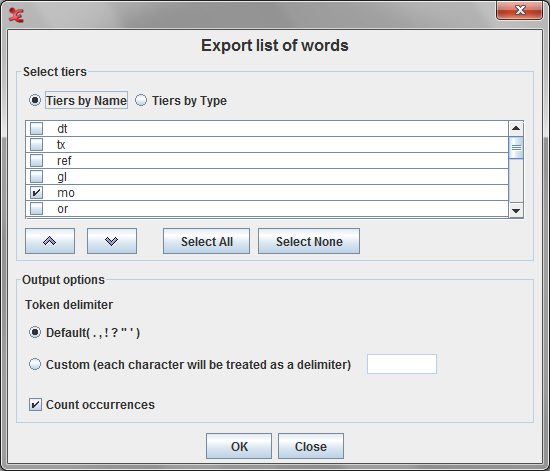
\includegraphics[width=\textwidth]{.\imgpath/Bouda-img9.png}
\caption{Word list export in Elan}
\label{bouda:fig:elanexport}
\end{figure}



Figure \ref{bouda:fig:extract} shows an extract of a sample export file of the Hoc{\A}k corpus. This method allows to some degree the identification of allomorphs of the word/lexeme as mentioned in Section\ \ref{bouda:sec:identificationoflexicaluntis}. The extract shows a list of words with a common prefix \textit{x{\U}n{\U}} `small, little'. Prefixed forms appear elsewhere in the list and have to be searched separately. Alternate stem vowels (long vs. short) will also lead to a separation of list entries with common lexical roots. The user is not able to trace back the entries to the corpus. Once the export is done, the user cannot simply jump to the position within the files where a list entry occurs. The export of the full interlinear context of words/annotations is not possible with Elan.

\begin{table}
\centering
\begin{tabular}{ll|ll}
Word form & frequency & Word form & frequency\\
\hline
x{\U}n{\U} & 1                     & x{\U}n{\U}-{\II}g-n{\A}{\A}gre &1  \\
x{\U}n{\U}-{\II}g & 1              & x{\U}n{\U}-{\II}g-ra & 1            \\
x{\U}n{\U}-{\II}g-i\v{z}{\A} & 1   & x{\U}n{\U}-{\II}k & 6               \\
x{\U}n{\U}-{\II}g-n{\A} & 1        & x{\U}n{\U}-{\II}k-ra &2             \\

\end{tabular}
\caption{Extract from the word list of the entire Hoc{\A}k corpus}
\label{bouda:fig:extract}
\end{table} 

\subsection{Search multiple eaf}

The second feature to be discussed here is the ``search multiple eaf'' option. This search functionality allows the user to search in the domain's eaf files for search terms. Search terms can be regular expressions or raw strings. The only other option in the search dialog is to switch on or off case sensitivity. Figure \ref{bouda:fig:multipleeaf} shows the search result dialog for the search term \textit{x{\U}n{\U}} `small, little'. In this case, the user is able to jump directly to the occurrence of the search term by double-clicking on any entry in the result list. In addition, the user is presented with the annotations before and after the search hit. This search is applied to all tiers in all files. It is not possible to restrict the tiers to search. The user can export the result list in a tab-separated format.

The search results are not displayed in full interlinear context, only a user-defined context on the same tier before and after the search term is shown.

\begin{figure}
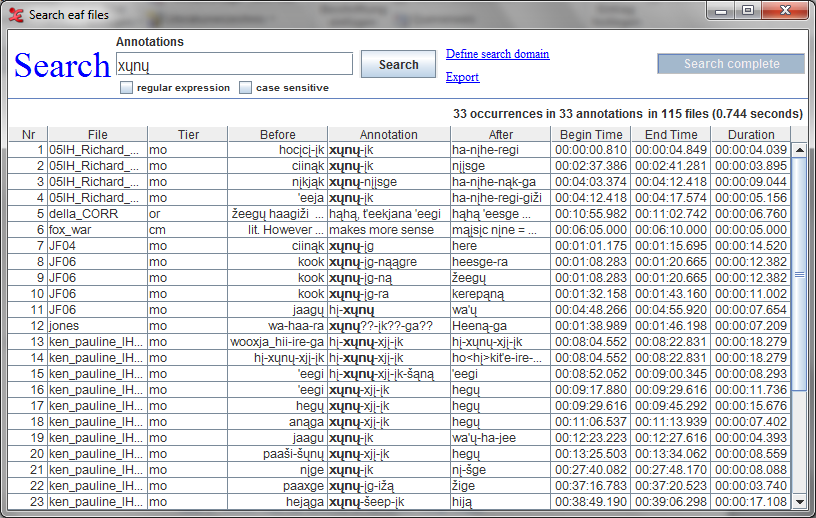
\includegraphics[width=\textwidth]{.\imgpath/Bouda-img10.png}
 \caption{Search multiple eaf in Elan}
\label{bouda:fig:multipleeaf}
\end{figure}



\subsection{Structured search multiple eaf}

Regarding the search typology presented in Section\ \ref{bouda:sec:typologyofsearches} above, the ``structured search'' is the most comprehensive facility for search and analysis in Elan. The ``structured search'' is in itself divided in three dialogs, hence search facilities: a simple substring search over all domain files, the single layer search and the multiple layer search. As only the latter two go beyond the ``search multiple eaf'' option already presented in the previous section, we will be only concerned with the search in layers here.

Figure \ref{bouda:fig:structuredsearch} shows both search dialogs. The left dialog presents a search for \textit{x{\U}n{\U}} in all tiers of the type mo. The ``multiple layers search'' is shown in the right dialog, with sample search for \textit{x{\U}n{\U}} in all tiers of type mo together with an occurrence of \textit{little} in tiers of type ft. In this example, the constraint between the tiers is set to ``No overlap''. The green boxes between search term boxes in the dialog allow the user to set different constraints within and between tiers. Constraints between tiers are concerned with different types of overlap, for example ``Left overlap'' or ``Within''. Constraints within a tier set the a maximum, minimum or exact distance of two search terms within the given tier, in terms of annotation counts or milliseconds within the media file.

 Both dialogs present the results in the lower parts of the dialog as concordances. The user can define the context size of the concordance. An alternative view is given by the ``frequency view'', in which all search hits are listed in a table with a count and a percentage. In both views the user can jump directly to the annotation in the eaf file by double-clicking on the element in the list view. The search results may also be exported to a tab-separated file with all timing and context information.

\begin{figure}
 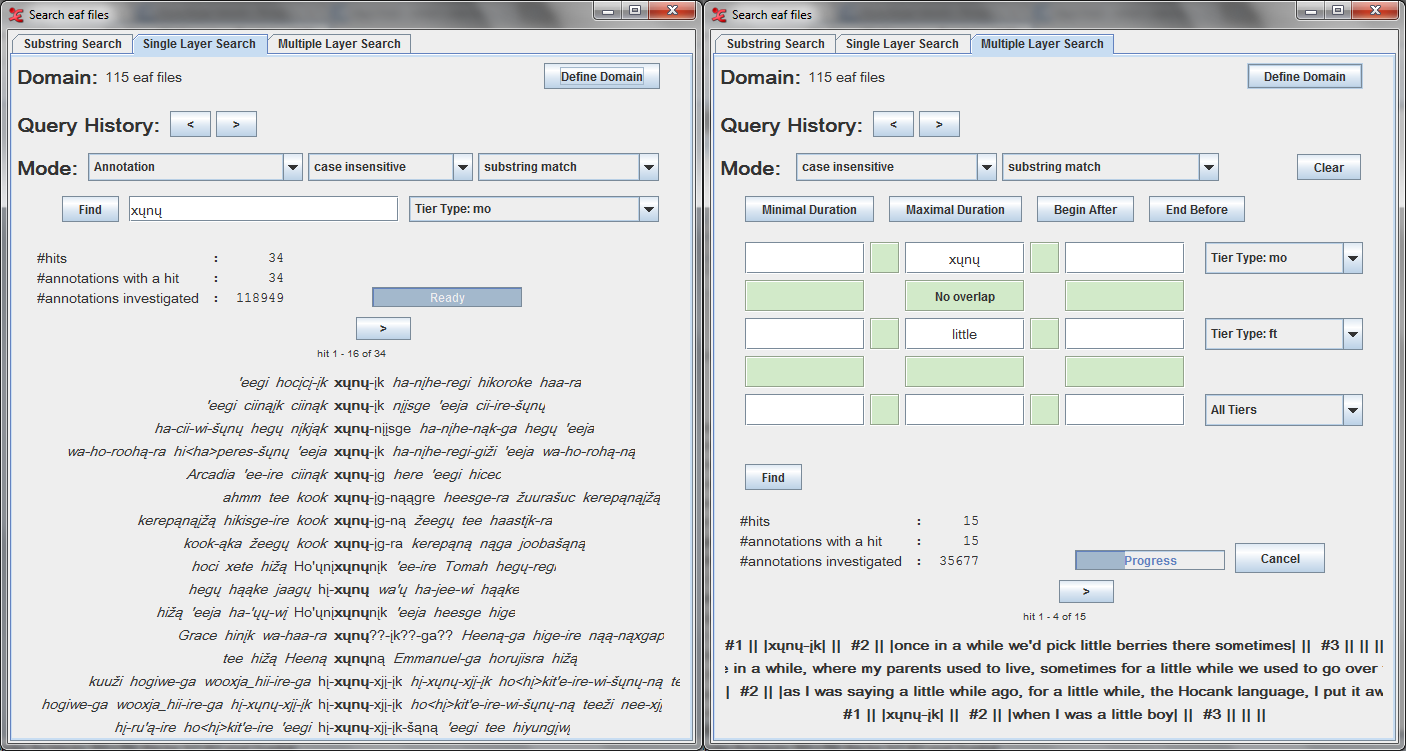
\includegraphics[width=\textwidth]{.\imgpath/Bouda-img11.png}
 \caption{Structured search in Elan}
\label{bouda:fig:structuredsearch}
\end{figure}

\subsection{Summary}
\label{bkm:Ref296713597}

Regarding the maxims in Section\ \ref{bouda:sec:softwarebasesearch}, the software Elan is rated as follows:

\begin{enumerate}
\item \textbf{Search results should be presented as interlinear text:}
It is not possible to view search results as interlinear text in Elan. Elan does not even display the annotation for all the tiers at the location where search strings occurs. Only the context within the tiers that was searched in is displayed. Elan does ignore this value completely.

\item \textbf{The user should be able to find the source utterance in its context in the original file from the search result.} 
The user is presented with a configurable context within the list of search results in the simple and complex searches. The user can click on each element in the list and Elan will open another window with the file of the search hit. The user than has to scroll left and right to see the context of the annotation and utterance within the file. We see problems in usability here, but in general Elan implements this feature.

\item \textbf{The user should be able to search on all existing tiers:}
Elan does allow searches on each tier without restrictions.
\item \textbf{Relationships among search terms:}

 \begin{enumerate}
 \item \textbf{It should be possible to define relationships among search terms on one tier;}
 \item \textbf{It should be possible to define relationships among search terms on different tiers:}

 Elan allows both types of connections between search terms. For some of our users in the project the connection names like ``overlap{\textquotedblright}, etc. were not very clear, so we think that usability could be improved. On the other hand the detailed connection types allow every thinkable search combination for the expert user.
 \end{enumerate}

\item \textbf{The user should be able to search within search results:}
Elan does not allow any further searches on the search result. 

\item \textbf{Search should be possible in a set of files, not only in one file. The more file formats supported, the better.}

Elan support searches in multiple files through its ``domain'' concept. But only one file format is supported directly, Elan's EAF format. The user may search in other file types by importing the files first and save them as EAF files.

\item \textbf{The user should be able to search for substrings in annotations and use regular expressions.}
Elan does fully support regular expressions.
\item \textbf{It is better when the user is confronted with fewer dialogs and windows during one search tasks.}\footnote{This 
 is only an approximation of the quality of the graphical user interface design; a full review is left for future research.}
Elan's search functionality is scattered among several menu options. So, the user has to open several menus and dialogs to try every possible search type. In the case of the export of word lists the user even has to open another application to apply the search. In our view Elan fails regarding this maxim.

\item \textbf{It should be possible to export searches and search results, in order to save and archive them for later reference.} It is possible to export the search results in Elan, but not the searches.
\end{enumerate}

In summary, Elan implements features for 6 of the 9 maxims. Maxims 1, 5 and 8 are violated completely, maxims 4, 6 and 9 only partly or only when we additionally take usability into account (in case of maxim 4). Elan's strength definitely is the structured search that allows advanced search strategies if the user learns about the connection types. Definitely missing is the interlinear view of search results, we also found major restrictions in getting context information from search results. Although the latter is possible, it is quite difficult for the user to get a quick overview of the search result and its context on all tiers at one glance.

\section{The Poio Analyzer for descriptive linguists}
\label{bouda:sec:poioanalyzer}
The development of the Poio Analyzer was started because we felt that Elan was not fulfilling all our needs. The software was planned as a tool for descriptive linguists working with data from language documentation projects from the beginning. Once the search typology emerged during the analysis of the Hoc{\A}k data, it became clear that Elan is not the right tool for a grammar writer to carry out the analysis. The development of the Poio Analyzer did not start from scratch though, as there was already a library for Toolbox and Elan file access (PyAnnotation\footnote{ \url{http://www.cidles.eu/ltll/poio-pyannotation}}) and a morpho-syntactic annotation editor (Poio ILE\footnote{\url{http://www.cidles.eu/ltll/poio-ile}}) available. The first provided a common API to the data files with access to the morpho-syntactic annotation, while the latter already contained a view to display utterances in an interlinear style. Both software packages were developed and used within the DOBES project ``Minderico --An endangered language in Portugal''.\footnote{\url{http://minderico.caorg.pt}} All software packages including Poio Analyzer are available for download on the Poio website\footnote{\url{http://www.cidles.eu/ltll/poio}} and are licensed under the GNU General Public License v3.0. Besides the source code there are installation packages for Windows available.

The following section will describe the user interface of Poio Analyzer, with a focus on the requirements that are missing in Elan and that Poio Analyzer implements. We will then give an outlook on future features that are currently work-in-progress before summarizing Poio's features and rating the software.

\subsection{The User Interface of Poio Analyzer}

Figure  \ref{bouda:fig:poioanalyzer} shows a screenshot of the Poio Analyzer. The main sections of the GUI are marked by numbered boxes. The example data in this screenshot show a search for the regular expression ``\^{}ra\$'' on the morpheme tier, the gloss ``\textsc{def}'' on the gloss tier and the word ``{\textbackslash}bthe{\textbackslash}b'' within the translation. The functionality of each part of the GUI surrounded by boxes is as follows:

\begin{enumerate}
\item Search tabs allow successive searches. Each ``New Search...'' tab filters on previous searches. Tabs allow changing intermediate searches by switching between the open tabs. Results are displayed for the current tab.
\item Input fields for search strings to search in each tier. Allows full-flavored regular expression through the updated Python regex module. E.g. character classes like {\textbackslash}w or {\textbackslash}b fully support Unicode; there is support for Unicode properties, blocks and scripts, etc.
\item Search options:

 \begin{enumerate}
 \item AND: matches, when all search strings of all tiers match.
 \item OR: matches, when one of the search strings matches.
 \item NOT: inverts the search result.
 \item ``contained matches'': this value alters the matches in the word, morpheme and gloss tier. If set, the search strings must match within the same word. Otherwise the search strings can match in the whole utterance. For example: if you search for ``ra'' in the morpheme tier, and for ``\textsc{def}'' in the gloss tier, the normal search will display all matches, where ``ra'' occurs in a morpheme plus all matches where ``\textsc{def}'' occurs in the gloss tier within one utterance. If ``contained matches'' is set the result will only contain matches where a word has ``ra'' in the morpheme tier and ``\textsc{def}'' in the gloss tier.
 \end{enumerate}

 \item Buttons for searches. Searches may be saved and restored; this will save all the search strings of all tabs.
 \item Here you can add or delete files from the corpus. The result view will be updated whenever the file list is changed.
 \item The result view. Matches are displayed in green color within utterances and translations. If there is a match on the word, morpheme or gloss tier the whole word and all its morphemes and glosses will be highlighted in green color. This allows the user to find the matches more easily. All utterances are always displayed with full interlinear annotations.
\end{enumerate}

\begin{figure}
 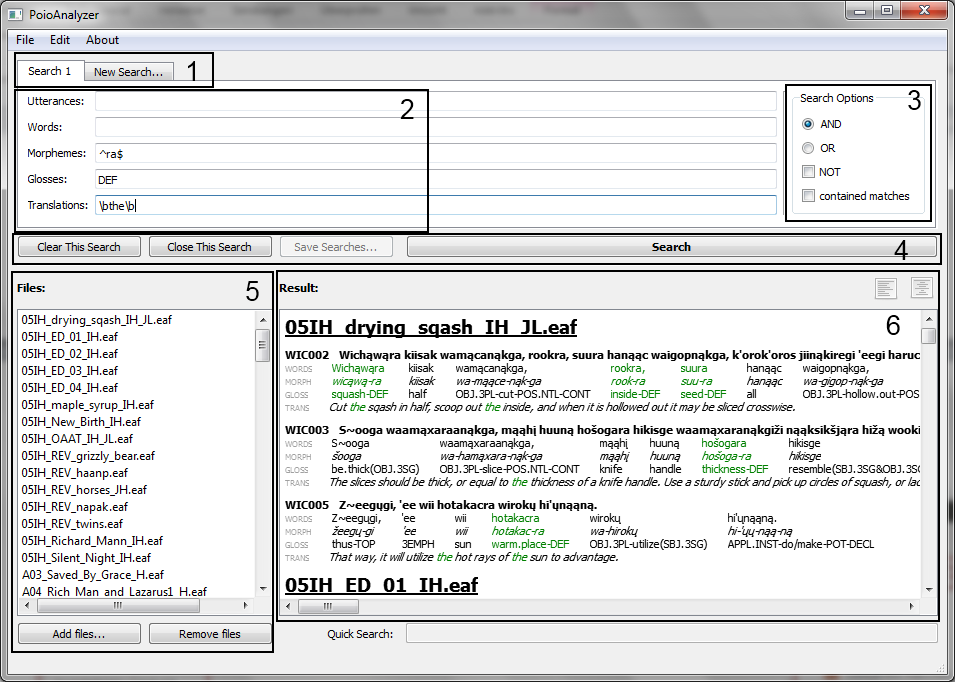
\includegraphics[width=\textwidth]{.\imgpath/Bouda-img12.png}
\caption{The GUI of Poio Analyzer}
\label{bouda:fig:poioanalyzer}
\end{figure}

The screenshot and its description demonstrate two of the most important requirements developed in Section\ \ref{bouda:sec:typologyofsearches}: search hits are presented in full interlinear context and the successive search functionality allows the user to conduct searches on previous search result sets. Both features already add value to the search functionality implemented in Elan and provide easier access to search results regarding the search typology developed in this paper. For example, morpho-phonemic processes as mentioned in Section\ \ref{bouda:sec:morphmebymorphemeglossing} can be analyzed by searching on the utterance and morpheme tier, with a logical AND operation and ``contained matches'' enabled. Another example is the search for word internal morphological structure as described in Section\ \ref{bouda:sec:wordinternalmorphologicalstructure}:  a search for the gloss ``\textsc{fut}'' with results in full interlinear context makes it easier to find out what kind of morphophonemic processes happen between the stems and the grammatical formative or between the combined forms of grammatical formatives. The biggest advantage of Poio Analyzer here is the view of results as interlinear version.

\subsection{Work in progress}

One of the features that were mentioned in Section\ \ref{bouda:sec:poioanalyzer} was the possibility to archive searches and result sets. This feature is currently not available in Poio Analyzer, but we plan to soon release an update that at least allows saving and restoring searches. Other functionality that we are currently working on is:

\begin{enumerate}
\item The possibility to search for set of words, morphemes, glosses, etc. This feature seems critical as it allows for example to search for word classes (e.g. part-of speech) which are not directly derivable from the annotations. In language documentation project there are often preliminary, sorted word lists available, that can be used for this kind of search. In the case of Hoc{\A}k a full dictionary is available, which we will use to search for word classes.

\item On top of this we want to make it possible to add part of speech annotation to the data. In the case of Hoc{\A}k there is part of speech information available in the dictionary. We are currently investigating the quality of part of speech tagging from this dictionary. Part of speech information would allow search for argument structures as described in Section\ \ref{bouda:sec:beyondthewordlevel}.

\item Add statistical evaluation of search result sets. This will be a simple count and percentage value for each tier first. Later, more advanced statistical methods may be added, depending on the needs of the users. The statistical view will also give access to list of words, morphemes and glosses in the result set. Those lists may then be exported and/or used for the ``set search'' described in 1.
\end{enumerate}

In addition to this we are always collecting ideas for improvement from our users. Depending on the complexity and necessity we will implement anything that seems useful to the descriptive linguist.

\subsection{Summary}

Regarding the maxims in Section\ \ref{bouda:sec:softwarebasesearch},the software Poio is rated as follows:

\begin{enumerate}
\item \textbf{Search results should be presented as interlinear text.}Poio does display all search results as interlinear text.
\item \textbf{The user should be able to find the source utterance in its context in the original file from the search result.}Poio does only view the utterance of the search hit. The context of the hit within the utterance is displayed completed, but utterances before and after the search hit are not presented to the user.
\item \textbf{The user should be able to search on all existing tiers.}Poio allows searches over all tiers that are relevant for interlinear texts. Additional tiers (that are not part of the hierarchy of a given utterance tier) are not supported yet.
\item \textbf{Relationships among search terms:}

 \begin{enumerate}
 \item \textbf{It should be possible to define relationships among search terms on one tier.}
 \item \textbf{It should be possible to define relationships among search terms on different tiers.}
 Poio does support both types of relationships, but not as elaborated as in Elan. For example it is not possible to restrict the search on a given tier with information about context size (''[search term 1] with a maximum distance from [search term 2]{\textquotedblright}).
 \end{enumerate}
\item \textbf{The user should be able to search within search results.}This is fully supported by Poio's successive search functionality.
\item \textbf{Search should be possible in a set of files, not only in one file. The more file formats supported, the better.}Poio supports Elan EAF, Toolbox TXT and Kura XML files. Files with different formats may be opened in parallel. The search is carried out over all open files.
\item \textbf{The user should be able to search for substrings in annotations and use regular expressions.}Regular expressions are fully supported by Poio.
\item \textbf{It is better when the user is confronted with fewer dialogs and windows during one search tasks.}\footnote{This 
 is only an approximation of the quality of the graphical user interface design; a full review is left for future research.
}

Poio follows this maxim, it only consists of one dialog.
\item \textbf{It should be possible to export searches and search results, in order to save and archive them for later reference.} Poio does currently not support this feature.
\end{enumerate}

In summary Poio implements features for at least 7 of the 9 maxims. Maxims 2 and 9 are not supported, implementation of features is only planned for future releases. In addition, maxim 3 and 4 are partly violated, as Poio does not support searches on all tiers if they are not part of the interlinear text convention. Combinations of search terms have certain restrictions, especially for searches on a single tier. If we take all the maxims into account Poio supports more of the ideas expressed by the values than Elan. It definitely has an advantage regarding usability, as it was developed as a special purpose tool for search and analysis. Elan, as a general purpose tool, has a lot of other features, like the possible to edit the files during analysis. The possibility to combine search terms in advanced ways is currently a standout feature of Elan.


\nocite{HartmannEtAl2009hocank}
\documentclass{article}
\usepackage[utf8]{inputenc} % please use UTF8 encoding
\usepackage[T1]{fontenc} 
\usepackage{gb4e}

\begin{document} 
% This file was converted to LaTeX by Writer2LaTeX ver. 1.0.2
% see http://writer2latex.sourceforge.net for more info
\documentclass[letterpaper]{article}
\usepackage[ascii]{inputenc}
\usepackage[T3,T1]{fontenc}
\usepackage[english]{babel}
\usepackage[noenc]{tipa}
\usepackage{tipx}
\usepackage{amsmath}
\usepackage{amssymb,amsfonts,textcomp}
\usepackage[top=0.4917in,bottom=0.7874in,left=0.9839in,right=0.9839in,includehead,head=0.4925in,headsep=0.4528in,nofoot]{geometry}
\usepackage{array} 
\usepackage{hhline}
\usepackage{hyperref}
\hypersetup{colorlinks=true, linkcolor=blue, citecolor=blue, filecolor=blue, urlcolor=blue}
\usepackage{graphicx}
\begin{document}
\clearpage\setcounter{page}{1}\pagestyle{Standard}

\end{document}


\end{document}



\glossSTDmode
\setcounter{exx}{0}\setcounter{footnote}{0}
\renewcommand{\thischapteruuheader}{\uhheader{160-178}{4534}}
\renewcommand{\imgpath}{./Drude}
\newpage
\renewcommand\chapname{Wiki/CMS approach, Language Archiving Technology, and TEI}	
\renewcommand\longchapname{Digital Grammars: Integrating the Wiki/CMS approach with Language Archiving Technology   and TEI}
\renewcommand\shortauthor{Sebastian Drude}
\renewcommand\longauthor{Sebastian Drude\\ Max Planck Institute for Psycholinguistics}
\chapter*{\longchapname}
\chapterauthor{\longauthor}
\mytoc{}
 
\begin{abstract}
 Although intrinsically closely related to the new field of language documentation, grammaticography is still mostly oriented to the book model, usually falling short of making use of related digital resources and hypertext functionalities. In this contribution, we show and discuss possible or easily achievable advances that can built on top of existing technology such as Language Archiving Technology as developed at The Language Archive at the MPI-PL: Exemplars and examples can be found in multimedia corpora of natural speech events annotated with ELAN and visualized with ANNEX, words and word forms can be linked to lexical entries in LEXUS online-databases, and the precise meaning of theoretical concepts can be given in ISOcat entries or related terminological databases. Independently from LAT, Wiki-technology provides online collaboration and version control and opens even the possibility to address different audiences in related sets of pages, but also poses challenges for the overall didactic structure of a descriptive work. As one of the formats, at least for export and exchange, the XML-based TEI may provide a suitable framework, although many specialized tags would still have to be introduced and formatting and functionalities for these tags still has to be implemented. Generally, synchronization between different versions (e.g., on-line and off-line) poses the most intriguing difficulties, but the advantages (also in terms of Nordhoff's maxims) of hypertext grammars as proposed here are overwhelming.
\end{abstract}


\section{Introduction} \label{drude:sec:1}

In recent years, core linguistic disciplines such as language description and linguistic typology have been undergoing major methodological changes due to the rapidly developing digital opportunities and a new interest in the world's linguistic diversity, in particular in endangered languages. The emergence of the new field of language documentation \citep{Himmelmann1998,GippertEtAlEd2006} is both result of and driving force for this development which according to some has the potential for an ``empirical turn'' or even ``revolution'' of linguistics and the humanities \citep{Newman2008, Gippert2010,Whalen2004}.

Also computational linguistics (natural language processing) has started to work with data from small languages and to make contributions to language documentation (e.g. \citet{Bird2009}, \citet{BenderEtAl2010clislt}).

While more and more digital empirical data becomes available and used, scholarly work about languages, in particular grammars, is usually still published as paper-oriented texts, mostly as books, book chapters or articles. Connecting scientific texts with their empirical basis and generally with other related resources is still a desideratum; much of the envisaged ``virtual research environments'' still has to be developed.\footnote{\citet{Thieberger2006} presented pioneering work akin to DGs as proposed here. See also \citet{Thieberger2009}.}

The present contribution discusses technology and proposals for an authoring and reading environment for ``digital grammars'', highlighting the potential role of Language Archiving Technology which does not yet include or develop such an environment.\thanks{The 
 ideas put forward in this contribution have been developed and refined in many discussions with several colleagues, all of which I would like to thank for their valuable input. Among these are Anthony Aristar, Helen Aristar-Dry, Jost Gippert, Jeff Good, Alexander Mehler, Sebastian Nordhoff, Laurent Romary, Albert Russel, Nick Thieberger, Dieter Van Uytvanck, Huib Verwey, Menzo Windhouwer, and Peter Wittenburg. It was not possible in each case to recognize a particular contribution by a specific person, for which I apologize. Of course the responsibility for shortcomings is mine alone.} Many of the aspects discussed here exist (or have been proposed) already individually; the goal of this contribution is primarily to provide a survey of the relevant technology, existing or in development, and to propose to combine certain specific aspects and solutions. To the best of my knowledge, several individual features and their combination are proposed here for the first time. The development of a technological solution that includes all of the features suggested here will need at least a medium-sized project with more than one developer and ideally involving several institutions; a project which still needs to find funding. But even at this planning stage the ideas and views put forward in this contribution should serve to stimulate the debate and to gather a group of interested people and institutions.

The focus and general approach of this paper are akin to work by Good, Nordhoff and others.\footnote{See, 
 in particular, \citet{Good2004,GoodEtAl2010,Nordhoff2007tgasg,Nordhoff2007gwea,Nordhoff2007ggwg}.
} 
\citet{Nordhoff2008} introduced a number of (possibly conflicting) values that may govern the development of such a system, and for each value one or several ``maxims'' (roughly, design features) that honour the value. 
Nordhoff refrains [298] from endorsing any of them, but most are indeed pertinent and should be taken into account in one way or another. Wherever appropriate, I will refer to N's values and maxims, presupposing his discussion.\footnote{I 
 usually refer just to the maxims by ``N[ordhoff]'s maxim \#'' without citing \citet{Nordhoff2008} in every instance. A
 list of these maxims is given in the appendix of this volume.
}

Slightly differently from Good and Nordhoff, I here use the term ``grammar'' as representative not only for comprehensive language descriptions but generally for linguistic work based on primary linguistic data (i.e., mostly on recorded speech events as typically obtained in field research), including typological/comparative or more specific descriptive studies. By ``digital'' I refer not only to the distribution form but imply the broad use of information technology and functionalities such as hypertext links inside and outside the document.

\section{Digital (Hypertext) Grammars}  \label{drude:sec:2}
The possibilities of developing grammars as digital (hypertext) documents has been put forward since the late 1990s \citep{Zaefferer1998}, and recently the topic of general and also of digital ``grammaticography'' has gained attention \citep{AmekaEtAlEd2006,Lehmann2004dog,Lehmann2004fg,PayneEtAlEd2007}.\footnote{Particularly 
 relevant was the \textit{Conference on Electronic Grammaticography} organized by Nordhoff at the 2\textsuperscript{nd} International Congress on Language Documentation and Conservation in February 2011.
} 
Nevertheless, there have been only few and partial attempts at developing a digital infrastructure for linguistic research which includes interlinking the linguistic scholarly texts with spoken samples of language use and other resources.

The major special feature of the digital medium is the possibility to \textit{add functionalities} to pages or individual elements of a text. In the case of classical hypertexts, for instance, \textit{links} connect to other parts of the same text or even to other documents, locally or in the World Wide Web. Further functionalities are for instance database queries or playback of multimedia resources. In this way, a text can be embedded into an environment of related external digital resources.

For the purposes of digital grammars as envisaged here, in agreement with \citet{Good2004}, I consider the following complementary digital external resources to be most relevant:

\begin{enumerate}
\item \label{bkm:Ref296272363} a language archive with a corpus of annotated recordings of naturalistic and elicited speech events (Good's  ``texts'');
\item \label{bkm:Ref296272365} a dictionary/lexical database with lexicographic descriptions of individual words and similar units  (Good's  ``lexicon''); 
\item \label{bkm:Ref296272357} a resource where the underlying concepts and the meaning of the applied terms are explained and made explicit  (Good's  ``ontologies'').
\end{enumerate}

These external resources (which can be respectively abbreviated as ``text database'', ``lexical database'' and ``terminological database'') are discussed in section~ in more detail.

Based on these, I propose the following features and functionalities as crucial for a digital grammar (DG):

\begin{enumerate}
\item The DG is, or can be rendered as, a set of organized and interlinked hypertext pages (see Section \ref{drude:sec:4}).
\item \label{bkm:Ref296267835}Recordings of exemplars  (didactic linguistic examples)\footnote{I 
 follow here the terminology of \citet{Good2004}.
} can be replayed together with their annotation.
\item More relevant examples for specific phenomena can be searched in and retrieved from the text database and/or lexical database.
\item \label{bkm:Ref296267849}Individual lexical entries for individual words cited in the DG can be looked up in the lexical database.
\item \label{bkm:Ref296267853}The meaning of technical terms used in the DG can be looked up in the terminological database.
\end{enumerate}

The relations to the three external resources (a), (b), and (c) can be illustrated as in Figure \ref{drude:fig:1}. The main relevant functionalities are represented by arrows: (e) green, (g) yellow, and (h) blue.


\begin{figure}
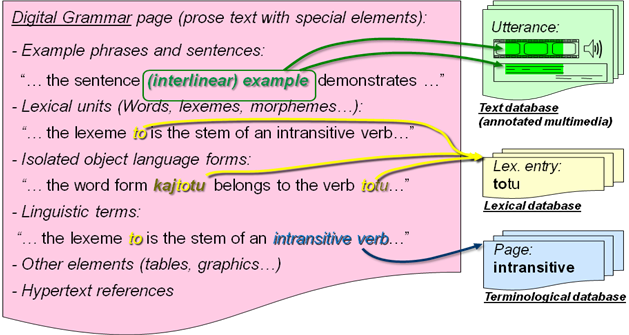
\includegraphics[width=\textwidth]{\imgpath/Drude-img1.png}
\caption{Principal external relations of a DG}
\label{drude:fig:1}
\end{figure}

\section{Language Archiving Technology}  \label{drude:sec:3}
The three external resources proposed to interact with a DG are not new by themselves. In particular, as to the text database, the construction of comprehensive language corpora with annotated recordings of speech events is the very core of language documentation activities as practiced by dozens or even hundreds of projects carried out worldwide in the last 10 years or so.

Digital lexical databases are probably the earliest language resources created with computers in a field research context. Terminological databases, in turn, are better known in the area of natural language processing, for instance for (automatic or manual) translation. They could add value, however, to grammars, which often have been written on two different levels: in many instances, (1)~a specific theoretical conception of a certain domain is explained and the analytical concepts are introduced before [or while] (2)~the specific terminology is applied in describing the language (data) at hand.\footnote{This 
 holds in particular for grammars which are explicitly formulated in a specific theoretical framework. If their terminology is not carefully explained, the grammar runs the risk to be opaque and incomprehensible to anyone not familiar with that particular approach. But also grammars that claim to be ``theory neutral'', mostly using widely used linguistic terms, need to make the exact meaning of the employed analytical concepts explicit because the ``basic'' linguistic terms often have varying or vague meanings.
}
The digital technology allows to keep these two levels apart, so that the DG can focus on the description and analysis, directly employing the terms which are defined and explained in an external terminological database.

One major challenge for all three external resources is: in which form and based on which technology can they be made available for an optimal (in particular, lasting) interaction with the DG? Several solutions may exist for each of them. For instance, there are a few central and several regional language archives, possibly with different standards with respect to file formats and metadata.

Language Archiving Technology (LAT) is a group of interrelated software tools which aims at providing coherent and lasting solutions for the challenges concerning all three external resources identified above. It is developed mainly at the \textit{Max-Planck-Institut f\"ur Psycholinguistik} in Nijmegen (MPI-PL) by what is now ``The Language Archive''. This recently founded unit (earlier the technical group at MPI-PL) is the technological centre of the program ``documenting endangered languages'' (DOBES, funded by the Volkswagen foundation), which was one major reason for developing LAT.

The LAT  suite is comprised of a well-known tool for annotating audio and video language use data, ELAN \citep{WittenburgEtAl2006}, an online service for creating and accessing lexical resources \citep[cf.~LEXUS][]{RingersmaEtAl2007}, and tools for metadata-based access to resources using the IMDI metadata standard \citep{IMDITeam2003}.\footnote{The 
 IMDI-standard is now being superseded by a new CMDI standard developed in CLARIN, the current pan-European initiative to create, coordinate and make language resources and technology widely available and readily useable, one of the core pillars of developing the ``Digital Humanities'' \citet{SchreibmanEtAl2008}.
} 
Metadata can be created with a dedicated editor and now with the ARBIL tool \citep{Withers2009}, and the archive can be browsed and accessed with the IMDI-browser. With the LAMUS tool \citep{Broeder2011}, authorized users can upload resources to the archive while consistency checks are performed. User and access administration is done with the AMS tool \citep{AMS-II}. The resources can be explored online with tools such as ANNEX/TROVA (for multimedia with annotation created with ELAN), LEXUS (for lexical data) and IMEX (for images). Last but not least, the central ISOcat data category registry \citep{Kemps-SnijdersEtAl2009} allows defining concepts to which all resources can refer so that different terminologies can be made interoperable.

Most importantly, the language archive has been built with sustainability and long-term-preservation in mind. It is one of the very few archives which have an institutional commitment (for at least 50 years). It uses persistent identifiers (PIDs, cf.~CLARIN) to ensure that objects can be cited and recovered even if the infrastructure and location of resources changes (cf. N's maxim~24). Several local and regional archives worldwide are adopting the LAT infrastructure. Even if the technology is bound to change, new technology will be backwards compatible and many other independent developments will at least be interoperable with LAT and its successors. 

Crucially, no module for developing grammars (in the broader sense, empirical linguistic work based on speech data) is part of the LAT suite so far, although the basis for building such a platform and integrating it into the existing technology exists. Therefore, LAT is an ideal environment for the development of a digital grammar authoring environment, which is one of the most important points of this contribution. In the next paragraphs, I will discuss the LAT solutions for the three external resources one by one.

The first external resource identified above, the text database for a digital grammar (DG), can be precisely a LAT language archive with IMDI sessions containing ELAN (\texttt{.eaf}) files and the multimedia files they annotate (see figures~2 and~3). An archived ELAN file can be referenced to by its PID, and the ANNEX tool can be used to display and play specific parts of a recording, for instance one sentence of a text, together with its annotation. This allows implementing N's (2008) maxims 1~\&~2 (regarding accountability): each example/exemplar can be traced back to a real utterance. The context of the examples is also immediately accessible in an ELAN file (N's maxim~4). Using searches (e.g., with the LAT online tool TROVA), more examples can be found in the corpus (the text database) and also be displayed in ANNEX (N's maxim~3).


\begin{figure}
\includegraphics[width=\textwidth]{\imgpath/Drude-img2.jpg}
\caption{ A LAT based language archive with an IMDI session }
 \end{figure}



\begin{figure}
\includegraphics[width=\textwidth]{\imgpath/Drude-img3.jpg}
 \caption{An ELAN annotation file displayed in ANNEX}
\end{figure}

Creating and exploring lexical databases (LDs, the second external resource of DGs) is the very purpose of the LEXUS tool. Currently many LDs in LEXUS have been imported from other tools such as toolbox (formerly shoebox), and interchange with other lexical database tools will continue to play an important role.\footnote{The 
 ongoing RELISH project at the MPI-NL, University Frankfurt and Institute for Language Information and Technology at the East Michigan University aims at making different lexical resources, in particular LEXUS (LMF) databases and LIFT-compatible databases interoperable.
}
Still, differently from Toolbox, LexiquePro, FLEX and other lexical tools, LEXUS relies on the ISO standard LMF \citep{FrancopouloEtAl2007}; see also \citet{RingersmaEtAl2010} for LDs and is designed to provide full multimedia support.\footnote{Very 
 recently, the LEXUS tool has undergone a complete re-implementation, and more major improvements regarding user interface and functionalities are foreseen for the next future. For instance, it is planned to integrate LEXUS with ELAN so that semi-automatic glossing of sentences and texts based on lexical data (at least including functionalities known from Toolbox or FLEX) becomes possible.
} 
Although work on a stand-alone version is making progress, LEXUS is fundamentally web-based, and uses also PIDs so that integration with other tools is straightforward. 


\begin{figure}
\includegraphics[width=\textwidth]{\imgpath/Drude-img4.png}
\caption{A LEXUS lexicon}
\end{figure}
 
Finally, the purpose of the more recent ISOcat data category registry is to be a central location where definitions of terms for all areas of linguistics and language technology can be provided so that documents and other resources can refer to them. By defining relations between different entries (the ``substantive'' in one framework can be very close to equivalent to the ``noun'' in another framework), language resources are prepared for the semantic web \citep{W3C2011,GoodEtAl2010}. As such, ISOcat can be a central reference or starting point for the terminological database as proposed here. This holds for Good's 2004 ``general'', ``subcommunity'' and ``local ontologies'' alike, which in ISOcat can be distinguished by creating ``collections'' of terms. The GOLD \citep{FarrarEtAl2003} terms have been included in ISOcat by the RELISH  project and are available as one such selection.

\begin{figure}
\includegraphics[width=\textwidth]{\imgpath/Drude-img5.jpg}
\caption{The ISOcat category registry}
\end{figure}

Possibly, for the purposes of descriptive linguistics, at least some frameworks will need a more integrated terminological resource with richer explanations than the small text-only technical definitions that are usually given in ISOcat. We propose that such frameworks build their own reference system, for instance in the form of a Wiki, but use ISOcat as a point of reference (where short definitions should be provided). But also less theory-specific descriptions should still link their terms to a corresponding ISOcat entry (which generally will exist, at least for most general terms) in order to guarantee interoperability with other resources. The other LAT tools are all prepared to interoperate with ISOcat, so that this appears to be an ideal starting point for the third external resource, the terminological database (for any kind of online documents involving linguistic terminology).

\section{The Wiki/Content Management System approach} \label{drude:sec:4}

As stated in (d) above, a DG should be, or should be able to be rendered as, a set of organized and interlinked hypertext pages. Certainly, however, grammarians, descriptive linguists or typologists are rarely prepared and willing to edit hypertext pages by hand;\footnote{But 
 see the work by Lehmann, presented at the Colloquium on Grammaticography at ICLDC 2.} probably only a minority is regularly using semi-logical mark-up like (La)TeX \citep{Knuth1992}.

Nowadays, websites can be created and edited in Content Management Systems (CMSs) where the content can be entered in an environment similar to better known office software. In particular, the more specialized Wiki-technology is now widely known and used (in rough technical terms, the functionalities of Wikis are a subset of those of CMSs). \citet{Nordhoff2007tgasg,Nordhoff2007gwea,Nordhoff2007ggwg}, elaborating on proposals by \citet{Weber2006}, has proposed and developed ``Galoes'', a Wiki-based online grammar authoring environment.

Indeed, a CMS-based solution has several major advantages, among these:

\begin{enumerate}
\item it is independently existing software, so it has not to be developed and maintained or updated by the developers of the DG system;
\item it usually has version control, which allows inspection of the development of the analysis over time, and going back to previous versions (cf.~N's maxim~7); 
\item it allows collaboration of different users (at different places), and individual contributions are automatically related to their respective authors (N's maxims~11~\& 12 on collaboration); 
\item user-management (usually included) permits to control rights of editing etc. for different kinds of users;
\item it allows for full-text searches, generating an index or dynamic thematic listings of pages (which can be ``tagged'' for this purpose), etc. (N's maxim~15).
\end{enumerate}
On the other hand, there are several major challenges for existing CMS or Wiki systems:

\begin{enumerate}
\item \label{bkm:Ref297464324}most additional functionalities identified in section~2 have to be implemented to ensure integration with the external resources and generally with other (e.g., LAT) tools;
\item \label{bkm:Ref297464521}the Wiki-syntax or display-oriented formatting which usually exists in CMSs is not sufficient for distinguishing the ontological status of the different special linguistic objects;\footnote{For 
 instance, marking an object-language entity with the display formatting ``italics'' does not distinguish between sentences, phrases, isolated word forms, lexemes, syllables etc., each of which may have different associated functionalities. Also, the display formatting may in fact change according to the theoretical framework or the degree of formality/the audience.}
\item \label{bkm:Ref297461869}in particular in a Wiki-like environment, the pages are basically unordered, which impedes a didactical linear arrangement in a sequence of chapters, sections and so forth.
\end{enumerate}

In order to allow solutions for first challenge (f), the CMS has to be extensible (preferably open source). It has been discussed in the previous section that the LAT tools (in particular by using PIDs) are prepared for integration and interaction. 
The second challenge (g) will be discussed in the next section. As to the last point (h) \citet{Nordhoff2008} advocates for nonlinear grammatical descriptions, although admitting that this approach creates difficulties for his maxim 20 (on a didactical presentation).\footnote{The 
 same holds, if less grievously so, for the maxim~21 on the ease of complete reading.
} 
I believe this maxim to be important for most scholarly work, even when using digital technology.

Therefore, I propose, at least as an option, a linear organization in units like parts, chapters, sections, etc. where each organizational unit is represented by one hypertext page; units higher in the hierarchy should contain automatically generated listings of links to their respective sub-units (in addition to an optional introduction or overview). Almost every page should have, then, a clearly defined ``previous'', ``next'' and ``upper'' page,\footnote{Such 
 a linear structure also is the easiest solution for the exhaustive perception problem for readers that which to read the complete description (albeit arguably a minority); cf.~N's maxim~21.
} 
although a reader can follow his own path when reading (in) a DG following links to related but distant pages or using tables of contents and indices (N's maxims~17 \&~18). Of course, the later introduction of an additional page in the middle of a unit, or the splitting of a page into two (while maintaining their place in the linear sequence of pages), or the rearrangement of the order and groupings of pages, are challenges that need to be solved without imposing the burden of manually updating links or unit numberings on the author.

\citet{Nordhoff2008} proposes to `tag' the pages according to their place in one or several standardized outline(s) for grammatical descriptions. This can indeed be useful for readers expecting or familiar with a certain structuring (N's maxim~19), but on the other hand, every linguist may have their own approach and every language may require its own best way to describe it (cf. N's maxim~10 on the author's creativity), so some authors may still choose an individual organization of their presentation. This holds much more for typological work or individual papers on specific aspects of a language. Still, `tagging' pages, e.g. for their relevance and quality (reliability), cf. N's maxims~22 \&~23, is an excellent proposal and easily implemented in a CMS-based DG system. 

Whether one adopts a (possibly standardized) hierarchical and linear organization or not, individual pages in a CMS allow the author to systematically address different groups of readers separately. This has the potential to overcome a notorious problem of grammars (it may occasionally also concern more specific and smaller linguistic scholarly texts): although the readers may be, for instance, laymen, general linguists (such as typologists), or colleagues that share highly specific theoretical assumptions and background (besides readers who may master different meta-languages, cf.~N's maxim~25), there is often only one grammar which either tries to satisfy the different needs in one document (for example by extensive use of footnotes) or else which ignores the needs of one or several groups of potential readers.\footnote{This 
 problem concerns descriptive grammars and is different from the well-known distinction between descriptive and didactic grammars; the latter are a completely different type of text which usually needs a rather different organization.
}

A CMS may be set up so that an author can create and manage several individual hypertext pages that all discuss the same topic, albeit for different readers. The organization into different ``layers'' would be orthogonal to the linear and hierarchical organization, as is shown in~ Figure 6. In this way, a reader could choose a default layer so that the links usually point to respective pages (if they exist) of that layer. For a given chapter or section the reader still may choose to read another alternative version with, e.g., more or less detail.


\begin{figure}
\includegraphics[width=\textwidth]{\imgpath/Drude-img6.png}
\caption{Organization in layers and organizational units (detail)}
\label{bkm:Ref299295833}
\end{figure}

It has been suggested by Nordhoff (maxim~9) that templates be provided by the system and applied by the authors of a DG in order to ease the creation of new pages with grammatical information \citep{Blacktv}. This might be useful for potentially highly uniform pages, such as pages that describe the form and function of individual morphemes in an agglutinative language (or functional particles in an isolating language), and can be implemented with a CMS or Wiki environment. However, I believe that such a formalized approach would be appropriate for only some parts of a comprehensive language description, and even less useful for more specific smaller work (see also N's maxim~10 on creativity, conflicting with his maxim~9).

In any case, most CMSs are configurable and flexible enough to allow for the authoring of linguistic scholarly work --- given the interconnected questions of the data format(s) and the corresponding suitable editing mechanism are solved.

\section{The Text Encoding Initiative} 
There are many different formats of and for digital document, and new formats are developed constantly while others become outdated and, after some years, difficult to access. This holds in particular for proprietary formats such as those generated by commercial office software, which is one major reason why a general authoring environment should rely on open and well documented and widely used formats. Such formats can be developed with XML, the extensible mark-up language, which promises to stay for a long time due to its flexibility to adapt the most different data types, and its wide and growing use.  Also, XML has the advantage of being readable both by humans and by machines, which opens possibilities for a later exploitation of DGs by other applications, and their integration into future larger ``virtual research environments''. This is one of the most promising paths that digital methods currently provide for linguistics \citep{BenderEtAl2010lingo}.

We therefore argue that a DG should have XML as one of its central data formats. We say ``one of'' and not ``the'', because any online authoring environment will certainly conceptually have to deal with several formats, at least some of which will be technically different one from another. For instance, there will be a format for display (e.g., HTML), a format for representation in the computer memory (the internal working format), a format for saving the work into digital file(s) for backup and/or exchange purposes, one for print-outs (e.g., PDF), perhaps another one for distribution in a stand-alone application, maybe still another one for entering and editing of the content by the user (such as Wiki-markup), and so forth. With XML as one basic format, some formats (such as HTML and PDF, perhaps via TeX) are possibly generated by the CMS without need for any further developments. The better structured the XML format, the more likely it is to take over several of these functions, relieving the burden of developing (often error-prone) routines for converting (parts of) the work from one format into another, some of them bi-directional, which are part of the challenges for the development of such an infrastructure. Also, based on XML, the data and description can later easily be used and manipulated for different purposes (cf also N's maxim~26). There are several CMSs that have an underlying XML format (e.g., Mapix, Baryshnikov, generally, see Content Management Directory).

Even if XML as one central format for the DG is granted, there are an infinite number of possibilities for the concrete elements and their structuring. Again, it is advisable to adhere, as far as possible, to existing standards. It seems to me that the standard being developed by the Text Encoding Initiative (TEI) is the most promising candidate, as it is widely recognized, particularly in the humanities, social sciences and linguistics (being used by almost 150 major and minor projects).\footnote{Another 
 candidate is the format used by the XLingPaper project, cf. \citet{Black2009,Black2010,Blacktv,SimonsEtAl2009}. Compatibility and interoperability will have to be carefully checked.
} 
There already exist first attempts at integrating TEI-XML in CMSs \citep{Schlitz2010}.

The TEI guidelines \citep{TEIConsortium2009} specify encoding methods for machine-readable texts, making concrete proposals for XML elements, attributes and their use and arrangement. XML can be the basic format for several purposes, in particular publishing \citep{ReedEtAl2009}. There are specific parts of the TEI guidelines that deal with entities relevant for the linguistic analysis.\footnote{In 
 particular, Section 17.1. ``Linguistic Segment Categories'', but also parts of chapter~8 ``Transcriptions of Speech'' and chapter~9 ``Dictionaries''.
} 
Still, there are potentially many entities which are specific to linguistic descriptions (in particular, interlinear text\footnote{For 
 explorative studies, see \citet{BowEtAl2003tgmilt,BowEtAl2003a4lmilt,HughesEtAl2004}. Also \citet{PalmerEtAl2007} propose a dedicated XML representation of interlinear text. The DG environment should build on this and similar previous work.
}). 
It seems advisable to add to the TEI guidelines a chapter or sections with elements for the specific needs for linguistic description, and there is an interest by members of the TEI consortium in adding this (Laurent Romary, p.c.).

On the other hand, the linguistic terminology varies among linguists and frameworks, and at least for certain parts of the terms applied in a language description this may well always be the case,\footnote{This 
 corresponds to Good's 2004 ``subcommunity'' and ``local ontologies''.
} despite the recent attempts at proposing a basic or universal common set (e.g. by GOLD [see references] or Dixon's ``basic linguistic theory'', cf. \citet{Dixon2010}). Therefore, for each DG the applied elements should be extensible beyond those foreseen by even a dedicated TEI module (cf. N's maxim~10 on creativity). Also, all elements should be configurable with respect to the following properties:

\begin{enumerate}
\item display/formatting (font properties, possible ontological distinctions), which may vary for different layers directed to different audiences (cf. N's maxim~8);
\item primary associated functionality (usually accessible by mouse-clicking on the item);
\item possible additional secondary associated functionalities (possibly accessible by a context menu or similar). 
\end{enumerate}

For illustration, three types of entities are probably referred to in any grammar, and would represent dedicated XML elements with the properties exemplified in Table \ref{drude:tab:1}.\footnote{Note 
 that the ontological type ``syntactic unit'' aims at arbitrary (e.g., inline) quotations of object language syntactic units. The ``see interlinear glosses'' function does not render interlinear text exemplars superfluous; these would continue to be the main type of example which should be displayed as such right away by default.
} 
Similar units and possibly further associated functionalities are needed for many other entity types on the phonetic, phonological, morphological, syntactic and semantic levels of linguistic description.

\begin{sidewaystable}
\begin{tabular}{p{2.5cm}p{4.5cm}p{3cm}p{2.5cm}p{4cm}}
\hline
  Linguistic/\newline ontological Type  &
  Tags and properties  &
  Formatting  &
  Main functionality  &
  Possible secondary functionalities\newline
 (tooltips and the like) \\\hline
  syntactic unit\newline
(sequence of words)  &
\texttt{<dg:Synt.Unit>\newline
 he goes \newline
</dg:Synt.Unit>}  &
 he goes 
 italics, roman &
  play \newline
media file &
see interlinear glosses 

see syntactic tree 

jump to lexical entries for individual words\\\hline
 individual word &
\texttt{<dg:Word>\newline
goes\newline
</dg:Word>}  &
  \textit{goes}
 italics, roman &
  see interlinear glosses for morphs &
jump to corresponding lexical entry (offering choice between homonyms)

play media file if exists\\\hline
  lexical word &
\texttt{<dg:Lex.Word  homonym.number=1>\newline
go\newline
</dg:Lex.Word>} &
 go\textsubscript{1}\textsuperscript{W}
 italics, roman, superscript W, subscript 1 &
 jump to lexical entry
 (taking homonyms into account) &
show meaning 

show word class

show occurrences\newline
of forms of the lexical word in texts\\\hline
  technical term &
\texttt{<dg:term\newline ISOcat="intransitive verb" PID="{\dots}"$>$\newline
intransitive\newline
</dg:term>} &
 intransitive 

 roman, upright\newline
(in formal context maybe sans serif) &
{show definition from ISOcat\newline
(or go to ISOcat entry)} &
go to explanation in theory-specific Wiki
go to page in grammar where this entity is discussed\\\hline
\end{tabular}
\caption{Linguistic entities, their XML representation and associated properties}
\label{drude:tab:1}
\end{sidewaystable}

These associated properties are part of the DG infrastructure and in principle independent of the TEI recommendation for elements and their attributes (or any other XML serialization), although some aspects of the functionalities may depend on the XML structure (such as the representation of homonym disambiguation by an attribute in the case of lexical words in Table \ref{drude:tab:1}).

\section{Versioning and publication} 
As many major reference works in the digital world, comprehensive language descriptions are not limited to static documents but they should be ``living'' --- often they need to be extended and revised as our knowledge about the language increases (cf. N's maxims 5 \& 6). This may hold, albeit in minor extent, also for smaller and more specific digital documents about particular aspects of one language, or for typological work which discusses data from different languages. A CMS solution promises to be an appropriate basis for the implementation of digital grammars as advocated here for the reasons discussed in Section \ref{drude:sec:4} (particularly, version control and management of multiple users). Still, ``living documents'' in general and digital grammars in particular present a number of challenges:

\begin{enumerate}
\item there should be only one central ``master'' instance of the DG which is maintained up to date;
\item other instances and copies, possibly in other formats (e.g., for distribution), should be derived from that master instance;
\item a certain version of the DG (e.g., a copy derived and distributed at a certain point of time) should be a citable reference (N's maxim~24);
\item the DG ideally should be editable when working with speakers ``in the field'' (N's maxim~13).
\end{enumerate}

Two main possible derived formats as suggested in (b) are:

\begin{enumerate}
\item book or paper versions for reading without digital equipment, e.g. in libraries and in the field (N's maxim~27);
\item stand-alone offline digital versions for distribution and reading on computers or similar devices (N's maxims~13 \&~16).
\end{enumerate}

The requirements for these two versions are radically different. The paper version needs a linear order of all pages, good formatting on all levels (individual XML elements, see last section, interlinear texts taken from the annotated corpus, sectioning, cross-references, etc.) and a consistent system of citing elements of the primary data (recordings) and their annotations in an appropriate form. Selected parts of the terminological and lexical databases and of annotated texts (without primary multimedia data) can be included. 

In addition, a stand-alone digital version should try to maintain most of the functionalities of the online DG, and therefore include relevant parts of the text database with their primary multimedia data. This not only needs large storage capacities, it also raises possibly complex issues of reorganizing and redirecting the many links so that they point to offline copies of the associated databases. These issues also turn up when it comes to citing specific parts of the DG and/or their associated databases; the specific version should be identified technically so that the relevant state of the work at the respective point of time can be retrieved although by default external links to a DG and its associated databases may prefer to point to always the current version (cf. N's maxim~6 on actuality).

Requirement (a) and generally principles of global availability suggest that the central master instance be online on some central server, as usually is the case of a CMS or Wiki. One master instance on a central server would also allow for automated backups (N's maxim~14 on safety) and (semi-)automatic curation, e.g. transformation to new formats when current formats become obsolete. Both issues are major challenges for the general goal of data sustainability \citep[cf.][]{BirdEtAl2003}.

However, this requirement conflicts with requirement (d) --- on many field sites there is no access to the internet. Allowing for editable offline instances of a DG posits even more complex problems of linking than in the case of offline distributions for exploring and reading. In particular, the need for synchronization of different versions (typically, an offline instance edited in the field with the central online instance) introduces many complex technical issues. Some may be addressable by using an appropriate XML format (see section~5) and established ``diff'', ``patch'' and versioning software (such as Apache Subversion or similar revision control systems). Others may require ``logging'' of changes and their ``replay'' on the central instance, in particular if changes involve the external databases or major rearrangements of the DG. Although the need for offline editing is obvious for use by field linguists, this feature certainly will take much more time than other aspects of the development of a DG.\footnote{This 
 can be seen by the development of the lexicon software LEXUS at the MPI/TLA: although a known demand since its beginning, the offline version of LEXUS is still in an experimental stage.}

\section{Conclusion}

The time seems ripe for the development of a general environment for digital grammars. Much of the necessary technology is available, in particular the technology for the primary external resources connected to a DG: text, lexical and terminological databases. Specifically, I~have argued that Language Archiving Technology (LAT) provides solutions for many of the required functionalities. The same holds for the internal system of the central part of a DG itself, which can be implemented as a special adaption of a standard content management system (CMS). However, there are specific needs for implementing the necessary functionalities of a DG, which requires proper technical interconnection of the different resources and therefore a more specific mark-up of the main text and special elements of a DG than most CMS systems provide by themselves. In particular, I have argued that one central format of the body of a DG should be XML, as far as possibly adhering to the recommendations of the Text Encoding Initiative (TEI) and perhaps extending them. Other aspects need to be better defined and discussed, in particular the question of a suitable editor.

It seems obvious that developing and implementing such a DG environment is a project which cannot and should not be undertaken by one person, or even a small circle of people. Technical and linguistic knowledge of different areas is needed, and in order to be of use for a larger community, representatives of that community must be involved in the development. On the other hand, one central place where the development takes place seems necessary, in order to guarantee a coherent and integrated (although extensible) system.

The Language Archive, the home of LAT, is the obvious candidate for leading the development and hosting a DG environment as outlined in this contribution. Interested linguists and technologists are invited to get in contact with the author so that a community that leads and accompanies such a project can be formed. 




\newpage
\documentclass{article}
\usepackage[utf8]{inputenc} % please use UTF8 encoding
\usepackage[T1]{fontenc} 
\usepackage{gb4e}

\begin{document} 
% This file was converted to LaTeX by Writer2LaTeX ver. 1.0.2
% see http://writer2latex.sourceforge.net for more info
\documentclass[letterpaper]{article}
\usepackage[ascii]{inputenc}
\usepackage[T3,T1]{fontenc}
\usepackage[english]{babel}
\usepackage[noenc]{tipa}
\usepackage{tipx}
\usepackage{amsmath}
\usepackage{amssymb,amsfonts,textcomp}
\usepackage[top=0.4917in,bottom=0.7874in,left=0.9839in,right=0.9839in,includehead,head=0.4925in,headsep=0.4528in,nofoot]{geometry}
\usepackage{array} 
\usepackage{hhline}
\usepackage{hyperref}
\hypersetup{colorlinks=true, linkcolor=blue, citecolor=blue, filecolor=blue, urlcolor=blue}
\usepackage{graphicx}
\begin{document}
\clearpage\setcounter{page}{1}\pagestyle{Standard}

\end{document}


\end{document}



\glossSTDmode
\setcounter{exx}{0}\setcounter{footnote}{0}
\renewcommand{\imgpath}{./Bender}
\renewcommand{\thischapteruuheader}{\uhheader{179-206}{4535}}
 
\renewcommand\chapname{From Database to Treebank}	
\renewcommand\longchapname{From Database to Treebank: On Enhancing Hypertext Grammars with Grammar Engineering and Treebank Search}
\renewcommand\shortauthor{Emily M.\ Bender, Sumukh Ghodke, Timothy Baldwi, and Rebecca Dridan}
\renewcommand\longauthor{Emily M.\ Bender$^\spadesuit$, Sumukh Ghodke$^\heartsuit$,\\ Timothy Baldwin$^\heartsuit$ and Rebecca Dridan$^\clubsuit$\\
\normalsize $^\spadesuit$University of Washington, $^\heartsuit$University of Melbourne, $^\clubsuit$University of Oslo}
\chapter*{\longchapname}
\chapterauthor{\longauthor}
\mytoc{} 


\begin{abstract}
This paper describes how electronic grammars can be further enhanced
by adding {\it machine-readable grammars} and {\it treebanks}.  We
explore the potential benefits of implemented grammars and treebanks
for descriptive linguistics, following the discursive methodology of
\namecite{Bir:Sim:03} and the values and maxims identified by
\namecite{Nordhoff:08}.\footnote{A
 list of these maxims is given in the appendix of this volume.
}
We describe the resources which we believe
make implemented grammars and treebanks feasible additions to
electronic descriptive grammars, with a particular focus on the
Grammar Matrix grammar customization system
\citep{Ben:Dre:Fok:Pou:Sal:10} and the Fangorn treebank search
application \citep{Gho:Bir:10}.  By presenting an example of an
implemented grammar based on a descriptive prose grammar, we show one
productive method of collaboration between grammar engineer and field
linguist, and propose that a tighter integration could be beneficial
to both, creating a virtuous cycle that could lead to more effective
and informative resources.
\end{abstract}

\section{Introduction}

This paper describes how electronic grammars can be further enhanced by
adding {\it machine-readable grammars} and {\it treebanks}, or sets of
structured annotations produced by the machine-readable
grammars.\footnote{We are grateful to the audience at the Conference on
  Electronic Grammaticography and an anonymous reviewer for helpful
  discussion.  This material is based in part upon work supported by the
  National Science Foundation under Grants No.\ 0644097 and No.\
  0317826, and the Australian Research Council under Grant No.\
  DP0988242.  Any opinions, findings, and conclusions or recommendations
  expressed in this material are those of the author(s) and do not
  necessarily reflect the views of the National Science Foundation.  }
Following \namecite{Good:04}, we understand a descriptive grammar to be
a set of annotations over texts and lexicon, including both prose
descriptions and structured descriptions.  In an electronic descriptive
grammar, annotations are illustrated with exemplars drawn from the text
but are understood to express generalizations over more examples.  This
is illustrated in Figure~\ref{fig:good}, from \citeboth{Good:04}.
Machine-readable grammars can be understood as another kind of
structured description.  Because they are interpreted by computers, they
are required to achieve a higher level of consistency, with descriptions
of various phenomena integrated to form a cohesive whole
\citep{Bender:08}. Implemented grammars can automatically produce
annotations over individual examples, which can in turn be aggregated
and searched \citep{Gho:Bir:10}.  This vision is illustrated in
Figure~\ref{fig:bigpicture}.


\begin{figure}[hbtp]
\centering
\includegraphics[width=.6\textwidth]{\imgpath/Annotation}
\caption{The structure of an annotation \protect\citep{Good:04}}
\label{fig:good}
\end{figure}

\begin{figure}
\centering
\includegraphics[width=\textwidth]{\imgpath/BigPicture3.pdf}
\caption{Schematic view of electronic grammars with treebanks}
\label{fig:bigpicture}
\end{figure}


Our purpose in this paper is to explore the potential benefits of
implemented grammars and treebanks for descriptive linguistics and to
present to the descriptive linguistic community the currently existing
tools which can facilitate their creation.  In \sref{sec:bg}, we
describe implemented grammars and treebanks and give an example of
grammar engineering in the context of endangered languages.
Section \ref{sec:ts} describes treebank search, including use cases relevant
to descriptive and documentary linguistics and how it can be
integrated into an electronic descriptive grammar.  Following the
discursive methodology of \namecite{Bir:Sim:03} and the values and
maxims identified by \namecite{Nordhoff:08}, in \sref{sec:vm} we
explore the impact of augmenting descriptive grammars with treebanks.
Finally, in \sref{sec:gt} we explore the resources which we believe make
implemented grammars and treebanking feasible additions to electronic
descriptive grammars.


\section{Background}
\label{sec:bg}

\subsection{Implemented grammars}
\label{sec:wmb}

Implemented grammars are collections of linguistic rules written in a
formalism that can be interpreted by appropriate software in order to
apply those rules to linguistic inputs.\footnote{Implemented grammars
  of this sort are also descriptive in the sense that they capture
  linguistic generalizations.  For present purposes, we will use the
  phrase {\it (electronic) descriptive grammars} to refer to prose
  statements of linguistic analyses and {\it implemented grammars} or
  {\it machine-readable grammars} to refer to formal sets of rules
  that can be interpreted by a computer.}  These inputs can be sentences of
the language, in which case the goal is generally to find the
syntactic and/or semantic structures assigned to those sentences by
the rules (in parsing).  If the rules are morphological rules, the
inputs are word forms and the outputs morphological analyses of the
word forms.  Phonological rule sets map surface forms to underlying
phoneme or feature sequences.  In many cases, implemented grammars are
reversible, allowing processing that takes more abstract structures
(semantic representations, morphological analyses, underlying phoneme
sequences) and produces surface forms.  Software for working with such
rule sets is most developed for syntax,\footnote{e.g., 
  LKB  \citep{Copestake:02},
  XLE \citep{xle}, 
  TRALE \citep{Meu:Pen:Ric:02}.
}
morphology\footnote{e.g.
 XFST\citep{Bee:Kar:03} and the morphological engine in SIL's FieldWorks,
\citep{Bla:Sim:08}.
} and phonology,\footnote{e.g. XFST} but in the future one
can expect other levels of linguistic structure to receive similar
treatment.  Implemented grammars can be extremely valuable for
linguistic hypothesis testing, allowing linguists to check their
analyses of different phenomena for consistency
\citep{Bierwisch:63,Mueller:99,Bender:08,Ben:Fli:Oep:11} and to
discover counterexamples to analyses in collected texts
\citep{Bal:Bea:Ben:Fli:Kim:Oep:05}.

It is worth noting that while implemented grammars are necessarily
{\it formalized} (i.e., written in some formalism which is precise
enough for a machine to handle), they are not typically {\it
  formalist}.  That is, where a formalist approach to linguistics
attributes explanatory power to formal structures and, as a result,
typically seeks to state theoretical results in the form of
constraints on the allowable formal devices, grammar engineering uses
formal structures in order to state analyses and typically favors
flexible formalisms which allow for the exploration of multiple
analyses \citep{Ben:Fli:Oep:11}.  This practical approach to capturing
linguistic generalizations is therefore not at odds with the goals of
documentary and descriptive linguistics.

Bender's (\citeyear{Bender:08a,Bender:10}) work on developing an
implemented grammar for Wambaya [wmb] on the basis of
\quotecite{Nordlinger:98a} descriptive grammar serves as a proof of
concept of the applicability of the computational tools referenced
above to endangered languages and language
description. Bender (\citeyear{Bender:08a}) reports that in 5.5 person-weeks of
work, she was able to create an implemented grammar on the basis of
Nordlinger's descriptive (prose) grammar that assigned correct
analyses to 91\% of the exemplar sentences in the grammar and 76\% of
a held-out test set (one of the transcribed, glossed and translated
narratives included in Nordlinger's volume).

Our purpose in citing these numbers here is to show the feasibility of
grammar engineering in the context of language documentation and to
emphasize its relative inexpensiveness: The grammar engineering effort
built on Nordlinger's original fieldwork and analysis, and was minor
in comparison, representing about 1/20th of the time.  Furthermore,
this case study illustrates that grammar engineering for language
documentation can be done collaboratively: this methodology does not
rely on individuals mastering both the skill sets required for
linguistic field work and for grammar engineering, a point we return
to in \sref{sec:gt} below.

To make the notion of implemented grammars more concrete, we include a
set of sample rule types from the Wambaya grammar in
Figure~\ref{fig:hcp}.  These types are written in
\tdl\ \citep{Copestake:00}, the formalism interpreted by the LKB
grammar development environment \citep{Copestake:02}, and represent
part of an \hpsg\ \citep{Pol:Sag:94} analysis.  The supertype in this
set ({\tt\small  wmb-head-2nd-comp-phrase}) describes all rules that allow a
head to combine with its second complement regardless of whether it has already
combined with the
first (a key piece of the analysis of Wambaya's nearly free word
order).  The two subtypes integrate the constraints on the supertype
with those on other types to define the head-initial and head-final
variants of the rule (again related to free word order).  The rules
combine a head daughter with a non-head daughter, and match the
constraints on the non-head daughter with the constraints on the
second complement of the head-daughter (through the identity tag {\tt\small 
  \#synsem}). These types inherit from further types which handle
aspects of the rules such as semantic compositionality and ensure that the
non-head daughter is linked semantically to the appropriate role
in the semantics of the head daughter.

\begin{figure}
\centering\footnotesize
\begin{verbatim}
wmb-head-2nd-comp-phrase := non-1st-comp-phrase & 
  [ SYNSEM.LOCAL.CAT.VAL.COMPS [ FIRST #firstcomp, 
                                 REST [ FIRST [ OPT +, 
                                                INST +, 
                                                LOCAL #local, 
                                                NON-LOCAL #non-local ], 
           REST #othercomps ]], 
    HEAD-DTR.SYNSEM.LOCAL.CAT.VAL.COMPS [ FIRST #firstcomp, 
                                          REST [ FIRST #synsem & 
                                                       [ INST -, 
                                                         LOCAL #local, 
                                                         NON-LOCAL #non-local ], 
                                                         REST #othercomps ]], 
    NON-HEAD-DTR.SYNSEM #synsem ]. 
head-comp-phrase-2 := wmb-head-2nd-comp-phrase & head-arg-phrase. 
comp-head-phrase-2 := wmb-head-2nd-comp-phrase & verbal-head-final-head-nexus.
\end{verbatim}
\caption{Sample rule types from Wambaya grammar}
\label{fig:hcp}
\end{figure}


\begin{figure}
\centering
\includegraphics[width=.8\textwidth]{\imgpath/trees}
\caption{Seven analyses of (\ref{ex:wmb1})}
\label{fig:lkb}
\end{figure}

Again in the interests of making the notion of implemented grammars
concrete to readers who have not worked with them, Figure~\ref{fig:lkb}
shows a screen shot of the LKB processing the Wambaya sentence
in (\ref{ex:wmb1}) from \citet[75]{Nordlinger:98a}.

\glossSTDmode
\parbox{\textwidth}{
\begin{exe}
\ex\label{ex:wmb1} \gll
Gujarrarna nyilangunya nga yanybi.\\
two.{\sc ii(acc)} echidna.{\sc ii(acc)} 1.{\sc sg.a-pst} get\\
`I got two echidnas.' [wmb]
\end{exe}
}


The seven trees shown in the figure represent the seven analyses that
the current implemented Wambaya grammar licenses for this sentence.
(Note that each analysis is in fact much more detailed; the trees are
merely abbreviations of larger syntactico-semantic structures which
can be accessed through the software.)  Of these seven, the last
(bottom left) matches the gloss provided by Nordlinger (shown in
(\ref{ex:wmb1})).  In that analysis, the constituent {\it Gujarrarna
  nyilangunya} (`two echidnas') combines with the constituent {\it nga
  yanybi} (`{\sc aux} get') via the {\tt\small  comp-head-phrase-2}
rule.\footnote{This is because the NP `two echidnas' is the second
  complement of the auxiliary+verb cluster `{\sc aux} get'.  The first
  complement of the auxiliary is the verb itself.}



Returning to the goals of integrating treebanks with electronic
descriptive grammars, the examples above highlight two important
points about implemented grammars and treebanks:
%
First, annotations derived from implemented grammars make explicit
ambiguity in natural language that speakers rarely notice and even
linguists often skip over, focusing only on the relevant reading of
the examples they are interested in.\footnote{One way that an
  implemented grammar can be incomplete is by licensing more analyses
  than are actually warranted for a string.  Not all ambiguity,
  however, is spurious ambiguity (i.e., involving
  grammatically ill-formed structures).  Any grammar with reasonable
  coverage will necessarily find multiple legitimate analyses of
almost any grammatical string it can analyze.  One of the lessons
of computational linguistics for linguistics is the sheer amount
of ambiguity in natural language \citep{Abney:96}.} 
In most cases, however,
only one of the analyses will correspond to a pragmatically plausible
reading.  Creating a treebank involves selecting that pragmatically
plausible analysis, as discussed further in \sref{sec:tb} below.
%
Second, implemented grammars and tools like the LKB are not enough
to meet the needs of grammar readers looking to use the annotations
in order to find relevant examples in a corpus.  A separate set of
tools is required which can take the output of the implemented
grammar and the treebanking process and provide search functionality.
Fangorn \citep{Gho:Bir:10} is a treebank search application that fills this 
need, as discussed further in \sref{sec:ts}.


% EB Say something about complementing ts with something that allows
% users to understand the analyses of the examples they find??



\subsection{Treebanks}
\label{sec:tb}

A treebank is a collection of natural language utterances annotated
with tree structures. Traditionally, treebanks have been created by
annotating the tree structures by hand, using a detailed annotation
guide. To speed up the process, the text may be first processed with
software tools such as a shallow parser or chunker, so that most of
the manual annotation consists of correcting and elaborating an
initial structure, rather than writing trees ``free-hand''.  The most
well-known treebank for English, the Penn Treebank
\citep{Mar:San:Mar:93}, was constructed in just such a fashion.  This
manual method of creating a treebank has many drawbacks. The most
forbidding is the amount of time required, even with the first
automatic pass, but there are other problems.  Validity of the
annotation is one: It is very difficult to maintain consistency when
annotating complex structures by hand, particularly when different
phenomena can interact in many ways. Another issue is the static
nature of these treebanks. Given the amount of time and money needed
to create them, once a treebank is annotated, it is rarely updated.
This means that out-of-date analyses are kept, even if later
investigation suggests a better hypothesis.

%% other treebanks, uses of treebanks, problems of hand-annotation
%% annotation guidelines, semi-automatic (ie hand-corrected)
%% staleness of annotations

\textit{Dynamic treebanks}, such as the Redwoods treebank \citep{Oep:Fli:Tou:04},
are produced by a newer method of treebank construction that uses an automatic
parser to process utterances according to an implemented grammar. Manual
annotation is still required, but in this case the annotator selects from the
possible trees produced by the grammar to nominate the most plausible (with
the option of rejecting all trees in case the grammar does not provide
a suitable analysis). Since the
annotator never edits tree structure manually, all annotations in the final
treebank are guaranteed to conform to the implemented grammar.  Aside from the
benefits of consistency and speed, dynamic treebanks also have the advantage of
being easy to update when the grammar changes, as described below.

For this type of treebank, once the text is parsed, the annotator selects the
correct tree by making a series of binary decisions based on so-called parse
discriminants \citep{Carter:99}.  
Figure~\ref{fig:tsdb} shows the interface of
the Redwoods treebanking tool used for this
process, with the trees displayed on the left, and the discriminants on the
right. Each discriminant represents a single aspect of analysis that occurs in
some trees, but not others. These differences could be in the syntactic or in
the semantic representation, where a syntactic discriminant consists of a
grammar rule and the portion of the sentence it is being applied to, and a
semantic discriminant describes a predicate and one of its properties or
arguments. An annotator can click on a discriminant and then select \textit{Yes}
to indicate that it is correct, or select \textit{No} to exclude any trees that
are compatible with this discriminant. Since there are many dependencies between
discriminants, selecting one can entail decisions for many others, meaning
that finding the correct tree may only require a small number of decisions.
These decisions are saved, and can then be used to (semi-)automatically update
the treebank after a change has been made to the implemented grammar. When the
text is re-parsed with the new version of the grammar, the old decisions can be
replayed where applicable, and then the annotator only needs to annotate items
that are still ambiguous after the old decisions have been applied.  In this
way, treebanks can be easily updated to reflect improvements in the grammar
without the need for complete (and costly) re-annotation.

\begin{figure}
\centering
\includegraphics[width=\textwidth]{\imgpath/treebanker}
\caption{Treebanking tool}
\label{fig:tsdb}
\end{figure}

In addition to their use in linguistic exploration, these treebanks can also be
used to build a statistical \textit{parse selection} model
\citep{Joh:Gem:Can:Chi:Rie:99,Tou:Man:Fli:Oep:2005}, which can be used to rank
parser output by probability.  While most human-detectable ambiguity requires
contextual information to resolve, the large majority of implausible analyses
can be ruled out on the basis of sentence-internal patterns.  These patterns are
probabilistic and very difficult to model with hand-written parse ranking rules,
but are well handled by the machine learning (pattern recognition) techniques
prevalent in computational linguistics.  For present purposes, parse selection
is of interest because it makes subsequent treebanking efforts easier.  By
learning characteristics of the trees selected as correct in a first round of
annotation, a parse selection model can be used by the parser to automatically
discard the most improbable analyses before the annotator sees them, speeding up
the annotation process.

\subsection{Summary}

In this section we have provided background on both implemented
grammars and treebanks, with the goal of sketching the technology
and methodology available.  The following section will build on this
to describe how treebanks can be used for linguistic research purposes.

\section{Using Treebanked data}
\label{sec:ts}

Treebank exploration is simplified by the use of specially designed
search tools.  These tools read in treebanked corpora and on request
provide instances of trees, similar to the one shown in 
Figure~\ref{fig:sent-tb}, that match the sought tree-pattern of linguistic 
significance from within a corpus.  Common features of
such tools are: a query language to specify the pattern of
interest and a user-interface to view the matching exemplars from
the corpora.

Treebank search tools such as TIGERSearch~\citep{Lez:Kon:00} and 
TGrep2~\citep{Roh:05} have been available for about a decade now.  
Only recently, however, with the development of Fangorn~\citep{Gho:Bir:10} 
has a solution become available which allows for efficient search 
over large-scale treebanks. 

\begin{figure}
\centering
\scalebox{0.66}{\includegraphics{\imgpath/sentencetreebank}}
\caption{Treebank tree format for (\ref{ex:wmb1})}
\label{fig:sent-tb}
\end{figure}

\subsection{Fangorn}
\label{sec:tss}

Fangorn uses a path-based query language that is
a subset of the LPath query language \citep{Bir:Che:Sus:Lee:Zhe:06}.  For
a detailed comparison of different treebank query languages
see~\citet{Lai:Bir:04}. 

Path query languages are used to specify tree nodes of relevance.  A
path is a sequence of required node labels together with operators
that state the relationship between consecutive labels.  In other
words, the path functions as a linear specification of nodes in trees
of interest. For example, one interesting property of Wambaya is that
modifiers can generally stand alone in argument positions
\citep{Nordlinger:98a}.  A linguist interested in 
sentences with this property might begin with a query like
(\ref{ex:qry1}), which finds all parses where a declarative clause
(label: {\small DECL}) has a complement of a verb realized by a modifier
(label: {\small HEAD-COMP-MOD-2}) below it.

\begin{exe}
\ex\label{ex:qry1}\small
\verb=//=DECL\verb=//=HEAD-COMP-MOD-2
\end{exe}

\begin{table}[tp]
\center{
\begin{tabular}{r l r l}
\multicolumn{2}{c}{\textbf{Vertical navigation}} & \multicolumn{2}{c}{\textbf{Horizontal navigation}} \\[3pt] 
descendant & \verb=//= & following & \verb=-->= \\
ancestor & \verb=\\= & preceding & \verb=<--= \\
child & \verb=/= & immediately following & \verb=->= \\
parent & \verb=\= & immediately preceding & \verb=<-= \\
 & & following sibling & \verb|==>|\\
 & & preceding sibling & \verb|<==| \\
 & & immediately following sibling & \verb|=>|\\
 & & immediately preceding sibling & \verb|<=| \\
\end{tabular}
}
\caption{Query operators and their symbols}
\label{tab:axis-ops}
\end{table}

The operator \verb=//= in (\ref{ex:qry1}) is a \emph{descendant} operator. Table~\ref{tab:axis-ops} 
lists the different query operators in the Fangorn query language.
The operators have been categorized
into two types: horizontal and vertical, depending on whether they
specify dominance or sequential positional constraints. The semantics
of the vertical navigation operators are the same as their definition
in the context of a tree. Similarly, the names for the sibling operators 
are mnemonic for their functions. The
\emph{following} operator specifies that the node to the right of the
operator is temporally after the node to the left of the operator. The
\emph{immediately following} operator specifies that the leftmost descendant of
the node to the right is temporally immediately after the rightmost
descendant of the node to the left of the operator. The \emph{preceding} and
\emph{immediately preceding} operators are the inverse of \emph{following} and \emph{immediately
following}, respectively.

The first operator in the query specifies whether the query pattern
should appear at the root of the tree or anywhere in the tree. 
For example, if query~(\ref{ex:qry1}) started with a {\it child} operator (/) rather than a {\it descendant} operator (//), then it would match only trees in which the topmost node is a declarative clause with a HEAD-COMP-MOD-2 somewhere inside it.


Query (\ref{ex:qry1}) specifies a path consisting of two nodes,
however, paths could contain any number of operator-node pairs. Both
vertical and horizontal navigation operators can appear at any
position in the path. The only restriction is on the first operator in
the main path in the query. It has to be either a \emph{child} or a
\emph{descendant} operator.

An operator in a path specifies the relationship between the node
preceding and following it. In some cases, however, we would want to
specify more than one relationship at a single node. For example, 
we may want to modify query~(\ref{ex:qry1}) so that the head and 
complement positions are irrelevant, which means the node under the
declarative clause could be either {\small HEAD-COMP-MOD-2} or 
COMP-HEAD-MOD-2. Each of the two labels has a \emph{descendant}
relationship with the declarative clause {\small DECL}. Example (\ref{ex:qry2})
describes such a query.

\begin{exe}
\ex\label{ex:qry2}\small
\verb=//=DECL[\verb=//=HEAD-COMP-MOD-2 OR \verb=//=COMP-HEAD-MOD-2]
\end{exe}

Square brackets after any node in a path are called {\it filter expressions},
and can be used to indicate alternatives (a split into two or more possible
paths) or conjoined constraints on a node as shown in (\ref{ex:qry2}). 
%EB: Commenting out because this seems to repeat what is above.
%They could also be viewed as branches of the
%main path at a node, where the branches are the paths specified within
%the filter expression.  
The paths within a filter expression are
connected using logical operators AND, OR and NOT to add
flexibility to the constraints.  Further, since the paths within
filter expressions are themselves paths again, queries can have nested
filter expressions.



Fangorn uses a web-based user interface, where the page
contains a search box and a result display area to show the matching
trees. A screen shot of the user interface for query~(\ref{ex:qry1}) 
is shown in Figure~\ref{fig:ts-web}.
The left-hand top corner of the display area shows the total
number of trees that match the query pattern in the corpus.  The first
page, showing 10 trees, is displayed by default. The user can choose
to navigate to other pages. Each tree may match the query pattern more
than once. Hence, the total number of matches within the tree and the
match currently being displayed is shown at the top of each
tree. Other matches within the same tree can be viewed using the
`$<$' and `$>$' buttons at the top of each tree. The trees are
minimally expanded to show the results in a concise manner, but
additional nodes can be expanded or collapsed in the display.  The
nodes that match the query are highlighted and joined by lines that
denote the operators between the nodes. Each matching tree can be
exported in either a bracketed format or as an SVG image identical
to how the tree is displayed on screen.

\begin{figure}[t]
\centering
\includegraphics[width=.8\textwidth]{\imgpath/searchinterface}
\caption{Fangorn's web interface}
\label{fig:ts-web}
\end{figure}

Fangorn can be used in a number of modalities, including
linguistic exploration, grammar engineering, and cross-linguistic
comparison.

Linguistic exploration can be viewed as a kind of ``exploratory data
analysis'' \citep{Tukey77}, whereby users query for particular
lexico-syntactic patterns in a given language, and, e.g., explore
the productivity of a construction, investigate the interactions between
different constructions, investigate the distribution/behavior of a
given construction across different domains (as instantiated in
different treebanks), or simply observe the distribution of given
lexical items in different syntactic contexts. \namecite{Resnik+:2005} is a good example of this sort of exploration using linguistic structure, although that work was not tied to a descriptive grammar.

Grammar engineers can use Fangorn to validate a new analysis, by
analyzing all instances of the given lexical rule or construction in
trees licensed by a grammar. Traditionally, Fangorn has been
applied to ``gold standard'' disambiguated trees. In indexing a larger
set of analyses licensed by the grammar (e.g., the top-500 analyses, as
selected by a parse selection model), however, it is possible to
retrieve all analyses in which a given pattern occurs, allowing the
grammar engineer to gauge whether an analysis is
adding spurious ambiguity. Fangorn can also aid in the education of grammar
engineers, in exploring how the analysis of a given construction is
manifested in syntactic trees, and comparing this back to the ``source
code'' for the analysis in the grammar files.

Finally, assuming a comparable label set between grammars of different
languages, it is possible to perform cross-linguistic queries to
compare, e.g., differences in right-node raising between English and
German in a data-driven manner. We come back to this briefly in Section \ref{sec:fangorn-fut}.



\subsection{Incorporating Treebank Search in Descriptive Grammars}

\namecite{Good:04} presents a vision of electronic descriptive
grammars as linked to searchable corpora, where exemplars chosen
by the author to illustrate particular phenomena can be linked
back to their original context, and additional examples can
be retrieved from the database.  We see the main benefit of treebanks
to descriptive grammars as enriching the range of ways in which 
examples can be retrieved.  

Treebank search can be incorporated into a descriptive grammar
in two different (and complementary) ways:  (i) The author of the grammar
can include specific ``canned'' queries at various points in order to allow
the reader to retrieve examples with properties relevant to
the discussion  (this would of course be in addition to providing
exemplars, as is usual practice); (ii) The treebank search interface
can be made available to the reader to input arbitrary queries
matching their own interests.  At present, Fangorn allows searching
over tree structures with the nodes labeled by the rule (phrasal or lexical)
or lexical type which licensed them, as well as over the words at
the leaves of the tree.  
%EB: FIXME: Say something about searching over node label
% abbreviations?  e.g., S, NP etc?
For the purposes of inclusion in descriptive grammars, it would be
useful to extend that search capability to include the other
annotations over the data (i.e., glosses and translations).  Longer
term, it would also be interesting to include searches over the
feature structures abbreviated by the tree structures, including
especially the embedded semantic representations.

The addition of ``canned'' queries will be relatively straightforward
(once the implemented grammar and treebank are built), and will most
likely be done in collaboration between the field linguist writing the
descriptive grammar and the grammar engineer developing the treebank
(cf.\ \sref{sec:gt}). The exact mechanism for making the canned queries
and associated results accessible to users of the grammars is open to
debate, but can potentially build off the work of
\namecite{Hashimoto+:2007} on lexical type documentation via
illustrative positive and negative examples.

Making the search interface itself useful to readers will require
documentation.  General documentation about the query language will be
applicable to all such treebank-enhanced grammars, but information about
the implemented grammar licensing each treebank will also be required.
The ``canned'' queries themselves will provide a useful part of this
documentation, serving as models for other similar queries.  In
addition, the documentation should include a glossary of all of the
labels in the treebanks (e.g., names of phrase structure rules, names of
lexical rules, names of lexical types, as well as category labels used).
Ideally, this glossary would include links to the relevant sections of
the descriptive grammar and thus be accessible from those sections as
well (following the links in the opposite direction).

\subsection{Summary}

In this section, we have given a brief overview of Fangorn,
how it can be used to formulate queries, and how those queries
could be used to assist readers of electronic descriptive grammars
in getting information from an associated treebank.  In the following
section we reflect further on how implemented grammars and 
treebanks can help fulfill the goals of descriptive and documentary
linguistics.

\section{Values and Maxims}
\label{sec:vm}

\namecite{Bir:Sim:03} structure a discussion of best practices
for creating portable (and thus useful and enduring) language
documentation around a series of value statements and maxims
that follow from those values.  \namecite{Nordhoff:08} picks
up that discussion with a particular focus on how values
identified by \citeauthor{Bir:Sim:03}
% as well as \namecite{Rice:06},
% \namecite{Noonan:06}, \namecite{Weber:06}, and \namecite{Cristofaro:06}
%EB should read those other sources and make sure
%this presentation makes sense.  Also, Nordhoff has two Rice 2006
%items in bibliography. Make sure this is the right one.
% Resolved: These don't use the value/maxim format, but they are
% relevant as sources for the suggestions in the maxims.  Removing
% the cites here and leaving them later.
influence the form of electronic descriptive grammars and inform the
design of software supporting the development of such resources.
\citeauthor{Nordhoff:08} is focusing in particular on those values
that are relevant to electronic grammars with non-linear
(i.e., graph-like) structure. 

In this section, we explore how the addition of treebanks to
electronic descriptive grammars can respond to some of those values,
with a particular focus on those that treebanks speak to, either
because they can enhance the ability of an electronic grammar to
fulfill a maxim or because they would in fact be problematic in some
way.  Following \citeauthor{Nordhoff:08}, we structure the discussion
according to the general areas of data quality, grammar creation (by
authors), and grammar exploration (by readers).  All of the maxims are
given in the consequent of a conditional with the associated value in
the antecedent, as in \namecite{Bagish:83}, the inspiration for
\quotecite{Bir:Sim:03} approach to discussing these
issues.\footnote{Except where noted, the antecedents and consequents
  are direct quotes from \namecite[308--318]{Nordhoff:08}.  Additional
  citations are provided when \citeauthor{Nordhoff:08} indicated other
  sources for the maxims.  Where there are multiple maxims for the
  same value statement, we have kept them as separate statements or
  merged them into one according to the most convenient structure for
  the present discussion. In \citeauthor{Nordhoff:08}'s terminology,
  `GD' stands for `grammatical description', i.e., what we are
  referring to here as an electronic descriptive grammar.}  This
discussion includes both near-term goals using existing technology as
well as longer-term possibilities.

\subsection{Data quality}

\begin{exe}
\ex {\sc Accountability:} If we value the application of the
scientific method, more sources for a phenomenon are better than
fewer sources (\citeboth[395]{Rice:06}, \citeboth[355]{Noonan:06}).
\end{exe}

This maxim is the most obvious win for treebank and treebank
search enhanced electronic grammars: If an electronic grammar
is paired with a database of interlinear glossed text (IGT), it
is already possible to search for some phenomena in that database.
The trees in a treebank make much more of the structure of the
sentences explicit than even the most meticulous IGT, and thus
treebanks make it possible to more easily find examples of a broader
range of phenomena (cf.\ \sref{sec:ts}).

\begin{exe}
\ex\label{ex:ou} {\sc Accountability:} If we value the application of the
scientific method, every step of the linguistic analysis should be
traceable to a preceding step, until the original utterance of the
speaker is reached.
\end{exe}

As noted above, an implemented grammar requires that the various
analyses it implements be integrated into a cohesive whole.  The
flip side of this is that every tree in a treebank represents several
levels of linguistic structure.  In grammars such as the Wambaya
grammar discussed in \sref{sec:wmb}, these include semantic, syntactic
and morphological analyses.  Thus, to the extent that the reader is
supported in exploring the trees, the trees themselves will help
ground semantic and syntactic analyses in previous steps.  The connection
between the morphological string and the original utterance will have
to be handled outside of the treebank, however.

\begin{exe}
\ex {\sc Accountability:} If we value the application of the
scientific method, the context of the utterance should be retrievable
\cite[450]{Weber:06}.
\end{exe}

\citeauthor{Nordhoff:08} discusses this one in terms of the communicative
context (who's speaking, to whom, with what goals, etc).  We assume that if this
information is documented in the database underlying the treebank, then it
should be accessible from the treebank as well.  However, another issue relating
to context arises for treebanks, namely the importance of preserving the
linguistic context.  All implemented grammars are in fact grammar fragments, and
thus will not necessarily have complete coverage over arbitrary samples of
naturally occurring text.  With reasonably mature grammars there are robustness
strategies \citep{Kie:Kri:Car:Mal:99,Rie:Kin:Cro:Max:Kap:02} that potentially allow for partial analyses
in a treebank, but these are unlikely to be applicable or desirable in this
application.  Thus, a treebank associated with an electronic descriptive grammar
will necessarily have gaps, i.e., sentences which are not assigned any trees. In
order to preserve the linguistic context of the examples which are assigned
trees, and which thus can be retrieved with Fangorn, it will be
important to maintain links between the treebank and the underlying dataset.

\begin{exe}
\ex\label{ex:act} {\sc Actuality:} If we value scientific progress, a
GD should incorporate provisions to incorporate scientific progress.
\end{exe}

\citeauthor{Nordhoff:08} notes descriptive grammars are never
finished.  In the same way, implemented grammars also always have room
to grow.  It is a major benefit of the Redwoods approach
to treebank construction \citep{Oep:Fli:Tou:04} that treebanks can be
cheaply and rapidly updated when the grammar that produced them has
been changed.  Thus modern treebanking methodology makes it possible
for electronic grammars with treebanks to rise to this maxim.

\begin{exe}
\ex {\sc History:} If we value the recognition of the historic evolution
of ideas, the GD should present both historical and contemporary
analyses \cite[360]{Noonan:06}.
\end{exe}

The same software that supports the creation of treebanks
({\small\itsdb}, \citeboth{Oep:Fli:98}) allows for detailed comparisons
between treebanks based on different grammar versions.  The primary
purpose of these comparisons has been to allow grammar engineers
to explore the impacts of various changes they have made to the
grammar, in terms of which items (sentences) are assigned different
(or more or fewer) analyses by one version of a grammar than 
another.  It is possible that this same software could be adapted
to facilitate the exploration of the evolution of analyses either of particular examples
in an implemented grammar, or of classes of examples.  Doing so in a way
that would make it informative for linguists who are not grammar
engineers would, however, require significant additional user interface
effort. 


\subsection{Grammar creation}

The particular maxims that \citeauthor{Nordhoff:08} proposes under
this heading are specific to the design of a grammar-authoring platform
that supports the creation of electronic descriptive grammars, and
therefore don't speak to the creation of implemented grammars. Accordingly,
instead of reviewing \citeauthor{Nordhoff:08}'s maxims, we have
proposed some of our own that concern the creation of implemented
grammars (and thus treebanks), but relate to the same set of values.

\begin{exe}
\ex\label{ex:cc} {\sc Assistance}: If we value speed of creation
and comparability (across grammars), we should seek to provide
means to assist linguists in rapidly creating comparable implemented grammars.
\end{exe}

This is in fact the goal of the Grammar Matrix project
\citep{Ben:Fli:Oep:02,Ben:Dre:Fok:Pou:Sal:10}.  
The Grammar Matrix provides a common core grammar, which defines
things such as the format of semantic representations (using Minimal
Recursion Semantics \citep{Cop:Fli:Pol:Sag:05}), an implementation of
semantic compositionality, and general types of rules and lexical
entries.  In addition, the Grammar Matrix provides a set of libraries
of analyses of cross-linguistically variable phenomena.  These libraries
are developed on the basis of a review of the typological literature,
though of course are not assumed to be comprehensive: the project
always anticipates the addition of new options within a library, as well 
as changes to the core grammar.
The Grammar Matrix is described further in \sref{sec:gt} below.

\begin{exe}
\ex\label{ex:cr} {\sc Creativity}: If we value the individual mind's expressive
abilities, support for creating implemented grammars should
not preclude the linguist exploring alternative analyses in the
implemented grammar.
\end{exe}

The Grammar Matrix is in a sense analogous to the prose templates
that \citeauthor{Nordhoff:08} proposes as part of a grammar authoring
platform.  Both make it easier to create a linguistic resource
(descriptive grammar or implemented grammar), in terms of coverage
of phenomena and in terms of compatibility with the relevant set of
tools.  At the same time, these aids can also have the adverse effect
of limiting creativity or biasing analyses towards those anticipated
by the creator of templates/libraries of analyses.  Compared to prose
templates, Grammar Matrix libraries are more difficult to create
(represent a larger investment of time and effort) and are likely also more limiting.  Both
of these effects follow from the fact that implemented grammars 
require all of their component analyses to interact.  On the one hand,
the grammar engineers constructing the libraries must design them
carefully to be interoperable with all of the options of all of
the other libraries \cite[Ch.\ 2]{Drellishak:09}.  On the other
hand, a linguist attempting to develop an alternative analysis for
one phenomenon will find herself hemmed in to a certain extent by
the decisions made in the analyses of other phenomena.

Nonetheless, we believe that grammar engineering provides a net
benefit for analysis exploration because computers can be harnessed to
test the analyses against large data sets
\citep{Bender:08,Ben:Fli:Oep:11}.  Thus even though it can require
non-trivial work to implement alternative analyses, their relative
advantages and disadvantages can be empirically explored
\citep{Bender:10}.  Recently, \namecite{Fokkens:11} has been investigating
the potential of `metagrammar engineering', or the development of
systems that provide not only implemented analyses of varying
phenomena, but in fact multiple analyses per variant.
\citeauthor{Fokkens:11} argues that this will alleviate the risks of
implemented grammars being shaped by the order in which phenomena are
analyzed.

\begin{exe}
\ex\label{ex:collab} {\sc Collaboration:} If we value the potential
for faster progress when multiple investigators collaborate, we should
develop methodologies and tools which support
collaboration.\footnote{\citeauthor{Nordhoff:08} provides a different
  value statement under the heading collaboration: ``We value
  collaboration and the recognition of the respective contributions of
  the collaborators'' (p.\ 302).  We do not disagree with that value
  statement, but find the one provided in (\ref{ex:collab}) more
  relevant to the present discussion.}
\end{exe}

As will be discussed further in \sref{sec:gt}, grammar engineering for
language documentation is an excellent example of the kind of project
that thrives on collaboration, in this case between one or more field
linguists and one or more grammar engineers.  The grammar engineering
work is dependent on the field work and cannot proceed without data
collection, transcription and analysis done by the field linguist.  At
the same time, grammar implementation allows the hypotheses generated
by both the field linguist and (eventually) the grammar engineer to be
systematically tested against the collected data.  Tools which would
facilitate this kind of collaboration include those which help field
linguists to produce consistent and well-formatted IGT, on the one
hand, and those which make the resulting implemented grammar available
for interactive inspection (such as web-interfaces to parsing and
generation algorithms) on the other.

%% EB: I don't really have anything to say about this one.  Just
%% skip it? Talk about version control?
%% \begin{exe}
%% \ex If we value the safety of data,
%% \end{exe}

\subsection{Grammar exploration}
\label{sub:grammar-exploration}

\begin{exe}
\ex {\sc Ease of finding:} If we value ease and speed of retrieving
the information needed, a GD which has a table of contents, an index
and full text search is preferable.
%EB the following is also in Nordhoff, but we don't really have
%anything to say to it:
%, and a GD that does not require internet
%access is preferable.
\end{exe}

Fangorn is an extremely valuable tool for finding information
within a treebank, provided that readers know how to formulate
the queries they are interested in.  We envision embedding pre-formulated
search queries within the electronic prose grammar (as links that
retrieve additional examples from the database, for example).  An
annotated index of these queries could be a useful source of information
for a linguist seeking to formulate additional queries.  

A second question is how to link back to the relevant parts of the
grammar from the trees in the treebank.  Ideally, each phrase
structure rule, lexical rule and lexical type in the implemented
grammar would be annotated with the phenomenon or phenomena that it
implements.  With such annotations, a reader could move from the tree
assigned to a particular sentence to the relevant discussions in the
prose grammar \citep{Thiebergertv}.  The exact means of encoding these annotations is an
issue for future work.  However, we note here that linking to a
particular prose descriptive grammar is probably a more tractable
problem than producing a general index of a stand-alone implemented
grammar.


\begin{exe}
\ex\label{ex:ff} {\sc Individual reading habits:} If we value the individual
linguist's decisions as to what research questions could be
interesting \cite[402]{Rice:06}, a GD should permit the reader to
follow his or her own path to explore it and a short path between
two related phenomena is better.
\end{exe}

\begin{exe}
\ex\label{ex:mn} {\sc Manipulation:} If we value portability and reusability of
the data, the data presented in a GD should be easy to extract and
manipulate.
\end{exe}


The key issue regarding individual reading habits, according to
\namecite{Nordhoff:08}, is that some readers will be asking how a
particular function is realized within a language, while others will
be interested in the function(s) associated with a particular form.
In this context, the fact that Redwoods-style treebanks (as described
here) include semantic representations is a key asset.  While at
present, Fangorn only applies over syntactic structures, it
can conceivably be extended to searches over semantic structures as
well as combined syntactic/semantic queries.  

Furthermore, if the implemented grammar is made available along with the
treebank, it, too, becomes a tool for both form- and function-based
exploration, greatly enhancing the ways that the data can be
manipulated.  For form-based exploration, the reader can send strings to
the grammar for parsing.\footnote{The grammar will return multiple
  analyses in many cases, but if a parse selection algorithm
  is trained on the treebank, those analyses can be ranked
  by their predicted likelihood.}  For function-based exploration, the
reader would want to use a generation algorithm (e.g., that included
with the LKB \citep{Car:Cop:Fli:99}).  Generation algorithms that
work with Grammar Matrix-derived grammars take as input Minimal
Recursion Semantics representations \citep{Cop:Fli:Pol:Sag:05}, which
cannot easily be written by hand.  However, the Grammar Matrix is
compatible with the LOGON machine translation (MT) infrastructure
\citep{Lon:Oep:Ber:04}.  While it would take additional work to produce
an MT system (notably the writing of a transfer grammar), this could in
principle be done.  In that case, within the coverage of the MT system,
readers could submit sentences in the other language of the MT pair and
retrieve strings in the language being documented.  The trees associated
with those strings could then point into the descriptive grammar (as
above).\footnote{Note that for {\sc quality assessment} (\ref{ex:qa})
  and {\sc accountability} (\ref{ex:ou}), strings returned by the
  generator would need to be flagged according to whether they match
  strings in the collected data or in fact represent generalizations
  based on the hypotheses encoded in the grammar.}


\begin{exe}
\ex {\sc Familiarity:} If we value ease of access, a GD that is similar
to other GDs known to the reader is better.
\end{exe}

Here we must acknowledge that treebanks and implemented grammars
will not be immediately familiar to linguists on first encounter,
and there is work to be done to make them more accessible.  However,
once a linguist has become familiar with one such resource, that
familiarity should be readily transferable to another one constructed
in a similar fashion.  This once again underscores the importance
of tools in promoting standardization (cf.\ (\ref{ex:cc})).

\begin{exe}
\ex {\sc Guiding:} If we value an informed presentation of the data,
the GD should present the data in a didactically preferred way
\cite[401]{Rice:06}.
\end{exe}

\begin{exe}
\ex {\sc Ease of exhaustive perception:} If we value the quest
for comprehensive knowledge of a language \cite[162]{Cristofaro:06}, the
readers should be able to know that they have read every page of the grammar.
\end{exe}

%FIXME: (Before camera ready.) Double check Cristofaro to see if that
%makes sense.

Implemented grammars are intricate objects (full of interconnections)
and the field of grammar engineering is still struggling with
developing best practices for documenting them.  It is unlikely that a
treebank or implemented grammar would assist in the ordering of
information or the creation of paths through a prose descriptive
grammar or with ease of exhaustive perception.  However, by embedding
links to Fangorn in that grammar, the prose descriptive
grammar could become a very effective guide to the implemented grammar
(to the extent that the analyses in the implemented grammar all
directly map to analyses in the prose grammar).

\begin{exe}
\ex {\sc Relative importance:} If we value the allocation of scarce
resources of time to primary areas of interest, the relative importance
of a phenomenon for (a) the language and (b) language typology should
be retrievable (\citeboth[2]{Zaefferer:98}, \citeboth[355]{Noonan:06}).
\end{exe}

There are of course many different ways of defining importance
of phenomena.  If one takes a quantitative approach, a treebank can
be a useful tool in exploring such things. Assuming we have an index
linking grammar rules and lexical entries to phenomena described in the
prose grammar, it should be possible to quantify the text
frequency of each phenomenon.  Likewise, the number of rules/entries
in the grammar which are indexed to the phenomenon would give a 
sense of the degree to which that phenomenon interacts with others.

Regarding cross-linguistic relevance, in the long term, the Grammar
Matrix project has the potential to provide this information:  If
there are many grammars constructed on the basis of the Grammar
Matrix and its libraries (the ``customization system''), we will
be able to quantify the relative prevalence of each choice in each
library, as well as co-occurrence tendencies between the choices.
In addition, it is in principle possible to detect whether 
specific analyses in an implemented grammar remain consistent with
the starting point provided by the Grammar Matrix or required changes.\footnote{Of course, there is also always the influence of the grammar engineer
(cf.\ {\sc creativity} (\ref{ex:cr}) above): a grammar could differ
from the analyses provided by the Grammar Matrix because those analyses
did not work for the language in question, or because the grammar
engineer chose to explore alternatives.}

\begin{exe}
\ex\label{ex:qa} {\sc Quality assessment:} If we value indication of
the reliability of analyses, the quality of a linguistic description
should be indicated.
\end{exe}

The development of an implemented grammar is a fairly stringent test
of the quality of linguistic analyses.\footnote{See also \citet{Maxwelltv}} It is not of course the case
that implemented analyses are necessarily correct.  However, with
implemented analyses it is possible to tell whether analyses of
multiple phenomena are consistent with each other and also the extent
to which the analyses collectively account for the available data (cf.\
Good's concept of {\it internal coverage} (this volume)). \nocite{Good:tv}
That is, the quality of a treebank and its underlying implemented
grammar can be partially assessed in terms of the number of examples
in the underlying database which are assigned a tree.

In order for this assessment to reflect on the prose descriptive
grammar which is the basis of the implemented grammar, at least two
points need to be made explicit: (1) the extent to which the analyses
in the implemented grammar are faithful to the descriptive grammar, and
(2) the extent to which the implemented grammar incorporates all of the
analyses in the descriptive grammar.  That is, the descriptive grammar
could be very comprehensive, but if the implemented grammar does not
include analyses for every phenomenon treated in the descriptive
grammar, treebank coverage will be poor.

Using treebanks to assess the quality of individual analyses
is somewhat more problematic.  The same indexing of implemented grammars
that was suggested for measuring the relevance or importance of
particular phenomena could also be used to estimate the success
of their analysis in implemented grammar.  However, these two
factors are confounded:  A highly central or important phenomenon with
a poor analysis would appear to be relatively unimportant, since the
poor analysis could lead to poor coverage for the sentences with
the phenomenon.  Thus what is called for is an independent way to
measure the frequency of phenomena (perhaps based on interlinear
glossed text alone) and then compare that to the measurements taken
over the treebank.

So far this brief discussion has considered grammar/treebank
quality only in terms of coverage, or the ability to find a correct
analysis for any given example.  Another important measure of grammar
quality, however, is ambiguity: Grammars or analyses which are
underconstrained will produce many spurious analyses.  These will not
be apparent in the final treebank, as they are discarded in the manual
annotation step.  However, the maxim in (\ref{ex:qa}) suggests that the
degree of ambiguity found by the grammar underlying the treebank
should be reported.  In addition, it is straightforward to quantify the
extent to which particular rules and lexical entries contribute to
ambiguity.\footnote{Note, however, if a particular rule is prone
to adding ambiguity, that may not be the fault of the analyses of
the phenomena it currently implements (and thus is indexed for) but
rather the analysis of some other phenomenon which should involve
constraints on that rule but does not.}

Finally, we note that in the development of treebanks for descriptive
grammars, the correctness of a tree is determined by comparing the
semantic representation associated with that tree to the translation
and gloss provided for the example.  Thus to the extent that quality
issues in the descriptive grammar affect the quality of the glossing,
these issues will be masked in measures involving the treebank.

\begin{exe}
\ex {\sc Persistence:} If we value citability \cite[14]{Bir:Sim:03},
in order to facilitate longterm reference, a grammatical description
should not change over time.
\end{exe}

As \nocite{Bir:Sim:03} Bird \& Simons and \citeauthor{Nordhoff:08} note,
the solution to the conflict between this maxim and the one
in (\ref{ex:act}) is to take snapshots which can be the anchors
for citations.  The addition of treebanks to electronic descriptive
grammars makes this somewhat more difficult as the versions between
the treebank (and implemented grammar) on the one hand and the
prose descriptive grammar on the other need to be synchronized.
This is perfectly possible, however, with proper planning.

\begin{exe}
\ex {\sc Tangibility:} If we value the appreciation of a grammatical
description as a comprehensive aesthetic achievement, a GD that can 
be held in the hand is better.
\end{exe}

Implemented grammars and treebanks are only valuable as
computational artifacts, and thus will only be the sort of
thing that can be held in the hand when hand-held devices
are powerful enough to run them.  That said, the addition of
an implemented grammar should not get in the way of the production
of the associated descriptive grammar as book.  In practical terms,
any links to treebank searches that are embedded in prose
chapters should be either stripped or made non-disruptive.
In addition, any links in a printed volume must be stable
links that will continue to function as long as possible.

\begin{exe}
\ex {\sc Multilingualization:} If we value the interest of every human
in a given language, especially interest from the speakers of the language
in question, a GD should be available in several languages, among others
the language of wider communication in the region where the language
is spoken \cite[433]{Weber:06}.
\end{exe}

There are two primary ways in which implemented grammars and treebanks
can respond to this maxim.  The first is to be designed to be able to
incorporate and display glossing of the primary data into multiple
different languages.  The second (and longer term) method is through
the machine translation possibilities discussed in reference to the
values {\sc individual reading habits} (\ref{ex:ff}) and {\sc
  manipulation} (\ref{ex:mn}) above.  It is possible in principle to
set up multiple MT systems between a language being described and
different languages of wider communication.  Furthermore, while there
is additional work required for every language pair, each additional
language pair should require less set up work than the first.

\subsection{Summary}

Our purpose in this discussion has been twofold: On the one hand, by
reflecting on values and maxims, we have proposed a series of design
desiderata for the incorporation of treebanks in electronic
descriptive grammars.  On the other hand, we hope to have provided
arguments in favor of the value of treebanks and implemented grammars
to the enterprise of language documentation and description, and
clarified the role that they can play.

%% In summary, it appears that treebanks will be particularly helpful
%% in achieving the goals associated with the values of ...

The incorporation of treebanks into descriptive grammars is possible
on the basis of existing technology, including technology supporting
grammar development, parsing, generation, treebank creation and
maintenance and treebank search.  This is sketched in the following
section.  The preceding discussion makes it clear that achieving the
full potential of the integration will rely on further advances in a
few areas. These include: methodologies and software support for
indexing components of implemented grammars, support for rapid
deployment of machine translation, and user interface improvements to
make implemented grammars and the analyses they assign to strings more
accessible to non-grammar engineer linguists.


\section{Getting there}
\label{sec:gt}

In the previous sections, we have presented the idea of augmenting
electronic descriptive grammars with treebanks and reflected on how
doing so will help descriptive grammars fulfill the values that 
have been articulated for them.  This section addresses the feasibility
of creating implemented grammars and treebanks and discusses the
resources that are available to assist in the creation of such
resources as well as future directions.

\subsection{The Grammar Matrix}
\label{sec:gm}

Building implemented grammars can be expensive and time-intensive.
The English Resource Grammar (ERG) has been under development since 1994,
and now achieves 62-94\% verified coverage over naturally occurring
corpora from a variety of genres \citep{Flickinger:11}.\footnote{The
low end of that spectrum relates to fairly technical corpora,
including technical manuals and chemistry papers.  Verified coverage
over 80\% is more typical.}  The example of the ERG shows that
this kind of grammar and treebank construction is indeed possible,
but it also suggests that it might be too expensive to be applied
in context of language documentation, as envisioned here.

We contend that it is not, for several reasons.  First, a grammar does
not have to be comprehensive, or even approach the ERG's level of
coverage, in order to be useful.  Even a partial treebank would begin to
yield benefits for linguists searching for examples (though it will be
important to make clear the extent to which the treebank covers the
total corpus, cf.\ {\sc quality assessment} (\ref{ex:qa}) above).
Secondly, it is unfortunately the case that language documentation
projects rarely approach a range of genre diversity in the data
collected that compares to the range of genres the ERG has been tested
against.  A smaller genre range means a more tractable problem for
grammar engineering.  Finally, much of the effort that has gone into the
ERG represents solutions to problems that are not in fact
English-specific, but more general contributions to efficient, implemented \hpsg
parsing.

This last point is the motivation for the LinGO Grammar Matrix
\citep{Ben:Fli:Oep:02,Ben:Dre:Fok:Pou:Sal:10}.  Specifically, the
Grammar Matrix aims to facilitate the development of implemented
grammars in languages without such resources by curating and making
available advances from the ERG and other broad-coverage grammars
developed in the DELPH-IN\footnote{\url{http://www.delph-in.net/}}
consortium, most notably the Jacy Japanese grammar \citep{Sie:Ben:02}
and the German grammar \citep{mueller-s-kasper-w00}.  The Grammar
Matrix consists of a core grammar, shared by all language-specific
grammars derived from it, a series of libraries of analyses of
cross-linguistically variable phenomena, and a ``customization
system'' which allows users to select from among those analyses by
filling in a web-based questionnaire \citep[cf][]{Blacktv}.

The core grammar includes definitions (constraints) that are
hypothesized to be cross-linguistically useful.  The customization
system pairs these with more specialized constraints on the basis of
information collected through the questionnaire. The questionnaire
elicits from a linguist-user typological information of varying
granularity: for example, major constituent word order (including
various flexible word order options), the means of expression of
negation, the range of cases (if any) marked on core arguments, the
possibility of dropping each core argument and information about its interpretation when
dropped.  It also allows users to define classes of lexical items and
morphological rules.  Morphological rule definitions include morpheme
forms,\footnote{These are expected to be regularized underlying forms.
  We follow \namecite{Ben:Goo:05} in advocating for separate
  components for morphophonological and morphosyntactic analysis.
  Various tools exist for creating morphophonological analyzers,
  including XFST \citep{Bee:Kar:03}.} morphosyntactic and
morphosemantic features (case, tense, etc.)\ associated with the
morphemes, and ordering and co-occurrence constraints with other
morphemes (including stems).

This strategy of code reuse necessarily involves taking analyses
developed on the basis of well-studied languages and applying them to
lesser-studied languages.  However, the Grammar Matrix project is
explicitly data-oriented in its approach to cross-linguistic
universals and cross-linguistic variation.  With regards to the
constraints provided in the core grammar, these are treated as working
hypotheses only, ready to be revised (or more precisely made variable
and moved into the libraries) when we encounter languages which
present counter-examples.  The methodology of grammar engineering
allows us to empirically test the applicability of analyses and
determine when an analysis really won't work.  Furthermore, our
library development methodology begins with a review of the
typological literature so that we are working with the most
comprehensive possible view of the range of variation in the world's
languages as we develop the libraries of analyses.

The work on Wambaya cited above \citep{Bender:08a} provides 
a case-study in the feasibility of grammar engineering for language
documentation.  The grammar produced is approximately an order
of magnitude less complex than the English Resource Grammar.
% FIXME: Try to quantify that in terms of types/leaf types/rule instances/lines of code?
Nonetheless, it provided interesting coverage over both the
exemplars cited in \namecite{Nordlinger:98a} and a naturally occurring
text used to test the grammar's ability to generalize beyond the
data used in grammar development.  It was possible to achieve this
level of coverage so rapidly thanks in part to the restricted
range of data being considered (relatively short sentences, relatively
little genre variation) but more importantly thanks to the analytical
work done by Nordlinger.  It is in some ways easier to implement analyses
presented in a descriptive grammar than to work from intuitions about
one's own language combined with analyses gleaned from the theoretical
linguistic literature.  In other words: the original descriptive
work (done in this case by Nordlinger) is the hard part.  When this is
done thoroughly and done well, the grammar engineering is relatively
straightforward.

\subsection{Treebanking Support}

Once an initial version of an implemented grammar has been written, building an
\textit{undisambiguated} treebank is an automatic process that can be easily
initiated using the suite of tools available. Treebanking, the process of
selecting the most plausible tree using discriminants (see
Section~\ref{sec:tb}), requires further effort, but much less than manually
annotating the data. 
%% add something about using the examples from the descriptive data to help?
%%also something about who does the treebanking
While treebanking will always require a human annotator if we wish to
maintain quality, there is some work on automatic methods to help make
treebanking easier.  One method that has proved successful in previous
experiments is to rank the discriminants so as to present those most
likely for an annotator to select at the top of the
list. \namecite{Zha:Kor:10} showed that treebanking speed could be
improved by using the annotation logs of their treebankers to build a
statistical model that ranked the discriminants in the order which an
individual treebanker would be likely to select them. Another method,
called blazing \citep{Tan:Bon:Oep:Fuj:05,MacKinlay+:2011b}, uses
supplementary information available about the text to partially
pre-annotate. In this work, the authors used pre-existing annotations of
parts of speech (in the case of \citeboth{Tan:Bon:Oep:Fuj:05}) or phrase
structure trees (in the case of \citeboth{MacKinlay+:2011b}) to
automatically mark some discriminants, leaving the annotator less
decisions to make, and also found increases in treebanking speed.  Rather
than requiring external information, a third strategy would be to use
all the analyses produced for all items to learn trends in the
analyses. While this information is noisy, the trends from the less
ambiguous items inform the decisions to be made for the more ambiguous
items and this partial information can be used to automatically learn a
probabilistic ranking function to rank all analyses. In this way, we can
prune improbable analyses and in the process accelerate treebanking
\citep{Dridan:Baldwin:2010}.

%%A third strategy is to take advantage of the constrained nature
%%of the grammar, and generate all analyses for a given item. By selecting
%%more plausible analysis from these via heuristics or lexical type
%%assignments, it is possible to automatically learn a probabilistic
%%ranking function to rank/prune analyses licensed by the grammar
%%\citep{Dridan:Baldwin:2010}. This can potentially prune improbable
%%analyses from the parse forest, and in the process, accelerate
%%treebanking, without the requirement for a pre-existing treebank.



%% Not sure if we need this section.  Are there further
%% details on how to make a treebank/how to set it up for
%% treebank search that would be relevant here?
%%
%% RD: I've had a go, but this might be more confusing than beneficial - too 
%% much background required to make the points clear?

\subsection{Future Work on Fangorn}
\label{sec:fangorn-fut}

%% linking, searching across parallel annotations (different layers)
%% looking for examples in another language - GOLD labels?

At present, Fangorn has a query language that is sufficient to express
simple queries using paths and filter expressions. However, for more complicated 
queries with multiple logical operators in a filter expression, allowing
braces to group terms would make queries more expressive.
For example, let us consider query~(\ref{ex:qry2})
and add further conditions that require the search to match only those parses 
where the complement of the verb is realized only by a modifier and not by a
nominal head. We would now have to exclude trees which have a {\small HEAD-COMP-2}
or {\small COMP-HEAD-2} label underneath the declarative clause. Query~(\ref{ex:qry2})
would have to be reframed as shown in (\ref{ex:qry3}). If the grouping of elements,
using braces, were allowed we could rewrite (\ref{ex:qry3}) as (\ref{ex:qry4}), 
which is not only more concise, but is also easier to read. 

\begin{exe}
\ex\label{ex:qry3}\small
\verb=//=DECL[\verb=//=HEAD-COMP-MOD-2 AND NOT \verb=//=HEAD-COMP-2 AND NOT 

\verb=//=COMP-HEAD-2 OR \verb=//=COMP-HEAD-MOD-2  AND NOT \verb=//=HEAD-COMP-2 

AND NOT \verb=//=COMP-HEAD-2]
\end{exe}
\begin{exe}
\ex\label{ex:qry4}\small
\verb=//=DECL[(\verb=//=HEAD-COMP-MOD-2 OR \verb=//=COMP-HEAD-MOD-2) AND NOT

 (\verb=//=HEAD-COMP-2 OR \verb=//=COMP-HEAD-2)]
\end{exe}

Another potential means of grouping terms within a filter expression
would be to take advantage of the types declared in the grammar behind
the treebank, which group together sets of rules.
For instance, there are grammar types in Wambaya grammar, shown in (\ref{ex:gram}) (cf.\ Figure~\ref{fig:hcp}), that 
match the two elements of the filter expression in (\ref{ex:qry4}). Replacing elements in (\ref{ex:qry4}) with their grammar type would allow us to further refine the query to (\ref{ex:qry5}). 
The search tool could itself perform the substitution of grammar types with actual labels 
rather than expect the user to input expanded queries. For this to work, Fangorn 
has to be aware of grammar types and expand them prior to execution.

\begin{exe}
\ex\label{ex:gram}
{\small\tt\small  head-2nd-comp-mod-phrase:

 \{ head-comp-mod-2, comp-head-mod-2 \}}\\
{\small\tt\small  wmb-head-2nd-comp-phrase:

 \{ head-comp-2, comp-head-2 \}}
\end{exe}

\begin{exe}
\ex\label{ex:qry5}\small
\verb=//=DECL[(\verb=//=HEAD-2ND-COMP-MOD-PHRASE AND NOT 

\verb=//=WMB-HEAD-COMP-2ND-COMP-PHRASE]
\end{exe}

The current version of Fangorn operates over the abbreviated tree
structures that are used for presentation purposes. The abbreviated trees are
sufficient to distinguish between competing analyses, but they don't expose all
the information that a user might wish to search for. As mentioned in
Section~\ref{sub:grammar-exploration}, the semantic information embedded in the
tree would provide a useful mode of querying. This provides some interesting
challenges in determining the best way to represent semantic information so that
it can be queried, since a tree structure is not a natural representation for
semantics.  We are currently pursuing two different approaches to this problem:
either trying to find a natural way to represent the semantic information we
have in a treelike form, or alternatively, looking for an intuitive extension of
the query language that would allow querying over a more appropriate 
%graph-like?
representation.

Being able to query the syntax and semantics separately provides different views
and avenues of access to the same data. Likewise, other levels of annotation
that exist, such as glosses and translations, could be useful in finding the
examples that a user requires. A simple extension to Fangorn is planned
to allow different annotation levels to be aligned, so that it is possible to
search using one representation and see how the same data is analyzed at a
different level. A more complex extension would allow a query to filter using
multiple levels of annotation, for example using semantic restrictions to filter
a syntactic query. This extension could require extensive changes to the query
language for a fully general solution, but it might be possible to achieve most
of the desired capabilities by designing a means of specifying metadata about
annotations both within the treebank and in the query language.
%FIXME: Before final version.  I think this point still needs to be elaborated
%a bit more.

Another area of future work for Fangorn is the mapping of labels
onto a cross-linguistic label set, e.g.\ based on GOLD
\citep{Farrar:Lewis:2007}. This would involve aligning individual grammar
rules, lexical rules and lexical types onto the GOLD ontology to mark
features such as verb transitivity, noun case and clause illocutionary
force, while preserving the language-specific rule types and/or more
familiar node labels (e.g., {\small NP} and {\small VP}) as are 
currently used. This would significantly enhance cross-linguistic
treebank search, as the label set would be harmonized to a much greater
extent than occurs using the ``native'' label set for individual
grammars.


\subsection{Virtuous Cycles and the Montage Vision} 

The Wambaya case study described above was an exercise in post-hoc
grammar engineering: The implemented grammar wasn't developed until a
decade after the original field work was complete, and sadly, the
language lost its last fully fluent speakers in that time.  The process
of grammar engineering always raises further questions about the data
(as no grammatical description is ever complete), and the Wambaya case
study suggests that collaborations between grammar engineers and field
linguists could be very fruitful:\footnote{We would like to emphasize that nothing in the
  preceding discussion requires that the grammar engineering and field
  work be done by the same person, and in fact it seems unlikely that many
  people would have the skill sets required for both. Going further,
  it seems like grammar engineering would be a less than efficient use
  of the time of someone who has the skills to do original fieldwork.}
While a considerable amount of data collection and analysis has to
take place before grammar engineering can get off the ground, if the
field linguist is still working with speakers when the grammar
implementation work begins, there is the potential for a feedback loop
that speeds up and strengthens the descriptive work.

The Montage project \citep{Ben:Fli:Goo:Sag:04} envisioned a software
environment which integrated tools for the production of IGT,
electronic descriptive grammars and implemented grammars.  The IGT and
the descriptive grammar would inform the implemented grammar, and even
possibly be input to a system that could automatically create a
partial implemented grammar. The implemented grammar would in turn
feed IGT and descriptive grammar development by locating interesting
exemplars (through Fangorn\footnote{Note that this could even
  be done before the manual annotation step of the treebank
  construction process: the treebank search tools described above work
  equally with undisambiguated sets of trees.}), highlighting
possible inconsistencies in glossing, and testing out analyses.

The Montage project itself was never funded, but nonetheless there is progress
in the direction of this vision, including:

\begin{itemize}
\item Collaborative annotation and descriptive grammar authoring environments,
including GALOES \citep{Nordhoff:07}, TypeCraft \citep{Bee:Mih:09} and Digital Grammar \nocite{Drude:11} (Drude, this volume)
% Check Drude cite to see if it's relevant
% Resolved: Yes, looks relevant.
\item The Grammar Matrix customization system (\citeboth{Ben:Dre:Fok:Pou:Sal:10}, cf.\ \sref{sec:gm})
\item The Redwoods methodology for dynamic treebank construction (\citeboth{Oep:Fli:Tou:04}, cf.\ Section~\ref{sec:tb})
\item Treebank search using Fangorn (\citeboth{Gho:Bir:10}, cf.\ \sref{sec:tss})
\item Machine learning algorithms that learn typological properties
from IGT (e.g., \citeboth{Lew:Xia:07})
\end{itemize}

The Grammar Matrix makes it feasible to create interesting implemented
grammars for languages without large computational resources, while the Redwoods methodology
makes treebank development practical. Fangorn makes the
treebanks useful as resources for readers of descriptive grammars.
The longer term goal of semi-automatic grammar implementation is
supported by the Grammar Matrix and the work of \namecite{Lew:Xia:07}
which suggests that it might be possible to learn answers to questions
like those in the Grammar Matrix questionnaire on the basis of
(sufficiently large) sets of IGT (with sufficiently meticulous
glossing).

\section{Conclusion}

In this paper we have presented a vision of how electronic descriptive
grammars can be enriched with implemented grammars and treebanks, and
described how such a vision is supported by current technology as well
as what future developments could add further value.  Following the
discursive approach of \namecite{Bir:Sim:03} and
\namecite{Nordhoff:08}, we have explored the ways in which implemented
grammars and treebanks can help to meet the values and associated
maxims proposed regarding producing the most useful possible language
resources.  To our knowledge, no such treebank-enhanced descriptive
grammar yet exists, but we hope to see them emerge through the
collaboration of field linguists and grammar engineers.

%FIXME before final version
%\section*{Acknowledgments}

% NSF Grammar Matrix grant
% Fangorn funding?
% Conference audience
% Reviewers
% who else?

\documentclass{article}
\usepackage[utf8]{inputenc} % please use UTF8 encoding
\usepackage[T1]{fontenc} 
\usepackage{gb4e}

\begin{document} 
% This file was converted to LaTeX by Writer2LaTeX ver. 1.0.2
% see http://writer2latex.sourceforge.net for more info
\documentclass[letterpaper]{article}
\usepackage[ascii]{inputenc}
\usepackage[T3,T1]{fontenc}
\usepackage[english]{babel}
\usepackage[noenc]{tipa}
\usepackage{tipx}
\usepackage{amsmath}
\usepackage{amssymb,amsfonts,textcomp}
\usepackage[top=0.4917in,bottom=0.7874in,left=0.9839in,right=0.9839in,includehead,head=0.4925in,headsep=0.4528in,nofoot]{geometry}
\usepackage{array} 
\usepackage{hhline}
\usepackage{hyperref}
\hypersetup{colorlinks=true, linkcolor=blue, citecolor=blue, filecolor=blue, urlcolor=blue}
\usepackage{graphicx}
\begin{document}
\clearpage\setcounter{page}{1}\pagestyle{Standard}

\end{document}


\end{document}



\glossSTDmode
\setcounter{exx}{0}\setcounter{footnote}{0}
\renewcommand{\imgpath}{./Maxwell}
\renewcommand{\thischapteruuheader}{\uhheader{207-234}{4536}}

\renewcommand\chapname{Electronic Grammars and Reproducible Research}	
\renewcommand\longchapname{Electronic Grammars and Reproducible Research}
\renewcommand\shortauthor{Mike Maxwell}
\renewcommand\longauthor{Mike Maxwell\\ CASL/University of Maryland}
\chapter*{\longchapname}
\chapterauthor{\longauthor}
\mytoc{}
 
 
\begin{abstract}
It is time for grammatical descriptions to become reproducible research. In order for this to happen, grammar descriptions must be testable, not only by the original author, but also by other linguists. Given the complexity of natural language grammars, and the ambiguity of prose descriptions, that testing is best done using computational tools to verify a computationally implementable grammar. At the same time, grammars need to be useful---and testable---for the foreseeable future; that is, they must be archivable. Yet if a computational grammar is tied to particular computational tools, it will inevitably become obsolescent. This paper describes a means of creating computationally interpretable grammars which are \textit{not }tied to particular computational tools, nor (to the extent possible) to any particular linguistic theory, and which can therefore be expected to remain useful into the future. In order to make such formal grammars simultaneously understandable to humans, they are embedded into descriptive grammars of a more traditional sort, using the technique of Literate Programming. The implementation of this technology for morphology and phonology is described. It has been used to create morphological grammars for Bangla, Urdu and Pashto which are both human-readable and computationally testable.
\end{abstract}

\section{What can be new about grammars?}


\begin{quote}
An article about computational science in a scientific publication is not the scholarship itself, it is merely advertising of the scholarship. The actual scholarship is the complete software development environment and the complete set of instructions which generated the figures. \citep{BuckheitEtAl1995}
\end{quote}

Of all the methods for documenting and describing languages---the creation of written corpora for linguistic purposes, lexicography, grammatical description, and audio and video collection---it is grammar writing that has the longest history. Grammars of Sanskrit, Tamil, ancient Greek, and Latin date back thousands of years.\footnote{This
 material is based upon work supported, in whole or in part, with funding from the United States Government. Any opinions, findings and conclusions or recommendations expressed in this material are those of the author, and do not necessarily reflect the views of the University of Maryland, College Park and/or any agency or entity of the United States Government.
} 
Oddly, the method for writing grammars has changed little; the invention of glossed interlinear text has been perhaps the most noticeable advance. Even the advent of the computer age, which revolutionized lexicography and corpus creation, and made audio and video documentation practical for the first time, has not significantly changed the nature of grammars. For the most part, grammars continue to be a catalog of the various constructs of the language: noun formation, noun inflection, the order of words in the noun phrase, and so forth, augmented by examples, generally from corpora.  All this could be done just as well on paper as on a computer.

It is true that grammar writing has become easier. Grammar authors can draw from the entire set of characters encoded in Unicode, something which was painfully difficult in the era of typewriters, and often inaccurate when typeset by someone unfamiliar with the language. Modern grammar writers are also blessed with the ability to find examples more easily now that the corpora are on computers; and often these corpora are already stored as interlinear text. Whether the interlinearization has been done consistently has not always been easy to verify, even when the interlinearization was done on computers. But even this is becoming better; SIL's Toolbox has an ``Interlinear Verify'' mode, which flags annotations that don't match lexical entries, and SIL's Fieldworks Language Explorer (FLEx) maintains consistency between the lexicon, grammar, and the interlinear text. Finally, there are now checklists of phenomena to be covered, and often grammars of related languages to draw inspiration from.

While making grammar writing easier is a laudable goal, I believe that a more significant step would be for the resulting grammatical descriptions themselves to change: grammars as language descriptions\footnote{An
  anonymous reviewer has pointed out that there are other sorts of grammars besides rule-based descriptions, including studies of the historical development of grammatical features, typological comparisons, analyses intended to explicate or improve the coverage of a particular theory, and comparative grammatical studies across related languages. In contrast, this paper discusses the grammatical description of a single language, with emphasis on observational adequacy.} must become instances of reproducible research. That is, it must be possible for the reader---indeed, for future generations of linguists---to verify that the grammar is correct, i.e. that it actually describes the language as its author claims. 

One significant step towards this goal has been what I will call ``write-time'' links: links from the examples in the grammar to the location in an electronic corpus from which the author copied them \citep{Nordhoff2008,Thieberger2009}. This allows the reader to view the author's example in context. Indeed, it should be possible to have links to the point in the original audio or video from which the example was transcribed, in principle allowing the grammar user to verify the transcription as well.

Going beyond these author-provided ``write-time'' links to examples, a further step towards reproducible research would be to enable search for grammatical constructions at ``read-time,'' i.e. when the user is reading the grammar. To my knowledge, this innovation has yet to be  implemented. It would require either annotation of a fixed corpus for all the grammatical constructs described in the grammar, or else an on-the-fly grammatical analysis and search facility \citep{Thiebergertv}. The latter method would be superior, since it does not depend on the authors' bias as encoded in the annotated corpus. Furthermore, it would allow searching for grammatical constructions not only over the corpora provided with the grammar, but over any additional corpora that the reader may have access to. 

Several requirements must be met in order to do read-time grammatical search over an arbitrary corpus:

\begin{enumerate}
\item For languages with significant inflectional morphology, there must be a morphological parsing engine. 
\item If the grammar describes syntax, a syntactic parsing engine will also be necessary.
\item The grammar must be represented in a way in which it can be used by the parsing engine(s).
\item There must also be a lexicon compatible with the grammar. Specifically, the grammar and lexicon must use interoperable coding for parts of speech, conjugation or declension classes, etc.
\item A tokenizer must be available, to convert the text into tokens which a parser can deal with. There may also be a need for lower-casing words in scripts that make case distinctions.
\item The corpus must be encoded in the same way as the grammar and lexicon, and use the same writing system (or else it must be possible to convert between encodings and writing systems).
\item Finally, the reader will need a tool which can search through the structures output by the parser.
\end{enumerate}
There are also problems of ambiguity resolution; parsers can be expected to frequently return multiple  parses  \citep[cf][]{Bendertv}. Indeed, even tokenization may be ambiguous.

While ``read time'' search for grammatical constructions is not, to my knowledge, currently possible, I believe it is a desirable goal, for without it the reader is forced to accept at face value the author's description of the language; there is no way to verify the grammar.

This paper describes some steps towards this goal. But first, a discussion of why this goal is important.

\section{Archivable research}
\citet{BirdEtAl2003} drew the attention of linguists to the need for language documentation and descriptions to be archivable. They argued that digital copies of lexicons and texts should be preserved in plain text formats, as opposed to binary formats (such as proprietary database or word processor formats); and in particular, they advocated the use of XML and Unicode. While Bird and Simons said little about how to make grammars archivable, much the same case could be made for descriptive grammars: preservation in XML/Unicode formats is preferable to archiving them in proprietary word processor formats. 

But there is more to be said about grammars. Since at least the 1980s, it has been possible to write grammars in computer-readable format, such that the rules could be turned into a parser and applied to texts. For example, SIL released the AMPLE parsing engine\footnote{I
  make a distinction between a generic {\textit{parsing engine}}, which may be suitable for grammars of a wide range of languages, and a {\textit{parser}}, which is the application of a parsing engine to a particular language. Parsers are usually built from three parts: the generic parsing engine, a language-specific grammar in a format readable by the parsing engine, and a language-specific dictionary, also in a format readable by the parsing engine.
}
\citep{WeberEtAl1988}, which has subsequently been used to create morphological parsers for many minority languages; other morphological and syntactic parsing engines have become available since then. Bird and Simons did not touch on how (or whether) computer-readable grammar rules for such parsers should be preserved. However, \citet{AmithEtAl2005}, \citet{MaxwellEtAl2005} and \citet{MaxwellEtAl2008} discuss the following problem: while we can preserve the grammar rules that could be used by this or that parsing engine, the parsing engines themselves---like any software---will eventually become obsolete. The question then is how computer-readable grammar rules, suitable for parsing corpora, can be archived. In particular, how can we write grammars incorporating such rules in a way that the grammars will be usable long after the original parsing engine has become obsolete?

The work presented here builds on these issues of archivability, but expands on them by considering how making a grammar including computer-interpretable rules archivable also contributes to making such a grammar an instance of reproducible research. I now turn to that issue.

\section{Reproducible research}
\begin{quote}
  Abandoning the habit of secrecy in favor of process transparency and peer review was the crucial step by which alchemy became chemistry \citep{Raymond2004}.
\end{quote}

A fundamental requirement of modern scientific research is that the results be reproducible. This can of course mean different things in different sciences; for medical research, it generally means that the application of a treatment to a different group of patients will lead to similar statistical results. But in sciences like astronomy, where an event like a nearby supernova may not be repeated for centuries, it means being able to reproduce analyses from an archived set of data. Language description has elements of both of these kinds of research. For many languages, it is possible to collect additional data, which may be used as additional test cases to confirm or refute a grammatical analysis. But it may be difficult to collect new data from ``exotic'' languages, and impossible with extinct languages, so that reproducibility in such cases means being able to verify that the structures of a fixed corpus can be generated from a lexicon and rules. 

In a sense, linguistics has long been about reproducible research. Grammars have included examples, often in the form of interlinear text, presumably intended not only to illustrate the abstract grammar rules, but also to allow the reader to verify the rules. In some cases, text corpora are published together with the grammar; recently, \citet{BahraniEtAl2011} included a small corpus of test sentences they used to evaluate their syntactic parser. But therein lies the problem: while it may be possible to verify a rule, or a small set of rules, on a few cases, verifying all the rules on all the examples of the grammar, or worse on an entire corpus, is beyond the patience or even ability of most of us. Languages and their grammars are simply too complex; and as a result, research in linguistics is all too often not verifiable in practice. Indeed, with rare exceptions (such as D. Payne's 1981 grammar of Axininca Campa), published grammars are not explicit enough to support verification. \nocite{Payne1981}

In addition to the fact that grammars are often too difficult to test by hand, two other factors make it virtually impossible for traditional descriptive grammars to constitute reproducible research. First, even the best of grammars generally have gaps in coverage. This is of course true for syntactic grammars, but it is also true for morphological grammars of languages with complex morphology. As \citet{Bauer2010} writes, 
\begin{quote}
 reliance on grammars is not sufficient to give completely accurate data... Descriptive grammars rarely exemplify derivational patterns in any detail, rarely say what is productive and what is not, rarely tell you whether the examples they provide are regular or not, and typically provide lexicalised examples. In other words they do not usually provide precisely the kind of information that the morphologist would like to know about.
\end{quote}

Second, the fact that descriptive grammars are themselves written in ordinary languages such as English means that they are inevitably ambiguous. The problem of ambiguity has been discussed for decades in the context of writing specifications for computer programs; see e.g. \citet{Abbott1983}, \citet{Wiegers2003}, \citet{Meyer1985},  \citet{BerryEtAL2003}, and \citet{KamstiesEtAl2003}. The situation is no different, in my experience, for grammar writing; grammatical descriptions are unclear and ambiguous in unforeseen and probably unforeseeable ways. Experience by our team of grammarians at the University of Maryland has found many examples of unclear writing, even in the best of grammars, resulting in our needing to determine what is really going on in the language by consulting other grammars, talking with other linguists working on the languages, and doing our own fieldwork and corpus research. These problems will not go away by trying to write more clearly. The fact that natural language is not sufficiently clear and unambiguous is one of the reasons that natural languages are not, despite years of trying, used for programming computers. Rather, making grammar writing truly reproducible requires that we have an unambiguous way of expressing grammar rules and constraints: a formal grammar, analogous to a computer programming language. 

For these same reasons,  in many scientific fields the term ``reproducible research'' has come to mean something like the following :

\begin{enumerate}
\item Publication of an analysis in more or less the usual form, such as an article in a journal or conference proceedings.
\item Publication of the data used in the analysis in downloadable form.
\item Publication of the software used to perform the analysis in downloadable form. 
\end{enumerate}

This form of reproducible research thus differs from simply data archiving in that not only the data, but the software used for analysis, is made available to other researchers. The analysis described in natural language provides an easily read view of what the authors did, but the published software and data provide the final complete and unambiguous description with which their claims can be verified.

Reproducible research of this sort is often documented by using Literate Programming \citep{Knuth1992} to produce a ``compendium,'' a computer-readable version of the document combining a textual description for human consumption with the software program for computer consumption \citep{GentlemanEtAl2004}; that is, parts (1) and (3) above, and sometimes the data (part 2). This compendium can be obtained by other researchers, who can extract software for verification against data, whether data contained in the compendium, or other relevant data.

In the Literate Programming paradigm, the ordinary published paper (item (1) in the above list) can be produced as a readable ``view'' of this compendium document, by an automatic conversion process.  In fact, it is possible to produce multiple print views from the same compendium; a standard print view might include the program code used to analyze the data, while a view for publication in a conference proceedings might omit this code because of page limitations.

Literate Programming has been used to publish reproducible research in geophysics \citep{ClaerboutEtAl1992}, bioinformatics \citep{GentlemanEtAl2004,Hothorn2011}, epidemiology \citep{PengEtAl2006}, signal processing \citep{BuckheitEtAl1995,VandewalleEtAl2009}, statistics \citep{Leisch2002,DonohoEtAl2009,LenthEtAl2011}, econometrics \citep{KoenkerEtAl2009}, and other fields.

Moving in this direction, as of 2011 National Science Foundation grant proposals must include a data management plan (\url{http://www.nsf.gov/pubs/policydocs/pappguide/nsf11001/gpg\_2.jsp\#dmp}). While this addresses the availability of the data leading to an analysis, it does not attain the full goal of reproducible research. Specifically, it does not require publishing the computational methods used to process the data. Some journals have accordingly gone further, encouraging authors to submit their articles as true reproducible research using Literate Programming: 
the {\textit{Annals of Internal Medicine}} \citep{LaineEtAl2007};
{\textit{Biostatistics}} \citep{Peng2009};
{\textit{The Insight Journal}} (see \url{http://www.insight-journal.org/});
{\textit{Computing in Science and Engineering}} \citep{FomelEtAl2009}; and 
{\textit{IEEE Transactions on Signal Processing}} (see \url{http://www.signalprocessingsociety.org/publications/periodicals/tsp/}).
The publisher Elsevier has sponsored the ``Executable Paper Grand Challenge'' at the The International Conference on Computational Science in Singapore in June 2011. For linguistics, the new {\textit{Journal of Experimental Linguistics}} (\url{http://www.elanguage.net/journals/index.php/jel/index}), part of the LSA's eLanguage initiative, could begin to address these issues.

At the University of Maryland, we have begun using Literate Programming to document grammars of natural languages, particularly the morphology and phonology of these languages, as reproducible research. As with other Literate Programming approaches, our grammars consist of two interwoven parts: one is a traditional descriptive grammar, complete with interlinear examples; the other, a formal grammar, is intended for use together with a lexicon as a morphological parser. Our approach differs from that of most previous work in Literate Programming in that our formal grammar is not written in the programming language of some existing piece of software. Rather, our formal grammar is a structured XML description of the grammar. Creating a parser in order to verify the grammar against a set of examples or a corpus thus requires an additional step: converting the XML description into the programming language of a suitable parsing engine. We have added this step because of the importance in linguistics of archivability: it safeguards our formal grammar against the inevitable obsolescence of the parsing engine, a point to which we return later in this paper.

\section{Producible research}
\begin{quote}
 The tale of the Zigglebottom Tagger is one of disappointment, not just for you but also for Zigglebottom himself. While his work achieved publication, it must gnaw at his scientific conscience that he can't reproduce his own results \citep{Pedersen2008}.
\end{quote}

For the reasons outlined above, I believe reproducible results should be a clear requirement in the field of linguistics, and for grammar descriptions in particular. But before a result can be reproducible, it must be producible---that is, it must be possible for the researchers to verify their own results. Sadly, that is not true of many grammars. When a grammar has any significant degree of complexity, it is too difficult and time-consuming to test every grammar rule on every form in a corpus, keeping in mind every constraint on rule application provided by the theory. Instead, grammar writers generally test their rules (or perhaps only the rules which they expect to be relevant) to selected test cases.

This happens for rule-based grammars (which are the focus of this paper), but the problem is at least as bad with constraint-based systems like OT: there are too many active constraints, and too many possible forms (infinitely many, in most OT theories) to determine the correct answer by hand in any but a small set of test cases. Lauri Karttunen makes this point clearly, speaking of OT: ``Paper-and-pencil methods are insufficient to test a theory with real data'' (2006: 287). \nocite{Karttunen2006}

This is not to say that there are not grammars which are relatively simple, and which could therefore be tested by hand. The inflectional morphology of English, for example, is not hard to test; and purely agglutinating morphologies, with little or no allomorphy, are often testable by hand. But when significant morphology interacts with significant phonology to create significant allomorphy, it is all too easy to overlook rule interactions, with the probable result that not all forms in the corpus can in fact be derived by the proposed grammar. Syntax is, of course, still more complex, and it is correspondingly more difficult to determine whether a syntactic grammar accounts for a corpus.

As \citet{Pedersen2008} suggests with his tongue-in-cheek description of the ``Zigglebottom Tagger'' quoted above, failure of other researchers to reproduce published results may cause the author to question whether the results were correct in the first place. The methodology described in this paper thus provides a way for other linguists to not only reproduce, and thereby verify, grammatical descriptions, but for the author to validate the grammar in the first place, in as much detail, and with as many test cases as desired.

Some readers may be asking whether the problem is really as bad as I am painting it. Surely most grammars are explicit enough that the authors, at least, have validated them, and that other linguists could in principle validate them? It is impractical to answer this for all grammars, so I will instead supply some examples from my personal experiences in grammar writing.

I first encountered the difficulty of telling whether my own grammatical analysis covered the data  when I co-authored a grammar of Cubeo, an agglutinating Tucanoan language \citep{MorseEtAl1999}. The difficulties in verifying the analysis had to do with both morphology and syntax. I could check a few example sentences for conformance to the generalizations my co-author and I made, but it was beyond us to check all the examples for conformance to all the grammar rules. Indeed, after the published grammar appeared, I realized that my analysis failed to correctly generate some of the cells in the verb paradigm. I am afraid to find out what other errors might surface if I wrote a Cubeo parser and tested it against a corpus, or even against the examples in the book.

My suspicion of how hard it was to verify a grammar against a corpus was confirmed a few years later, when I worked with Jonathan Amith on the Oapan dialect of Nahuatl. My task was to write a morphological parser, using the Xerox finite state toolkit (\texttt{xfst}, see \citet{BeesleyEtAl2003}). This dialect of Nahuatl combines the polysynthetic nature of all varieties of Nahuatl with a particularly messy set of phonological processes. Our analysis has more than 30 rules to derive verb stem allomorphs, which interact in complex ways with aspectual marking and with lexically defined allomorphy classes, plus another 30-odd general phonological rules; many of these rules are crucially ordered with respect to each other. This last problem---that of determining rule ordering---was particularly problematic, as it was not always obvious whether two rules could interact, and crucial cases often did not appear until months after we had written the two rules. When we encountered an erroneous form, we had to debug the grammar in order to discover where the error came from: it might be because we had written one of the rules incorrectly, or because the rules were incorrectly ordered.\footnote{We
  might also have chosen the wrong underlying form of a morpheme; but  that seems to have been less of a problem in our case.} The cause was almost never apparent from inspection, and the only way to discover it was to temporarily remove rules which might be interfering, or to modify rules, or to re-order the rules until the correct form was produced. Occasionally it was necessary to inspect intermediate forms. It would have been helpful to automatically produce a trace of the rule application (a derivation), although that happens not to be straightforward in the \texttt{xfst} tool. While this may seem bad enough, it was not always the case that our first repair was right: sometimes fixing the rule for one form would cause other previously correct analyses to fail. 

Almost none of these problems could be found by inspection; we only knew about them when we ran the parser over all our test data and compared the results with previous results, to look for unanticipated changes.\footnote{In
  software development, this is called ``regression testing,'' and it is supported by an array of tools, including version control systems and `diff' (for ``difference'') tools. The writing of linguistically motivated computational grammars is highly dependent on such software development tools.
}
Even when we knew there was a problem, it was often unclear what rule or rules caused the problem, how to fix it, or what the implications of a fix would be across the grammar and lexicon. In summary, it was generally impossible to tell by inspection whether an analysis covered all the data in the corpus.

It is important to say that these problems in converting a descriptive grammar into a parser do not constitute a criticism of Amith's grammar writing ability (or, I hope, of my ability to understand descriptive grammars). Rather, this need for clarification, disambiguation and testing happens whenever humans write complex descriptions. In summary, the capability of building a parser based on one's grammar and a lexicon, and testing this against the examples of the grammar and against a corpus, is the only way to verify that one's own grammar works.

Having discussed the problems of making grammatical analysis archivable, reproducible and  producible, I now turn to our solution, consisting of three parts: a descriptive grammar, a formal grammar, and a way of testing the grammar against real data.

\newpage
\section{Descriptive grammar}
\begin{quote} 
 Literate programming has many adherents, but it failed to become mainstream programming technology.  Partly, we believe, this is due to many programmers' aversion to writing documentation in any form.  But we in the mechanical theorem proving community do not have the luxury of avoiding documentation. For one thing, proofs are often much more complex than programs; many of us prove theorems about programs. \citep{Gamboa2003}
\end{quote}

Like researchers in theorem proving, linguists have a long history of documenting the grammars of languages: traditional descriptive grammars are entirely documentation, and the descriptive grammars we have been writing at the University of Maryland are not much different. In order to make them more likely to be useable in the long run, and therefore meet the needs of archiving, in our grammar writing we avoid binary formats and instead use a well-documented XML-based standard, DocBook \citep{WalshEtAl2011}. DocBook was designed for technical documentation, particularly computer documentation. As such, its schema (the configuration document that describes what a valid DocBook document is) has provision for many constructs which are needed to describe software, but which are irrelevant to language description. While these may be simply ignored, it is easy enough to customize the schema to omit the unneeded constructs, thereby ensuring that they are not inserted accidentally.\footnote{There
  is a project to produce a simplified DocBook (\url{http://www.docbook.org/schemas/simplified}), omitting many of these specialized constructs. However, as I write this, it is only available in a DTD form, which was used with DocBook version 4; DocBook version 5, which we are using, uses a RelaxNG schema (see \url{http://www.relaxng.org/}). The DocBook organization is working on a simplified schema corresponding to version 5, which may be published by the time this paper reaches press. The DocBook Publishers Schema (\url{http://docs.oasis-open.org/docbook/specs/publishers-1.0-spec-cd-01.html}) is similar in intent to Simplified DocBook, and uses a RelaxNG schema. Our modified schema is substantially similar to the DocBook Publishers Schema, modulo the additions we have made for linguistic data.}

As an alternative to DocBook, we could have used some subset of the TEI document encoding (\url{http://www.tei-c.org/Guidelines/P5/}). We have no strong opinions on the merits of DocBook vs. TEI; our decision was based on familiarity with DocBook, and the availability of tools that made it easier to use. Porting descriptive grammars from DocBook to the TEI format should not be difficult.\footnote{Another
  alternative for the descriptive grammar might be the NLM (National Laboratory of Medicine) ``NCBI Book Tag Set'', see \url{http://dtd.nlm.nih.gov/book/}.
}

Descriptive grammars typically make use of a few specialized constructs, such as interlinear text. We have therefore enriched the DocBook schema to allow not only for glossed interlinear examples,\footnote{Our
  XML schema for interlinear text and the style sheet for displaying it were simplified from code made available by Andy Black, of SIL, which he had developed for his own grammar documentation project. See also \citet{HughesEtAL2003} for a general model of interlinear text.
} 
but also for inline examples. The latter are one or two word examples, typically in the main text or in paradigm tables. Because we tag interlinear and inline examples as XML elements, they can be automatically extracted as test cases for the parser. This is an essential aspect of ensuring that our grammars are reproducible. If we relied on a traditional corpus alone for parser testing, we could not ensure that the parser covered all paradigm cells in all paradigm classes, because the corpus might lack rare forms, such as vocatives. But if we have sample paradigms for all declensions or conjugations, stem allomorph classes,\footnote{Our
  grammatical formalism distinguishes inflection (declension and conjugation) classes, which refer to the choice of affixes, from stem allomorphy classes. Since stem allomorph classes often cross-cut inflection classes, this represents a useful partitioning of information. There are also theoretical reasons for distinguishing the two notions, see e.g. \citet{Carstairs1987}, particularly chapter 6.
} 
and irregular (suppletive) words, then we ensure that we have at least one test case for each paradigm cell of every word class.

While we could simply embed the formal grammar as an appendix to the descriptive grammar, we have followed the usual practice in Literate Programming by breaking the computer-readable program{ (}in our case, the formal grammar described below{) }into ``fragments,'' and placing these fragments in the relevant places throughout the descriptive grammar. For example, the formal grammar fragment for the affixes of the first noun declension class in Pashto appears in the section of the descriptive grammar describing this class. Supporting this capability required augmenting DocBook by the addition of a couple of elements (modified from \citet{Walsh2002}): one to enclose the fragments of our formal grammar in the descriptive grammar, and one to provide a mechanism to re-unite those fragments in the correct order as a single file suitable for conversion to a parser. (This process of re-uniting the fragments is discussed in the next section.)

In order to produce a typeset grammar from our XML grammar, it is necessary to convert the XML document into some other form. DocBook documents are commonly typeset by conversion to ``XSL-FO'' (XSL Formatting Object) format, although they can also be converted to Microsoft Word. However, our experience with conversion to Word showed that manual post-editing was necessary, and the need for rapid turn-around (e.g. to make changes near the end of grammar writing) made that impractical. The XSL-FO route did not appear to produce sufficient quality for our multi-lingual work, particularly where non-roman scripts were involved---and all our grammar work thus far has included non-roman scripts (the Bengali script, the Nastaʿliq style of the Arabic script for Urdu and Punjabi, the Naskh form of the Arabic script for Pashto, and soon the Thaana script for Dhivehi). Fortunately, two pieces of the puzzle came together at the right time to solve our problem. Jonathan Kew created the XeTeX program (\url{http://scripts.sil.org/xetex}), a Unicode-aware version of the excellent LaTeX typesetting program; and Benoît Guillon created the dblatex program (\url{http://dblatex.sourceforge.net/}), allowing for conversion of DocBook documents to LaTeX format. Since dblatex is distributed as open source, modifying it to convert our added constructs was not difficult; and LaTeX (and therefore XeTeX\footnote{Almost
  all LaTeX packages are usable with XeTeX, and the user community has been most helpful. Most recently, Apostolos Syropoulos modified a package enabling the use of change bars so that it worked in XeTeX---for free!
}) 
already has packages for typesetting interlinear text, as well as a host of other useful packages. Together, these pieces of software allow us to produce high quality PDFs of book-sized grammars in a matter of minutes, with no manual intervention.\footnote{Software
  to convert DocBook documents into HTML form is also available.
}

We also wanted to be able to produce PDFs of our grammars for diverse audiences. For example, someone interested only in using our grammar as a desk reference might not wish to see the formal grammar, but might want explanations of linguistic terms that would be superfluous to a linguist. Also, we occasionally add descriptions of alternative grammatical analyses, such as an explanation for why we chose a particular set of declension classes to describe Pashto (published descriptions of Pashto range from five declension classes to a dozen); these explanations would be of little interest to most non-linguists. For this purpose, DocBook provides an attribute called ``audience.'' For our work, we set this to ``tech'' on portions of text that we want to hide from a non-technical audience, or ``non-tech'' for pieces of text to be hidden from a technical audience (and we leave the attribute unmarked on text that is appropriate for both audiences). When we create the PDF, we tell the conversion process to omit the non-relevant portions, giving us output tailored for the particular audience.\footnote{Obviously
  we could make finer distinctions than ``tech'' vs. ``non-tech'' if we wished \citep{Barabytv}
}

\section{Formal grammar}
\begin{quote}
 I thought the specifications were precise, but nobody understands how imprecise a specification is until they try to explain it to a computer. And to write the program. \citep[608]{Knuth1996}
\end{quote}

Unlike descriptive grammars, the notion of a formal grammar of the sort we are using is relatively new. Our formal grammar is intended to represent much the same information as that conveyed by the descriptive grammar, but in a form that is computer readable---specifically, in a form that can be converted into a parser without human intervention. We had several desiderata for this grammar representation formalism:

\begin{enumerate}
\item The formalism should cover a wide range of linguistic constructs.
\item It must be suitable for a typologically wide variety of languages.
\item While designed to be computer-interpretable, it must also be human readable with a modicum of training.\footnote{In
  this respect, the grammar formalism resembles a high level programming language such as Python.
}
\item It should be, to the extent possible, self-documenting. That is, each piece of language-specific information should be tagged for its function using mnemonic tags.
\item The linguistic theory behind the formalism should be understandable a decade or a century from now.
\item The formalism should work together with other formalisms used for language documentation and description. 
\end{enumerate}

The XML-based formalism we developed largely meets the above desiderata, as described below.

\subsection{Coverage of linguistic constructs}
Our formalism covers most morphological and phonological constructs. It does not cover syntax, semantics, or pragmatics; but coverage of morphology and phonology, without syntax, is adequate for the creation of morphological parsers. Indeed, interlinear text glossing typically (and not coincidentally) is done using exactly the same range of markup as our formal grammar covers: very rarely does interlinear text markup include syntactic annotation. 

Some linguistic objects such as lexicons are already covered by other standards, and the formalism described here is intended to work with those standards, not duplicate them, as described in section 6.6.

Within morphology, the coverage of the formalism includes the following:

\begin{itemize}
\item Inflectional and derivational morphology
\item Morphosyntactic features
\item Exception features (e.g. for stem allomorph classes)
\item Prefixes, suffixes, infixes
\item Reduplication and other sorts of process affixes
\item Position classes for inflectional affixes (inflection can also be modeled without such classes)
\item Inflection classes (conjugation and declension classes) 
\item Compounding, incorporation
\item Listed phonologically conditioned allomorphs (for roots, stems, and affixes)
\item Listed irregular (suppletive) word forms
\end{itemize}
In the domain of phonology, the coverage includes the following:

\begin{itemize}
\item Phonemes, graphemes, and boundary markers
\item Natural (or unnatural) classes, defined as sets of phonemes
\item Phonological rules, including epenthesis and deletion rules
\end{itemize}

\begin{itemize}
\item Rules apply in linear sequence.
\item Rule strata can be defined.
\item Rules can apply simultaneously, or iteratively left-to-right or right-to-left.
\item Environments are definable as regular expressions over phonemes, graphemes, boundary markers, natural classes, and strings.
\item Phonological rules can be restricted to a particular part of speech.
\item Rules can require the presence or absence of an exception feature.
\end{itemize}

Notice that phonologically conditioned allomorphy can be treated by either listing the allomorphs and their conditioning environments, or by deriving allomorphs from underlying forms using phonological rules. The former is often easier to use for affixes, and indispensable for suppletive allomorphs, while treatment by rule is often easier for stem allomorphy.

As of now, most of the above constructs can be converted for use by the parser; see section 7. 

\subsection{Applicability to typologically diverse languages}
Initial development of the grammar formalism was done around 2000 under the auspices of SIL International, and in particular with the help of Gary Simons and Andy Black, both members of SIL. The concern was to ensure that to the extent possible, the formalism supported accounts of the morphology and phonology of the world's languages at the observational level of adequacy (in the sense of \citet{Chomsky1965}; see further in section 6.5). Much of this work involved searching through publications to ensure that the model we were building covered the sorts of constructions described there. For the most part, these publications were theoretical works on morphology and phonology, particularly handbooks of morphology and phonology, since these served in effect as a distillation of published grammars. The resulting catalog of construction types outlined in the previous section is, we are confident, adequate to cover most of the morphological and phonological constructions found in the grammars of individual languages. However, some limitations will be described below. In particular, over- and under-application of phonological rules in reduplication may be difficult or impossible to describe in this formalism. Also, some linguists may consider the coverage of syllabification and stress assignment to be inadequate.

\subsection{Computer interpretability vs. human understandability}
The focus of this paper is on documenting grammars, not on how those grammars are created. Our formal grammars are, at least for now, written by humans; it may become possible to automatically adapt a formal grammar from one language to a closely related language, or to induce formal grammars from bitext, particularly from existing interlinear text (see \citet{LewisEtAl2008} for some ideas along these lines). But regardless of how the grammars are created, we take it as important that they be understandable by humans. At the same time, if the formal grammar is to used to build a parser, then  like any programming language it be must be interpretable by the computer without human help.

Furthermore, as words are found which fail to parse (generally by building a parser from the formal grammar and discovering where it fails), it must be possible to find the cause of the problem. Errors can occur in any of several places: the original corpus may be in error (someone may have mistyped a word, for example); the lexicon may have an error, or be missing a word;\footnote{Frequently
  these are proper names or loan words.
}
or the grammar may have an error. Discovering such errors goes beyond the scope of this article; suffice to say that building parser debugging tools is another area needing attention.

Ultimately, such problems must be fixed, and when the error turns out to be in the grammar, it must be possible for the human to understand that grammar. One method that is often used in ordinary computer programming is to embed comments in the program code, which can be ignored by the computer. It is an oft-lamented fact that computer programmers frequently fail to comment their code, or comment it inadequately. As it happens, linguists have---if anything---the opposite problem: a traditional descriptive grammar is all comments, and no code! The grammar writing framework we are advocating here has both comments---the descriptive grammar---and code---the formal grammar. Moreover, because the formal grammar is scattered in the form of fragments throughout the descriptive grammar, each fragment is explained by the nearby text, and exemplified by the nearby examples. This obviously contributes to the human understandability of the formal grammar, and therefore to a human's ability to debug it. This is not to say that it the intent of each statement in the formal grammar is likely to be immediately obvious, but our mingling of the formal and descriptive elements of the grammar certainly makes the reader's learning curve for the notation less of an impediment.

\subsection{Self-documenting}
Linguists have long used formal conventions for linguistic constructs. For example, in the past phonological rules were often written like either of the following:

\ea  $\left\{
       \begin{array}{l}
             b\\
             d\\
             g
        \end{array}
        \right\}
   \rightarrow 
       \left\{
       \begin{array}{l}
           p\\
           t\\
           k
        \end{array}
        \right\}
    {\mathrm{/}}\mathrm{\_\_\#}$
\z

\ea  $\left[
      \begin{array}{l}
           -\mathit{sonorant}\\
           -\mathit{continuant}
      \end{array}
      \right]
    \rightarrow 
      [-\mathit{voiced}]\mathrm{/\_\_\#}$
\z

The curly braces in (1) represent an ordered list of alternatives, implicitly matched between the two braced sets (`b' corresponds to `p', `d' to `t', and `g' to `k'), while the square braces in (2) represent an unordered set, both elements of which must be true (a phoneme to which this rule applies must be simultaneously non-sonorant and non-continuant). In both cases `\#' is represents a word boundary. While the meaning is probably clear to most linguists today, the reliance on arbitrary characters is troubling from the perspective of long-term understandability. Will a reader a hundred years from now understand these notations, or notations for rules of epenthesis, deletion, reduplication etc.? And does the rule apply simultaneously, left-to-right iteratively, or right-to-left iteratively? Both notations are silent on this latter question.

In order to avoid this issue of ambiguous or non-readily understood notations, our formal grammars use explicit labels on all linguistic constructs, in the form of XML tags. An example is the following, encoding rule (1) above:\footnote{Each
  of the XML tag names in this example is preceded by a ``namespace'' prefix, here ``\texttt{Ln}'', distinguishing them from standard DocBook tags; this namespace also identifies the version of the XML schema to which the formal grammar tags belong. The implication is that if the schema is changed later, to correct some deficiency or add a new construct, the correct version of the schema will still be unambiguously identifiable. Also, a few comments in the example are enclosed in the XML comment format, using ``\texttt{{\textless}!---}'' before and ``\texttt{---{\textgreater}}'' after.
}
\ea
\begin{verbatim}
  <Ln:PhonologicalRule direction="simultaneous">
    <Ln:subrules>
      <Ln:PhonologicalSubrule>
        <!--- b -> p --->
    <Ln:input><Ln:refPhoneme idref="b"/></Ln:input>
        <Ln:output><Ln:refPhoneme idref="p"/></Ln:output>
      </Ln:PhonologicalSubrule>
      <Ln:PhonologicalSubrule>
        <!--- d -> t --->
        <Ln:input><Ln:refPhoneme idref="d"/></Ln:input>
        <Ln:output><Ln:refPhoneme idref="t"/></Ln:output>
      </Ln:PhonologicalSubrule>
      <Ln:PhonologicalSubrule>
        <!--- g -> k --->
        <Ln:input><Ln:refPhoneme idref="g"/></Ln:input>
        <Ln:output><Ln:refPhoneme idref="k"/></Ln:output>
      </Ln:PhonologicalSubrule>
    </Ln:subrules>
    <Ln:environments>
      <Ln:Environment wordFinal="true"/>
    </Ln:environments>
  </Ln:PhonologicalRule>
\end{verbatim}
\z

While this notation might seem cumbersome, it has the virtue of being unambiguous: the fact that `b' corresponds to `p', `d' to `t', and `g' to `k', which was implicit in rule (1), is now made explicit.\footnote{The
  individual phonemes to which the rule applies are encoded elsewhere,in the formal grammar, as a part of the phoneme inventory (or alternatively, a grapheme inventory) of the language. The input and output of the rule therefore refer to those phonemes defined elsewhere by means of an XML \texttt{``idref}''. The idref can be any string; in practice, we usually use longer names than are shown in the example, like \texttt{`phG}' for the phoneme `g'.
} 
Moreover, the use of an arbitrary character (`\#') to represent the fact that the rule applies word-finally is now represented by an explicit attribute (\texttt{'wordFinal'}). And lastly, the function of each part of the rule is given by mnemonic XML tag names like `\texttt{Environment}', rather than by arbitrary characters (the slash on the left of rule (1), and the end of the line on the right). 

At present, the formal grammar is written as raw XML using a programmer's editor, which provides support for open- and close-tag matching, syntax-directed coloring, schema validation, etc. We intend to build support for a structured editor for the formal grammar, analogous to the DocBook editor we are using for the descriptive grammar; we believe this would make the grammar writer's learning curve  much easier.\footnote{For
  now, we use either jEdit or emacs, although there are other programmer's editors that would work as well. XML-specific editors such as Oxygen and XMLmind also exist; what we have not yet developed for those editors is a Cascading Style Sheet (CSS) that would enable on-screen formatting, in place of the raw XML tags.
}

This XML notation can, in principle, be typeset in a simpler format, such as that of rule (1) above. Notice that the process of typesetting does not change the underlying XML representation, which remains unambiguous and self-documenting, and therefore suitable for long-term archiving. We have not yet written the program to convert the formal grammar from the XML into a typeset format like (1), but it would use mechanism similar to that used to produce the typeset DocBook XML.

\subsection{Linguistic theory behind the formalism}
\label{bkm:RefHeading72467100141}
The reader may wonder why the formal grammar fragment in (3) uses phonemes, rather than phonological features. This may seem particularly odd in view of the earlier discussion of the need for broad typological and linguistic coverage. In fact, most of the machinery which the formalism makes available would be comprehensible, if not already familiar, to an American structuralist from the 1950s. This is a conscious decision, motivated by several factors.

First, linguistic theories are diverse, and change frequently. If we chose to model one of the latest theories, we would risk making it usable by only the current practitioners of that model---losing both present and future linguists who might prefer a different theory. Instead, we choose to model grammars using a theory which is long past its popularity, but which is stable and relatively easy to understand;  paradoxically, we believe this allows its use by linguists of many different theoretical persuasions. 

For example, the fact that we do not use phonological features renders arguments over feature underspecification irrelevant. This not only means that we do not need to take a stand on this issue, but that a linguist using our system for practical work does not need to worry about which theory of the application of phonological rules to underspecified representations we have used---our representations consist of phonemes, boundary markers and the like, all of which are either present or not.

Moreover, the use of a theory which is in large part fifty years dead means that most of the problems with it have been worked out. And as it turns out, most of those problems are either solvable by the addition of a few ideas from later eras (such as ordered phonological rules), or have no effect on observational adequacy. Before turning to the additions we have made to what would otherwise be a 1950s-era linguistic model, I will clarify why we are content with observational adequacy.

\citet{Chomsky1964,Chomsky1965} introduced three levels of linguistic adequacy: observational, descriptive, and explanatory. A grammar which met the {\textit{observational level of adequacy}}  would be capable of generating all and only the sentences of the language---or, if one's interests were confined to morphology and phonology, all and only the possible word forms of the language. 

A {\textit{descriptively adequate}} grammar would go further, to account for intuitions that native speakers have. For example, a descriptively adequate grammar of English syntax might provide structural descriptions which would allow for disambiguating the two meanings of sentences like ``The chicken is ready to eat.'' In phonology, it has been argued \citep{ChomskyEtAl1965} that the intuition by native speakers of English that the non-word {\textit{blick}} would be a more acceptable English word than the non-word {\textit{bnick}} is due to the internal phonological grammar that English speakers have, and that a descriptively adequate phonology of English should account for this.  

Finally, a linguistic theory (as opposed to a grammar) is said to attain to the {\textit{explanatory level}} of adequacy if it explains how a child acquires a descriptively adequate grammar. In Chomsky's view, a theory might provide multiple grammars, each with alternative representations of the surface strings to which a child is exposed. An explanatorily adequate theory would not only generate these multiple candidate grammars, but would also provide a mechanism for the child to choose among them.\footnote{Providing
  a method for choosing among competing grammars accounting for corpus has in fact been done in machine learning of computational morphology \citep{Goldsmith2001}.
} 
One aspect of this search for explanatory adequacy has been the search for theories which rule out what are taken to be ``impossible'' grammars, i.e. grammars which correspond to no (attested) language.

Much of the theorizing that has gone on in linguistics over the last fifty years has been about these descriptive or explanatory levels of adequacy. For instance, the original argument in favor of feature-based representations of phonology, as opposed to phoneme-based representations, was based on the notion that an explanatorily adequate theory required a feature-based representation in order to make the right predictions about which rules were natural and which were not \citep{ChomskyEtAl1965}. But I claim that for purposes of writing linguistic grammars of natural languages, neither descriptive nor explanatory adequacy is important. In fact, attempting to restrict grammar writing tools to describe only ``possible'' languages can be counter-productive: should the theories turn out to be mistaken, a tool based on them will be incapable of describing some languages. For example, some theories have required that phonological rules make reference to natural classes, where natural classes are to be defined in terms of conjunctions of phonological features. But in fact many phonological processes in known languages cannot be defined in those terms \citep{Mielke2008}.

Since the goal of writing grammars of languages is generally to attain to the level of observational adequacy, and because a grammar formalism which aimed at a descriptive or explanatory level of adequacy runs the danger of being tied to an incorrect theory, we believe there is a danger in trying to build too much theory into the grammar writing formalism. This, then, together with the fact that a formalism which was tied to some recent (and possibly more descriptively or explanatorily adequate) theory might find a limited audience among present day linguists, as well as a hard-to-understand description for future linguists, implies that it is probably best to aim for a relatively simple model making use of whatever constructs suffice for observational adequacy. This partly coincides with the emphasis in ``Basic Linguistic Theory'' \citep{Dryer2006,Dixon2010} on the observational level of adequacy; but the approach described here differs in its emphasis on the need for a formal{}---and specifically computationally interpretable{}---system of grammatical description, as opposed to more or less purely verbal descriptions, which I have argued are far too ambiguous for grammar verification.

There are several aspects of our model in which the goal of observational adequacy has driven the incorporation of linguistic theorizing more recent than the structuralist era. The use of ordered phonological rules has already been mentioned. There is no distinction in the model between morphophonemic rules and allophonic rules, and all such rules may refer to exception features and grammatical information; similarly, the model makes no distinction among archiphonemes, phonemes, and phones. But there is provision for rule strata, and there is nothing which would prevent a grammar writer from confining morphophonemic rules to a deep stratum, and allophonic rules to a shallow stratum, or from distinguishing among archiphonemes, phonemes, and phones by means of the strata for which they are defined. (Most practical orthographies preclude the need to refer to allophones, of course.) 

Another aspect in which the model incorporates more recent linguistic theorizing lies in the use of Item-and-Process descriptions, in addition to Item-and-Arrangement descriptions. The term Item-and-Process has in fact been used in two ways \citep{Maxwell1996}: to describe the generation of allomorphs by phonological (``morphophonemic'') processes, and to describe the generation of non-concatenative affixes, such as reduplicants. The grammar formalism allows for both of these; the use of phonological rules to modify affix forms has already been described, while the generation of non-concatenative affixes is provided for by a mechanism similar to that used in \citet{MunroEtAl1973} and \citet{Carrier1979}.

At the same time, it must be admitted that the grammar formalism we have developed is, in some cases, incapable of attaining even observational adequacy. The clearest example of this is under-application of phonological rules to words containing reduplicants \citep{Wilbur1973}. While there are a number of analyses of this phenomenon from various perspectives \citep{Marantz1982, McCarthyEtAl1995,Raimy2000,InkelasEtAl2005,Frampton2009}, none of these analyses lend themselves to a straightforward formalism for grammar writing. I thus leave this problem for future enhancements of the grammar formalism.\footnote{The
  over-application of phonological rules to reduplicants can often be handled by ordering the rules in question before the application of the reduplication process, as discussed in \citet{Carrier1979} and \citet{Marantz1982}.
}

Our grammar formalism also has limited capabilities for syllabification, apart from the use of ordinary phonological rules to insert markers of prosodic structure. But that inserted structure is not on a different level (or plane): there is no notion in the current model of the distinction some theories make among a segmental tier, a timing tier, and a prosodic tier. Such structures could be added to the model as future enhancements, although for the reasons outlined above, it would be unwise to tie such enhancements too closely to particular theories of phonological structure.

\subsection{Compatibility with other linguistic formalisms}
\label{bkm:RefHeading61467100141}
A final desideratum is compatibility with existing standards for language description. There are already useful standards for some sorts of linguistic objects, and the grammar formalism described here is intended to work together with those standards. Of particular interest are standards for lexicography, specifically the ISO standard for the Lexical Markup Framework (LMF, ISO/TC 37/SC 4, 2008; see also \url{http://www.lexicalmarkupframework.org/}).\footnote{There
  are other proposed standards for lexicons; the choice of compatibility with the ISO standard was driven by pragmatic reasons. The RELISH project (\url{http://www.lat-mpi.eu/latnews/2010/08/relish-workshop-on-lexicon-standards-and-lexicon-tools/}) is aimed at reconciling some of these different standards.} The ISO standards for feature structures (ISO/TC 37/SC 4, 2006) and feature structure declarations (ISO/TC 37/SC 4, 2007) are also used in our formalism; this pair of ISO standards for features corresponds to the TEI standard (chapter 18 of \url{http://www.tei-c.org/Guidelines/P5/}).

\section{Building a parser}
\label{bkm:RefHeading64467100141}
\begin{quote}
 The second major design goal [of TeX] was to be {\textit{archival}}{\dots} When the next generation of printing devices came along, I wanted to be able to retain the same quality already achieved, instead of having to solve all the problems anew. I wanted to design
 something that would still be usable in 100 years. \citep[559]{Knuth1986}.
\end{quote}

The formal grammar is intended to be convertible into a morphological parser, so that the grammar's claims can be tested against real data---both example data in the grammar, and corpus data. A parser is built of three things: the grammar, a dictionary, and a parsing engine. The parsing engine constitutes the language-agnostic aspect of the parser, while the grammar and the dictionary constitute the language-specific aspects. Both the grammar and the dictionary must be in the format required by the parsing engine.

The dictionary can be either monolingual or bilingual; present day parsing engines normally use only the monolingual parts of a bilingual dictionary, in addition to any grammatical information. More specifically, the dictionary must provide the stem, plus whatever grammatical information the grammar expects, minimally the part of speech. For some languages, the parser will also need to know the paradigm class and/or stem allomorphy class of each lexeme. This information is often not directly represented in lexical entries, but must be inferred. For example, in languages where the paradigm class can be deduced from a single form, it may be possible to use a subset of the grammar's rules to isolate the stem from an inflected citation form and simultaneously infer the paradigm class. Where stem allomorphy classes exist, or where the paradigm class cannot be inferred from a single citation form, dictionaries often provide several citation forms and the user of the dictionary is expected to infer the relevant information from those forms. In this case, a specialized inference process will be needed to convert entries into the form needed by the parsing engine. For further details on the conversion of dictionaries into the form needed by the parsing engine, see the appendix.

Turning to parsing engines, at present morphological parsing is usually done using finite state transducers, such as the Xerox finite state transducer toolkit (\texttt{xfst} and \texttt{lexc}) described in \citet{BeesleyEtAl2003}. Such transducers serve as both parsing engines and generating engines; that is, given a grammar and one or more lexicons written in the transducer's programming language, they perform a bidirectional mapping between surface forms and underlying forms.  Finite state transducers are generally capable of modeling virtually all the morphological and phonological constructs in our formal grammar model, although some aspects are handled clumsily in my opinion, and grammar debugging can be difficult. 

In all likelihood, whatever parsing engines are considered to be state of the art today will some day be replaced by other parsing engines, with added capabilities. This is of course the reason for describing the grammar formally in XML, as discussed above: we want to be able to easily port the formal grammar to a new parsing engine. Any piece of software, such as a parsing engine, becomes obsolete when it only runs on obsolete hardware. While such software can in principle be run on hardware emulators \citep[chapter 4]{BorghoffEtAl2003}, that is not a formula for making a parser widely usable. At any rate, much software today is not tied to hardware so directly; in fact, there are already parsing engines (such as the Stuttgart Finite State Transducer, SFST: \citep{Schmid2005}) that are open sourced, and can be compiled and run on most computers with the necessary programming language and libraries.\footnote{A
  ``library'' in computer parlance is a module of computer code which accomplishes some generally useful set of tasks, such as reading in a file, or manipulating strings of characters. Such libraries are occasionally updated, sometimes without retaining backwards compatibility.
} 
But even so, it seems unlikely that present day parsing engines will still be used a hundred years from now, and in our work we have already encountered problems with such open source software due to dependencies on older libraries, and even dependencies on particular hardware.

In a weaker sense, software also becomes obsolete when better software becomes available. One drawback to finite state technology for morphological parsing is the clumsiness with which (I claim) it handles morphosyntactic feature structures, exception features, and so forth. Undoubtedly there will be future parsing engines which handle this sort of thing more easily (or even more accurately), and it would be unfortunate if the grammar was unable to run on an improved parsing engine. Newer parsing engines are also likely to provide better grammar debugging facilities, which become important if a bug is found in the grammar, or if the grammar is to be ported to another dialect or to a related language.

We thus find it important to write our formal grammars in our XML format, abstracting away from the programming languages used by particular parsing engines, such as \texttt{xfst} and SFST. However, given the differences between the XML format for the formal grammar on the one hand, and these parsing engines' programming languages on the other, there is an obvious need for a conversion from the XML format into the programming language formats. We have written a converter for most (but not yet all) of the XML elements into the SFST programming language; the output of this converter (plus the required dictionary files in the SFST format) is then compiled by the SFST compiler to produce a parser. Further details of the working of this converter are provided in the appendix to this paper. 

The converter has been used with the SFST parsing engine and suitable lexicons to produce parsers for Bangla, Urdu and Pashto (the latter in progress) and the parsers have been tested on examples extracted from the respective descriptive grammars and from corpora. As is usual with parsing, not every test word gets parsed correctly. Error analysis shows these to be due to the usual sorts of causes of parse failures: lexemes that are not in the dictionary, misspellings or alternative spellings, dialectal forms, and so forth. In other words, the converter is correctly converting the formal grammar into the form needed by the parsing engine, and the parsing engine is performing correctly, given the grammar and lexicon.\footnote{Other
  common causes of morphological parse failure include proper names, place names, numbers, and other sorts of tokens which are not accounted for by most grammars. We often tag such items in the examples and in our test corpus which we do not attempt to parse, so as to avoid trying to figure out why they don't parse.
} 
There have of course been errors in our formal grammar, although we believe these have been fixed now. 

When the parser discovers a form which cannot be parsed due to an error in the formal grammar, we of course fix the formal grammar; but we usually also improve the descriptive grammar, since generally the mistakes in the formal grammar are due to misunderstandings of, or mistakes in, the descriptive grammar. An account of this process is given in \citet{DavidEtAl2008}. The result is that our descriptive grammars become more accurate than they would otherwise have been. Hence not only our formal grammars, but also our descriptive grammars, benefit from having a built-in validation mechanism. In summary, our grammar research is not only {\textit{archivable}} and {\textit{reproducible}}, but also {\textit{producible}}: we have a method for ensuring the correctness of our grammars.

\section{Conclusion}
Writing about reproducible research, Buckheit and Donoho (1995: 23) comment that

\begin{quote}
 Pasteur had the revolutionary idea to advance reproducibility in the biological sciences by adding sections to articles which gave Materials, Procedures, Methods of Analysis, and so on. The idea of carefully spelling out how a biological experiment was performed, and the nature of the biological specimens employed, seems so natural and automatic today, but at one time such information was not provided as part of scientific publication. After Pasteur, the accepted norms changed, and such information was furnished as a routine part of publication.
\end{quote} 

While perhaps a less momentous change for linguistics, it is nevertheless my hope that reproducibility will become the standard in our discipline, so that other researchers, both those working today, and those studying our languages in the distant future, can verify and expand on our work. I believe that the best way to turn grammars into reproducible research is to embed a formal grammar into the descriptive grammar, in such a way that the grammar can be automatically converted into a parser with which the claims of the grammatical description can be tested against data from the descriptive grammar and from other corpora. The work described here constitutes such a system for morphology and phonology. 

The formal grammar schema is currently being documented using the same Literate Programming methodology as that used for the grammars themselves. That is, the schema\footnote{The
  schema is written in  the Relax NG Compact syntax (\url{http://relaxng.org/compact-20021121.html}). This can be used by most schema validators, or automatically converted into the Relax NG XML syntax if desired.
} 
has been broken into code fragments corresponding to the various linguistic objects, and each of these is described and illustrated with examples from natural languages. The completed documentation will be made freely available, along with the Python converter described above.

It remains to be seen if a similar system could be built for other aspects of grammatical description, particularly syntax. The difficulty in building an analogous formal grammar schema for syntax is that there is much less agreement among syntacticians as to what an observationally adequate grammar formalism might be. In large part, this is because syntax is more complex than morphology: syntax is usually thought to require at least a context free phrase structure grammar in the Chomsky hierarchy \citep{Chomsky1956}, whereas morphology and phonology are generally considered to be finite state. Furthermore, it is much more difficult to construct grammatical analyses which approach observational adequacy in the sense of generating all and only the sentences of the language. Indeed, to my knowledge no one has ever written such a syntactic grammar, whereas comparable grammars (or better, parsers!) for inflectional morphology exist for many languages with non-trivial morphology. The gap between syntax and morphology may also be attributable to the fact that syntax is a younger linguistic domain than morphology and phonology. Nevertheless, it may be possible today to construct a syntax model which could cover a significant portion of the syntactic grammar of many languages, and which could be mapped into the programming language of existing syntactic parsers; indeed, \citet{BenderEtAl2010} describe an HPSG-based system which has been used to write syntactic grammars of a typologically wide variety of languages. In my opinion, combining such formal grammars with descriptive grammars along the lines described here would do much to bring syntax into the domain of reproducible research.

% \bibliography

\section{Appendix: Parser converter}

This appendix briefly describes the working of the program that converts our XML formal grammars into the programming language of the Stuttgart Finite State Transducer (SFST) parsing engine. The SFST code that results from this process is combined with the relevant lexical information, which we extract from electronic dictionaries of the target language. The SFST compiler is then run on the lexicon files and the converted grammar code, to produce a finite state transducer, which can be used both as a parser (converting surface forms into underlying forms) and as a generator. 

Finite state transducers like SFST or the Xerox \texttt{xfst} are most efficient when the underlying form of the lexeme more or less resembles the surface form of the word. We have chosen to use the dictionary citation form of each lexeme as the representation of the underlying form, even though this form may contain an inflectional suffix (such as an infinitival marker on a verb). The inclusion of such suffixes does little harm to the efficiency of the parser, and simplifies dictionary lookup (one of our applications being dictionary lookup given a non-citation inflected form); nor does the fact of occasional stem allomorphy significantly affect efficiency. It also gives us a clean separation between the phonology and morphology on the one hand, from semantics on the other, which would not be the case if we used glosses as the output of the parser.

Our converter works much like a modern programming language's compiler, in that it converts a high level language (the XML format) into a lower level language (the SFST format). The converter is written in the Python programming language, taking advantage of the object oriented programming features of Python: each element of the XML corresponds to a class defined in Python.\footnote{An
  anonymous reviewer asked why the compiler was written in Python, rather than in XSLT (Extensible Stylesheet Language Transformations). One reason is that the transformation from XML to SFST code is not linear; the XML phoneme definitions, for example, are used to define the SFST alphabets, and also to define the environments of phonological and allomorph rules, with large amounts of SFST code to be generated between those two uses. While it may not be impossible to program this sort of thing in XSLT, it is much simpler in Python. The author also confesses that he is much more familiar with Python than with XSLT.} This part of the conversion is thus independent of the programming language of the targeted parsing engine, and corresponds to the front end of a traditional programming language compiler. The back end of our converter then translates this intermediate representation into the programming language of a particular parsing engine. In particular, the front- and back-ends of our converter correspond to the front- and back-ends of a multi-target programming language compiler. In the case of the programming language compiler, the multiple targets are the assembly languages of multiple CPUs; in the case of our formal grammar compiler, the multiple targets are the programming languages of different parsing engines. The motivation of this is that when it becomes desirable to port formal grammars to a new parsing engine, it will only be necessary to write a new back end for the converter; the front end remains the same.\footnote{Typical
  multi-target compilers for programming languages often have in addition an optimization phase between the generation of the intermediate code and the generation of the target machine's code. While finite state transducers perform their own optimization for run-time, it turned out that some optimization of the code needed to be done for SFST, lest the SFST compilation phase use too much memory. This optimization is done during the SFST-specific code generation; it seems unlikely that exactly the same optimization will be necessary for other parsing engines.}

Each Python class in the converter, corresponding to an XML element, defines how it is to be converted into the parsing engine code. A class representing a phonological rule, for example, outputs the overall rule structure required by the parsing engine; the individual parts of the phonological rule are then recursively called from the converter at the appropriate points. For SFST for example, the equivalent of a phonological rule consists of the assignment to a variable of the rule itself. The converter for a phonological rule thus outputs the variable name, an equal sign, the input and output of the rule (represented as a set of correspondences), a symbol like `\^{}-{\textgreater}', the representation of the rule's environment, and a newline. (The arrow-like symbol thus represents not the input \textit{becoming }the output, but rather an implication that when the input becomes the output, it will be in the context of the environment.) In a rule of deletion, the output is represented by a special symbol `\texttt{{\textless}{\textgreater}}'. Rules of epenthesis are slightly more complex, since SFST's notation does not directly support such rules, and it is necessary to compile them as deletion rules, then invert their input and output.

A simple example of the conversion from the XML format to the programming language of a parsing engine---here SFST---appears in the Python function in (4):

\ea
\begin{verbatim}
def SFSTOutput(self, sFormat, ExtraArg=None):
  """
  Output this context in the form expected by SFST, i.e.
  ( X | Y | Z ) 
  """

  if sFormat == 'AsRegex':
   self.SFSTOutputList("PhonologicalContexts", 
                       "(", 
                       "|", 
                       ")", 
                       sFormat)
  else:
    AbstractClasses.LangClass.SFSTOutput(sFormat, ExtraArg)
\end{verbatim}
\z

This \texttt{SFSTOutput()} function is defined for the class \texttt{AlternativeContexts}, which encodes a set of alternative phonological contexts forming part of the environment of such a phonological rule (or a phonologically determined allomorph); for example, the context of a long vowel {\textit{or}} a vowel plus consonant. The function is called with an argument list specifying (among other things) a format. The only format this particular function knows about is called \texttt{AsRegex}; any other format is referred by the `\texttt{else}' clause to a superclass of \texttt{AlternativeContexts} (here \texttt{AbstractClasses.}\texttt{LangClass}). Given this \texttt{AsRegex} argument, the function needs to output the alternatives in the format which SFST expects for a regular expression, namely a parenthesized list with list members separated by the character `{\textbar}'. 

Since outputting of lists with various delimiters is a common task, the details of outputting the list (such as the need to output the separator character after every member of the list except the last) is here delegated to a more generic function, \texttt{SFSTOutputList()}, which takes as additional arguments (parameters) the character which starts the list (here an open parenthesis), the separator character (`{\textbar}'), and the character which marks the end of the list (a close parenthesis). This \texttt{SFSTOutputList()} function is not shown here; it is defined on an abstract superclass of \texttt{AlternativesContext}. The XML elements which constitute the alternatives (represented by X, Y and Z in the quoted comment) will be recursively output by \texttt{SFSTOutput()} functions defined on whatever classes these individual contexts belong to.

For example, suppose a part of the grammar contains the following XML element (which happens to define a set of alternative contexts in Bangla\footnote{This
  example is for expository purposes. From a theoretical perspective, it could be better treated as a context consisting of a single natural class, namely the vowels /i/, /u/ and /a:/.}):

\ea
\begin{verbatim}
<Ln:AlternativesContext>
  <Ln:SimpleContextTerminal>
    <Ln:refPhoneme idref="I"/>
  </Ln:SimpleContextTerminal>
  <Ln:SimpleContextTerminal>
    <Ln:refPhoneme idref="U"/>
  </Ln:SimpleContextTerminal>
  <Ln:SimpleContextTerminal>
    <Ln:refPhoneme idref="AA"/>
  </Ln:SimpleContextTerminal>
</Ln:AlternativesContext>
\end{verbatim}
\z

When this snippet of XML is read by the converter, its elements will be converted into objects of the corresponding classes in the converter. The outermost element is an \texttt{AlternativeContexts}, and when the converter outputs this in the SFST format, the \texttt{SFSTOutput()}\texttt{ }function in (4) will be called. It will then call the \texttt{SFSTOutputList()} function with the appropriate arguments; this function in turn calls the \texttt{SFSTOutput()} functions for the list members, namely for the simple contexts, which in turn output their information. For SFST, it happens that the simple contexts need only tell the phonemes\footnote{The
  phonemes are defined once in the formal grammar, and thereafter referred to; hence the \texttt{idrefs} in the XML snippet, which simply point to the definitions of the individual phonemes.} to output themselves in the SFST format, completing the process. The resulting SFST code would look like this:

\ea (i{\textbar}u{\textbar}aa)\z

assuming a romanization; the actual Bangla parser uses Bengali Unicode characters, as follows:\footnote{Again,
  the actual situation is more complicated: the Bengali script has both vowel ``signs'' (shown in the example) and individual vowel letters (not shown). The parser must in general handle both. The dotted circles in (7) represent the position of the consonant symbol relative to the vowel symbol, and are a purely visual effect of using a Unicode-compliant font to display the vowel signs in the absence of such a consonant. 
}
 

% (7) ি{\textbar}ু{\textbar}া
\ea \includegraphics[height=1.2em]{\imgpath/banglaunicode.png} \z

If the converter needed to produce code for a different parsing engine, very little of the above code would need to change. In the case of the Xerox transducer (\texttt{xfst}), the only change would be to replace the parentheses with square brackets.

The code generator in (4) is simple, but some parts of the SFST code generator are comparatively complex, particularly the parts needed to handle morphosyntactic feature checking. The reason for the complexity is the fact that finite state transducers tend to treat the symbols for such features and their values as funny kinds of phonological characters, which have to be ignored in some circumstances, but paid attention to in others. It seems likely that future parsing engines will have special machinery for such features, which will considerably reduce the complexity of the converter. Even at present, though, the special machinery in the converter is hidden from the user, who need only worry about the higher level linguistic formalism.

While defining a formal grammar, and choosing a target parsing engine, allows us to straightforwardly define the converter code for the grammar in a language-independent way, dictionaries are a different matter. The target for dictionary converter code is defined by the parsing engine, but unless a dictionary is already in a standard format, converting the dictionary entry into that form must be done differently for each dictionary. Even when the dictionary uses a standard format (such as the ISO Lexical Markup Framework, ISO/TC 37/SC 4 2008), dictionaries of different languages may represent such things as inflection classes or stem allomorphy classes differently. As mentioned in the text, in some cases such classes may be represented only implicitly, by listing certain irregular forms; the morphosyntactic properties of these irregular forms must then be inferred. It may also be necessary to remove affixes from citation forms or irregular forms to obtain the stem. Fortunately, the structure of dictionaries--at least the parts that are needed for morphological parsers--is not as complex as grammars. In particular, senses and glosses, example sentences, and phrasal entries or phrasal sub-entries, can all be ignored.

\nocite{Knuth1999}
 
% Email for author: mmaxwell@casl.umd.edu

\documentclass{article}
\usepackage[utf8]{inputenc} % please use UTF8 encoding
\usepackage[T1]{fontenc} 
\usepackage{gb4e}

\begin{document} 
% This file was converted to LaTeX by Writer2LaTeX ver. 1.0.2
% see http://writer2latex.sourceforge.net for more info
\documentclass[letterpaper]{article}
\usepackage[ascii]{inputenc}
\usepackage[T3,T1]{fontenc}
\usepackage[english]{babel}
\usepackage[noenc]{tipa}
\usepackage{tipx}
\usepackage{amsmath}
\usepackage{amssymb,amsfonts,textcomp}
\usepackage[top=0.4917in,bottom=0.7874in,left=0.9839in,right=0.9839in,includehead,head=0.4925in,headsep=0.4528in,nofoot]{geometry}
\usepackage{array} 
\usepackage{hhline}
\usepackage{hyperref}
\hypersetup{colorlinks=true, linkcolor=blue, citecolor=blue, filecolor=blue, urlcolor=blue}
\usepackage{graphicx}
\begin{document}
\clearpage\setcounter{page}{1}\pagestyle{Standard}

\end{document}


\end{document}



\glossSTDmode
\setcounter{exx}{0}\setcounter{footnote}{0}
\renewcommand{\imgpath}{./Mosel}
\renewcommand{\thischapteruuheader}{\uhheader{235-250}{4537}}

\renewcommand\chapname{Grammatical analysis and description and regexes}	
\renewcommand\longchapname{Advances in the accountability of grammatical analysis and description by using regular expressions}
\renewcommand\shortauthor{Ulrike Mosel}
\renewcommand\longauthor{Ulrike Mosel\\ University of Kiel}
\chapter*{\longchapname}
\chapterauthor{\longauthor}
\mytoc{} 

\begin{abstract}
 This paper discusses the representativeness, coextensitivity and scientific accountability of corpus-based grammatical descriptions of previously unresearched languages. While a grammatical description of a previously unresearched language can hardly be representative for any kind of its varieties, it can be adequate in coextensitivity if it covers the linguistic phenomena presented in the corpus. In order to allow other researchers to retrieve the examples in their context and check the analysis, the corpus should not only contain text collections, but also the elicited data, provide metadata and be accessible to other researchers. Scientific accountability, however, can only be achieved, if the description facilitates the replicability of the analysis, which presupposes that the authors’ corpus linguistic search methods are documented, so that the readers can find other, if not all examples for the described phenomena, and scrutinize the search methods, the analysis and the description. As is illustrated in this paper, a suitable query language for this kind of scientific grammatical analysis and description are the so-called regular expressions which are implemented in the annotation tool ELAN.
\end{abstract}


Drawing on my experiences as a grammaticographer for the past thirty years, I want to discuss the question to what extent digital grammaticography contributes to the accountability of grammatical descriptions by comparing my earlier traditional methods of grammatical analysis with those that I have recently started practicing in the Teop language documentation project.\footnote{The 
 Teop Language Documentation project was funded by the DoBeS programme of the Volkswagen Foundation from 2000 to 2007. Subsequently the project  ``A corpus-based grammar of Teop, an Oceanic language of Bougainville, Papua New Guinea'' was funded by the Deutsche Forschungsgemeinschaft from 2008-2011. 
}
 Teop is an Austronesian Oceanic language spoken in the Autonomous Region of Bougainville, Papua New Guinea, and genetically related to the other two languages, Tolai and Samoan, for which I wrote grammatical descriptions \citep{Mosel1984,MoselEtAl1992}. 


On the basis of a language documentation corpus of approximately 260 000 words, which is slowly, but constantly growing, I am currently writing a non-electronic Teop reference grammar that hopefully could one day be transferred to an electronic format and be linked to our Toolbox lexical database \citep{SchwartzEtAl2007} and the ELAN text corpus \citep{MoselEtAl2007}. The grammar starts with an introductory phonology chapter and an overview of the structure of phrases, clauses and complex sentences, and then proceeds in the traditional ascending linear fashion from word classes and morphology to simple clauses and complex sentences \citep{Mosel2006a}. Each chapter is selfcontained and can be read by itself once the reader has read the introductory overview. The language documentation (LD) on which the grammar is based is archived in the DoBeS archive.\footnote{http://corpus1.mpi.nl/ds/imdi\_browser/?openpath=MPI77915\%23 }

\section{Language documentation and corpus linguistics} %10.1 
 
Writing a grammar on the basis of a language documentation is a corpus linguistic enterprise, but as LD corpora are quite different from the large corpora of European languages (see Table 1 for a summary), LD grammaticography has to develop its own corpus linguistic approach aiming at grammatical descriptions that are reasonably complete from a typologist's point of view, but would also be representative for the linguistic data contained in the corpus. This latter kind of coverage is called coextensivity by Good (this vol. {\S}1.5.1).


\begin{table}
\begin{tabular}{p{1cm}p{5cm}p{5cm}}

 &
\bfseries Conventional corpus  &
\bfseries LD corpus \\
 language  &
 well-researched standardized European language  &
 unresearched, non-standardized non-European \\
 texts  &
 available in print and on-line &
 recorded, transcribed, translated \\
 corpus builder  &
 team of professional native speakers  &
 single non-native speaker in cooperation with non-professional native speakers\\
 size  &
 millions of words  &
 below 1 million \\
 purpose  &
 linguistic research  &
{ language preservation }

 linguistic and anthropological research \\
\end{tabular}
\caption{Conventional vs. language documentation corpora}
\label{tab:m10-1}
\end{table} 


\section{The notions of completeness, coextensivity and sample representativeness}%10.2 


To what extent a LD grammar is a comprehensive grammar depends on the ``documentary coverage'', i.e. ``the extent to which a documentary corpus actually includes the information needed to create a complete grammar of the language.'' (Good this vol. {\S}1.5.1) In contrast to this generally defined notion of completeness, the notion of coextensivity relates the content of a grammar to the particular linguistic data that are available in the corresponding LD corpus. A grammar that is based on a small corpus may not be ``complete'' in a typological sense, but its coextensivity would be adequate, if it covers all the information that an analysis of the corpus can provide. 

Linguists working on LD grammars agree that a grammar should be data-driven and accompanied by a corpus in order to facilitate the verification or falsification of the analysis (see \citet{Nordhoff2008} for a summary of what is considered a good grammar by typologists, and \citet{Bendertv}). But what is less clear is how the degree of coextensivity of a grammatical description can be made evident by the grammaticographer and consequently be skrutinized by the reader. 

Good (this vol. {\S}1.5.3) assumes that ``it will often simply be not possible'' to base a grammatical description ``(more or less) on all of the available data. ... Instead, it should be based on a sample of the data that results in a description that is representative of all the collected data.'' But how we can know to what extent this sample would be representative without analyzing more data remains unclear. Good himself admits ``In any event, the question of what kind of sample of documentary materials can be considered representative enough to form the basis of a description that would also cover the remaining materials appears to be an interesing one, and work in this area would be quite useful for developing general methods for assessing adequacy in coextensivity.'' 


Since representativeness can hardly be achieved in the small opportunistic corpora of LDs and the assessment of representativeness is still a matter of debate (\citet[86-87]{Clancy2010}, \citet[10]{McEneryEtAl2012}), I would restrict the notion of coextensivity to the relationship between the description and the selected text collection on which the description is based and strictly distinguish it from the notion of representativeness which in corpus linguistics refers to the relationship between corpora and language varieties. Thus the description of a grammatical phenomenon is adequate in coextensivity, if it accounts for all its occurrences in the selected text collection, irrespective of the size and the kind of the collected texts. But this text collection may not be a representative sample for a particular register or genre. Conversely, a text collection may be considered representative for a register or genre, if it covers all or most of its grammatical phenomena, even if its grammatical description misses some grammatical phenomena and consequently lacks a high degree of adequacy in coextensivity. The writer of a LD grammar should aim at adequacy in coextensivity, which is solely his responsibility, whereas the representativeness of the text collection is beyond his control because it depends on the kind, size and number of texts the speech community supplies \citep{Mosel2006b}. 

\section{Corpus building in a LD project}%10.3 


As mentioned above, LD corpora are opportunistic corpora, i.e. corpora that ``represent nothing more or less than the data that it was possible to gather for a specific task.'' \citep[11]{McEneryEtAl2012} In other words, the building of LD corpora does not follow previously specified corpus design criteria and hence would not qualify as corpora but merely as {"}electronic text libraries{"} for some corpus linguists \citep[1]{AtkinsEtAl1992}. But this does not mean that the texts of a LD could not be classified with respect to genres, themes, and situation characteristics, and accordingly organized into subcorpora. At least for frequently occurring grammatical phenomena the division of the corpus into such subcorpora may reveal regular patterns of contrasting constructions that are significant for distinct registers. While, for instance, in Teop narratives a sequence of actions such as the making of a fishing net or the butchering of a chicken is expressed by simple paratactic or coordinated clauses, the very same kind of sequences of actions is expressed by complex sentences with adverbial clauses in comparable procedural texts \citet{Moselforthcoming}. 

For the grammatical analysis and description of the Teop LD corpus, which now (May 2012) comprises approximately 260 000 words, we classified the texts according to their mode of production and genre into 11 subcorpora: 

\begin{enumerate}
\item recordings and transcriptions of oral legends 
\item edited versions of the transcriptions of the oral legends
\item written legends
\item recordings and transcriptions of personal narratives
\item edited versions of the transcriptions of personal narratives
\item written personal narratives
\item recordings and transcriptions of encyclopedic descriptions of things and activities
\item edited versions of the transcriptions of encyclopedic descriptions of things and activities
\item written encyclopedic descriptions of things and activities
\item  interviews on cultural practices that have not been edited yet
\item   example sentences that were provided by two native speakers for the Teop Lexical Database

\end{enumerate}

A finer subclassification did not seem suitable because the more diversified the subclassification of a rather small text collection is, the more difficult it becomes to recognize regular patterns of language use.


The corpus is compiled in Elan, which facilitates simultaneous searches with the query language of Regular Expressions on several tiers such as the transcription and the free translation tier. Although parts-of-speech tagging and morphological glossing would make the grammatical analysis easier, we decided to gloss only a few texts because we wanted to record, transcribe and translate as many texts as possible. Consequently we only created three tiers for most texts:

\begin{enumerate}
\item {the reference tier which gives each annotation a label that identifies the text and the number of the annotation, e.g. Aro\_05R.003 for the third annotation of the fifth recorded spoken text of Arovina Magum;}
\item {the transcription tier;}
\item {the free translation tier.}
\end{enumerate}

Since Teop is nearly an isolating language and the corpus is accompanied by a lexical database in Toolbox and a sketch grammar \citep{Mosel2007}, it is possible to understand the grammatical constructions and do the glossing in the future even if no native speakers are available. In the grammar the labels on the reference tier are used to indicate the source of all cited examples and thus allow to quickly retrieve them in their original context although the grammar is not linked to the corpus. 

\section{Accountability of grammatical descriptions }%10.4 


Quoting \citet{Nordhoff2008}, \citet[395]{Rice2006}, \citet[355]{Noonan2006}, \citet[450]{Weber2006},  \citet[{\S}8.4.1]{Bendertv}  postulate three maxims of best practices for the accountability of grammatical descriptions:

\begin{enumerate}
\item {``If we value the application of the scientific method, more sources for a phenomenon are better than fewer sources.''}
\item {``If we value the application of the scientific method, every step of the linguistic analysis should be traceable to a preceding step, until the original utterance of the speaker is reached.''}
\item {``If we value the application of the scientific method, the context of the utterance should be retrievable.''}
\end{enumerate}

Although many linguists agree on these maxims and the retrievability of examples in grammatical descriptions has a centuries long tradition in Classical Greek and Latin linguistics, most typological grammar writers do not bother to explicitely state the sources of their examples and thus bring discredit upon linguistic typology as a science of language. Having been educated in the old fashioned philological tradition, I tried wherever possible to quote examples from published original materials in my grammatical descriptions of Tolai and Samoan \citep{Mosel1984,MoselEtAl1992} so that in principle most examples are retrievable. But as these publications are only available in a few public libraries, most readers don't have the chance to scrutinize my data and analyses. An exception is Gillian Sankoff (1993) \nocite{Sankoff1993} who on the basis of my text collection (Mosel 1977) discovered that I overlooked the similarity between the Tolai focus particle \textit{iat }and its Tok Pisin equivalent \textit{yet} in my comparative study of Tolai and Tok Pisin \citep{Mosel1980}. Due to the rise of documentary linguistics, however, it will soon become a standard that grammars are accompanied by digital corpora, provide easy access to the sources of the examples and thus fulfill the first and the third maxim quoted above.

The second maxim that each step of the linguistic analysis should be traceable is impossible to follow in traditional grammaticography. When analysing Tolai and Samoan texts, I wrote thousands of quotes on cards and stored them in shoe boxes. So I had boxes for alphabetically sorted functional words, for grammatical constructions, and interesting phenomena such as noun/verb distinction or idiomatic phrases for the expression of time, but when I recently realised that they won't be of any use for me or other linguists in the future, these boxes went into the recycling bin.  


Electronic grammars which facilitate the retrieval of the examples from a corpus by one or a few mouse clicks reach a higher degree of accountability for practical reasons, but with respect to the second maxim they are in principle not much different from traditional grammars, if it is only the easy retrievability of examples that makes the difference. If one takes the request for scientific accountability and coextensivity seriously, one could go a step further and inform the readers of how the particular example was found and how other, if not all examples of the grammatical phenomenon in question can be retrieved from the corpus. This is at least to some extent practicable if one uses Regular Expressions for one's searches and documents their particular formulas. 


As illustrated by the examples given below and in the appendix, regular expressions facilitate:

\begin{enumerate}
\item {searching for discontinuous sequences of words;}
\item {searching for two or more alternative expressions at the same time;}
\item {searching for some expression with the exclusion of other expressions;}
\item {searching for reduplications.}
\end{enumerate}

Using Regular Expressions for searches in an ELAN corpus also allows us to simultaneously search on several tiers and explicitly state

\begin{enumerate}
\item {how many examples the corpus or a selected subcorpus provides for a particular construction;}
\item {if certain strings of words in the example represent frequent collocations or colligations;}
\item {how a grammatical formative or construction in question relates to alternative expressions in terms of frequency and/or register.}
\end{enumerate}

In sum, the use of regular expressions for searches and the documentation of these seraches in the grammatical description advances the degree of accountability of a grammar and allows more explicit statements about its coextensivity. 

\section{The use of regular expressions in grammatical analysis and description }%10.5 


Most searches can be performed with quite simple formulas (see the appendix). For example, it is very easy to find all reduplicated word forms with regular expressions, which is impossible with simple word searches. Once I had observed that in Teop the reduplicated sequence is a prefix consisting of two, three or four letters, I could search for all reduplicated word forms, as illustrated here for reduplicants of four letters. The regular expression


\ea \label{ex:m1} (....){\textbackslash}1 
\z

\noindent
finds all sets of four letters that are repeated once, altogether 3083 tokens in the Teop Language Corpus, e.g. simple forms like \textit{nubunubu, havihavi} and prefixed forms like \textit{vapuripurihi, vahavihavi} and \textit{vaapenapena}.

\begin{figure}  
\begin{center}
\includegraphics[width=.8\textwidth]{\imgpath/mosel-img3mod.png}
\end{center}
\caption{Search for reduplicated wordforms}
\label{fig:m10-1}
\end{figure}


Using more complex formulas you can restrict the search to forms with or without affixes in general or to forms with particular affixes as briefly illustrated in the appendix. But here I want to present one of my most complicated examples, namely the investigation of the noun-verb distinction in Teop, and discuss its problems.

Oceanic languages are well known for their presumably weak noun/verb distinction \citep{HengeveldEtAl2004,HengeveldEtAl2005}, but the investigation of lexical flexibility in Teop seems the first corpus-linguistic study of this phenomenon. The workflow of this investigation was as follows:

\begin{enumerate}
\item {Identify the elements constituting the constructional frames\footnote{Compare 
 the notions of collocational frame works, grammar patterns and colligates in \citet[936-937]{StefanowitschEtAl2009}. 
} 
of noun phrases (NPs) and verb complexes (VCs) - a constructional frame consists of functional morphs and empty, syntactically defined head and modifier positions for content words and stems).}
\item {Identify the functional elements that directly precede or follow the empty head position for the content word.}
\item {Construct Regular Expressions for the head position in NPs and VCs.}
\item {Select a few prototypical frequent action and object words e.g. `do, make', `say', `person', `thing', and search.}
\end{enumerate}

In Teop the constructional frames of NPs and VCs are quite complex. But for our purposes it was sufficient to construct the formulas that only include those functional elements that immediately precede either the head of NPs or the head of VCs, i.e. the articles, a plural marker, the numerals for `one' and 'two', and the diminutive particle for NPs and for the VC the pre-head tense, aspect and mood markers, the conjunction \textit{re} `so that, then', and the relative pronoun \textit{to}:
 
\ea \label{ex:m2} Regular expression for Teop NPs: \\
\texttt{
{\regexB}(a{\textbar}o{\textbar}bona{\textbar}bono{\textbar}peha{\textbar}peho{\textbar}bua{\textbar}buo{\textbar}amaa{\textbar}maa{\textbar}si){\regexB}
\newline
{\regexB}HEAD{\regexB}
}
\z



This formula means:
 
\ea \label{ex:m3} find any lexical form that is inserted in the HEAD position and preceded by 

\begin{itemize}
\item {the specific basic article \textit{a} or \textit{o} or }
\item {the object article \textit{bona }or \textit{bono}, or}
\item {the numeral \textit{peha, peho} `one' or \textit{bua, buo} `two',   or}
\item {the plural particle \textit{maa} or the complex form \textit{amaa} consisting of the article \textit{a} and the plural marker \textit{maa}, or}
\item {the diminutive particle \textit{si}. }
\end{itemize}
\z

\ea \label{ex:m4} Regular expression for Teop VCs

\texttt{
{\regexB}(are{\textbar}kahi{\textbar}na{\textbar}ore{\textbar}paa{\textbar}pasi{\textbar}re{\textbar}repaa{\textbar}tau{\textbar}to{\textbar}toro){\regexB} {\regexB}HEAD{\regexB}
}

\z

This formula means:


\ea \label{ex:m5} find any lexical form that is inserted in the HEAD position and preceded by

\begin{itemize}
\item {one of the six TAM markers \textit{kahi, na, paa, pasi, tau }or \textit{toro} or }
\item {the conjunction \textit{re} `then, so that' or }
\item {the relative pronoun \textit{to}, or }
\item {the conjunction \textit{re} with the 1inc.pl prefix \textit{a-} , i.e. \textit{are, }or  }
\item {the conjunction \textit{re} with the with 3sg/pl-prefix \textit{o-}, i.e. \textit{ore,} }
\item {or the conjunction \textit{re} `then, so that' with\textit{ }the suffixed TAM marker \textit{paa, }i.e. \textit{repaa}.%\footnote{Unfortunately 
%  the current version of ELAN 4.3.2 has problems to digest these long formulas so that I had to split them into two: For the heads of NPs I used
% \texttt{ ({\regexB}a{\regexB}{\textbar}{\regexB}o{\regexB}{\textbar}{\regexB}bona{\regexB}{\textbar}{\regexB}bono{\regexB}{\textbar}{\regexB}peha{\regexB}{\textbar}{\regexB}peho{\regexB}) {\regexB}HEAD{\regexB}}
% and 
% \texttt{
% ({\regexB}bua{\textbar}{\regexB}{\textbar}{\regexB}buo{\regexB}{\textbar}{\regexB}amaa{\regexB}{\textbar}{\regexB}maa{\regexB}{\textbackslash}{\textbar}{\regexB}si{\regexB}) {\regexB}HEAD{\regexB}
% }, 
% and for the heads of VCs  
% \texttt{({\regexB}are{\regexB}{\textbar}{\regexB}kahi{\regexB}{\textbar}{\regexB}na{\regexB}{\textbar}{\regexB}ore{\regexB}{\textbar}{\regexB}paa{\regexB}{\textbar}{\regexB}pasi{\regexB}) {\regexB}HEAD{\regexB}} 
% and 
% \texttt{({\regexB}re{\regexB}{\textbar}{\regexB}repaa{\regexB}{\textbar}{\regexB}tau{\regexB}{\textbar}{\regexB}to{\regexB}{\textbar}{\regexB}toro{\regexB}) {\regexB}HEAD{\regexB}.  }
% }
}
\end{itemize}
\z

These formulas do not cover the full range of possible contexts of NP and VC heads. The most notable exception is the very first position of the clause. In fast speech the speakers sometimes omit the article of NPs or the tense/aspect particle of a VC. Furthermore, imperatives are always unmarked for tense, aspect and mood and are not preceded by the conjunction \textit{re} or the relative pronoun \textit{to}. Consequently, the search with these formulas cannot reach the highest degree of coextensivity, but at least the readers are informed about the method and the limitations of the investigation, which contributes to the accountability of the grammatical description. 


A further problem is that some functional words are homonyms: the form \textit{na }represents a TAM marker and a portmanteau morph representing the 3pers.sg. possessive marker and the article of the following NP, and \textit{to} the relative pronoun preceding the VC and a rare non-specific article. This means that I either had to exclude these homonyms from my investigation or check all examples containing \textit{to} and \textit{na}. I opted for the latter, which was not too time consuming as the selected object words only rarely occurred with \textit{na} or \textit{to}. Had I chosen the first solution, the investigation would have been less coextensive, but would have still sufficed the accountability maxim as long as I documented my choice.  


The result of these searches was, as shown in the table below, that action words and object words are flexible with respect to the head positions in NPs and VCs, but that, as expected, action words are much more frequent in the VC head position and object words are much more frequent in the NP head position. Further research which employed the same kind of strategy revealed that action and object words are morpho-syntactically distinct in modifier positions so that verbs and nouns are formally distinct word classes in Teop, but at the same time show flexibility with respect to the NP and VC head positions, which contradicts Hengeveld, Rijkoff and Siewierska's (2004) theory of lexical flexibility.


Since I only investigated a few prototypical action and object words, my grammatical description is strictly speaking not adequate in coextensivity. This would only be the case if I had analysed and described all action and object words of the corpus, which would have been too time consuming and also unnecessary in my prototype approach. As I document the Regular Expressions of my searches, the readers can re-enact them and test the formulas with other head words.  

\begin{table}

\begin{tabular}{llllllll}

 &
 &
 VC head  &
 NP head  &
 &
 &
 VC head  &
 NP head \\
 \textit{asun}  &
 'hit, kill'  &
 70  &
 1  &
 \textit{aba}  &
 'person' &
 6 &
 243\\
 \textit{hua}  &
 'paddle'  &
 115  &
 4  &
 \textit{beiko}  &
 'child'  &
 1  &
 366 \\
 \textit{mosi}  &
 'cut'  &
 85 &
 9  &
 \textit{iana}  &
 'fish'  &
 {}-  &
 176 \\
 \textit{nao}  &
 'go'  &
 1002  &
 5  &
 \textit{moon}  &
 'woman'  &
 4  &
 665 \\
\itshape paku &
 'do, make' &
 996 &
 10 &
 \textit{naono}  &
 'tree'  &
 {}-  &
 136 \\
 \textit{pita}  &
 'walk'  &
 63 &
 3  &
 \textit{otei}  &
 'man'  &
 {}-  &
 478 \\
\itshape rosin &
 `flee' &
 211 &
 &
 \textit{taba}  &
 'thing'  &
 11  &
 461 \\
 \textit{sue}  &
 'say'  &
 752  &
 10  &
 \textit{vasu}  &
 'stone'  &
 {}- &
 48 \\
\end{tabular}
\caption{The distribution of typical verbs and nouns as heads of VCs and NPs}
\label{tab:m10-2}
\end{table}



With lexical items the problem of homonymy can easily be solved by simultaneous searches on the transcription and the translation tier. In order to distinguish, for instance, the adjective \textit{beera} `big, elder, important' from the noun \textit{beera} `chief' or the adjective \textit{beera} `chiefly', you only need to search for \textit{beera} on the transcription tier and its three translation equivalents on the translation tier.

\begin{figure}
\begin{center}
 
\includegraphics[width=.8\textwidth]{\imgpath/mosel-img4mod.png}
\caption{Search for \textit{beera }or \textit{bebeera }with the meaning `big', `important' or `elder'}
\end{center}

\label{fig:m10-2}
\end{figure}


If in the chapter on word classification I only gave the references for my examples, my description would be much less adequate in coextensivity, even if all of them were retrievable in the corpus because these few examples merely illustrate lexical flexibility, but do not demonstrate how my analysis and description actually relates to the corpus. Furthermore, the accountability of my description would be less scientific in view of the second maxim quoted above.


In the Teop Reference Grammar \citep{Moselinpreparation}   relatively simple and frequently used regular expressions as the one in Figure \ref{fig:m10-2} are described in an appendix, whereas the application of complex searches is documented in the endnotes of each chapter. In an electronic grammar each example could perhaps be linked to its particular Regular Expression formula which together with all other formulas would be stored in a single separate file. 

\section{Concluding remarks}%10.5 


Comparing my previous personal research methods with those of my current analysis of the Teop language, I am convinced that \citet{Whalen2004} was right when he assumed that ``the study of endangered languages will revolutionize linguistics.'' It is not only the way how we record speech by audio and video recordings, process the data in annotated digital corpora, make them globally accessible via the internet, and search them by the means of sophisticated query languages like Regular Expressions, but it is also the way how we - literally speaking - look at the data. Browsing through concordances as the ones depicted in Fig. 10.1 and Fig. 10.2 sharpens your eyes for regular patterns of language use and variation. It inspires you to create and test new formulas in your query language to either narrow down or extend your searches and thus explore the complex network of form-meaning correspondences in a hitherto unresearched language. With some practice you eventually ``think regular expressions'', as \citet[6]{Friedl2006} puts it, and understand how selected lexical units interact with certain constructions and, conversely, under which conditions selected constructions accommodate certain types of lexical units.


Unfortunately digital formats change so rapidly that digital archives cannot give long-term guarantees that they would continuously covert electronic grammars to new formats. Therefore I strongly recommend that the developers of electronic grammars provide for a function that facilitates the production of print outs and that these print-outs are stored in traditional libraries.

\newpage

\section{Appendix: Some useful regular expressions for ELAN users} 
This section only presents a very short introduction into what kind of searches can be done with regular expressions when analysing complex words or syntactic constructions. The best way to get started is just to try out what can be done with these formulas in your ELAN corpus or any other corpus that has implemented regular expressions. Note, however, that there are several dialects of this query language. For a comprehensive general introduction I recommend \citep{Friedl2006}. There is not yet any specialised investigation on the use of regular expressions in grammaticography.

\subsection{Symbols} \label{mosel:sec:71}
The following list only comprises a selection of those symbols that I found most useful. I tested them with Teop and German. 

\begin{table}[h]
\begin{tabular}{>{\tt}lp{4cm}p{4cm}}
\rm symbol &
place &
meaning\\
{\regexB} &
at the beginning and/or the end of a string &
word boundary\\
{\textbackslash}w+ &
at the end of a string &
variable end of word\\
. &
anywhere &
any letter\\
.* &
between spaces &
any string of letters between spaces/any word\\
.*{\textbackslash} &
between spaces &
any string of words \\
(x{\textbar}y) &
anywhere  &
either x or y\\
{}[\^{}x] &
place at the beginning &
not x\\
(....){\textbackslash}1 &
anywhere &
words with four reduplicated letters\\
? &
after a letter &
preceding letter is optional\\
(xyz)? &
anywhere &
the string xyz is optional\\
\end{tabular}
\caption{Symbols}
\end{table} 
 

\newpage
\subsection{Searching for particular complex word forms}
The symbols given in Section \ref{mosel:sec:71} can be combined for the search of morphologically complex words, especially for searches of words with particular suffixes or words containing reduplications. But the regular expressions do not recognise morpheme boundaries within a word.

\begin{table}[h]
\begin{tabular}{>{\tt}lp{3.5cm}p{4cm}}
\rm symbols &
hits &
examples\\
sa &
all words containing the string \textit{sa} &
\textit{sa, vasaku, sahata, tisa}\\
{\regexB}sa &
all words starting with \textit{sa} &
\textit{sa, sahata, sana, } NOT \textit{vasaku, tisa}\\
{\regexB}sa{\regexB} &
all words \textit{sa} &
\textit{sa}\\
{\regexB}sa..{\regexB} &
all words consisting of \textit{sa} and two letters that follow \textit{sa} &
\textit{saka, saku, sana,} \\
{\regexB}sa{\textbackslash}w+ &
all words beginning with \textit{sa,} but not \textit{sa} by itself &
\textit{sahata, sana}\\
{\regexB}.*ana{\regexB} &
all words ending in \textit{ana} &
\textit{sinana, tamuana, sana, bana, maana}\\
{\regexB}[\^{}(bana{\textbar}maana)].*ana{\regexB}

 &
all words ending in \textit{ana}, but not \textit{bana} or \textit{maana} &
\textit{sinana, tamuana, sana}\\
(....){\textbackslash}1 &
all words with four reduplicated letters &
\textit{pakupaku, vapakupaku,\newline
mahumahun, vamahumahun}\\
{\regexB}(....){\textbackslash}1 &
all words beginning with four reduplicated letters  &
\textit{pakupaku\newline
}NOT: \textit{vapakupaku}\\
{\regexB}(....){\textbackslash}1ana{\regexB} &
all words beginning with four reduplicated letters and ending in \textit{ana} &
\textit{vasuvasuana, hunuhunuana}\\
{\regexB}va(....){\textbackslash}1 &
all words with the prefix \textit{va-} and four reduplicated letters &
\textit{vapakupaku, vagunagunaha}\\
{\regexB}vahaa?{\regexB} &
all tokens of \textit{vahaa} and \textit{vaha} &
\textit{vahaa} and \textit{vaha}\\
\end{tabular}
\caption{Searching for particular complex word forms: Combinations of symbols on word level}
\end{table}
 
\newpage
\subsection{Searching for particular sequences of words}
\begin{table}[h]
\begin{tabular}{>{\tt}lp{3cm}p{5cm}}

\rm symbols &
hits &
examples\\

{\regexB}saka{\regexB} .* {\regexB}haa &
string of 3 words: 

(1) \textit{saka} 

(2) any word, and 

(3) the word \textit{haa} by itself or with suffixes &
\textit{saka antee haa;}

\textit{saka abana haari;}

\textit{saka kabuu haana}\\

saka .* {\regexB}haa{\textbackslash}w+ &
string of 3 words: 

(1) \textit{saka} 

(2) any word, and 

(3) a words beginning with \textit{haa}, \newline
but not \textit{haa} by itself &
\textit{saka abana haari};

\textit{saka kabuu haana}\\
 
{\regexB}(saka{\textbar}sa){\regexB} {\regexB}paku{\regexB}\newline
 &
all 2 word strings that consist of \textit{saka} or \textit{sa} and \textit{paku} &
\textit{saka paku, sa paku}\\


{\regexB}(saka{\textbar}sa){\regexB} .* {\regexB}vaha{\regexB} &
all 3 word strings with 

(1) \textit{saka} or \textit{sa}, 

(2) any word

(3) \textit{vaha}  &
\textit{saka tii vaha}

\textit{sa tapaku vaha}\\


{\regexB}(saka{\textbar}sa){\regexB} (....){\textbackslash}1 {\regexB}haa &
all 3 word strings with 

(1) \textit{saka} or \textit{sa}, 

(2) a word with four reduplicated letters

(3) the word \textit{haa} or a word beginning with \textit{haa} &
\textit{sa natanata haa},

\textit{ saka natanata haana}\\
\end{tabular}
\caption{Searching for particular sequences of words: Combinations of  the symbols  {\regexB}, \texttt{.*. {\textbackslash}w+ and (x{\textbar}y)}}
\label{mosel:tab:3}
\end{table} 

Comments on Table \ref{mosel:tab:3}:

\textit{saka/sa} ... \textit{haa} is a discontinuous negation. The last component \textit{haa} can have a suffix that indicates imperfective aspect and person, e.g. \textit{haana, haari, haara.} The formulas above provide data for the following questions:

\begin{enumerate}
\item Which words are used inbetween \textit{saka} and \textit{haa/haana/haari/haara}?
\item Which words are used inbetween \textit{saka} and \textit{haana/haari/haara} ?
\item Are there examples for \textit{saka/sa} followed by \textit{paku} `do'?
\item Which words are used between \textit{saka/sa} and \textit{vaha} `back, also, again, anymore'?
\item Does \textit{saka/sa ... haa} combine with reduplicated words?
\end{enumerate}

\subsection{Multilayer search with regular expressions}

Multilayer search is useful if you want to find examples of a homonymous lexical item or functional word as, for instance, the Teop non-specific article \textit{ta} `any, some' which is homonymous with the noun \textit{ta} `part' and the complementizer \textit{ta.}When I came across a sentence in which this non-specific article was followed by the demonstrative pronoun \textit{vai} `this' and a relative clause introduced by \textit{to}, I searched for all examples of this extraordinary construction 

\ea
\gll ta ....  X vai to \\
     \textsc{art} .... X \textsc{dem} \textsc{rel} \\
      `any/some ... X that'
\z

in the corpus using the formula
\texttt{
 {\regexB}ta{\regexB} .*{\textbackslash} {\regexB}vai{\regexB} {\regexB}to{\regexB}
}
 on the transcription tier and \texttt{(any{\textbar}some)} on the translation tier:


\begin{figure}[h]
\includegraphics[width=\textwidth]{\imgpath/appendix-img3.png}
 
\caption{Multilayer search for \textit{ta} with the translation `any' or `some'}
\end{figure}

This formula means: search within an annotation for all occurences of \textit{ta} meaning `any' or `some' that is first followed by one or more unspecified words and then by the demonstrative \textit{vai} and the relative pronoun \textit{to}. 

Multilayer search is also practical, if you do not know the language well and want to search for a word and all its translations. Then you search on the free translation tier with the wild card .* For example, the search for \textit{mararae} gives you the translations `happy', `joyful' and `joy'.

\begin{figure}[h]
\includegraphics[width=\textwidth]{\imgpath/appendix-img4.png}
\caption{Multilayer search for \textit{mararae} with any translation}
\end{figure}

\newpage
\documentclass{article}
\usepackage[utf8]{inputenc} % please use UTF8 encoding
\usepackage[T1]{fontenc} 
\usepackage{gb4e}

\begin{document} 
% This file was converted to LaTeX by Writer2LaTeX ver. 1.0.2
% see http://writer2latex.sourceforge.net for more info
\documentclass[letterpaper]{article}
\usepackage[ascii]{inputenc}
\usepackage[T3,T1]{fontenc}
\usepackage[english]{babel}
\usepackage[noenc]{tipa}
\usepackage{tipx}
\usepackage{amsmath}
\usepackage{amssymb,amsfonts,textcomp}
\usepackage[top=0.4917in,bottom=0.7874in,left=0.9839in,right=0.9839in,includehead,head=0.4925in,headsep=0.4528in,nofoot]{geometry}
\usepackage{array} 
\usepackage{hhline}
\usepackage{hyperref}
\hypersetup{colorlinks=true, linkcolor=blue, citecolor=blue, filecolor=blue, urlcolor=blue}
\usepackage{graphicx}
\begin{document}
\clearpage\setcounter{page}{1}\pagestyle{Standard}

\end{document}


\end{document}



  
% % \makeindex
\setcounter{exx}{0}\setcounter{footnote}{0}

\backmatter
\ihead[
  \parbox{1.5cm}{
%   \rm\fontsize{59bp}{70.8bp}\selectfont\thechapter\small
  }
  \parbox{11cm}{
  \begin{flushright}  
	{\thischapteruuheader}
  \end{flushright}
  }
]{\fontsize{9bp}{10.8bp}\selectfont\chapname}


\renewcommand{\thischapteruuheader}{\uhheader{251-253}{4546}}
% This file was converted to LaTeX by Writer2LaTeX ver. 1.0.2
% see http://writer2latex.sourceforge.net for more info
\documentclass[letterpaper]{article}
\usepackage[ascii]{inputenc}
\usepackage[T3,T1]{fontenc}
\usepackage[english]{babel}
\usepackage[noenc]{tipa}
\usepackage{tipx}
\usepackage{amsmath}
\usepackage{amssymb,amsfonts,textcomp}
\usepackage[top=0.4917in,bottom=0.7874in,left=0.9839in,right=0.9839in,includehead,head=0.4925in,headsep=0.4528in,nofoot]{geometry}
\usepackage{array} 
\usepackage{hhline}
\usepackage{hyperref}
\hypersetup{colorlinks=true, linkcolor=blue, citecolor=blue, filecolor=blue, urlcolor=blue}
\usepackage{graphicx}
\begin{document}
\clearpage\setcounter{page}{1}\pagestyle{Standard}

\end{document}


\end{document}
